\documentclass[11pt,a4paper,oneside,parskip=half,headings=normal]{scrreprt}
\usepackage{fontspec}
\setmainfont{TeX Gyre Pagella}
\setsansfont{TeX Gyre Heros}
\setmonofont[Scale=0.85]{Latin Modern Mono}
\usepackage[ngerman]{babel}
\usepackage{microtype,amsmath,amssymb,mathtools,bm}
\usepackage[margin=23mm,top=24mm,bottom=24mm,headheight=16pt]{geometry}
\usepackage{graphicx,booktabs,longtable,tabularx,array,multirow}
\usepackage[table]{xcolor}
\usepackage{tikz}
\usetikzlibrary{arrows.meta,positioning,calc,fit,backgrounds,decorations.pathreplacing}
\usepackage[most]{tcolorbox}
\usepackage{enumitem,float,caption,needspace}
\usepackage{scrlayer-scrpage}
\usepackage[unicode,colorlinks=true,linkcolor=teal,urlcolor=teal,citecolor=teal,bookmarksnumbered=true]{hyperref}
\usepackage{bookmark,xurl}
\definecolor{navy}{HTML}{142F42}
\definecolor{teal}{HTML}{087F83}
\definecolor{amber}{HTML}{B96A16}
\definecolor{slate}{HTML}{61717D}
\definecolor{pale}{HTML}{EFF5F5}
\definecolor{warm}{HTML}{FAF3E9}
\setkomafont{chapter}{\sffamily\bfseries\color{navy}\LARGE}
\setkomafont{section}{\sffamily\bfseries\color{navy}\large}
\setkomafont{subsection}{\sffamily\bfseries\color{navy}\normalsize}
\renewcommand*{\chapterheadstartvskip}{\vspace*{0pt}}
\renewcommand*{\chapterheadendvskip}{\vspace{14pt}}
\clearpairofpagestyles
\ihead{\sffamily\small\color{slate}TFPT · Universalraum}
\ohead{\sffamily\small\color{slate}Erklärung und Rekonstruktion}
\automark[chapter]{chapter}
\ifoot{\sffamily\scriptsize\color{slate}Forschungsstand 15. September 2026}
\ofoot{\sffamily\small\pagemark}
\KOMAoptions{headsepline=.3pt}
\setkomafont{headsepline}{\color{slate!35}}
\renewcommand*{\chapterpagestyle}{scrheadings}
\renewcommand{\arraystretch}{1.18}
\setlength{\tabcolsep}{5pt}
\setlength{\parfillskip}{0pt plus 1fil}
\setlist{nosep,leftmargin=1.4em,topsep=5pt}
\setcounter{tocdepth}{1}
\DeclareTOCStyleEntry[numwidth=3.2em]{tocline}{section}
\DeclareTOCStyleEntries[pagenumberwidth=3em]{tocline}{chapter,section}
\setcounter{secnumdepth}{1}
\emergencystretch=2em
\raggedbottom
\captionsetup{font=small,labelfont={bf,sf},skip=7pt}
\newcolumntype{Y}{>{\raggedright\arraybackslash}X}
\newcolumntype{L}[1]{>{\raggedright\arraybackslash}p{#1}}
\newcommand{\Tr}{\operatorname{Tr}}
\newcommand{\rank}{\operatorname{rank}}
\newcommand{\supp}{\operatorname{supp}}
\newcommand{\spec}{\operatorname{spec}}
\newcommand{\id}{\mathrm{id}}
\newcommand{\C}{\mathbb C}
\newcommand{\R}{\mathbb R}
\newcommand{\Z}{\mathbb Z}
\newcommand{\ket}[1]{\lvert#1\rangle}
\newcommand{\bra}[1]{\langle#1\rvert}
\newcommand{\src}[1]{\textcolor{slate}{\small[Quelle: #1]}}
\newcommand{\status}[1]{\textcolor{teal}{\textsf{\textbf{#1}}}}
\newtcolorbox{bild}[1]{enhanced,breakable,colback=pale,colframe=teal!35,boxrule=.5pt,arc=2pt,left=10pt,right=10pt,top=8pt,bottom=8pt,title={#1},coltitle=navy,fonttitle=\sffamily\bfseries,colbacktitle=pale}
\newtcolorbox{grenze}[1]{enhanced,breakable,colback=warm,colframe=amber!45,boxrule=.5pt,arc=2pt,left=10pt,right=10pt,top=8pt,bottom=8pt,title={#1},coltitle=navy,fonttitle=\sffamily\bfseries,colbacktitle=warm}
\tikzset{box/.style={draw=teal!50,fill=pale,rounded corners=3pt,align=center,font=\sffamily\small,text=navy,inner sep=8pt},openbox/.style={box,draw=amber!60,fill=warm},arr/.style={-{Latex[length=2.5mm]},thick,draw=teal},hyp/.style={arr,dashed,draw=amber}}
\hypersetup{pdftitle={TFPT und Universalraum: vollstaendiges Hauptdokument v1.6},pdfauthor={Zusammengestellt fuer Stefan Hamann; Analyse und Redaktion: Codex},pdfsubject={Version 1.6: Matrixordnung, native Operationen, Zustandsauswahl und vollstaendige Konsolidierung}}
\begin{document}
\hypersetup{pageanchor=false}
\begin{titlepage}
\pagecolor{navy}\color{white}
\vspace*{5mm}
{\sffamily\large FORSCHUNGSBUCH · 15. SEPTEMBER 2026\par}
\vspace{22mm}
{\sffamily\bfseries\fontsize{36}{42}\selectfont TFPT und der\par Universalraum\par}
\vspace{12mm}
{\sffamily\fontsize{17}{23}\selectfont Von einer gemeinsamen mathematischen\par Struktur zu einer möglichen Physik\par der Veränderungen und Aufzeichnungen\par}
\vspace{15mm}
\begin{tikzpicture}[x=1cm,y=1cm]
\foreach \x/\y in {0/0,2/1,4/0,6/1,8/0,10/1,12/0}{\fill[teal!80] (\x,\y) circle (0.14);}
\draw[white!60,line width=.8pt] (0,0)--(2,1)--(4,0)--(6,1)--(8,0)--(10,1)--(12,0);
\draw[white!40,line width=.8pt] (2,1) to[bend left=35] (6,1);
\draw[white!40,line width=.8pt] (4,0) to[bend right=35] (10,1);
\node[anchor=west,font=\sffamily\small,text=white!80] at (0,-1.05){Struktur\quad ·\quad Veränderung\quad ·\quad Gedächtnis\quad ·\quad Auslesung};
\end{tikzpicture}
\vfill
{\sffamily\large Vollständige Gesamtdarstellung mit integrierten Updates\par}
\vspace{4mm}
{\sffamily\normalsize Mit Formeln, Diagrammen und eigenen Gegenrechnungen\par Erweitert um Primzahlen, Quantenphänomene und Raumzeit\par}
\vspace{12mm}
{\sffamily\small Für Stefan Hamann\par Analyse, Rekonstruktion und Redaktion: Codex\par}
\vspace{6mm}
{\sffamily\small\color{white!75}Version 1.6 · Vollständiges Hauptdokument · Bedingte Forschungsergebnisse\par}
\end{titlepage}
\nopagecolor\color{black}
\pagenumbering{roman}
\hypersetup{pageanchor=true}
\chapter*{Was dieses Dokument leisten soll}
\addcontentsline{toc}{chapter}{Was dieses Dokument leisten soll}
Der Universalraum ist in den vorliegenden Arbeiten die Idee eines gemeinsamen Zusammenhangs von erlaubten Veränderungen, Zuständen und Aufzeichnungen. TFPT soll darin eine besonders strukturierte mathematische Ansicht liefern. Das ist inzwischen mehr als ein Bild: Kleine Prozesse, Zellzustände, Registerexperimente und mehrere Rekonstruktionspfeile sind ausdrücklich berechenbar. Eine einzige Quelle, die daraus unsere vollständige Raumzeit und Physik auswählt, ist dagegen noch nicht gefunden.

Die Basis dieses Buches verbindet elf bereitgestellte Dokumente zu einer zusammenhängenden Darstellung; die späteren Versionen integrieren weitere Eingaben und eigene Prüfungen. Das Buch bewahrt ihre Details, ordnet überholte Aussagen ein und entwickelt einige offene Stellen weiter. Es ist keine bloße Aneinanderreihung der Texte. Wo spätere Gegenbeispiele eine frühere Behauptung widerlegen, gilt die korrigierte Aussage. Wo ein Ergebnis nur in einer Quelle berichtet ist, bleibt diese Herkunft sichtbar.

\begin{bild}{Das Leitbild}
Stell dir eine Werkstatt mit Bauteilen, erlaubten Handgriffen und einem Gedächtnis für frühere Handgriffe vor. TFPT beschreibt zunächst sehr genau, welche Teile zusammenpassen. Der Universalraum wäre die vollständige Werkstatt einschließlich ihrer tatsächlichen Abläufe. Raum wäre dann ein Muster möglicher Nachbarschaften und Signalwege; Zeit eine lesbare Ordnung von Veränderungen; Materie ein stabiler oder wandernder Anregungszustand. Die letzten drei Sätze sind das Forschungsziel, keine bereits bewiesene Ableitung.
\end{bild}

Die stärksten bereits ausgearbeiteten Verbindungen sind die markierte $D_5$--$A_3$-Verklebung zu $E_8$, der Prozess auf 60 Strahlen, die Unterschiede zwischen frischen und behaltenen Registern, der Vierträgerzustand $\Omega$ und die genaue Lösung eines gekoppelten Zweizellensektors. Besonders anschaulich ist das jüngste Schaltungsprotokoll: Nach demselben ersten sichtbaren Schritt liefern unterschiedliche Registerausführungen später die Rückkehrwerte $1$ und $17/32$.

Die eigenen Ergänzungen dieser Synthese betreffen insbesondere den Clebsch-Vorschlag, die behauptete Unmöglichkeit einer Aufzeichnung und einen stärkeren Echovergleich $1$ gegen $1/2$. Der letzte Vergleich ist eine neue mathematische Anschlussvariante. Er ersetzt keine zuvor festgeschriebene Vorhersage und wurde nicht auf Hardware ausgeführt.

Version 1.1 ergänzt fünf zusammenhängende Kapitel über die Schatten-Phänomene: den RH-/Primzahlenzweig und Quantenchaos, Quantenkorrelationen, die Auswahl von drei Raumrichtungen und einer Zeit, offene Physik und eine verdichtete gemeinsame Hypothese. Ein neuer kleiner Modellversuch verbindet arithmetisch gleiche Rechenwege mit einer messbaren Quantenphase. Seine Formeln sind exakt, die zugrunde gelegte Prim-/Pauli-Zuordnung ist weiterhin gesetzt. Die früheren Kapitel bleiben als Grundlage erhalten; Querverweise verbinden sie mit der Erweiterung.

\section*{Was Version 1.3 verändert}
Diese Fassung führt das vollständige 90-seitige Forschungsbuch v1.1 fort. Alle bisherigen 21 Hauptkapitel und vier Anhänge bleiben zugänglich. Die 35-seitige Compiler-Fassung v1.2 war eine andere, kompakte Dokumentlinie und ist nicht die Grundlage dieses Hauptdokuments.

Neu integriert sind der Audit sechs weiterer Unterlagen und die danach berechnete gemeinsame Ausführung: derselbe korrigierte Vermittlungsbaustein liefert Aufzeichnung, kontrollierte Näherungspräparation und Mehrzeitantwort. Korrekturen stehen unmittelbar an den betroffenen Stellen; vollständige neue Rechnungen folgen in Kapitel~\ref{ch:audit13} und~\ref{ch:execution13}. Das separate kurze Update-Paper v1.3 beschreibt ausschließlich Änderungen gegenüber dem Forschungsbuch v1.1.

Die Verbindung zu tatsächlichen Quellprojektoren, Paulioperationen und Clock ist geprüft. Nicht-Clifford-Vermittlung, kohärenter Belegungszugriff, Feedback und Auswahl der Ausführung bleiben zusätzliche Ressourcen. Die gemeinsame Konstruktion ist endlich und bedingt; kein T1--T8-Abschluss wird behauptet.

Zwei während der Arbeit zusätzlich eingereichte Texte sind in Kapitel~\ref{ch:newinputs13} integriert: vollständige vierte Ordnung des benannten Referenzmodells mit unabhängig reproduzierter Singulettkorrektur, globale Bandschranke, deterministische ideale Präparation, Relaxation und exakter mikroskopischer Stern. Erste Follow-ups berechnen eine angepasste Präparationsphase und die Grenze eines einzelnen festen Vermittlerpulses.

\section*{Was Version 1.4 zusätzlich verändert}
Fünf weitere Untersuchungen sind geprüft, ihre Widersprüche geklärt und eigene Anschlussrechnungen vor dem PDF-Update ausgeführt. Kapitel~\ref{ch:audit14} unterscheidet drei Vermittlerarchitekturen und korrigiert zu starke Spektralbehauptungen. Kapitel~\ref{ch:micro14} konstruiert einen endlichen Filter für den vollständigen mikroskopischen Stern und daraus gemeinsam Präparation, Aufzeichnung und Schlussprüfung mit bezahlter Ausbeute. Kapitel~\ref{ch:fronts14} dokumentiert die eigene Arbeit an sämtlichen T1--T8-Fronten einschließlich Chiralität, Geometrie, Parametervergleich und Gravitation.

Das gesamte Hauptbuch v1.3 bleibt als Grundlage erhalten; überholte Engpässe erhalten direkte Aktualisierungshinweise. Neue Operatoridentitäten sind modellbedingt exakt, große Eigenwerte weiterhin numerisch. Ein nativer 3+1D-Ursprung oder ein vollständiger T1--T8-Abschluss wird nicht behauptet. Das separate Update-Paper v1.4 enthält nur Änderungen gegenüber v1.3.

\section*{Was Version 1.5 zusätzlich verändert}
Diese Version bewahrt das vollständige 126-seitige Hauptbuch v1.4 einschließlich sämtlicher früherer Kapitel und Abbildungen. Zwei weitere Quelltexte sind abgeglichen und eigene Rechnungen in vier parallelen Arbeitssträngen abgeschlossen. Aktualisierungshinweise stehen auch unmittelbar in den betroffenen älteren Kapiteln.

Neu sind ein phasenrichtiger Record bei fester Verstimmung und endlichen Q-Gatezeiten, eine explizite Verbindung zu kohärenter Logik und autonomen programmierten Uhren, ein exakter 80er Spektralbeweis mit zusätzlicher Tableau-Symmetrie sowie ganze skalierende Hamiltonfamilien. Die extensive Farbentartung einer gewählten Kette ist symmetrisch reparierbar; eine zusätzliche weiche Farbmode bleibt. Eine Vollpotential-Slow-Roll-Identität verschärft den empirischen Prüfauftrag an die dokumentierte Inflationsbranche.

Die neue Gesamtdarstellung beginnt in Kapitel~\ref{ch:execution15}; die exakten Symmetrie- und Skalierungsbeweise folgen in Kapitel~\ref{ch:spectrum15} und~\ref{ch:scaling15}. Die gemeinsame T1--T8-Karte mit konkreten nächsten Beweisen steht in Kapitel~\ref{ch:frontier15}. Diese Version schließt mehrere ausdrücklich deklarierte Modellfragen, aber weder die native gemeinsame Quelle noch die vollständige TOE. Das kurze Update-Paper v1.5 enthält ausschließlich Änderungen gegenüber v1.4.

\section*{Was Version 1.6 verändert und korrigiert}
\addcontentsline{toc}{section}{Neu in v1.6: Ergebnisse, Reichweite und Lesepfad}
Diese Fassung vom 15. September 2026 führt das vollständige Hauptdokument v1.5 fort. Die 25 bisherigen Kapiteldateien einschließlich aller darin enthaltenen Hauptkapitel und Anhänge sowie sämtliche Abbildungen bleiben erhalten. Dreizehn inhaltliche Einfügungen verbinden die neuen Ergebnisse direkt mit den bisherigen Argumenten. Fünf neue Hauptkapitel und ein Evidenzanhang führen die Rechnungen, Modellgrenzen und Arbeitsaufträge zusammen. Historische Formulierungen werden als historische Stände gelesen, nicht als aktuell offene oder aktuell erledigte Aufgaben.

\begin{bild}{Der wichtigste neue Zusammenhang}
Der Baukasten ist kleiner geworden: Eine konkrete Ordnung aus komplexen $2\times2$-Matrizen trägt tatsächlich das markierte $E_8$-Gitter. Aus denselben internen Matrizen lassen sich die Amplituden eines Weyl-Walks bilden. Damit sind zwei vorher getrennt erzählte Baupläne ausdrücklich verbunden. Es fehlen aber weiterhin die aus der Quelle erzeugten Ortsverschiebungen und die Auswahl von Energie, Anfangszustand und Aufzeichnungen. Ein gemeinsames Alphabet ist jetzt genauer bekannt; die physisch ausgewählte Ausführung ist noch nicht bestimmt.
\end{bild}

Der Matrixbeweis ist \emph{keine neue Entdeckung dieser Revision}: Er steht bereits in einer Repository-Untersuchung vom 9. September. Der letzte Status hatte dessen vollständigen Abschnitt und die markierte Compiler-Abbildung nicht berücksichtigt. v1.6 korrigiert dieses Versäumnis und reproduziert den vorhandenen Prüfer. Neu hinzu kommen die direkte Rechnung der Walk-Koeffizienten im selben Matrixkörper und ein unabhängig nachgerechneter Voll-Fock-Zustandsvergleich.

Die drei jüngsten Eingaben werden nicht pauschal bestätigt. Bestätigt beziehungsweise präzisiert sind Matrixordnung, $A_3$-Gewichtsgeometrie, signierte native Kopplung und Teile der Fock-Analyse. Nicht nachgewiesen bleiben die behauptete Ableitung der Raumdimension allein aus $\mu_4$, eine automatische Dreifamilienauswahl, die Entfernung der Spiegelmoden durch Faltung und die Gleichsetzung eines inneren Wurzellabels mit einer physischen Position.

Außerdem werden erstmals in dieser PDF-Linie die bereits als vorläufige Markdown-Texte vorliegenden v1.6-Ergebnisse vollständig eingeordnet: Ein-Record-Präparation, unbedingte Vier-Record-Wahrscheinlichkeiten, Spektralzertifikat des benannten C16-Singulettmodells, endliche Transportrechnungen und der gemeinsame kosmologische Parametertest. Diese älteren großen Läufe wurden in dieser Revision nicht sämtlich erneut ausgeführt. Ihre übernommene Evidenz wird von den fünf frisch wiederholten Prüfprogrammen getrennt.

\textbf{Lesepfad.} Kapitel~\ref{ch:v16-labor} konsolidiert die noch nicht ins PDF übernommenen Resultate; Kapitel~\ref{ch:v16-matrix} erklärt die Matrixbrücke; Kapitel~\ref{ch:v16-operations} trennt innere Operation und Bewegung. Kapitel~\ref{ch:v16-state} behandelt die Zustandsauswahl, Kapitel~\ref{ch:v16-program} die sechs Fragen und T1--T8. Anhang~\ref{app:v16-evidence} nennt Quellen, Prüfungen und Grenzen. Das separate Update v1.6 ist keine gekürzte Ersatzfassung des Buches.

\begin{grenze}{Keine globale Schließung aus lokalen Nachweisen}
Die neuen Prüfungen schließen weder T1--T8 noch RH, Faktorisierung oder P versus NP. Sie liefern eine präzisere gemeinsame algebraische Darstellung, nachprüfbare positive Teilergebnisse und konkrete Gegenmodelle gegen zu starke Herkunftsbehauptungen. Ein dynamischer Spin-2-Sektor und ein gemeinsames chirales 3+1D-Maß sind nicht konstruiert.
\end{grenze}

\section*{Wie man die Evidenz liest}
\par\noindent\begin{tabularx}{\linewidth}{L{27mm}Y}
\toprule
\textbf{Markierung}&\textbf{Bedeutung}\\\midrule
Gesetzt&Eine Ausgangsregel, Zustandswahl oder physikalische Zuordnung wird angenommen.\\
Exakt&Eine Identität oder ein Beweis gilt unter ausdrücklich genannten Voraussetzungen.\\
Numerisch&Ein endliches Rechenresultat stützt eine Aussage mit begrenzter Genauigkeit und Größe.\\
Bedingt&Die Folgerung ist korrekt, sobald zusätzliche, noch nicht aus der Quelle gewonnene Daten gelten.\\
Hypothese&Ein begründeter Vorschlag, für den noch ein Existenz-, Auswahl- oder Grenzwertsatz fehlt.\\
Offen&Die geforderte Herkunft oder physikalische Schließung ist nicht nachgewiesen.\\\bottomrule
\end{tabularx}\par

\textbf{Exakt und bedingt können gleichzeitig zutreffen.} Die Grundenergie eines gewählten Hamiltonoperators kann exakt sein, während die Wahl dieses Hamiltonoperators weiterhin gesetzt ist. Rechnerische Genauigkeit, physikalische Herkunft und empirische Bewährung sind verschiedene Fragen.

\section*{Umfang und Versionsgrenze}
\begingroup\small
Die folgenden Prüfberichte dokumentieren die historische Basisfassung v1.1. Sie behaupten keinen erneuten Lauf ihrer Prüfungen in v1.3 oder v1.4. Evidenz der Version 1.3 steht in Anhang~\ref{app:release13}; die neue Abdeckung der Version 1.4 in Kapitel~\ref{ch:fronts14}.

Gelesen wurden sieben Markdown-Dateien, zwei PDFs mit insgesamt 28 Seiten und zwei eingefügte Texte. Das Compiler-PDF liegt tatsächlich in Version 1.0 vor; das Anschluss-PDF verweist stellenweise auf Version 1.1. Diese zusätzliche Fassung gehört nicht zu den Anhängen. Die in den Texten genannten Originalprüfer, Schaltungen, JSON-Dateien und Repository-Zustände sind nicht automatisch mitangehängt. Ihre berichteten Ergebnisse werden hier entsprechend zugeschrieben.

Für diese Synthese wurden die endlichen Standardobjekte zusätzlich unabhängig aus den angezeigten Formeln aufgebaut. Der beigefügte Prüfer umfasst 210 erfolgreiche Bedingungen: 209 endliche exakte beziehungsweise symbolische Prüfungen und eine hochpräzise numerische Wurzelkontrolle. Eine solche Zählung misst weder unabhängige Entdeckungen noch physikalische Bestätigung. Es gab keinen neuen vollständigen Repository-, Lean-, RH- oder Hardwarelauf. Die Dateihashes und die genaue Abdeckung stehen im Anhang.

Für die Erweiterung wurden zusätzlich ausgewählte Originaldateien des RH-Repositoriums und externe Primärquellen eingesehen. Der neue unabhängige Prüfer kontrolliert 128 weitere Bedingungen: 126 exakt beziehungsweise symbolisch und zwei numerisch. Die globale Aktualitätsprüfung des Forschungskatalogs scheitert an einem fehlenden externen Quellenordner; deshalb werden Katalogmeldungen nicht als vollständig frisch bestätigter Forschungsstand ausgegeben. Die genaue Abdeckung und die Einschränkung stehen in Anhang~\ref{app:shadow-sources}. Wer vor allem die neuen Verbindungen lesen möchte, beginnt bei Kapitel~\ref{ch:shadow-arithmetic}; die eigene konstruktive Fortsetzung steht in Kapitel~\ref{ch:shadow-synthesis}.

Die in den Quellen formulierten Arbeitsaufträge wurden als Forschungsinhalt gelesen. Maßgeblich für diese Arbeit ist der Auftrag, die Dokumente zu analysieren, verständlich zusammenzuführen und offene Teile zu untersuchen. Die Darstellung der Entstehungsgeschichte rekonstruiert den nachvollziehbaren Gedankengang; sie erfindet keine nicht belegten Gesprächsdaten.

\endgroup
\tableofcontents
\clearpage
\pagenumbering{arabic}
\chapter{Was mit Universalraum gemeint ist}
\label{ch:idee}
\section{Kein zusätzlicher Behälter}
Wenn wir gewöhnlich von Raum sprechen, denken wir an eine Bühne: Hier steht ein Tisch, dort fliegt ein Teilchen, und die Uhr läuft im Hintergrund. Die Universalraum-Idee dreht diese Reihenfolge um. Vielleicht sind zuerst Beziehungen und mögliche Veränderungen da. Eine Bühne mit Entfernungen und einer Uhr entsteht erst, wenn viele dieser Beziehungen ein beständiges Muster bilden.

Ein gutes Bild ist ein Verkehrsnetz, bevor man eine Landkarte zeichnet. Man weiß, welche Station eine andere erreichen kann, wie viele Zwischenschritte nötig sind und welche Wege einander beeinflussen. Aus solchen Beziehungen lässt sich eine Karte rekonstruieren. Dafür muss nicht vorher eine Fläche existieren, auf die man die Stationen setzt. In der Physik wäre die Aufgabe allerdings wesentlich anspruchsvoller: Die Verbindungen müssten komplexe Phasen, Wahrscheinlichkeiten, Teilchensymmetrien und eine gemeinsame kausale Ordnung tragen.

Das Wort \emph{universal} ist deshalb zunächst ein Anspruch an die gemeinsame Beschreibung. Es bedeutet weder, dass jeder beliebige mathematische Raum darin schon enthalten ist, noch, dass alle denkbaren Vorgänge technisch steuerbar wären. Der Kandidat soll verschiedene heute getrennte Ansichten aus derselben Prozessstruktur erklären.

\section{Die fünf Bestandteile}
Eine ausreichend konkrete Fassung benötigt mindestens:
\begin{enumerate}
\item \textbf{Zustände:} Was ist gegeben, einschließlich relevanter Korrelationen?
\item \textbf{Operationen:} Welche Veränderungen sind erlaubt?
\item \textbf{Zusammensetzung:} Wie dürfen Vorgänge hintereinander und nebeneinander verbunden werden?
\item \textbf{Aufzeichnungen:} Welche Spuren bleiben erhalten und dürfen später erneut benutzt werden?
\item \textbf{Auslesung:} Welche Ergebnisse sind mit welchen Wahrscheinlichkeiten beobachtbar?
\end{enumerate}
In einer quantenmechanischen Ausführung können Zustände und Aufzeichnungen gemeinsam in einer größeren Dichtematrix stehen. Ein Prozessraum ist deshalb kein Gegenbegriff zu jedem Zustandsraum. Der entscheidende Unterschied ist, ob der gerade betrachtete Zustand wirklich alle für spätere Experimente nötigen Informationen enthält. \src{S01, §9; S05, §11; S06}

\begin{figure}[H]\centering
\begin{tikzpicture}
\node[box,text width=115mm] (u) at (4.8,0) {Gemeinsamer Prozess\\Zustand + Operationen + Zusammensetzung + Aufzeichnungen};
\node[box,text width=32mm] (a) at (0,-2) {Algebraische Ansicht\\Symmetrien, Ladungen};
\node[box,text width=32mm] (b) at (4.8,-2) {Statistische Ansicht\\Häufigkeiten, Dichtematrix};
\node[openbox,text width=32mm] (c) at (9.6,-2) {Physikalische Ansicht\\Raumzeit, Felder};
\draw[arr] (u.south) -- (a.north);
\draw[arr] (u.south) -- (b.north);
\draw[hyp] (u.south) -- (c.north);
\end{tikzpicture}
\caption{Ein Objekt kann mehrere Ansichten besitzen. Durchgezogene Pfeile stehen hier für konkrete endliche Auslesungen; der gestrichelte Pfeil zur vollständigen Physik ist das offene Programm. Die Grafik ist eine Landkarte der Behauptungen, keine Abbildung eines beobachteten Universalraums.}
\end{figure}

\section{Wann zwei Beschreibungen wirklich dasselbe sagen}
Zwei Uhren können jetzt beide zwölf anzeigen und trotzdem verschieden weiterlaufen. Eine ist aufgezogen, die andere steht kurz vor dem Stillstand. Wer nur das Zifferblatt betrachtet, sieht den Unterschied noch nicht. Ein späterer Blick unterscheidet sie.

Die entsprechende präzise Regel lautet:
\begin{equation}
h\sim h'\quad\Longleftrightarrow\quad
p(f\mid h)=p(f\mid h')\ \text{für jede erlaubte zukünftige Eingriffsfolge }f.
\label{eq:op}
\end{equation}
$h$ und $h'$ stehen für Zustände oder Vorgeschichten. Man darf sie erst dann zusammenfassen, wenn kein zugelassenes Zukunftsexperiment sie unterscheiden kann. Damit ist \emph{minimal} keine Frage nach der schönsten Zahl, sondern nach dem benötigten Informationsumfang für eine genau festgelegte Klasse von Experimenten.

Wird später ein zusätzlicher Zugriff auf alte Register erlaubt, können vorher gleiche Beschreibungen auseinanderfallen. Das ist keine Inkonsistenz. Man hat sein Experimentiervermögen erweitert. So wie zwei verschlossene Maschinen gleich aussehen können, bis man sie öffnen darf.

\section{TFPT als Grammatik und als Übersetzung}
\begin{bild}{Integrierte Präzisierung v1.6: ein Baukasten, mehrere Ausführungen}
Die Matrixbrücke in Kapitel~\ref{ch:v16-matrix} verbindet ganzzahlige Operationen und markierte $E_8$-Wurzeln. Zwei Gegenproben begrenzen ihre Reichweite: Ohne Ortsverschiebungen ergeben die inneren Walk-Matrizen die Identität (Kapitel~\ref{ch:v16-operations}); symmetrisch zulässige Energien können verschiedene Grundzustände wählen (Kapitel~\ref{ch:v16-state}). Die Unterscheidung zwischen Grammatik und Ausführung ist damit an konkrete Rechnungen gebunden.
\end{bild}


TFPT liefert eine reichhaltige Grammatik: Träger, Darstellungen, Gitter, markierte Symmetrien, Projektoren und kurze wiederverwendete Zahlenformeln. Die Metapher vom \emph{Compiler} meint eine Übersetzung zwischen diesen Beschreibungen. Sie sagt nicht, dass bereits ein kosmisches Computerprogramm identifiziert ist.

Die beiden Forschungsrichtungen sind deshalb miteinander vereinbar:
\begin{align}
(\text{TFPT-Daten},\theta)&\longmapsto U_{\theta},\label{eq:vorwaerts}\\
U&\overset{\mathcal P}{\longmapsto}\text{TFPT-Auslesung}.
\end{align}
$\theta$ sammelt die noch zusätzlichen Angaben: Kopplungen, Zustand, Registerprotokoll, Zeit- und Grenzwertstruktur. Die erste Richtung baut eine Ausführung. Die zweite liest ihre Struktur aus. Eine echte Umkehrung verlangt, dass die Auslesung ausreichend vollständig ist. Das ist für die bislang betrachteten kleinen Schatten gerade nicht der Fall.

\begin{grenze}{Die Fixpunkt-Idee bleibt eine Hypothese}
Die Formel $\mathcal P\mathcal R(T)\simeq T$ bedeutet: Eine Rekonstruktion liefert die vorgegebenen Daten zurück. Das ist ein sinnvoller Konsistenztest. Sie beweist weder die Eindeutigkeit der Rekonstruktion noch ihre physikalische Auswahl. Mehrere sehr unterschiedliche Maschinen können dieselbe Testausgabe erzeugen. Ein Fixpunkt kann außerdem existieren, ohne dynamisch erreicht zu werden.
\end{grenze}

\chapter{Wie die Idee entstanden ist}
\section{Vom Wiedererkennen zur gemeinsamen Ursache}
Die Anhänge zeigen keine einzige plötzliche Entdeckung, sondern eine Folge von Verschiebungen der Frage. Zuerst fällt auf, dass kleine geometrische und algebraische Daten in verschiedenen Rechnungen wiederkehren. Der Fünferträger führt zu einem 16-dimensionalen Spinor; die passenden Gitterfaktoren führen zu $E_8$; ein komplexer Viererträger zeigt 60 besondere Strahlen. Clocks, Ladungszuordnungen und Flavor-Formeln verwenden Teile derselben Architektur.

Das motiviert die erste Vermutung: Vielleicht sind diese Ansichten keine voneinander unabhängigen Bausteine, sondern Übersetzungen eines gemeinsamen Objekts. Der Hermitesche-$2\times2$-Block liefert dafür ein besonders greifbares Beispiel: Seine Determinante sieht exakt wie ein Minkowski-Abstand aus. Aus einer wiederkehrenden Struktur wird so die Frage nach einem gemeinsamen Träger. \src{S09, Kap. 2--8; S10}

\section{Warum Spektren und Einzelbilder nicht genügten}
Die älteren, in S09 zusammengefassten Untersuchungen fanden mehrere Räume, die man nicht einfach gleichsetzen darf: eine Kommutantenalgebra, einen Majorana-/Fockraum, einen festen Teilchensektor, eine verdoppelte Familienbeschreibung und eingeschränkte Kanalmodelle. Manche lokalen Ansichten ließen verschiedene gemeinsame Dynamiken zu. Andere Tests konnten unter engeren Voraussetzungen ausgewählte Zustände bestimmen.

Das war der entscheidende methodische Schritt: \textbf{Die Frage wurde von „Welcher Raum hat passende Zahlen?“ zu „Welche Unterschiede können spätere Vorgänge noch sichtbar machen?“ verschoben.} Ein Spektrum verliert Eigenvektoren, eine Norm verliert Phase und Richtung, eine Marginale verliert Korrelationen. Deshalb musste der gemeinsame Träger auch die erlaubte Fortsetzung und ihre Aufzeichnungen umfassen.

\section{Die dokumentierte Entwicklung}
\begin{longtable}{L{30mm}L{55mm}L{65mm}}
\toprule
\textbf{Etappe}&\textbf{Erkenntnis}&\textbf{Neue Frage}\\\midrule\endhead
Vorarbeiten, in S09 rückblickend beschrieben&Mehrere algebraische Ansichten, Lorentzkegel, verborgene Richtungen, lokale und gemeinsame Kanäle.&Welche Informationen gehen beim Auslesen verloren?\\
13. September: Compiler-Manuskript S09&60 Strahlen, 15 Kontexte, zwei Schatten desselben Prozesses; explizite Vormessung mit Register.&Wer wählt Kreuzkopplung, Kontextgewichte und Registerversorgung?\\
Anschluss S08 und Inversion S07&Vierträgerzelle, Tick-Auslesung, Kettenhinweise; spätere Registerantworten unterscheiden gleiche Einzelbilder.&Ist TFPT eine unvollständige Auslesung eines größeren Prozesses?\\
Gesamtsynthese S04&Beide Richtungen werden zu einer Fixpunkt-Idee verbunden.&Welche Übergänge sind bewiesen und welche nur als Herkunft interpretiert?\\
Rekonstruktionen S05/S06 und Fortsetzung S01&Korrekte kleinere Quotienten, Grenzen der Zellhülle, Vermittler, alternative Uhren, Zweizellenformel.&Kann dieselbe Quelle Zustand, Wechselwirkung und Auslesung bestimmen?\\
Gemeinsamer Ursprung S03&Kopplung bestimmt Energie, Verschränkung und ein dynamisches Signal im selben Modell.&Wie wird daraus lokale Ausbreitung und ein gemeinsamer physikalischer Grenzprozess?\\
Präparation S02&Explizite Schaltung, Erfolgswahrscheinlichkeiten und Mehrzeitecho.&Woher kommen Nicht-Stabilizer-Ressource und Registerprotokoll?\\
Fünf Fugen S11&Clebsch-Graph, Sektortrennung der Aufzeichnung, $\Z_4$-Erweiterung.&Welche neuen Auswahlbehauptungen halten genauer Prüfung stand?\\\bottomrule
\end{longtable}
Die Reihenfolge beschreibt die inhaltlichen Abhängigkeiten. Mehrere Texte entstanden am selben Tag; ein minutengenaues Forschungsprotokoll lässt sich daraus nicht ableiten.

\section{Was von der anschaulichen Ursprungserzählung bleibt}
Der eingefügte Gesprächstext spricht von einem Regelwerk mit Logbuch und von Raum und Materie als Mustern seiner Spuren. Das trifft die Forschungsintuition. Die Formulierung „TFPT ist die Grammatik, der Universalraum die Ausführung“ ist als Einstieg hilfreich.

Zwei Zuspitzungen brauchen jedoch eine genaue Grenze. Erstens ist nicht belegt, dass bereits \emph{ein einziger} tieferer Prozess gefunden wurde. Zweitens folgt aus endlichen Gedächtniszeugen noch nicht, dass Raum, Zeit oder Gravitation aus diesem Prozess hergeleitet sind. Der tragende Fortschritt ist die präzisere Frage nach der gemeinsamen Ursache und eine Reihe kleiner, nachvollziehbarer Antworten.

\begin{bild}{Warum die Idee trotzdem weiterträgt}
Anfangs hatten wir mehrere passende Ansichten eines möglichen Bauplans. Jetzt können wir an einzelnen Stellen sagen, welche Verbindung nötig ist, welches Gedächtnis ein späteres Ergebnis ändert und welche Messung zwei Kandidaten unterscheidet. Die Idee ist dadurch weniger unbestimmt geworden. Ihr großer physikalischer Anspruch bleibt an konkrete nächste Nachweise gebunden.
\end{bild}

\chapter{Die mathematischen Bauteile von TFPT}
\label{ch:algebra}
\section{Die Ausgangsannahmen enthalten mehr als zwei Zahlen}
Die historische Kurzfassung nennt $c_3=1/(8\pi)$ und einen fünfteiligen Träger. Vollständig gelesen setzt P1 einen orientierten Rand beziehungsweise eine Naht, einen geeigneten positiven Kern und eine Normierung voraus. P2 setzt Art und Struktur des Trägers voraus; die spätere $3+2$-Lesart wird mit Farb- und schwachen Richtungen verbunden. Orientierung, Positivität, komplexe Struktur und Markierungen sind echte Daten. Sie verschwinden nicht dadurch, dass eine Zusammenfassung nur zwei Zahlen nennt. \src{S09, S. 4--5; S05, §2}

Der alternative Anker $a=(1,1,2)$ organisiert dieselben kleinen Zahlen. Seine elementarsymmetrischen Größen sind $4,5,2$, seine Potenzsummen
\begin{equation}
p_n=2+2^n,\qquad p_1p_2p_3=4\cdot6\cdot10=240,
\qquad240+p_4-p_3=248.
\end{equation}
Diese Gleichungen sind exakt. Sie sind eine kompakte Buchhaltung, noch keine Konstruktion einer Lie-Algebra: Für $E_8$ braucht man die wirklichen Vektoren, ihre Paarungen und die Operationsstruktur.

\section{Vom Fünferträger zum Spinor}
Bei fünf komplexen Richtungen kann man antisymmetrische Kombinationen von null, zwei und vier Richtungen bilden. Zusammen erhält man
\begin{equation}
S^+=\Lambda^{\mathrm{even}}\C^5,
\qquad\dim S^+=\binom50+\binom52+\binom54=1+10+5=16.
\end{equation}
Das ist die gerade Spinorstruktur von $\mathrm{Spin}(10)$. „Antisymmetrisch“ heißt hier: Beim Vertauschen zweier Plätze wechselt ein Vorzeichen. Es ist eine genaue Bauvorschrift, keine bildliche Ähnlichkeit.

\begin{bild}{Fünf Fächer, mehrere Belegungsmuster}
Man kann sich fünf beschriftete Fächer vorstellen. Man benutzt kein Fach, zwei Fächer oder vier Fächer und zählt die verschiedenen Kombinationen. So entstehen $1+10+5$ Möglichkeiten. Die Vorzeichenregeln zwischen den Fächern tragen die zusätzliche Spinorstruktur. Die Zahl 16 allein wäre dafür nicht ausreichend.
\end{bild}

Der im Korpus verwendete Familienzähler $(16-1)/5=3$ liefert im gewählten Aufbau drei Kopien beziehungsweise 48 Weyl-Komponenten. Er ist für sich kein chiraler Indexsatz. Warum drei propagierende Familien überleben und konjugierte unerwünschte Partner verschwinden, bleibt eine dynamische oder topologische Auswahlfrage.

\section{Warum die Verklebung wirklich zu E\texorpdfstring{$_8$}{8} führt}
Die beiden positiven Wurzelgitter $D_5$ und $A_3\cong D_3$ besitzen Determinante vier und Diskriminantengruppe $\Z_4$. Eine Diskriminantengruppe beschreibt hier die möglichen Restklassen, mit denen man das Gitter ohne Verlust der Ganzzahligkeit ergänzen kann. Für passende Generatoren gilt modulo eins
\begin{equation}
q_{D_5}(k)=\frac{5k^2}{8},\qquad
q_{A_3}(k)=\frac{3k^2}{8}.
\end{equation}
Diagonal gekoppelt ist die Summe $k^2$ ganzzahlig. Die vier gemeinsamen Klassen passen also zu einer geraden Erweiterung. Für den Index vier folgt
\begin{equation}
\det L=\frac{\det D_5\,\det A_3}{4^2}=1.
\end{equation}
Das positive gerade unimodulare Gitter vom Rang acht ist $E_8$. Unter diesen markierten Ausgangsdaten ist die Hülle damit exakt rekonstruiert. \src{S05, §10; S06}

Eine konkrete Realisierung beginnt mit $L_0=D_5\oplus D_3$ und
\begin{equation}
g=(\tfrac12,\ldots,\tfrac12)\in\R^8,
\qquad L=L_0+\Z g.
\end{equation}
Die Klasse von $g$ hat Ordnung vier, $g^2=2$ und ganzzahlige Paarungen mit $L_0$. In der Standardbeschreibung bestehen die Wurzeln aus 112 ganzzahligen Vektoren mit genau zwei Einträgen $\pm1$ und 128 halbzahligen Vektoren $(\pm\frac12)^8$ mit gerader Zahl von Minuszeichen. Alle haben Normquadrat zwei.

\begin{figure}[H]\centering
\begin{tikzpicture}
\node[box,text width=42mm] (d) at (0,0) {$D_5$\\Rang 5 · Determinante 4\\Restklassen $\Z_4$};
\node[box,text width=42mm] (a) at (7,0) {$A_3$\\Rang 3 · Determinante 4\\Restklassen $\Z_4$};
\node[box,text width=90mm] (e) at (3.5,-2.5) {$E_8$\\Passende diagonale Verklebung · Index 4\\Rang 8 · Determinante 1 · 240 Wurzeln};
\draw[arr] (d.south)--(e.north west);
\draw[arr] (a.south)--(e.north east);
\node[font=\sffamily\small,text=slate,align=center] at (3.5,.1) {Quadratische\\Formen ergänzen sich};
\end{tikzpicture}
\caption{Die Aussage $5+3=8$ ist nur die Rangzählung. Erst die passende Verklebung der Restklassen macht aus dem Produkt die gerade unimodulare $E_8$-Hülle.}
\end{figure}

\section{Wurzeln und Generatoren sind verschiedene Zählungen}
\begin{bild}{Integrierte Ergänzung v1.6: dieselbe Hülle als Matrixordnung}
Neben der $D_5$--$A_3$-Verklebung existiert eine ausdrücklich markierungstreue Darstellung als maximale $\Z[i]$-Ordnung $M\subset M_2(\mathbb Q(i))$. Mit $Q(A)=\operatorname{Re}\Tr(AA^\dagger)$ ist ihr achtdimensionales ganzzahliges Gitter positiv, gerade und unimodular; es hat genau 240 Vektoren mit $Q=2$. Der vorhandene Compiler wird durch eine ganzzahlige Isometrie samt komplexer Struktur und Familienwirkung getroffen. Das ist keine Gleichsetzung von 240 Koordinaten mit 240 Wurzeln, sondern eine geprüfte Abbildung. Die Wahl der maximalen statt einer kleineren Ordnung bleibt eine zusätzliche Frage. Der vollständige Beweis und seine Herkunft stehen in Kapitel~\ref{ch:v16-matrix}.
\end{bild}


Die 240 Wurzeln sind besondere Vektoren in einem acht-dimensionalen Raum. Hinzu kommen acht Cartanrichtungen, sodass die Lie-Algebra 248 Dimensionen besitzt. Unter $D_5\times A_3$ lautet ihre komplexe Zerlegung
\begin{equation}
\mathfrak e_8=(45,1)\oplus(1,15)\oplus(10,6)
\oplus(16,4)\oplus(\overline{16},\overline4).
\label{eq:branch}
\end{equation}
\par\noindent\begin{tabularx}{\linewidth}{L{47mm}rY}
\toprule
\textbf{Sektor}&\textbf{Wurzeln}&\textbf{Generatoren einschließlich Cartan}\\\midrule
$D_5$&40&$45$\\
$A_3$&12&$15$\\
Gemischter Vektorsektor&60&$(10,6)$ mit Dimension $60$\\
Erste Spinorklasse&64&$(16,4)$\\
Konjugierte Spinorklasse&64&$(\overline{16},\overline4)$\\\bottomrule
\end{tabularx}\par

Die konjugierte Spinorklasse muss auf beiden Faktoren korrekt bezeichnet werden. Die Schreibweise $(16,\overline4)$ in Teilen von S08/S04 ist dafür unzureichend, sofern nicht ausdrücklich eine andere Konvention erklärt wird. Die Gesamtdimension allein bemerkt diesen Typfehler nicht.

Für die $\Z_4$-Grade gilt
\begin{align}
\mathfrak g_0&=(45,1)\oplus(1,15),&\mathfrak g_1&=(16,4),\\
\mathfrak g_2&=(10,6),&\mathfrak g_3&=(\overline{16},\overline4),
\end{align}
mit $[\mathfrak g_a,\mathfrak g_b]\subset\mathfrak g_{a+b\bmod4}$. Deshalb führen gleichartige Spinorgrade nach $(10,6)$, konjugierte Grade hingegen nach $\mathfrak g_0$. Die Quellen berichten 960 geordnete Wurzelpaare für $1+1\to2$, sowie $640+192$ Wurzelsummen und 64 Gegenwurzelpaare mit Cartanziel für $1+3\to0$. Diese Typregel ist später für die Kopplung entscheidend.

\section{Das endliche Fenster: 60 Strahlen und 15 Kontexte}
Ein Strahl ist ein reiner Zustand ohne seine insgesamt irrelevante globale Phase. Ein Kontext ist eine vollständige orthogonale Viererbasis: vier mögliche Ausgänge einer scharfen Messung. Im markierten komplexen Viererträger ergeben sich 60 besondere Strahlen in 15 solchen Kontexten. In der gewählten Kodierung sind dies die reinen Zwei-Qubit-Stabilizerzustände und ihre vollständigen Pauli-Kontexte. \src{S09, Kap. 3 und 9}

Die 15 nichttrivialen Pauli-Operatoren sind \emph{nicht} dieselben 15 Objekte wie die Kontexte. Jeder Kontext enthält drei miteinander kommutierende nichttriviale Paulis; jede Pauli-Richtung gehört zu drei Kontexten. Die Geometrie lässt sich mit $\mathbb F_2^4$ und seiner symplektischen Paarung beschreiben; ihre Symmetriegruppe ist $\mathrm{Sp}(4,2)\cong S_6$ mit 720 Elementen.

Die 60 Projektoren spannen den gesamten 16-dimensionalen Raum hermitescher $4\times4$-Operatoren linear auf. Ihre \emph{positiven Mischungen} ergeben jedoch nur das Stabilizer-Polytop. „Jede Richtung linear ausdrücken“ und „jeden Quantenzustand als zulässige Mischung herstellen“ sind verschiedene Aussagen.

\section{Die Räume im Größenvergleich}
\begin{longtable}{L{45mm}L{31mm}L{74mm}}
\toprule
\textbf{Objekt}&\textbf{Größe}&\textbf{Was die Zahl zählt}\\\midrule\endhead
$E_8$-Wurzeln&240&Besondere Vektoren, keine 240 unabhängigen Raumrichtungen.\\
$\mathfrak e_8$&248&Dimension der Generatoralgebra.\\
Ein Viererträger&$\C^4$&Zustände eines Ququarts, hier als zwei Qubits kodiert.\\
Vier solche Träger&$4^4=256$&Komplexe Hilbertraumdimension der Zelle.\\
15 allgemeine CQ-Blöcke&$15\cdot16=240$&Reelle lineare Dichtematrixkoordinaten.\\
16 Majoranas&8 komplexe Moden&Fockraumdimension $2^8=256$.\\
Vier Teilchen in 8 Moden&$\binom84=70$&Ein fester Besetzungssektor des Fockraums.\\
Drei Familien, verdoppelt&96&Eine andere Familien-/Konjugationsbuchhaltung.\\\bottomrule
\end{longtable}
Gleiche Zahlen können verschiedene Objekte beschreiben. Eine Identifikation benötigt eine Abbildung, die Operatoren, Positivität, Phasen, Zusammensetzung und Auslesung erhält.

S11 verschärft die Kritik an der 240-Bijektion: Die natürlichen CQ-Indizes $(C,P)$ zerfallen unter der angegebenen endlichen Wirkung in Bahnen $15+45+180$. Die Wurzel-/Strahlseite besitzt bei der dort vorausgesetzten transitiven Strahlwirkung anders strukturierte Bahnen. Unter genau dieser äquivarianten Zuordnung passt die Bijektion nicht. Das ist stärker als eine bloße Warnung vor Numerologie, aber kein Verbot jeder denkbaren anders definierten Abbildung oder Gruppenwirkung. Die gesamte Orbitprüfung aus S11 wurde hier nicht erneut ausgeführt.

\chapter{Ein gemeinsamer Prozess mit zwei Schatten}
\label{ch:prozess}
\section{Eine einzelne Messrunde}
Man beginnt mit einem Strahl $\Pi_{C,s}$: Kontext $C$, Ergebnis $s$. Dann wählt man einen nächsten Kontext $D$ und misst in dessen Basis. Die Quellkonstruktion benutzt
\begin{equation}
K=\frac B7,\qquad
T_{(D,t),(C,s)}=\frac{B_{DC}}7\Tr(\Pi_{D,t}\Pi_{C,s}).
\label{eq:T}
\end{equation}
$B$ ist eine $15\times15$-Inzidenzmatrix. Sie erlaubt den aktuellen Kontext und sechs andere, mit ihm inzidente Kontexte. Jeder erlaubte Nachfolger erhält in dieser speziellen Regel Gewicht $1/7$.

Die Born-Regel und eine scharfe wiederholbare Rang-1-Messung sind Voraussetzungen. Unter ihnen ist der einzelne Ergebniszweig eindeutig:
\begin{equation}
\mathcal I_{D,t}(\rho)=\Pi_{D,t}\rho\Pi_{D,t}.
\end{equation}
Denn Effektbedingung und Wiederholbarkeit zwingen jeden zugehörigen Krausoperator, denselben eindimensionalen Eingangs- und Ausgangsraum zu benutzen. Daraus folgt seine Projektorform bis auf skalare Faktoren. Die Born-Regel selbst wird damit nicht aus TFPT hergeleitet.

Für jeden der 60 Ausgangsstrahlen besitzt eine Zeile beziehungsweise Spalte von $T$ genau einen Eintrag $1/7$, zwölf Einträge $1/14$ und 47 Nullen. Die Summe ist eins. Die symmetrische, zusammenhängende Kette mit Selbstschleifen hat die eindeutige stationäre Gleichverteilung. Deren mittlere Dichtematrix ist $I_4/4$. Sie ist zunächst ein statistischer Fixpunkt dieses Messprozesses, kein hergeleitetes physikalisches Vakuum. \src{S09, Kap. 9; unabhängig rekonstruiert}

\section{Kontext und Quantenzustand als zwei Auslesungen}
Die Matrix $C$ summiert die vier Ergebnisgewichte jedes Kontexts. Die Matrix $F$ liest die 15 nichttrivialen Pauli-Erwartungswerte aus. Mit $\Tr(P_aP_b)=4\delta_{ab}$ lauten ihre Einträge
\begin{equation}
C_{D,(C,s)}=\delta_{DC},\qquad
F_{a,(C,s)}=\Tr(P_a\Pi_{C,s}).
\end{equation}
Für $q=Cp$ und $r=Fp$ ergibt sich exakt
\begin{equation}
q'=Kq,\qquad r'=\frac37r.
\label{eq:shadows}
\end{equation}
Der Systemschatten entwickelt sich somit als depolarisierender Kanal
\begin{equation}
\mathcal D(\rho)=\frac37\rho+\frac47\frac{I_4}{4}\Tr\rho.
\label{eq:D}
\end{equation}
Die Dämpfung $3/7$ entsteht aus der Kontextkombinatorik. Bei einer anderen Regel, etwa Gleichgewichtung aller 15 Kontexte, erhält man $1/5$. Schon daran sieht man, warum die Auswahl von $K$ nicht nebensächlich ist.

\begin{figure}[H]\centering
\begin{tikzpicture}
\node[box,text width=36mm] (p) at (0,0) {60 Strahlgewichte\\$p$};
\node[box,text width=36mm] (pn) at (8,0) {Nächste Verteilung\\$Tp$};
\node[box,text width=36mm] (q) at (0,-2) {Kontextauslesung\\$Cp$};
\node[box,text width=36mm] (qn) at (8,-2) {Kontextauslesung\\$CTp=KCp$};
\node[box,text width=36mm] (r) at (0,-4) {Pauli-Auslesung\\$Fp$};
\node[box,text width=36mm] (rn) at (8,-4) {Pauli-Auslesung\\$FTp=\frac37Fp$};
\draw[arr] (p)--node[above,font=\small]{$T$}(pn);
\draw[arr] (q)--node[above,font=\small]{$K$}(qn);
\draw[arr] (r)--node[above,font=\small]{$3/7$}(rn);
\draw[arr] (p)--(q);\draw[arr] (pn)--(qn);
\draw[arr] (p.west) to[out=190,in=180] (r.west);
\draw[arr] (pn.east) to[out=-10,in=0] (rn.east);
\end{tikzpicture}
\caption{Im festen 60-Strahlen-Prozess sind beide Schatten autonom. Die Behauptung „es gibt grundsätzlich keinen autonomen Systemschatten“ wäre deshalb falsch. Erst ein erweitertes Eingriffs- und Registerrepertoire verändert diese Aussage.}
\end{figure}

\section{Die genaue Kompression auf 30 Koordinaten}
Die in S01 ausgearbeitete Faktorisierung lautet
\begin{equation}
\boxed{T=\frac1{28}(C^TBC+F^TF).}
\label{eq:Tfactor}
\end{equation}
Hier gelten $CC^T=4I$, $FF^T=12I$ und $CF^T=0$. Die beiden Zeilenräume sind orthogonal. Im selben Kontext haben die Pauli-Vorzeichenvektoren Skalarprodukt drei für denselben Strahl und minus eins für verschiedene Strahlen; bei inzidenten Kontexten bleibt eine gemeinsame Pauli-Richtung. Diese Werte ergeben genau die Einträge von \eqref{eq:T}.

Die gesamte nächste Strahlverteilung wird schon durch $q$ und $r$ bestimmt:
\begin{equation}
p'=\frac1{28}(C^TBq+F^Tr).
\end{equation}
Weil $B$ invertierbar ist, folgen
\begin{align}
\rank T&=30,&\ker T&=\ker C\cap\ker F,\\
\spec T&=\{1^{[1]},(2/7)^{[9]},(-2/7)^{[5]},(3/7)^{[15]},0^{[30]}\}.
\end{align}
Die 30 Nullrichtungen werden beim nächsten Schritt ausgelöscht. Sie sind kein in $T$ weiterlebendes verborgenes Gedächtnis. Die 30 linearen Vorhersagekoordinaten enthalten die Normierung; normierte Zustände besitzen hier höchstens 29 affine Freiheitsgrade. Die zulässige Menge ist konvex und beschränkt, nicht ganz $\R^{29}$.

\section{Warum Symmetrie die Gewichte noch nicht auswählt}
\begin{grenze}{Integrierte Verschärfung v1.6: Symmetrie wählt auch die Energie nicht}
Die Unterbestimmtheit betrifft nicht nur Kontextgewichte. Für den nativen Wechselwirkungsoperator ist $N=N_f+2N_b$ erhalten. Deshalb sind $H$ und $H+\mu N$ mit denselben inneren Symmetrien verträglich. Bei gleichem präparierten Eingang entwickeln sich alle neutralen Operatoren identisch, während der Grundzustand wechseln kann. Für $g/\Delta=1/20$ und $\mu/\Delta=1/50$ beweist Kapitel~\ref{ch:v16-state} sogar die Schranke $H+\mu N\ge\Delta N/800$: Das leere Vakuum wird eindeutig ausgewählt. Ein Prozessvertrag muss daher auch festlegen, welche Präparationen oder Sektorwechsel erlaubt sind; neutrale Einzelschritte allein bestimmen ihn nicht.
\end{grenze}


Aus $B=\sum_{j=1}^7P_j$ mit Permutationsmatrizen folgt beim gleichgewichteten Mitteln unmittelbar $B/7$. Zusätzliche Konjugation durch die Symmetriegruppe $G$ ändert das nicht:
\begin{equation}
\frac1{7|G|}\sum_{g\in G}\sum_{j=1}^7gP_jg^{-1}
=\frac1{7|G|}\sum_g gBg^{-1}=\frac B7.
\end{equation}
S07 berichtet 5040 Terme über 4500 verschiedene Matchings, gegenüber 24\,601\,472 insgesamt möglichen perfekten Matchings des bipartiten Inzidenzbildes. Diese kombinatorische Realisierung ist konkret. Die Gleichgewichtung steckt aber bereits im Ansatz.

Ein ganzes symmetrisches Kanaldreieck bleibt möglich:
\begin{equation}
K_{abc}=aI+\frac b6(B-I)+\frac c8(\mathbf J_{15}-B),
\quad a,b,c\ge0,\quad a+b+c=1.
\end{equation}
Schon bei $c=0$ bleibt die Familie
\begin{equation}
K_a=aI+\frac{1-a}{6}(B-I).
\end{equation}
Sie besitzt dieselbe Inzidenz und Symmetrie. Zum Beispiel ist $\frac12I+\frac1{12}(B-I)$ ebenso zulässig. Ein Prinzip maximaler Übergangsentropie unter festem Siebenerträger oder ein festgelegtes Auslöschungsprinzip könnte $1/7$ auswählen. Dann muss gerade dieses Prinzip aus der Quelle begründet werden. Die Gleichheit aller Symmetrieprüfungen beweist es nicht. \src{S05, §4; S06}

\begin{grenze}{Präzisierung v1.3: Entropie wovon?}
Kontextentropie wählt innerhalb der genannten Familie $a=1/7$; die Entropie der sichtbaren Strahlennachfolger wählt $a=1/13$ und ergibt Rang 60. Rang 30 ist kein universelles Kompressionsminimum: Nur nichtinzidente Nachfolger ergeben Rang 15, alle 15 Kontexte gleichgewichtet Rang 16. Inzidenzangebot und Auslesung sind deshalb Teil jedes Auswahlarguments. Die unten erklärte passive Klasse mit 45 linearen Größen bleibt bestätigt. Details: Kapitel~\ref{ch:audit13}.
\end{grenze}
\section{Ein Schritt ist nicht dasselbe wie zwei halbe Schritte}
Für die Kontextmatrix gilt
\begin{equation}
B^2=4I+3\mathbf J_{15},\qquad
\spec K=\{1,(2/7)^{[9]},(-2/7)^{[5]}\}.
\end{equation}
Ihre Determinante ist negativ. Eine reelle Matrixexponentialfunktion hat jedoch $\det e^L=e^{\Tr L}>0$. Deshalb ist $K$ auf diesem 15-dimensionalen Raum kein $e^L$ mit reellem $L$.

Mit $\Pi_{\mathrm{gl}}=\mathbf J_{15}/15$ ist dagegen
\begin{equation}
K^2=\frac4{49}I+\frac{45}{49}\Pi_{\mathrm{gl}}
=\exp\!\left[\log(49/4)(\Pi_{\mathrm{gl}}-I)\right].
\end{equation}
Wer nur jedes zweite Filmbild sieht, verliert die fünf alternierenden Kontraste. Ein formal gewähltes $-\log K$ ist daher weder ein unproblematischer reeller Markovgenerator noch automatisch eine Energie.

\chapter{Gedächtnis: Was ein einzelnes Bild verschweigt}
\label{ch:memory}
\section{Allgemeine Kontextblöcke brauchen eine andere Beschreibung}
Ein klassisch-quantenmechanischer Zustand, kurz CQ-Zustand, besitzt 15 positive $4\times4$-Blöcke $X_C$. Zusammen haben sie 240 reelle lineare Koordinaten und Gesamtspur eins. Die feste Regel
\begin{equation}
\Phi(X)_D=\sum_CK_{DC}\Delta_D(X_C)
\end{equation}
macht jeden Ausgangsblock in seinem Kontext diagonal. Deshalb gilt
\begin{equation}
\rank\Phi=60,\qquad\rank\Phi^2=30.
\end{equation}
Es ist also nicht richtig, 240 Koordinaten pauschal als kleinste dauerhaft autonome Hülle dieser festen Ausführung auszugeben.

Wenn man an jedem Horizont lediglich die \emph{separaten} Kontext- und Systemmarginalien ausliest, reichen sogar für beliebige CQ-Eingaben 45 lineare Größen. Setze
\begin{align}
q_C&=\Tr X_C,&a_{uC}&=\Tr(P_uX_C),\\
x_u&=\sum_Ca_{uC},&y_u&=\frac17\sum_C(1+2m_{uC})a_{uC},
\end{align}
wobei $m_{uC}=1$ bedeutet, dass Pauli $u$ im Kontext $C$ liegt. Dann schließen sich exakt
\begin{equation}
q'=Kq,\qquad x'=y,\qquad y'=\frac37y.
\end{equation}
Das ergibt $15+15+15=45$ lineare beziehungsweise 44 normierte affine Größen. Auf der schon gemessenen Strahlenklasse gilt zusätzlich $y=(3/7)x$, wodurch wieder 30 beziehungsweise 29 bleiben. \src{S06; unabhängig nachgerechnet}

Die Einschränkung ist wesentlich: Gemeinsame Kontext-System-Korrelationen, selektive Messgeschichten oder Eingriffe vor der nächsten Messung gehören nicht zu dieser passiven Ausleseklasse. Kohärente Register können darüber hinaus Offdiagonalen tragen, die überhaupt nicht in die CQ-Form passen.

\par\noindent\begin{tabularx}{\linewidth}{L{56mm}rY}
\toprule
\textbf{Beschreibung}&\textbf{Linear}&\textbf{Zugriff}\\\midrule
Beliebige CQ-Blöcke&240&Vollständige Blockbeschreibung.\\
CQ-Bild nach einer Runde&60&Kontextdiagonale Ausgangsblöcke.\\
Passive separate Marginalien&45&Alle Horizonte, feste Regel, keine Eingriffe.\\
Feste Strahlenfortsetzung&30&Nächste volle Verteilung aus bereits gemessenen Strahlen.\\
Kohärenter Registerprozess&nicht fest&Umfang hängt von Registern und zugelassenen Eingriffen ab.\\\bottomrule
\end{tabularx}\par

\section{Wie die Aufzeichnung gebaut wird}
Für die vier Projektoren eines Kontexts sind $R_j=I-2\Pi_j$ Spiegelungen. In Dimension vier gilt
\begin{equation}
\frac14\sum_jR_j\rho R_j^\dagger=\sum_j\Pi_j\rho\Pi_j=\Delta(\rho).
\end{equation}
Allgemein in Dimension $d$ wäre die linke Seite $(1-4/d)\rho+(4/d)\Delta(\rho)$. Der kurze Auslöschungseffekt ist hier also tatsächlich viererspezifisch.

Eine Aufzeichnung benötigt zusätzlich eine Verbindung zum Register:
\begin{equation}
Q_C=I-2\sum_j\ket j\bra j\otimes\Pi_{C,j}.
\end{equation}
Mit $W=\mathbf J_4/2-I$ und $A=(I-2\ket0\bra0)W$ ergibt sich die Vormessung
\begin{equation}
U_C=(W\otimes I)Q_C(A\otimes I),\quad
U_C(\ket0\otimes\psi)=\sum_j\ket j\otimes\Pi_{C,j}\psi.
\label{eq:record}
\end{equation}
Im geprüften Ausbau gilt $U_C^2=I$. Das ist eine Eigenschaft dieses konkreten Operators, kein allgemeiner Satz über Messgeräte.

Der Operator-Schmidt-Rang von $Q$ ist vier. Bloß getrennte Registeroperationen bleiben bei Rang eins; sie können die Kopplung nicht erzeugen. S09 zeigt eine kurze Zerlegung mit zwei registerübergreifenden Controlled-Z-Gattern und lokalen Phasen. Dass der gleiche Gattertyp innerhalb eines Viererträgers vorkommt, begründet jedoch noch nicht seine erlaubte Anwendung zwischen verschiedenen Trägern.

\section{Das Echo des behaltenen Registers}
Für einen gleichförmigen reinen Eingang in der gewählten Kontextbasis erzeugt eine Vormessung maximale Verschränkung. Ohne Registerblick ist der Systemzustand $I_4/4$. Nun gibt es zwei Ausführungen:
\begin{itemize}
\item Derselbe kohärente Speicher wird nochmals gekoppelt: $U^2=I$ stellt den reinen Eingang wieder her.
\item Ein neuer Speicher wird benutzt: Im reduzierten System wird die Dephasierung wiederholt; $I_4/4$ bleibt bestehen.
\end{itemize}
Im ersten Fall kann die Reinheit von $1/4$ auf eins zurückkehren. Der Unterschied liegt in den zugänglichen Korrelationen, nicht im ersten Systembild. Ein zusätzliches 15-dimensionales Labelregister liefert einen verwandten, aber anderen Zeugen: Zwei Lifts derselben klassischen Kontextkette haben am gleichförmigen Eingang Interferenzwahrscheinlichkeiten $1/15$ beziehungsweise eins. Diese Lifts erfüllen dieselbe klassische Auslesung, nicht automatisch sämtliche nativen TFPT-Bedingungen. \src{S09, Kap. 10--12}

\begin{bild}{Ein Foto des Schreibtischs zeigt nicht den Inhalt der Schublade}
Zwei Schreibtische sehen gleich aus. In einer Schublade liegt eine Aufzeichnung, mit der sich ein früherer Vorgang rückgängig machen lässt; die andere enthält nur eine entwertete Kopie. Solange die Schublade geschlossen bleibt, genügt dasselbe Foto. Sobald man sie benutzen darf, reicht das Foto als vollständiger Zustand nicht mehr.
\end{bild}

Das ist ein konkreter Spezialfall des Gedächtnisses offener Quantensysteme. Prozesstensoren beschreiben solche Mehrzeitantworten durch die Wahrscheinlichkeiten ganzer Eingriffsfolgen. Diese allgemeine mathematische Idee ist etablierte Forschung; TFPT liefert hier einen kleinen expliziten Anschlussfall. \href{https://arxiv.org/abs/1512.00589}{Pollock et al., 2018 [E1]}

\section{Reihenfolge bleibt wichtig}
Bei frischen Registern trägt eine Folge von Kontexten den kohärenten Zustand
\begin{equation}
\sum_{j_1,\ldots,j_n}\ket{j_1\ldots j_n}\otimes
\Pi_{C_n,j_n}\cdots\Pi_{C_1,j_1}\psi.
\end{equation}
Das Weglassen des Registers summiert Dichteoperatorbeiträge. Eine kohärente Projektion auf eine Registersuperposition summiert Amplituden und beschreibt ein anderes Experiment, einschließlich seiner Erfolgswahrscheinlichkeit.

Auch wenn nichtselektive Pauli-Dephasierungen kommutieren, müssen ausgewählte Ergebnisfolgen es nicht tun. Für Rang-1-Projektoren $P,Q$ mit $\Tr(PQ)=1/2$ und Eingang $P$ hat „zuerst $P$, dann $Q$“ Wahrscheinlichkeit $1/2$, die umgekehrte Auswahlfolge dagegen $1/4$. Wer nur gemittelte Kanäle vergleicht, übersieht diesen Unterschied.

\section{Endliches Gedächtnis und scheinbares Vergessen}
Eine nichtverschwindende Beobachtungsfolge eines geschlossenen endlichen Systems mit festem unitärem Schritt ist eine endliche Summe von Phasenfaktoren. Nach Zusammenfassung gleicher Frequenzen besitzt ihr mittleres Betragsquadrat einen positiven Cesàro-Grenzwert. Sie kann daher nicht für alle $n$ exakt wie $(3/7)^n$ abklingen.

Im speziellen zyklischen Protokoll mit $m$ Registern und derselben involutiven Vormessung kehrt der Kontrast nach $2m$ Schritten zurück: nach 2, 4 beziehungsweise 6 Schritten für $m=1,2,3$. Das ist ein Modellgesetz dieses Protokolls, keine allgemeine Identität von Gedächtnis und Rekurrenzzeit.

Eine konkrete Erweiterung des Schattenkanals benutzt die Pauliwahrscheinlichkeiten
\begin{equation}
p_0=13/28,\quad p_a=1/28\ (a=1,\ldots,15),\quad
V\psi=\sum_{a=0}^{15}\sqrt{p_a}\ket a\otimes P_a\psi.
\end{equation}
Mit jeweils frischen Registern entsteht exakt $\mathcal D^n$. Ein unbeschränktes Registerband kann alle endlichen Horizonte tragen; auf einem beidseitigen Band ist eine reversible globale Formulierung möglich. Damit ist ein Ausbau des Schattenkanals konstruiert. Der unkorrelierte eingehende Zustand, die Reihenfolge und der fehlende spätere Zugriff bleiben zusätzliche Daten. Unendlichkeit allein erklärt keinen thermodynamischen Zeitpfeil. \src{S01, §6; S05, §9}

\par\noindent\textbf{Weiterführende Einordnung:} Kapitel~\ref{ch:shadow-quantum} zeigt am selben Pauli-Baukasten, welche Kontextinformation eine passive Wahrscheinlichkeitsbeschreibung verliert. Der dort exakt geprüfte Mermin-Widerspruch ergänzt die hier untersuchten reduzierten Prozesse.

\chapter{Die Vierträgerzelle: ein gemeinsames Muster}
\label{ch:zelle}
\section{Ein Zustand, dessen Teile allein nichts verraten}
Vier Träger mit je vier Basiswerten besitzen den total antisymmetrischen Zustand
\begin{equation}
\ket\Omega=\frac1{\sqrt{24}}\sum_{\pi\in S_4}\operatorname{sgn}(\pi)
\ket{\pi(0)\pi(1)\pi(2)\pi(3)}.
\label{eq:omega}
\end{equation}
Jedes Basiswort verwendet alle vier Werte genau einmal. Die 24 Permutationen erhalten passende Vorzeichen. Das Ergebnis ist ein reiner gemeinsamer Zustand. Jeder einzelne Träger sieht für sich trotzdem maximal gemischt aus:
\begin{equation}
\rho_i=I_4/4,\qquad \rho_{ij}=(I_{16}-S_{ij})/12.
\end{equation}
Die Paarreduktion hat Rang sechs und sechs gleich große Eigenwerte $1/6$. Die Ordnung steckt in den Beziehungen zwischen den Teilen. \src{S08, §3; S01--S03}

\begin{figure}[H]\centering
\begin{tikzpicture}
\foreach \n/\x/\y in {1/0/0,2/3/0,3/0/2.5,4/3/2.5}{\node[box,circle,minimum size=13mm] (n\n) at (\x,\y) {$\n$};}
\foreach \a/\b in {1/2,1/3,1/4,2/3,2/4,3/4}{\draw[teal,thick] (n\a)--(n\b);}
\node[box,text width=58mm] at (8,1.25) {Jeder einzelne Träger: $I_4/4$\\Jedes Paar: antisymmetrisch\\Gemeinsam: reines Singulett $\Omega$};
\end{tikzpicture}
\caption{Die vollständige Vierergraph-Zelle. Die Linien bezeichnen im Hamiltonmodell Paarwechselwirkungen. Sie sind keine bereits hergeleiteten Raumrichtungen.}
\end{figure}

\section{Der Hüllensatz und seine genaue Voraussetzung}
Sei $P^+_{ij}=(I+S_{ij})/2$ der Projektor auf den symmetrischen Paarraum. Wenn für alle Paare $P^+_{ij}\psi=0$ gilt, dann hat jeder Swap Eigenwert minus eins. Da Transpositionen alle Permutationen erzeugen, folgt
\begin{equation}
\psi\in\Lambda^N\C^4.
\end{equation}
Für $N=4$ ist dieser Raum eindimensional, für $N\ge5$ null. Auch gemischte Zustände mit entsprechender Trägerbedingung erfüllen die Aussage. Für $N=1,2,3$ existieren aber ebenfalls antisymmetrische Zustände. Vier ist daher die maximale Besetzung und die erste eindeutige Singulettgröße unter diesen Bedingungen; eine Auswahl „die Natur muss genau vier nehmen“ folgt erst mit einer zusätzlichen Anforderung.

Ein stärkerer Graphsatz benötigt die Bedingung nur entlang eines zusammenhängenden Graphen:
\begin{equation}
H_\Gamma=\sum_{(i,j)\in E(\Gamma)}J_{ij}P^+_{ij},\quad J_{ij}>0
\quad\Longrightarrow\quad\ker H_\Gamma=\Lambda^N\C^4.
\end{equation}
Die Kantentranspositionen eines zusammenhängenden Graphen erzeugen die gesamte symmetrische Gruppe. Nullenergie in einer Summe positiver Operatoren verlangt Nullenergie jedes Terms. Damit ist der Satz bewiesen.

\section{Eine weiche Energiebedingung erlaubt Bewegung}
Das vollständige Tetramermodell lautet
\begin{equation}
H_{\mathrm{tet}}=J\sum_{1\le i<j\le4}P^+_{ij},\qquad J>0.
\end{equation}
Es besitzt das exakte Spektrum
\begin{equation}
\spec(H_{\mathrm{tet}}/J)=\{0^{[1]},2^{[45]},3^{[40]},4^{[135]},6^{[35]}\}.
\label{eq:tet-spec}
\end{equation}
Der Grundzustand ist $\Omega$, die Lücke $2J$. Die hochgestellten Zahlen zählen die Zustände pro Energiewert und summieren sich zu 256.

Ein hartes Verbot aller symmetrischen Paaranteile lässt dagegen nur $\C\Omega$ übrig. Ein lokaler Tick erzeugt im Quellprotokoll gerade solche Anteile, nämlich $\langle P^+_{1j}\rangle=5/8$. Er wäre im hart eingeschränkten Raum unzulässig. Für Dynamik braucht man deshalb eine weiche Energiestrafe, zusätzliche Sektoren oder eine andere Kompositionsregel. In der weichen Lesart ist $J$ ein Energiemaß und nicht bloß ein bedeutungsloser Strafparameter.

Dass $\mathrm{Sym}^2(4)=10$ in der betreffenden Zerlegung der adjungierten $E_8$-Algebra fehlt, beweist kein Verbot symmetrischer Zustände im Tensorprodukt physischer Träger. Generatorraum, Zustandsraum und Klammerziel sind verschiedene Dinge. Der Hüllensatz bleibt richtig; die physikalische Herkunft seiner linken Voraussetzung ist offen.

\section{Was ein Zustand über seinen Generator verrät}
Der vollständige Graph, ein Stern und ein Pfad besitzen auf vier Trägern denselben antisymmetrischen Grundzustand, aber verschiedene Anregungen. Für gleiche Sterngewichte ist die Lücke $J/2$ statt $2J$. S01 nennt für einen Pfad mit Gewichten $1,2,3$ etwa $0{,}467911$; S06 für sechs Gewichte $1,2,3,4,5,6$ etwa $3{,}847309$. Die letzten Werte werden hier als Quellnumerik übernommen.

\begin{bild}{Ein Tiefpunkt verrät nicht die Form des ganzen Tals}
Man kennt den tiefsten Punkt einer Landschaft. Daraus weiß man noch nicht, ob der Weg dorthin steil, flach oder von mehreren Hügeln umgeben ist. Ebenso bestimmt der Grundzustand nicht sämtliche Kopplungen und Anregungsenergien seines Hamiltonoperators.
\end{bild}

Ein nützliches robustes Zustandszertifikat folgt dennoch aus der Tetramerlücke:
\begin{equation}
H_{\mathrm{tet}}\ge2J(I-\ket\Omega\bra\Omega),\qquad
1-\bra\Omega\rho\ket\Omega\le\frac12\sum_{i<j}\langle P^+_{ij}\rangle.
\end{equation}
Kleine gemessene Paarenergien garantieren Nähe zum Zustand. Sie zertifizieren nicht automatisch den Generator oder seine Herkunft.

\section{Warum Austausch allein die Zelle nicht herstellt}
\begin{bild}{Integrierte Vereinfachung v1.6: ein Record genügt im Laborvertrag}
Die folgende Austausch-Erhaltungsgrenze bleibt richtig. Neu ist aber ein expliziter Stabilizer-Eingang $\xi$, für den eine einzige antisymmetrische Record-Auswahl exakt $\Omega$ erzeugt:
\[
P^-_{03}\ket\xi=-\sqrt{3/8}\ket\Omega.
\]
Die Erfolgswahrscheinlichkeit beträgt $3/8$, nicht eins. Der kohärente Record bleibt eine zusätzlich bereitzustellende Ressource; er ist nicht bloß ein Clifford-Gate. Lange Näherungsfilter sind für \emph{dieses} Präparationsziel innerhalb \emph{dieses} Ressourcenvertrags nicht mehr nötig. Die vollständige Einordnung einschließlich Schlussprüfung und Misserfolgen steht in Kapitel~\ref{ch:v16-labor}.
\end{bild}


Der Projektor $A_4=\ket\Omega\bra\Omega$ kommutiert mit allen Swaps. Daher erhält jede rein zellinterne Austauschentwicklung, auch mit zeitabhängigen Gewichten, den Anteil $\Tr(A_4\rho)$. Kollektive $\mathrm{SU}(4)$-Drehungen tun dasselbe. Ein Grundzustand kann also bekannt sein, ohne dass der vorhandene Ablauf einen beliebigen Eingang dorthin bringt.

Die konkrete Präparation in Kapitel~\ref{ch:echo} ergänzt dafür ausdrücklich weitere Operationen. Dort wird auch gezeigt, weshalb ein reiner Clifford-Baukasten nicht ausreicht.

\chapter{Vermittlung und Graph: die Prüfung der fünf Fugen}
\label{ch:fugen}
\begin{bild}{Aktualisierung v1.5: ein exakter kleinerer Spektralauftrag}
Der 80-dimensionale Standard-Multiplizitätsblock ist inzwischen explizit konstruiert und sein einfaches Spektrum exakt zertifiziert. Eine zusätzliche Tableau-Transposition reduziert die führenden Singulettprobleme auf höchstens 131-dimensionale quadrierte Singularwertprobleme. Das beweist noch keine globale Ordnung aller SU(4)-Sektoren. Siehe Kapitel~\ref{ch:spectrum15}.
\end{bild}
\section{Wie ein virtueller Zwischenzustand bindet}
Der gewünschte positive Austausch lässt sich in einem kleinen Modell genau erklären. Man ergänzt den Paarraum $\C^4\otimes\C^4$ durch einen sechsdimensionalen Vermittler mit Energie $\Delta>0$. Die partielle Isometrie $W$ erfüllt
\begin{equation}
W^\dagger W=P_-=(I-S)/2,\qquad WW^\dagger=I_6.
\end{equation}
Für
\begin{equation}
H=\begin{pmatrix}0&gW^\dagger\\gW&\Delta I_6\end{pmatrix}
\end{equation}
bleiben die zehn symmetrischen Zustände bei null; die antisymmetrischen Zustände koppeln paarweise an den Vermittler. Die unteren Energien sind
\begin{equation}
E_-^{\mathrm{med}}=\frac{\Delta-\sqrt{\Delta^2+4g^2}}2.
\end{equation}
Nach Identifikation des angekleideten niedrigen Bands und einer gemeinsamen Energieverschiebung entsteht exakt
\begin{equation}
H_{\mathrm{eff}}=J_{\mathrm{eff}}P_+,\qquad
J_{\mathrm{eff}}=\frac{\sqrt{\Delta^2+4g^2}-\Delta}{2}
=\frac{g^2}{\Delta}-\frac{g^4}{\Delta^3}+\cdots.
\end{equation}
\src{S01, §3; S05, §7}

Bildhaft sinkt die antisymmetrische Kombination im Energievergleich ab, weil sie eine zusätzliche virtuelle Ausweichmöglichkeit besitzt. Das liefert ein positives relatives Gewicht der symmetrischen Kombination. Bei symmetrischen Vermittlern kommt eine konkurrierende Absenkung hinzu. Das Vorzeichen ist dann nicht allein durch den Namen $E_8$ bestimmt.

Die allgemeine kontrollierte Elimination hoher Energien gehört zur Schrieffer-Wolff-Methode. Hier ist der einzelne 22-dimensionale Baustein direkt lösbar. Das macht ihn zu einer guten Gegenprobe für eine spätere native Kopplung, ersetzt aber nicht deren Auswahl. \href{https://arxiv.org/abs/1105.0675}{Bravyi, DiVincenzo und Loss [E2]}

\begin{grenze}{Vermittlungskorrektur v1.3}
Für $K\ket{ab}=-K\ket{ba}$ müssen die beiden Anordnungen innerhalb einer Kante kohärent bleiben. Orthogonale Records für $ab$ und $ba$ ersetzen $I-S$ durch $I-D$ und zerstören den gewünschten Austausch. Verschiedene Kanten dürfen durch Loch- und Zuschauerzustände unterscheidbar bleiben. Kapitel~\ref{ch:audit13} rechnet die korrigierte Ausführung und ihre vierte Ordnung aus.
\end{grenze}
\section{Der Clebsch-Vorschlag: eine genaue neue Graphlesart}
S11 macht die zusätzliche Zuordnung: Ein $D_5$-Spinorgewicht $s$ ist ein Ort; das $A_3$-Gewicht $a$ ist der lokale Viererzustand. Die 64 Gewichte von $(16,4)$ werden somit als 16 Orte mit je vier inneren Zuständen gelesen. Das ist eine konkrete \status{bedingte} Interpretation, keine bloße Umbenennung einer bereits gegebenen räumlichen Geometrie.

Schreibe die 16 Spinorgewichte als $(\pm\frac12)^5$ mit fester Vorzeichenparität. Zwei Orte sind Nachbarn, wenn sie sich in vier der fünf Vorzeichen unterscheiden. Dann ist $s+s'$ ein Vektorgewicht $\pm e_i$. Der entstehende Graph besitzt
\begin{equation}
16\text{ Knoten},\quad40\text{ Kanten},\quad\deg=5,\quad
\spec A_\Gamma=\{5^{[1]},1^{[10]},(-3)^{[5]}\}.
\end{equation}
Er ist der Clebsch-Graph, stark regulär mit Parametern $(16,5,0,2)$, dreiecksfrei und nicht bipartit. Die fünf Vorzeichenkoordinaten teilen seine Kanten in fünf perfekte Matchings. Die zehn Bindungslabels $\pm e_i$ tragen je vier Kanten. Diese Eigenschaften wurden hier mit ganzzahligen Gewichten und einer exakten charakteristischen Polynomprüfung unabhängig bestätigt.

\begin{figure}[H]\centering
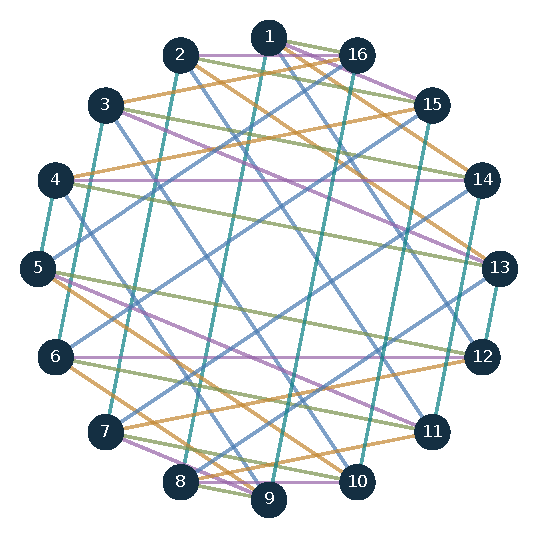
\includegraphics[width=.8\linewidth]{figures/clebsch.pdf}
\caption{Der bedingte Clebsch-Kopplungsgraph. Farben kennzeichnen die fünf perfekten Matchings. Die Kreispositionen und Knotennummern sind nur Zeichnungskonventionen; sie behaupten keine räumliche Einbettung oder physikalische Entfernung.}
\end{figure}

Der gleichgradige Klammerkanal ist auf dem Viererfaktor antisymmetrisch. Bei der in S11 gewählten Normierung $K^\dagger K=I-S=2P_-$ ergibt eine \emph{zusätzlich angenommene} einheitliche Vermittlerenergie und Amplitude in zweiter Ordnung
\begin{equation}
H_{\mathrm{eff}}=-\frac{t^2}{\Delta}K^\dagger K
=\frac{2t^2}{\Delta}P_++\text{Konstante}.
\end{equation}
Der Faktor zwei gegenüber dem vorigen $W$-Modell liegt in der Normierung: $K=\sqrt2W$, entsprechend $g=\sqrt2t$.

\section{Welche Auswahl hier noch hinzukommt}
Die Graphkombinatorik folgt aus der angegebenen Ortslesart. Um daraus einen Vielteilchen-Hamiltonoperator zu erhalten, braucht man außerdem eine Fock- oder Tensorproduktstruktur, Besetzungsbedingungen, die Bedeutung der virtuellen Zustände und ihre Energien. Betragsgleiche Chevalley-Strukturkonstanten wählen noch keine physikalischen Kopplungsstärken in normierten Mehrteilchenzuständen aus. Gleiche $t$ und $\Delta$ müssen dynamisch oder durch eine entsprechend starke Symmetrie des \emph{gesamten} Modells begründet sein.

Auch das Wort „hard-core“ folgt nicht allein aus einer fehlenden Wurzelsumme. Für zwei verschiedene lokale $A_3$-Gewichte am selben Spinorgewicht beträgt das Normquadrat der gesamten Summe sechs; bei gleichem Gewicht acht. Die fünf in S11 sind der $D_5$-Anteil allein. In beiden Fällen ist die Summe zwar keine Wurzel der Norm zwei. Daraus folgt zunächst nur das Fehlen dieses direkten Klammerkanals, keine automatisch verbotene Doppelbesetzung eines noch zu definierenden Fockraums.

Da ein Vektorlabel vier Kanten trägt, muss die effektive Rechnung zudem erklären, wie virtuelle Zustände verschiedenen Bindungen zugeordnet werden. Identische reine Vermittlerlabels können in einem bloßen Zwei-Teilchen-Modell Kreuzterme erzeugen. In einem fest besetzten Vielteilchenraum können verschiedene Loch- und Zuschauerzustände sie dagegen unterscheiden. Genau diese noch offene Belegungsstruktur entscheidet, ob nur der behauptete Paarterm bleibt.

Der Clebsch-Graph enthält keinen vollständigen $K_4$. Daraus folgt nicht, dass der Zustand $\Omega$ unmöglich wäre: Ein verbundener Viererpfad reicht für denselben Kern. Es folgt aber, dass der vollständige Tetramer-Hamiltonoperator nicht einfach die induzierte native Viererstruktur dieses Graphen ist. Ebenso macht uniforme Clebsch-Kopplung daraus keine uniforme Kette. Der Schluss „also $\lambda=J$ in der Kette und damit WZW“ wechselt den Graphen und benötigt einen eigenen Nachweis.

\section{Die berichteten Clusterzahlen}
\par\noindent\begin{tabularx}{\linewidth}{L{74mm}Y}
\toprule
\textbf{Clebsch-Cluster bei $J=1$, nach S11}&\textbf{Berichteter Wert}\\\midrule
Grundenergie&$11{,}045398$\\
Grundzustand&Eindeutiges $\mathrm{SU}(4)$-Singulett, Form $(4,4,4,4)$\\
Erster angeregter Singulettwert&$11{,}561762$; mindestens vier orthogonale Moden, Gap etwa $0{,}516$\\
Erste adjungierte Anregung&$12{,}133537$, Gap etwa $1{,}088$\\
Weitere Multiplets&$20'$ bei $12{,}3228$; $45$ bei $12{,}8751$ und $12{,}9816$\\
Symmetrisches Gewicht pro Kante&$0{,}27613$\\
Symmetrisches Gewicht pro Nichtkante&$0{,}61193$\\
Summe über alle 120 Paare&$60$\\
Produkt aus vier disjunkten $\Omega$-Viererzyklen&$15J$, im Text zugleich als untere Schranke aller solchen Produktformen angegeben\\\bottomrule
\end{tabularx}\par
Die vollständige Clusterdiagonalisierung wurde hier nicht wiederholt. Es handelt sich um numerische Eigenwerte aus S11, nicht um exakte algebraische Eigenzahlen. Die Graphidentitäten sind unabhängig exakt bestätigt; das ist eine andere Evidenzklasse. Ein Rang oder eine Darstellung kann exakt feststehen, während ihre Eigenwerte numerisch berechnet werden.

\begin{grenze}{Neue Singulettprüfung v1.3}
Zwei zusätzliche Läufe im vollen 24024-dimensionalen Singulett-Multiplizitätsraum finden mindestens vier orthogonale Moden bei $11{,}561762122803J$, mit Residuen unter $10^{-8}$. Das alte Dublett ist korrigiert. Eine exakte obere Multiplizitätsschranke und ein neuer Lauf aller Nichtsingulettsektoren fehlen. Die übrigen Tabellenwerte bleiben S11 zugeschrieben.
\end{grenze}
\section{Neue Korrektur: Singulett heißt nicht eindeutig}
S11 behauptet für den \emph{vollständigen} Graphen mit $N=4m$ einen eindeutigen Grundzustand bei $E_0=5m(m-1)J$ und Gap $2J$. Energie und Gap stimmen; die Eindeutigkeit stimmt ab acht Trägern nicht.

Der Hamiltonoperator ist dort die zentrale Transpositionssumme. Auf der Youngform $\lambda=(m,m,m,m)$ wirkt $\mathrm{SU}(4)$ trivial, aber diese Darstellung tritt mit der Specht-Multiplizität $f^\lambda$ auf. Der Grundraum hat deshalb
\begin{equation}
\dim\mathcal H_0=f^{(m,m,m,m)}
=\frac{(4m)!}{\prod_{(r,c)\in(m^4)}h_{rc}}.
\end{equation}
\begin{center}
\begin{tabular}{rrrr}
\toprule $N$&$E_0/J$&Gap$/J$&Grundraumdimension\\\midrule
4&0&2&1\\8&10&2&14\\12&30&2&462\\16&60&2&24024\\\bottomrule
\end{tabular}
\end{center}
Diese Werte wurden hier durch Enumeration aller Youngformen mit höchstens vier Zeilen und exakte Hookformeln geprüft; die gesamten Schur-Weyl-Dimensionen ergeben jeweils $4^N$. Das ist eine konkrete Korrektur des vollständigen Graphen. Sie widerlegt nicht die separat berichtete numerische Eindeutigkeit des Clebsch-Grundzustands, dessen Hamiltonoperator nicht dieselbe zentrale Summe ist.

\section{Neue Präzisierung: Aufzeichnung ist nicht durch die 248 verboten}
\textbf{Operatoren unterscheiden (v1.3):} Das folgende $Q=I-2D$ beschreibt eine gleichkontextige Vierer-Aufzeichnung. Das neue binäre Austauschregister $R=P_+\otimes I+P_-\otimes X$ ist ein anderer Operator und nachweislich nicht Clifford. Seine zusätzliche Ressourcenanforderung widerspricht der folgenden Darstellbarkeit von $Q$ nicht.

Die Sektortrennung aus S11 ist für die \emph{gleichkontextige} Kopplung anschaulich: $Q$ reflektiert den von $\ket{jj}$ aufgespannten Vierraum, der in $\mathrm{Sym}^2(4)$ liegt. Auf $\Lambda^2(4)$ wirkt es als Identität. Entsprechend lässt dieser spezielle Operator den Paaranteil einer idealen $\Omega$-Zelle unverändert. Bei einer anderen Registerbasis gilt die Aussage nicht automatisch; S11 berichtet dafür $1/15$ statt $15/15$ Kontexte.

Der daraus gezogene Schluss „eine Cross-Register-Aufzeichnung ist innerhalb der 248 unmöglich“ geht jedoch über den bewiesenen Satz hinaus. Ein Tensorprodukt von Trägern und zusammengesetzte Operatoren sind nicht auf die irreduziblen \emph{Generatorbestandteile} der Adjungierten beschränkt.

Ein expliziter Gegenbeleg im vorhandenen Vierer-Matrixbaukasten verwendet
\begin{equation}
D=\sum_{j=0}^3\ket{jj}\bra{jj}
=\frac14\left(I\otimes I+Z_1\otimes Z_1+Z_2\otimes Z_2
+Z_1Z_2\otimes Z_1Z_2\right),
\end{equation}
wobei $Z_1,Z_2$ die beiden Pauli-$Z$ im Viererträger sind. Dann gilt
\begin{equation}
Q=I-2D=e^{-i\pi D},\qquad Q^2=I.
\end{equation}
Diese Operatoridentitäten und die Wirkung auf den antisymmetrischen Sektor wurden hier exakt geprüft. Die lokale Matrixalgebra samt zugelassener trägerübergreifender Produkte kann die Kopplung also ausdrücken.

\begin{grenze}{Was dadurch gelöst ist und was offen bleibt}
Gelöst ist die algebraische Darstellbarkeit nach Zulassung einer konkreten Tensorproduktkopplung. Nicht gelöst ist ihre physikalische Verfügbarkeit aus der primitiven TFPT-Quelle. Ein größerer $E_8$-Modul wie die in S11 vorgeschlagene 3875 kann ein möglicher Forschungsweg sein; seine Notwendigkeit folgt nicht aus dem Sektorargument. Die dort genannte Verzweigung und ein tatsächlich geeigneter Aufzeichnungsoperator in diesem Modul sind hier nicht geprüft.
\end{grenze}

\chapter{Zwei Zellen: aus Verbindung wird Dynamik}
\label{ch:two}
\begin{bild}{Aktualisierung v1.5: der Übergang zu vielen Zellen ist genauer}
Kapitel~\ref{ch:scaling15} beweist für ganze wachsende Familien, wann die Lücke bestehen bleibt und wann eine ausdrücklich gewählte innere Transferdynamik kritisch wird. Der exakt bekannte 544D-Stern und die größere C16-Zelle werden dabei nicht verwechselt. Lokale statische Stabilität ist noch keine vollständige dynamische Grenzkontrolle.
\end{bild}
\section{Warum die Zellen beim Verbinden ihre Reinheit verlieren}
Ist eine reduzierte Dichtematrix $\rho_A=\ket\Omega\bra\Omega$ rein, so muss der gemeinsame Zustand bezüglich $A$ und seinem Rest faktorisiert sein. Sein Träger liegt in $\C\Omega\otimes\mathcal H_B$. Sind alle disjunkten Zellmarginalien unverändert rein, ist der Gesamtzustand ein Produkt über die Zellen.

Deshalb können gekoppelte Zellen nicht zugleich unverändert reine $\Omega$-Zustände bleiben und miteinander verschränkt sein. Sie können im Produkt beginnen und dann korrelieren. Oder $\Omega$ bezeichnet eine lokale Verknüpfungsamplitude und nicht die physische Dichtematrix jeder Region. Diese Unterscheidung eröffnet einen konsistenten Weg zu größeren Netzen. \src{S03, §2 und §7}

\section{Ein kleiner exakter Raum in einem großen Hilbertraum}
Zwei vollständige Tetramerzellen mit genau einer Brücke haben
\begin{equation}
H=H_A+H_B+\lambda V,\qquad V=(I+S_{ab})/2,\quad J>0,\ \lambda\ge0.
\end{equation}
Der volle Raum besitzt $4^8=65536$ Dimensionen. Trotzdem bleibt die Entwicklung des Produktzustands in einem zweidimensionalen invarianten Unterraum:
\begin{equation}
\ket0=\ket\Omega_A\ket\Omega_B,\qquad
\ket1=\frac{4S_{ab}-I}{\sqrt{15}}\ket0.
\end{equation}
Die beiden Vektoren sind orthonormal; $H_0\ket0=0$ und $H_0\ket1=4J\ket1$. Es folgt
\begin{equation}
\boxed{H_{\mathrm{red}}=
\begin{pmatrix}
5\lambda/8&\sqrt{15}\lambda/8\\
\sqrt{15}\lambda/8&4J+3\lambda/8
\end{pmatrix}.}
\label{eq:Hred}
\end{equation}
Die Brücke koppelt den Produktgrundzustand an eine gemeinsame adjungierte Anregung. Beide Zellhälften verwenden dabei einen bestimmten 15-dimensionalen Unterraum ihrer jeweils 45-dimensionalen ersten Anregungsfläche. \src{S01, §4; S03, §3; hier auf allen 65536 Komponenten exakt geprüft}

\section{Energie und ein wirklicher Grundzustandsnachweis}
Mit
\begin{equation}
R=\sqrt{16J^2-2J\lambda+\lambda^2}
\end{equation}
lauten die beiden Eigenwerte
\begin{equation}
E_\pm=\frac{4J+\lambda\pm R}{2},\qquad
E_-=\frac{5\lambda}{8}-\frac{15\lambda^2}{256J}
-\frac{15\lambda^3}{4096J^2}+O(\lambda^4/J^3).
\end{equation}
Die negative Korrektur beschreibt die Absenkung gegenüber dem einfachen Produktwert $5\lambda/8$.

Ein exakter Eigenzweig ist noch kein globaler Grundzustandsbeweis. Hier gibt es aber eine zusätzliche Schranke: Der zweite Eigenwert von $H_A+H_B$ ist $2J$. Wegen $\lambda V\ge0$ kann der zweite Eigenwert des gekoppelten $H$ nicht darunter fallen. Solange $E_-<2J$, ist der gefundene Eigenwert also der eindeutige globale Grundwert. Das ist genau der Bereich
\begin{equation}
0\le\lambda<8J,\qquad
\Delta_{\mathrm{gap}}\ge2J-E_-=\frac{R-\lambda}{2}>0.
\label{eq:gapbound}
\end{equation}
Bei $\lambda\ge8J$ endet nur dieser historische Nachweis. Version 1.3 kontrolliert die Konkurrenzsektoren für dasselbe Zweizellenmodell nun bei allen endlichen $\lambda\ge0$. Mit $Q=\sqrt{4J^2+\lambda^2}$ gilt
\begin{equation}
E_0=E_-,\quad E_1=3J+\lambda/2-Q/2,\quad
\Delta_{\mathrm{gap}}=J+(R-Q)/2>J/2.
\label{eq:alllambda13}
\end{equation}
Der Grundzustand bleibt eindeutig; $8J$ und $16J/5$ waren Beweisgrenzen, keine Phasenübergänge. Der vollständige Beweis steht in Kapitel~\ref{ch:audit13}. Er gilt für zwei vollständige Tetramer mit einer Brücke, nicht für beliebig große Netze.

\begin{figure}[H]\centering
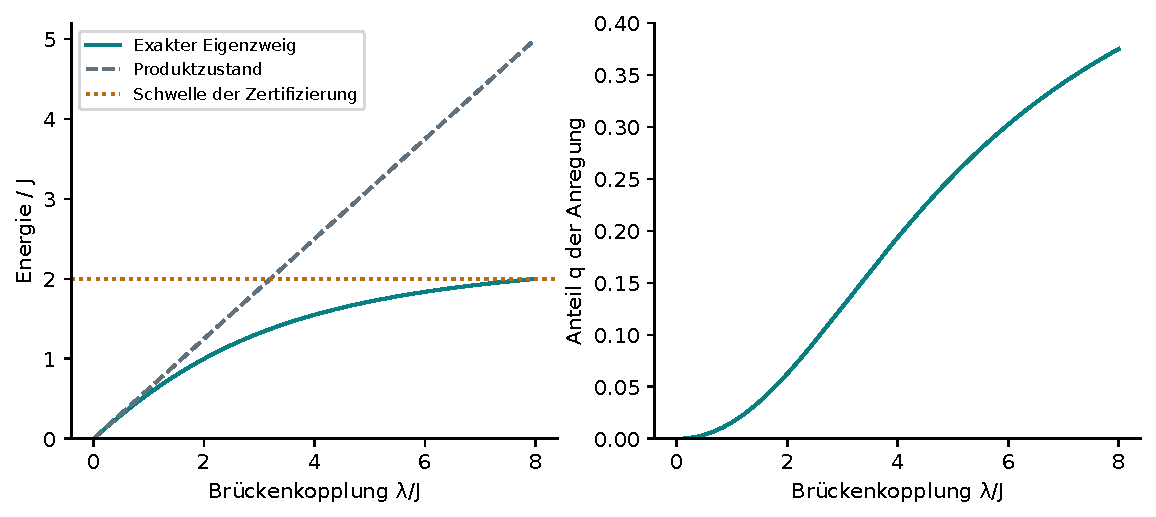
\includegraphics[width=\linewidth]{figures/two_cells.pdf}
\caption{Links der exakte Zweizellen-Eigenzweig und der Produktwert. Die Linie $2J$ illustriert die ältere hinreichende Schranke, nicht die Grenze des neuen allkoppligen Satzes. Rechts der Anregungsanteil $q$. Die Kurven sind berechnete Modellwerte.}
\end{figure}

\begin{center}
\begin{tabular}{rrrr}
\toprule $\lambda/J$&$E_-/J$&Untere Gapgrenze$/J$&Gap nach S08\\\midrule
0&0&2&2\\
0,5&0,29743758&1,70256242&1,922\\
1&0,56350833&1,43649167&1,818\\
2&1&1&1,586\\
3,2&1,37289425&0,62710575&1,340\\
6&1,83772234&0,16227766&1,000\\\bottomrule
\end{tabular}
\end{center}
Die Untergrenze ist nicht der exakte Gap. Die Werte der letzten Spalte sind Quellnumerik. Der ältere Nachweis $\Delta\ge2J-5\lambda/8$ war korrekt, aber schwächer und nur bis $\lambda<16J/5$ positiv.

\section{Verschränkung aus derselben Kopplung}
Der niedrige Eigenzustand lässt sich schreiben als
\begin{equation}
\ket{\Psi_-}=\sqrt{1-q}\ket0-\sqrt q\ket1,
\qquad q=\frac12\left(1-\frac{4J-\lambda/4}{R}\right).
\end{equation}
Seine Zellreduktion besitzt das Spektrum
\begin{equation}
\spec\rho_A=\{1-q,(q/15)^{[15]},0^{[240]}\}.
\end{equation}
Die Entropie in natürlichen Logarithmen ist
\begin{equation}
S_A=-(1-q)\log(1-q)-q\log(q/15).
\end{equation}
Bei $\lambda=J$ sind $q\approx0{,}0158771$ und $S_A\approx0{,}1245231$; bei $\lambda=2J$ gilt $q=1/16$. Schon eine endliche einzelne Brücke macht die lokale Zelle gemischt. Energieabsenkung und Verschränkung sind hier keine unabhängig eingesetzten Zusätze.

Die isolierten Reduktionen von $\Omega$ sind hingegen
\begin{equation}
\rho_k=\frac{P_{\Lambda^k\C^4}}{\binom4k},\qquad k=1,2,3.
\end{equation}
Auf ihrem Träger ist $-\log\rho_k$ skalar. Ihr endlicher modularer Fluss ist dort trivial. Im gekoppelten Zustand entsteht eine modulare Wertdifferenz $\log[15(1-q)/q]$. Sie ist dimensionslos und noch keine physikalische Zeit. Nullräume dürfen dabei nicht mit einem undefinierten Logarithmus behandelt werden. \src{S03, §4 und §6}

\section{Ein Uhrsignal ohne zusätzlich gewählten lokalen Tick}
Starte im Produkt $\ket0$ und lasse denselben konstanten gekoppelten Hamiltonoperator wirken. Dann gilt
\begin{equation}
p_1(t)=\frac{15\lambda^2}{16R^2}\sin^2\left(\frac{Rt}{2\hbar}\right),
\qquad \langle H_A+H_B\rangle_t=4Jp_1(t).
\label{eq:two-clock}
\end{equation}
Bei $\lambda=J$ vereinfacht sich dies zu $p_1(t)=\frac1{16}\sin^2(\sqrt{15}Jt/(2\hbar))$. Der Energieinhalt beider Zellen pulsiert in einem messbaren Muster.

\begin{figure}[H]\centering
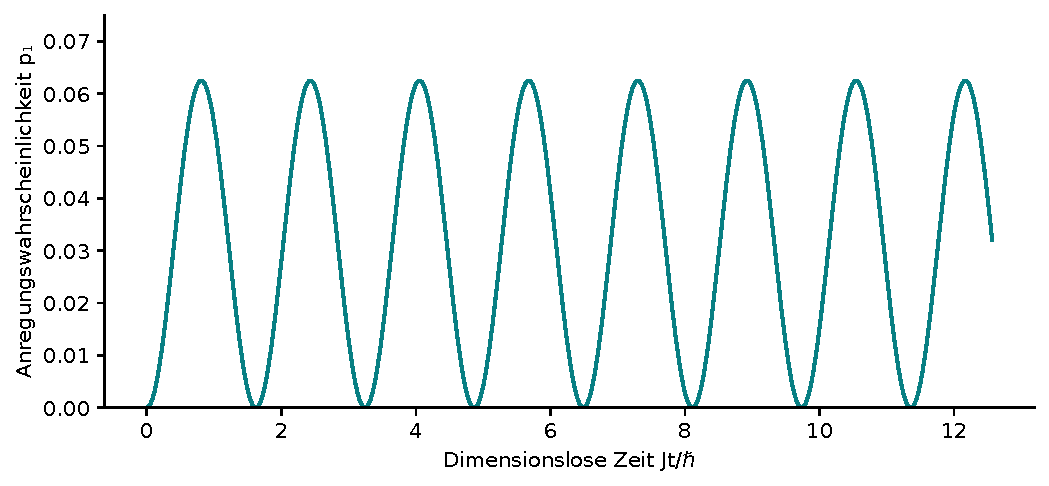
\includegraphics[width=.9\linewidth]{figures/two_cell_clock.pdf}
\caption{Das Zweizellensignal bei $\lambda=J$ und Produktanfangszustand. Seine kleine Amplitude ist Teil der Vorhersage. Der stationäre Grundzustand würde dieses Signal nicht zeigen.}
\end{figure}

Das ist autonome Bewegung unter einem gegebenen $H$, jedoch keine Ableitung einer äußeren Zeit oder von Sekunden. Es ist auch keine Vieranzeigenuhr und nicht der Familienzyklus mit Periode drei. Wiederholte Messungen und ihre gespeicherten Ergebnisse verlangen einen zusätzlichen, ausdrücklich einbezogenen Registerprozess.

\section{Warum viele Zellen noch ein eigener Schritt sind}
\begin{grenze}{Integrierte Trennung v1.6: drei unterschiedliche Transportmodelle}
Die folgenden Zellformeln gehören zu den jeweils benannten Modellen. Neuere Rechnungen zeigen Transport in einer gesetzten Dreiplatz-Wedge-Anordnung und in einer Kompression zweier mikroskopischer Sterne. Das ist nicht automatisch Transport im nativen Modell mit 64 Fermion- und 60 Vermittlermoden pro Bank. Dort erhält reines Vermittlerhopping die Fermionparität jeder Bank. Ein einzelnes Fermion kann dadurch die Bank nicht wechseln. Kapitel~\ref{ch:v16-labor} nennt die positiven endlichen Transportbefunde; Kapitel~\ref{ch:v16-state} benennt die Paritätsschranke und den notwendigen Test einer tatsächlich ungeraden Transportoperation.
\end{grenze}


Ein einzelner eindeutiger Singulettgrundraum besitzt keine logische Zustandsvielfalt. Das Produkt solcher Grundräume bleibt eindimensional. Wer alles auf diese Grundräume projiziert, erhält nur eine skalare Energie. Nichttriviale effektive Dynamik muss Anregungen, Randzustände, Multiplizitäten oder zusätzliche Vakuumsektoren behalten.

Für $N$ vollständige Zellen mit $N-1$ positiven Brücken liefert der Produktzustand
\begin{equation}
E_0\le(N-1)\frac{5\lambda}{8},\quad
\Delta\ge2J-(N-1)\frac{5\lambda}{8}.
\end{equation}
Die einfache Eindeutigkeitsgarantie $\lambda<16J/[5(N-1)]$ verschlechtert sich mit der Zellzahl. Sie beweist keinen thermodynamischen Gap. Zudem kann ein zusammenhängendes Netz von mehr als vier Trägern nicht sämtliche Paarbedingungen mit Nullenergie erfüllen. Diese Frustration ist ein struktureller Befund und muss in jedem skalierenden Modell berücksichtigt werden.

\chapter{Zeit: Takt, Uhrwerk und lesbare Veränderung}
\label{ch:zeit}
\section{Drei Bedeutungen des Wortes Clock}
Eine zyklische Matrix ist zunächst ein Taktmuster. Eine Dynamik sagt, wann welcher Zustand entsteht. Eine Uhr braucht zusätzlich eine beobachtbare Anzeige und eine Kalibrierung. Diese drei Ebenen müssen zusammenpassen.

Die Familienoperation $\sigma$ besitzt Ordnung drei. Ein markierter Lift $c=i\sigma$ erfüllt $c^4=\sigma$ und $c^{12}=I$. Auf Observablen verschwindet die globale Phase $i$ bei der Konjugation; ihre Periode ist dann höchstens drei. Die Ordnung zwölf kann nur relativ zu einer Phasenreferenz sichtbar werden.

Für ein unitäres $A$ gilt am Singulett
\begin{equation}
A^{\otimes4}\Omega=\det(A)\Omega,
\quad\bra\Omega A_1\ket\Omega=\frac{\Tr A}{4},
\quad p_{1j}=\frac{16-|\Tr A|^2}{24}.
\end{equation}
Bei nichtunitären Filtern müssten Normierung und Erfolgswahrscheinlichkeit ergänzt werden. Für den ausgewählten Dreierzyklus ist $|\Tr c|=1$; die Paarenergien sind $5/8$ und die Gesamtenergie $15J/8$ außerhalb der Rückkehrschritte. Die Paartests sehen Periode drei, der phasentreue Überlapp des Lifts Periode zwölf. \src{S08, §4; S01, §5}

\section{Warum die Paarenergien unter dem Tetramer stillstehen}
Der vollständige gleichgewichtete Tetramer-Hamiltonoperator ist eine zentrale Transpositionssumme. Deshalb kommutiert er mit jedem $S_{ij}$ und jedem $P^+_{ij}$. Die Paarenergien ändern sich unter seiner freien Entwicklung nicht. Eine Tabelle, die nacheinander einen lokalen $c$-Tick anwendet, ist somit kein Beweis, dass genau diese Anzeige unter $H_{\mathrm{tet}}$ von selbst läuft.

Auch der bedingte Dreiträgersektor $\Lambda^3\C^4\cong\overline4$ bildet eine einzige irreduzible $\mathrm{SU}(4)$-Darstellung. Ein vollständig $\mathrm{SU}(4)$-invarianter Systemgenerator wirkt dort nach Schurs Lemma skalar. Zusätzliche invariant gebaute Terme spalten die vier bedingten Lesarten nicht einfach auf. Das ist die stärkere Form des in S07 zunächst über drei Energieniveaus beschriebenen Hindernisses.

\section{Eine laufende lokale Anzeige im gesetzten Modell}
Ein präparierter nichtstationärer Zustand kann dennoch unter demselben Tetramer laufen. Für einen lokalen spurfreien hermiteschen Pauli $A$ mit $A^2=I$ setze
\begin{equation}
\ket{\psi(0)}=e^{-i\pi A_1/4}\Omega
=\frac{\Omega-iA_1\Omega}{\sqrt2}.
\end{equation}
Da $H_{\mathrm{tet}}A_1\Omega=2JA_1\Omega$, folgt
\begin{equation}
\langle A_1\rangle_t=-\sin(2Jt/\hbar),\qquad
\langle A_j\rangle_t=\tfrac13\sin(2Jt/\hbar)\quad(j\ne1).
\end{equation}
Die lokalen Anzeigen oszillieren gegeneinander; ihre Summe bleibt null. Die Periode ist $\pi\hbar/J$. Präparation, Ausleserichtung und die Kalibrierung von $J$ sind weitere Eingaben. \src{S01, §5.2}

\begin{figure}[H]\centering
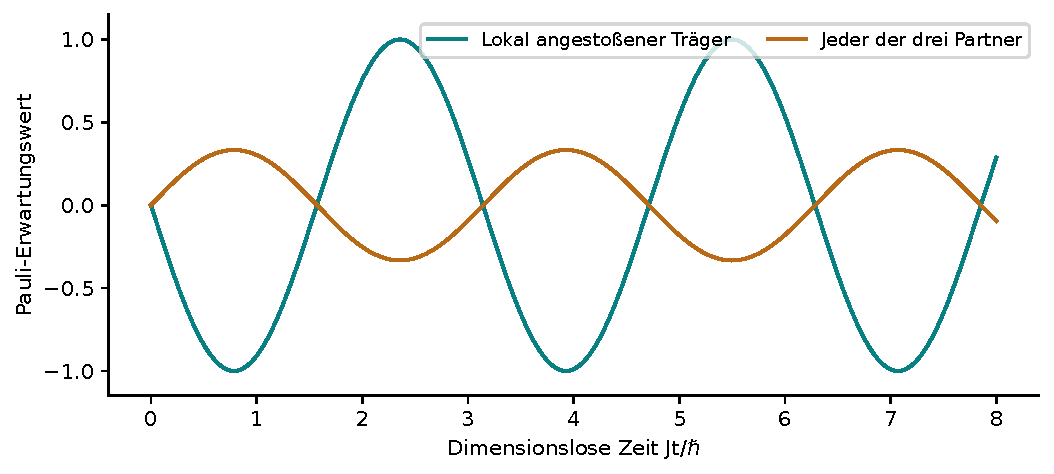
\includegraphics[width=.94\linewidth]{figures/clock.pdf}
\caption{Ein lesbares Uhrsignal trotz konstanter Paarenergien. Unterschiedliche Observablen beantworten unterschiedliche Fragen.}
\end{figure}

\section{Eine relationale Viereruhr ist konstruierbar}
Zerlege $\Omega=\frac12\sum_{a=0}^3\ket a_C\ket{\omega_a}_S$. Die vier $\omega_a$ sind orthonormal. Wähle zusätzlich
\begin{equation}
h=\frac{\hbar\omega}{2}\operatorname{diag}(-3,-1,1,3),\quad
H_C=h_0,\quad H_S=h_1+h_2+h_3.
\end{equation}
Weil jedes Wort von $\Omega$ jedes Energielabel einmal enthält, gilt $(H_C+H_S)\Omega=0$. Für
\begin{equation}
\ket t_C=\frac12\sum_a e^{-i\epsilon_at/\hbar}\ket a,
\qquad \ket{\psi(t)}_S=2\,{}_C\bra t\Omega\rangle
\end{equation}
erhält man $\psi(t)=e^{-iH_St/\hbar}\psi(0)$. Die Zeiten $t_k=k\pi/(2\omega)$ liefern vier orthogonale Anzeigen. Global ist der Zustand stationär, bedingt auf die Uhranzeige entwickelt sich das System. Das ist eine konkrete Page-Wootters-Konstruktion, aber mit zusätzlich gewählter Basis, Energieleiter und Fourierauslesung. \src{S01, §5.4; S05, §8; S06}

Eine rein diskrete Alternative aus S05 verwendet den Viererzyklus $R\ket j=\ket{j+1\bmod4}$. In der Zweiqubitkodierung lässt er sich aus CNOT und Pauli-$X$ bauen. Mit $U_C=R$ und $U_S=-R^{\otimes3}$ gilt
\begin{equation}
(U_C\otimes U_S)\Omega=\Omega,\qquad U_S\omega_a=\omega_{a+1}.
\end{equation}
Dieser Tick ist nicht der ausgezeichnete Familienzyklus. Die Existenz einer Uhr ist damit konkret; ihre eindeutige Quellauswahl bleibt offen. Eine experimentelle Illustration des allgemeinen relationalen Zeitgedankens findet sich bei \href{https://arxiv.org/abs/1310.4691}{Moreva et al. [E3]}.

\section{Warum ein Logarithmus noch keine Sekunde ist}
Aus $\lambda^n=e^{-n\delta}$ folgt $\delta=-\log\lambda$. Die historischen Größen $6\log(3/2)$ und $6\log3$ beschreiben deshalb sechsfach wiederholte Faktoren $(2/3)^6$ und $(1/3)^6$. Eine physikalische Rate ist erst $\delta/\tau$ für einen festgelegten Schritt $\tau$.

Eine dimensionslose Theorie muss keinen menschlichen Meter oder eine Sekunde absolut auswählen. Sie muss jedoch die beobachtbaren Verhältnisse und eine konsistente Relation ihrer Skalen bestimmen. Der Vermittlungsansatz lokalisiert die Energieskala auf $t^2/\Delta$, leitet aber weder $t$ noch $\Delta$ aus der algebraischen Struktur allein her.

\chapter{Die ausführbare Präparation und der Mehrzeittest}
\label{ch:echo}
\begin{bild}{Verschiedene Präparationsverträge bleiben getrennt}
Dieses Kapitel bewahrt die ursprüngliche endliche Schaltung mit Erfolg $3/32$ aus dem vorausgesetzten Zweisingulett-Eingang. Der neue Stern-Spektralfilter erreicht $1/6$ aus demselben Eingang, setzt aber kontrollierte kontinuierliche Pulse voraus. Kapitel~\ref{ch:execution13} beginnt dagegen bei $\ket{0123}$, benutzt wiederholt dasselbe Austauschregister und nähert sich $\Omega$ mit vollständig berechneten Fehlzweigen. Bei endlicher Rundenzahl ist diese dritte Variante nicht exakt. Ihre Ressourcen und Erfolgszahlen dürfen nicht vermischt werden.
\end{bild}
\section{Was S02 tatsächlich geschlossen hat}
Die Präparationsnotiz S02 geht über den abstrakten Satz „$\Omega$ existiert“ hinaus. Sie beschreibt eine konkrete Schaltung, die aus einem einfachen Eingang den Zustand mit Erfolgsanzeige herstellt, anschließend ein Register schreibt und die Rückkehr ausliest. Laut Quelle wurde die Schaltung exakt simuliert, nicht auf Hardware ausgeführt. Ihr Zugriff auf zusätzliche Hilfssysteme und Nicht-Clifford-Operationen ist ausdrücklich angenommen.

Die gemeinsame Wechselwirkung ist der kohärent kontrollierte Swap
\begin{equation}
F_{R;ij}=\ket0\bra0_R\otimes I+\ket1\bra1_R\otimes S_{ij}.
\end{equation}
Ein passender Generator ist
\begin{equation}
H_{\mathrm{int}}=\hbar g\ket1\bra1_R\otimes P^-_{ij},\quad
g\tau=\pi\quad\Longrightarrow\quad e^{-iH_{\mathrm{int}}\tau/\hbar}=F_{R;ij}.
\end{equation}
Der Beweis nutzt nur die Projektoreigenschaft $G^2=G$: $e^{-i\pi G}=I-2G$.

Die Swap-Identität $S=\frac14\sum_{v=0}^{15}P_v\otimes P_v$ zeigt, wie der Generator im Quell-Pauli-Raum liegt:
\begin{equation}
G=\frac3{16}(I-Z_R)\otimes I
-\frac1{16}\sum_{v=1}^{15}I_R\otimes P_v\otimes P_v
+\frac1{16}\sum_{v=1}^{15}Z_R\otimes P_v\otimes P_v.
\end{equation}
Die Terme kommutieren. Die algebraische Schreibbarkeit ist genau; physische Adressierbarkeit, Pulsfläche, Reset und Messbarkeit folgen daraus noch nicht.

\section{Die zusätzliche Ressource bleibt sichtbar}
Der benötigte Zustand $\Omega$ ist in der Acht-Qubit-Kodierung kein Stabilizerzustand. Schon für einen nichttrivialen lokalen Pauli gilt
\begin{equation}
\langle P^{(i)}P^{(j)}\rangle_\Omega=-\frac13,
\end{equation}
während reine Qubit-Stabilizerzustände für Pauli-Observablen nur $0,\pm1$ liefern. Ebenso ist der Paarreduktionsrang sechs keine Zweierpotenz. Eine exakte Präparation aus einem Stabilizer-Eingang benötigt deshalb eine zusätzliche Ressource, etwa einen passenden Nicht-Clifford-Zugriff. Kontinuierlicher Austausch kann die Cliffordklasse verlassen, beseitigt aber allein nicht die genannte Singulett-Erhaltungsgröße.

Eine kontrollierte Qubitvertauschung besitzt die Folge
\begin{equation}
\mathrm{CX}(a,b);\quad \mathrm{CCX}(R,b,a);\quad\mathrm{CX}(a,b).
\end{equation}
Zwei solche Fredkin-Bausteine vertauschen zwei Ququarts. Der Toffoli-Teil ist nicht Clifford. S02 löst ihn in Clifford- und sieben $T/T^\dagger$-Gatter auf, mit $T=\operatorname{diag}(1,e^{i\pi/4})$. Diese Sieben ist eine transparente Kostenobergrenze der dort gewählten Zerlegung, keine behauptete globale Minimalität.

Ein Nicht-Stabilizer-Hilfszustand oder ein entsprechender Nicht-Clifford-Puls kann die fehlende Ressource liefern. Ihre allgemeine Rolle in der Quantenrechnung ist bekannt. Ihre physikalische Herkunft aus TFPT ist eine andere Frage. \href{https://arxiv.org/abs/quant-ph/0403025}{Bravyi und Kitaev [E4]}

\section{Wie der Filter den Zustand erzeugt}
Der einfache Eingang lautet
\begin{equation}
\chi_0=\frac{\ket{01}-\ket{10}}{\sqrt2}
\otimes\frac{\ket{23}-\ket{32}}{\sqrt2}.
\end{equation}
Er ist mit dem in S02 angenommenen Clifford-Baukasten präparierbar und besitzt $\Omega$-Anteil $1/6$. Der Antisymmetrisierer ist
\begin{equation}
A_4=\ket\Omega\bra\Omega
=\frac1{24}\sum_{\pi\in S_4}\operatorname{sgn}(\pi)U_\pi.
\end{equation}
Die konkrete Schaltung erzeugt 32 Kontrollzweige, von denen 24 die Permutationen tragen. Acht ungültige Zweige werden markiert. Nach Interferenz und Erfolgsselektion ist der implementierte Operator
\begin{equation}
K_{\mathrm{prep}}=\frac1{32}\sum_{\pi\in S_4}\operatorname{sgn}(\pi)U_\pi
=\frac34A_4.
\end{equation}
Somit gilt
\begin{equation}
p_{\mathrm{prep}}=\frac9{16}\frac16=\frac3{32}=9{,}375\%.
\end{equation}
Der erfolgreiche Zweig ist exakt $\Omega$. Die restlichen $29/32$ Versuche sind Misserfolge und dürfen nicht unsichtbar werden. Bei unabhängigen Neuansätzen benötigt man im Mittel $32/3$ Versuche. Das ist eine heraldierte Präparation, kein deterministischer Kühlmechanismus.

\section{Das ursprüngliche Echo: eins gegen siebzehn Zweiunddreißigstel}
Für $S=S_{01}$ schreibe $V=H_RF_{R;01}H_R$. Dann
\begin{equation}
V(\ket0_R\otimes\psi)=\ket0_R\otimes P_+\psi+\ket1_R\otimes P_-\psi,
\quad V^2=I.
\end{equation}
Ein ignorierter frischer Pointer erzeugt
\begin{equation}
\Delta_S(\rho)=\tfrac12(\rho+S\rho S),\qquad\Delta_S^2=\Delta_S.
\end{equation}
Diese \emph{binäre Swap-Aufzeichnung} ist ein anderer Kanal als die 15-Kontext-Mischung mit Faktor $3/7$.

Vor der Aufzeichnung wird auf einem Träger ein lokaler Dreierzyklus $c$ mit $c^3=I$ und $\Tr c=1$ angewendet. Ohne diesen Tick wäre $\Omega$ bereits Swap-Eigenzustand und beide Ausführungen wären für den Test gleich. Danach folgen zwei Anwendungen von $V$, Rücknahme von $c$ und der gleiche Endfilter wie bei der Präparation. Es gilt
\begin{equation}
\langle c_0\Omega|S_{01}|c_0\Omega\rangle=\frac14,
\quad p_+=\frac58,\quad p_-=\frac38.
\end{equation}
Mit demselben kohärenten Pointer hebt die zweite Anwendung die erste auf. Mit frischen Pointern bleibt die Dephasierung. Der normierte Rückkehrwert ist daher
\begin{equation}
F_{\mathrm{behalten}}=1,\qquad
F_{\mathrm{frisch}}=p_+^2+p_-^2=\frac{17}{32}.
\label{eq:originalecho}
\end{equation}

\begin{figure}[H]\centering
\begin{tikzpicture}[node distance=8mm]
\node[box,text width=25mm] (p) at (0,0) {$\Omega$ erfolgreich\\präpariert};
\node[box,text width=19mm] (c) at (3,0) {Lokaler\\Tick};
\node[box,text width=35mm] (r) at (6.8,.9) {$V$, dann $V$\\gleicher Pointer};
\node[openbox,text width=35mm] (f) at (6.8,-1) {$V$, dann $V$\\frische Pointer};
\node[box,text width=24mm] (e) at (10.8,0) {Tick zurück\\Endfilter};
\draw[arr] (p)--(c);\draw[arr] (c)--(r);\draw[arr] (c)--(f);
\draw[arr] (r)--(e);\draw[arr] (f)--(e);
\end{tikzpicture}
\caption{Die Zweige stimmen nach der ersten reduzierten Aufzeichnung überein. Erst die Fortsetzung unterscheidet, ob die erste Aufzeichnung kohärent verfügbar bleibt.}
\end{figure}

\section{Die wirklichen Erfolgswahrscheinlichkeiten}
\begin{bild}{Integriertes Update v1.6: Rohdaten statt nur Rückkehrquotient}
Das neue Ein-Record-Präparationsprotokoll und seine rückwärts ausgeführte Schlussprüfung liefern für die vollständige Vier-Record-Folge die Rohwahrscheinlichkeiten $9/64$ bei kohärent behaltenem Register und $153/2048$ bei frischen Registern. Ihr Verhältnis ist weiterhin $17/32$. Das erste Ergebnis enthält beide Faktoren $3/8$ für Präparation und Schlussprüfung. Die folgenden älteren Ausbeuten bleiben für ihre jeweiligen Filterprotokolle gültig, sind aber nicht mehr die günstigste hier dokumentierte Realisierung. Kapitel~\ref{ch:v16-labor} beschreibt die konkrete neue Folge und ihre Ressourcen.
\end{bild}


Der Endfilter hat den Effekt $K_{\mathrm{prep}}^\dagger K_{\mathrm{prep}}=(9/16)A_4$. Seine beobachtbare Erfolgsrate ist deshalb $(9/16)F$, nicht $F$ selbst.
\par\noindent\begin{tabularx}{\linewidth}{L{68mm}Y Y}
\toprule
\textbf{Statistik}&\textbf{Behalten}&\textbf{Frisch}\\\midrule
$\Omega$-Rückkehr, bedingt auf Präparation&$1$&$17/32$\\
Endfilter erfolgreich, bedingt auf Präparation&$9/16$&$153/512$\\
Beide Filter erfolgreich, je begonnenem Versuch&$27/512$&$459/16384$\\
Alle übrigen Ausgänge&$485/512$&$15925/16384$\\\bottomrule
\end{tabularx}\par
Die gemeinsamen Erfolgsraten sind etwa $5{,}2734\%$ und $2{,}8015\%$. Ein hoher bedingter Rückkehrwert ist also keine hohe Gesamtausbeute.

Nach $n$ Aufzeichnungen mit demselben Pointer alterniert $F$ zwischen eins für gerade $n$ und $17/32$ für ungerade $n$. Bei frischen Pointern bleibt es ab $n=1$ bei $17/32$. Alle einzelnen Träger bleiben dabei maximal gemischt. Die unterscheidende Information sitzt in zugänglichen Korrelationen.

Bei Pointerdephasierung mit verbleibender Kohärenz $0\le\eta\le1$ ergibt das in S02 festgelegte Modell
\begin{equation}
F(\eta)=\frac{17+15\eta}{32}.
\end{equation}
Vollständige Dephasierung zerstört das Echo; ohne Tick liefern beide Zweige eins. Ein reiner Pointer-$Z$-Fehler ergibt $F=1/16$. Die Quelle beschreibt zudem Negativkontrollen ohne Permutationsvorzeichen, ohne Aufzeichnungs-Swaps und mit fälschlich wiederverwendetem Pointer.

\section{Neue Fortsetzung: der maximal ausgeglichene Echovergleich}
\status{Eigene exakte Ergänzung dieser Synthese.} Man kann die gleiche Messfrage für einen beliebigen lokalen unitären Tick $A$ ausrechnen. Setze
\begin{equation}
s=\langle A_0\Omega|S_{01}|A_0\Omega\rangle
=\frac{4-|\Tr A|^2}{12}.
\end{equation}
Die beiden Swap-Gewichte sind $(1\pm s)/2$. Daher
\begin{equation}
F_{\mathrm{frisch}}=\frac{1+s^2}{2},\qquad
F_{\mathrm{behalten}}-F_{\mathrm{frisch}}=\frac{1-s^2}{2}\le\frac12.
\label{eq:optimal}
\end{equation}
Der Kontrast dieser Rückkehrstatistik ist maximal, wenn $s=0$, also $|\Tr A|^2=4$. Ein einzelnes CNOT innerhalb des Viererträgers erfüllt $\Tr A=2$. Es permutiert dieselbe Menge von 60 Stabilizerprojektoren. Damit liefert der vorhandene lokale Tick-Baukasten die klarere Variante
\begin{equation}
\boxed{F_{\mathrm{behalten}}=1,\qquad F_{\mathrm{frisch}}=\frac12.}
\end{equation}
Mit denselben Filterfaktoren sind die gemeinsamen Rohwahrscheinlichkeiten $27/512$ und $27/1024$. Das Dephasierungsmodell vereinfacht sich zu $F(\eta)=(1+\eta)/2$.

Die neue Variante wurde auf dem expliziten ganzzahligen $\Omega$-Tensor und der vollständigen Standardprojektormenge nachgerechnet. Der gesamte ursprüngliche 20-Qubit-Schaltungsexport wurde hier nicht neu kompiliert. Die Aussage ist ein mathematisch konkreter Anschluss und keine nachträgliche Änderung des in S02 eingefrorenen Haupttests. „Maximal“ bezieht sich auf \eqref{eq:optimal}, also genau diese Rückkehrmessung mit einem lokalen Tick und binärer Swap-Dephasierung, nicht auf alle denkbaren Unterscheidungsprotokolle.

\begin{figure}[H]\centering
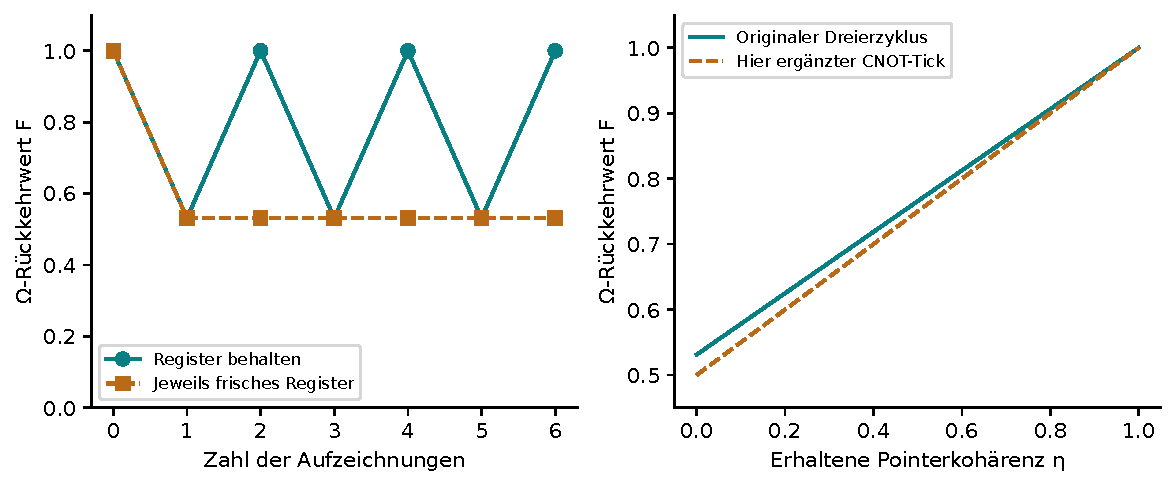
\includegraphics[width=\linewidth]{figures/echo.pdf}
\caption{Links das ursprüngliche Mehrzeitecho. Rechts die ursprüngliche und die neu ergänzte ausgeglichene Variante unter demselben vorgegebenen Pointer-Dephasierungsmodell. Es sind Vorhersagekurven, keine experimentellen Messpunkte.}
\end{figure}

Ein einfaches robustes Zertifikat verbindet die neue Variante mit der Zellprüfung: Falls $\bra\Omega\rho\ket\Omega\ge1-\varepsilon$, weicht jede der idealen Ausgangswahrscheinlichkeiten unter denselben fehlerfreien Folgekanälen um höchstens $\sqrt\varepsilon$ ab. Der Kontrast ist daher mindestens $1/2-2\sqrt\varepsilon$. Das ist eine konservative Schranke aus Spurdistanz und ihrer Kontraktivität, keine vollständige Hardwarefehleranalyse.

\section{Ressourcen und Beweisgrenze der Originalschaltung}
\par\noindent\begin{tabularx}{\linewidth}{Y r}
\toprule \textbf{Ressource nach S02}&\textbf{Anzahl}\\\midrule
Systemqubits&8\\Filterhilfsqubits, wiederverwendet&10\\Pointerplätze&2\\Insgesamt reservierte Qubits&20\\Klassische Erfolgsbits beider Filter&12\\Toffoli-Gatter&574\\Weitere CNOT vor Toffoliauflösung&382\\Hadamard&26\\Pauli-$X$ / Pauli-$Z$&276 / 26\\$T/T^\dagger$ in der gewählten Auflösung&4018\\\bottomrule
\end{tabularx}\par
Ein einzelner Filter verwendet 285 Toffolis. Routing, Fehlerkorrektur, reale Pulse und die Herstellung geeigneter Hilfszustände sind nicht enthalten. Laut S02 bestehen 598 benannte Bedingungen; normale und optimierte Ausführung sowie der unabhängige Paketlauf erzeugten identische Dateien. Die exportierten Hauptschaltungen wurden erneut aus ihren OpenQASM-Zeilen ausgeführt; die vollständigen Clifford+$T$-Varianten waren durch lokale Matrixidentität und Ersetzung zertifiziert, nicht zusätzlich als komplette komplexe 20-Qubit-Vektoren simuliert.

Die Vorhersagedatei wurde laut Quelle am 14. September um 05:51:45 UTC vor dem neuen Prüflauf fixiert. Das ist ein interner Simulationsvertrag mit analytischen Zielwerten, keine externe Studienregistrierung. Das Echo unterscheidet zwei konkrete Ergänzungen derselben ersten Schattenregel. Es identifiziert nicht allein einen einzigartigen Universalraum.

\chapter{Von der Kette zur E\texorpdfstring{$_8$}{8}-Naht}
\label{ch:seam}
\section{Ein wichtiger Modellwechsel}
Das Zweizellenmodell benutzt zwei vollständige Vierergraphen mit einer Brücke. Die Vielzellenrechnung in S08 benutzt dagegen Vierersegmente mit nächster Nachbarschaft. Bei $\lambda=J$ wird erst dieses zweite Modell eine uniforme Kette. Derselbe isolierte Singulettzustand garantiert keine identischen Anregungen und keinen identischen Grenzwert.

\begin{figure}[H]\centering
\begin{tikzpicture}[x=1cm,y=1cm]
\foreach \i in {0,...,7}{\fill[navy] (1.4*\i,0) circle (.10);}
\foreach \i in {0,1,2,4,5,6}{\draw[teal,very thick] (1.4*\i,0)--(1.4*\i+1.4,0);}
\draw[amber,very thick] (4.2,0)--node[above,font=\small]{$\lambda$}(5.6,0);
\node[font=\sffamily\small,text=slate] at (2.1,-.65){Vierersegment mit drei Kanten};
\node[font=\sffamily\small,text=slate] at (7.7,-.65){Vierersegment mit drei Kanten};
\node[font=\sffamily\small,text=navy] at (4.9,1){Uniforme Kette erst bei $\lambda=J$};
\end{tikzpicture}
\caption{Die Kettengeometrie der WZW-Vergleichsrechnung. Sie ist weder der vollständige Tetramergraph noch der Clebsch-Graph.}
\end{figure}

S08 berichtet für offene Ketten die folgenden Lücken in Einheiten $J$:
\begin{center}
\begin{tabular}{rrrr}
\toprule $\lambda/J$&8 Träger&12 Träger&16 Träger\\\midrule
$1/4$&0,2664&0,2552&0,2497\\
$1/2$&0,2299&0,2029&0,1890\\
1&0,1759&0,1273&0,1002\\\bottomrule
\end{tabular}
\end{center}
Bei schwacher Brücke ändern sich die endlichen Werte wenig, bei uniformer Kopplung fallen sie. Das stützt einen Phasenunterschied. Es beweist aus diesen wenigen Größen allein keinen strikt positiven thermodynamischen Gap für jedes $\lambda<J$. S06 weist außerdem darauf hin, dass der ursprüngliche 16-Träger-Prüfer eine ausgewählte Darstellungsfamilie untersucht. Eine daraus erhaltene Anregung ist ohne Ausschluss der übrigen Sektoren kein global zertifizierter erster Gap.

\section{Warum die SU(4)-WZW-Theorie hier plausibel ist}
Für den uniformen periodischen Austauschring liefern die Quellen $\Delta n\approx3{,}700$ bei acht und $3{,}663$ bei zwölf Trägern. Der bekannte Vergleich lautet
\begin{equation}
v=\pi/4,\qquad h(4)=3/8,\qquad c=3,
\qquad 2\pi v(h+\bar h)=\frac{3\pi^2}{8}\approx3{,}70110.
\end{equation}
Die Sutherland-Grundenergie pro Träger ist
\begin{equation}
e_\infty=1-\frac{\pi}{8}-\frac34\log2\approx0{,}087439,
\end{equation}
für $H=\sum(1+P)/2$. S08 nennt die Extrapolation $0{,}08773$ und $c_{\mathrm{fit}}=3{,}16$. Diese endlichen Zahlen passen zur $\mathrm{SU}(4)_1$-WZW-Beschreibung des Kettenmodells. Die allgemeine Verbindung von SU(N)-Spinketten und WZW-Niedrigenergiesektoren wird unabhängig in der Literatur untersucht. \href{https://arxiv.org/abs/0806.2563}{Führinger et al. [E5]}

\begin{bild}{Aus vielen Saitenbewegungen entsteht ein glatter Ton}
Ein Gitter besteht aus einzelnen Stellen. Bei großen Wellenlängen kann seine Bewegung durch ein kontinuierliches Feld beschrieben werden, ähnlich wie eine Saite im Alltag glatt wirkt, obwohl Materie nicht kontinuierlich aufgebaut ist. Das bedeutet nicht, dass jeder andere Graph denselben Ton oder dieselbe Feldtheorie besitzt.
\end{bild}

\section{Die Naht braucht mehr als die Zahl acht}
Die zentrale Ladung ist eine Kennzahl einer konformen Feldtheorie. Für die chiralen Niveau-1-Faktoren gilt
\begin{equation}
c(D_5)=\frac{45}{1+8}=5,\quad
c(A_3)=\frac{15}{1+4}=3,\quad
c(E_8)=\frac{248}{1+30}=8.
\end{equation}
Das Produkt hat also schon vor einer Kopplung $c=5+3=8$. Ein später gefundener Wert acht allein ist kein Beweis einer $E_8$-Erweiterung und kein Beweis eines Kondo-Flusses.

Die konkretere Struktur ist die diagonale $\Z_4$-Verklebung:
\begin{center}
\begin{tabular}{ccccc}
\toprule Klasse&$D_5$-Sektor&$A_3$-Sektor&Gewichte&Neue Ströme\\\midrule
0&Vakuum&Vakuum&$0+0$&$45+15$ bei Stufe 1\\
1&16&4&$5/8+3/8=1$&64\\
2&10&6&$1/2+1/2=1$&60\\
3&$\overline{16}$&$\overline4$&$5/8+3/8=1$&64\\\bottomrule
\end{tabular}
\end{center}
Die Erweiterung ergänzt die 60 ursprünglichen Gewicht-1-Ströme um $64+60+64$, insgesamt 248. Auf der Gitterseite entspricht sie den vier Glue-Klassen. S11 nennt
\begin{equation}
\Theta_{E_8}=1+240q+2160q^2+6720q^3+\cdots,
\quad\frac{\Theta_{E_8}}{\eta^8}=q^{-1/3}(1+248q+4124q^2+\cdots).
\end{equation}
Die abstrakte Gittererweiterung ist konkret. Ihr nativer physischer Aufbau muss zusätzlich Operatorprodukte, Cocycle-Phasen, Adjunktion, Domänen und Energieabschätzungen kontrollieren. Der allgemeine Rahmen konformer Einbettungen und Simple-Current-Erweiterungen ist Literaturhintergrund, keine unabhängige TFPT-Bestätigung. \href{https://arxiv.org/abs/1210.6602}{Kac et al. [E6]}

\section{Warum „Z\texorpdfstring{$_4$}{4}-Eichung“ präzisiert werden muss}
S11 ersetzt die frühere Kondo-Zielbeschreibung sinnvoll durch eine konkrete Erweiterungsaufgabe. Die Kurzschreibweise eines Quotienten durch $\Z_4$ kann jedoch verschiedene Operationen meinen. Nur auf invariante Zustände des ursprünglichen Produkts zu projizieren ist nicht dasselbe wie eine Simple-Current-Erweiterung mit den nötigen zusätzlichen beziehungsweise entsprechend gekoppelten Sektoren.

Ein Gittermodell muss angeben, welche Randbedingungen, Ladungssektoren und lokalen Operatoren enthalten sind. Die 248 Zustände auf Stufe eins sind dann ein notwendiger früher Test. Sie allein beweisen noch nicht die vollständigen Operatorprodukte oder den analytischen Skalierungslimes.

S11 schlägt dafür einen SU(4)-Ring zusammen mit zehn Majorana-Moden vor. Deren $D_5$-Sektoren besitzen die Gewichte $0,1/2,5/8,5/8$. Auf der Ringseite sollen die vier Restklassen der Trägerzahl die $A_3$-Sektoren organisieren. Die berichteten endlichen Werte lauten:
\begin{center}
\begin{tabular}{rrrrr}
\toprule $n$&$n\bmod4$&Sektordimension&$E_0/J$&Extrahiertes $x$\\\midrule
5&1&60&0,690983&0,507\\
6&2&180&0,697224&0,460\\
7&3&630&0,634808&0,282\\
8&0&2520&0,539495&$-0,009$\\
9&1&7560&0,898579&0,454\\
10&2&25200&0,998465&0,501\\
11&3&92400&0,993060&0,320\\
12&0&369600&0,944508&$-0,005$\\
13&1&1201200&1,205482&0,431\\\bottomrule
\end{tabular}
\end{center}
Die Werte wurden aus $E_0=ne_\infty-\pi v(c-12x)/(6n)$ gewonnen. In S11 werden die ungeraden Paare gemittelt und mit $3/8$ verglichen, der Zweiersektor mit $1/2$. Diese Sektorzuordnung hängt an den Randbedingungen und endlichen Korrekturen; eine chirale Gewichtstabelle darf nicht unbesehen mit jeder nichtchiralen Ringskalierungsdimension gleichgesetzt werden. Die Daten sind hier als berichtete Hinweise erhalten, nicht neu reproduziert.

\section{Die Chiralitätslücke}
\begin{grenze}{Integrierte Präzisierung v1.6: dieselbe Algebra ist noch nicht dasselbe Feld}
Der signierte native Kopplungstensor passt nach einer festen Phasenkonvention zu den entsprechenden $E_8$-Wurzelprodukten. Die bekannte Gitter-Vertexalgebra liefert dafür ebenfalls ein Operatorprodukt. Das verknüpft die Strukturkonstanten; es identifiziert nicht automatisch die physische Reaktion $b^\dagger ff$ mit einem chiralen Vertexfeld. Die Gewicht-1-Ströme von $V_{E_8}$ sind bosonisch. Ebenso entfernt eine Faltung der Brillouinzone keine Spiegelmoden: Der explizit geprüfte einfache Weyl-Walk besitzt weiterhin entgegengesetzte Chiralitäten. Die Unterscheidung von innerem Spinor, räumlicher Bewegung und chiraler Feldtheorie wird in Kapitel~\ref{ch:v16-operations} durchgehalten.
\end{grenze}


Eine gewöhnliche kritische SU(4)-Kette hat links- und rechtslaufende Sektoren, mit $c_L=c_R=3$. Die übliche Kennzahl heißt dabei $c=3$, nicht sechs. Die chirale Differenz ist null. Eine rein chirale $E_8$-Naht hat dagegen Differenz acht. Ein zusätzliches ebenfalls nichtchirales $D_5$-Modell ändert daran nichts.

Eine mögliche physikalische Architektur benutzt einen zweidimensionalen Bulk, in dem gegenläufige innere Moden gegappt werden und chirale Randmoden bleiben. Aber ein solcher 2+1D-Bulk ist noch keine 3+1D-Raumzeit. Auch ein holomorpher Rand bedeutet nicht, dass der passende Bulk „leer“ ist: Eine gapped invertierbare Phase kann eine nichttriviale topologische Antwort tragen.

\section{Zwei Vierteldrehungen und der Index}
Die innere Glue-$\Z_4$ wirkt auf den 248 Strömen mit Phasen $1,i,-1,-i$ auf Sektoren der Größen $60,64,60,64$. Ihre Spur ist null. Die geometrische Vierteldrehung $e^{i\pi L_0/2}$ hat auf Stufe eins dagegen Spur $248i$. Die Operatoren sind somit nicht identisch. Eine Clock kann eine geometrische Drehung mit innerem Twist kombinieren; die beiden Faktoren bleiben getrennt. \src{S08, §8}

Die Quellen verbinden außerdem den Gitterindex $|\det A|$ mit dem Jones-Index eines passenden Gitterunternetzes. Ein logarithmischer Index kann eine Entropie- oder Inklusionsgröße liefern. Er legt für sich keinen physikalischen Hamiltonoperator fest. Die pauschale Gleichsetzung mit „der Entropie“ benötigt den konkreten Zustand und die verwendete Entropiedefinition. Ebenso ist „Normzeit ist RG-Zeit“ zunächst eine Zuordnung verschiedener mathematischer Rollen, kein allgemeiner Dynamiksatz. Die berichtete Untergitterzählfunktion $\prod_{k=0}^7\zeta(s-k)$ betrifft eine arithmetische Zählung und keine bereits hergeleitete physische Zeit.

\par\noindent\textbf{Arithmetischer Anschluss:} Kapitel~\ref{ch:shadow-arithmetic} prüft den Vergleich dieser Naht mit dem Primon-/Bost--Connes-Modell. Es unterscheidet die Zustandssummen und erklärt, weshalb endlich viele feste additive Takte nicht alle Primlogarithmen liefern.

\chapter{Wie eine vollständige Rekonstruktion aussehen könnte}
\label{ch:recon}
\begin{bild}{Fortschritt v1.3}
Ein gemeinsamer endlicher Träger realisiert nun Aufzeichnung, Näherungspräparation, Reset und Mehrzeitantwort unter einem ausdrücklich angegebenen Ressourcenvertrag. Das beantwortet eine bedingte Existenzfrage. Es wählt weder den Vertrag aus TFPT allein noch ein universelles positives Zustandsfunktional aus. Die nachfolgenden Anforderungen bleiben deshalb nötig; die Konstruktion steht in Kapitel~\ref{ch:execution13}.
\end{bild}
\section{Vom Wunsch nach Eindeutigkeit zu einer prüfbaren Frage}
Eine endliche Liste von Schatten bestimmt im Allgemeinen mehrere Prozesse. Man kann sogar jeden Kandidaten um einen ungekoppelten unsichtbaren Hilfsfaktor ergänzen, auf den alle erlaubten Experimente trivial wirken. Alle Antworten bleiben gleich. Eindeutigkeit ist daher zunächst nur für die minimal beobachtbare Darstellung erreichbar.

Die operationelle Gleichheit aus \eqref{eq:op} nimmt genau diesen Gedanken ernst. Die Klasse erlaubter Experimente muss unter Fortsetzung und zulässiger Einbettung in größere Experimente geschlossen sein. Erst dann kann man verschiedene Beschreibungen konsistent zusammenfassen. Das ist keine Behauptung, die Welt bestehe aus klassischen Geschichten; es ist eine Regel zur Bewertung ihrer unterscheidbaren Antworten.

Im endlichen linearen Fall ist sie berechenbar. Man startet mit dem Raum der Ausleseeffekte und erweitert ihn durch die rückwärts wirkenden erlaubten Operationen:
\begin{equation}
V_0=\operatorname{span}\{\text{Ausleseeffekte}\},\qquad
V_{k+1}=V_k+\operatorname{span}\{\mathcal I^*(E):E\in V_k\}.
\end{equation}
Wenn der Raum stabil wird, enthält er alle linearen Zukunftstests. Zustände, die auf ihm dieselben Werte liefern, sind relativ zu diesem Zugriff gleich. Die 30- und 45-dimensionalen Beispiele sind konkrete Fälle dieser Methode. \src{S05, §11; S06}

\section{Eine kleinere Beschreibung ist nicht automatisch eine Algebra}
Eine Projektion kann wichtige Wahrscheinlichkeiten erhalten und trotzdem die Multiplikation zerstören. S03 gibt einen einfachen Gegenbeleg: Projiziere $M_2(\C)$ auf $\operatorname{span}\{I,X,Z\}$ und definiere $A\star B=P(AB)$. Dann
\begin{equation}
(X\star X)\star Z=Z,\qquad X\star(X\star Z)=0.
\end{equation}
Die neue Multiplikation ist nicht assoziativ. Eine nützliche reduzierte Vorhersagebeschreibung darf also nicht ohne zusätzlichen Nachweis als geschlossene physische Operationsalgebra verwendet werden.

\section{Was vollständige Phaseninformation zusätzlich bringt}
Eine phasentreue Rekonstruktion braucht mehr als eine Tabelle einzelner Wahrscheinlichkeiten. Ein passender Ausgangspunkt ist eine komplexe Algebra $\mathcal A$ mit Einheit, Multiplikation, Adjunktion und einem positiven normierten Zustandsfunktional $\omega$:
\begin{equation}
\omega(1)=1,\qquad\omega(a^\dagger a)\ge0.
\end{equation}
Für Operationswörter $u,v$ definiert
\begin{equation}
G(u,v)=\omega(u^\dagger v)
\end{equation}
einen positiven semidefiniten Korrelationskern. Er enthält die relativen komplexen Phasen zwischen verschiedenen Vorgängen.

Die GNS-Konstruktion nimmt die Nullrichtungen
\begin{equation}
\mathcal N=\{a:\omega(a^\dagger a)=0\},\qquad
\mathcal H_\omega=\overline{\mathcal A/\mathcal N}
\end{equation}
heraus und stellt Operationen durch Linksanwendung dar: $\pi(a)[b]=[ab]$. Der zyklische Zustand ist $\Omega_\omega=[1]$. Dann gilt
\begin{equation}
\omega(a)=\langle\Omega_\omega,\pi(a)\Omega_\omega\rangle.
\end{equation}
Für eine vollständig festgelegte C*-Algebra mit Zustand ist die minimale zyklische Darstellung bis auf unitäre Äquivalenz bestimmt. Bei unbeschränkten Generatoren kommen Domänen- und Stetigkeitsfragen hinzu.

\begin{bild}{Eine vollständige Partitur rekonstruiert die Aufführungsklasse}
Kennt man nicht nur die Lautstärken einzelner Töne, sondern alle Beziehungen und relativen Phasen zwischen ihnen, lässt sich die minimale Darstellung viel strenger festlegen. Man hat damit aber noch nicht erklärt, warum genau diese Partitur ausgewählt wurde. Das positive Quellfunktional ist Teil der Eingabe, solange es nicht aus einem tieferen Prinzip folgt.
\end{bild}

Die Rekonstruktion erzeugt nicht automatisch Lokalität, einen Zeitfluss, einen Diracoperator oder die Quantenmechanik aus $E_8$ allein. Komplexe Linearität und Positivität sind bereits starke Voraussetzungen. Bekannte operationelle Quantenrekonstruktionen benutzen ausdrücklich zusätzliche Informationsprinzipien, einschließlich einer Purifikationsforderung. \href{https://arxiv.org/abs/1011.6451}{Chiribella, D'Ariano und Perinotti [E7]}

\section{Mehrzeitdaten statt einer einzigen Dichtematrix}
Ein Prozesstensor beziehungsweise Quantenkamm ordnet einer Folge von Instrumenten gemeinsame Ergebniswahrscheinlichkeiten zu. Positivität und kausale Normierungsregeln sichern die Konsistenz. Eine tomographisch vollständige Eingriffsfamilie bestimmt einen endlichen Prozesstensor; sie bestimmt nicht automatisch eine eindeutige verborgene Umgebung oder sämtliche unendlichen Horizonte.

Eine Zeitstelle entfernt man durch Einsetzen einer Identitätsoperation. Das Summieren über Ergebnisse einer tatsächlich störenden Messung kann dagegen eine Dephasierung zurücklassen. Diese Unterscheidung ist für konsistente Mehrzeiterweiterungen wesentlich. \href{https://arxiv.org/abs/0904.4483}{Quantenkämme [E8]}, \href{https://arxiv.org/abs/1712.02589}{kausale Erweiterungssätze [E9]}

Die stärkste gemeinsame Arbeitsdefinition lautet damit
\begin{equation}
\mathcal U_{\mathrm{op}}=
\frac{\text{komponierbare Operationen + positive konsistente Prozessstatistik}}
{\text{Gleichheit unter allen erlaubten Experimenten}}.
\end{equation}
TFPT kann eine markierte Präsentation eines Teils davon sein. Um einen bestimmten physikalischen Prozess zu erhalten, müssen Komposition und Statistik aus derselben Quelle ausgewählt werden.

\section{Ein konkreter Auswahltest für offene Größen}
S05 schlägt eine nützliche endliche Vorgehensweise vor: Man fixiert zulässige Operationswörter bis Länge $L$, ihre Relationen, Symmetrien und die belegten Auslesungen. Die unbekannten Momente müssen eine positive Momentenmatrix bilden. Dann minimiert und maximiert man eine noch offene Ausgabe $\omega(O)$ über alle kompatiblen Modelle.

Bleibt ein Intervall, hat man eine genaue Nicht-Eindeutigkeit und eine messbare Frage. Kollabiert es, ist diese Ausgabe innerhalb der geprüften Relaxation festgelegt. Ein endlicher positiver Momentenkern ist noch keine Garantie einer konsistenten unendlichen Erweiterung; dafür sind weitere Bedingungen erforderlich. Der Vorteil ist dennoch klar: Eine Herkunftsvermutung wird durch konkrete Alternativen und Zeugen ersetzt.

Das Echo liefert bereits so einen Zeugen. Gleiche erste reduzierte Schritte erlauben verschiedene spätere Rückkehrwerte. Ein zukünftiger Ursprungskandidat muss die Registerausführung vorab festlegen oder die experimentelle Äquivalenz sämtlicher erlaubten Fortsetzungen beweisen.

\section{Die Zelle als Verknüpfungsamplitude}
Die in S03 vorgeschlagene Alternative verwendet
\begin{equation}
\Omega_{abcd}=\varepsilon_{abcd}/\sqrt{24}
\end{equation}
als lokalen Viererverknüpfungstensor. An orientierten Verbindungen werden Trägerräume mit ihren dualen Räumen kontrahiert. So verbindet man \emph{Amplituden}, ohne jede physische Zellreduktion als unverändert reines $\Omega$ festzuschreiben.

Die elementaren Identitäten lauten
\begin{align}
\sum_{bcd}\Omega_{abcd}\overline{\Omega_{a'bcd}}&=\frac14\delta_{aa'},\\
\sum_{cd}\Omega_{abcd}\overline{\Omega_{a'b'cd}}&=
\frac{\delta_{aa'}\delta_{bb'}-\delta_{ab'}\delta_{ba'}}{12}.
\end{align}
Sie reproduzieren die bekannten reduzierten Strukturen als Kompositionsregeln. Passende lokale Basiswechsel können sich an einer kontrahierten Verbindung aufheben; das motiviert eine Eichbeschreibung. Propagierende Eichbosonen folgen daraus noch nicht.

\begin{figure}[H]\centering
\begin{tikzpicture}
\node[box,circle,minimum size=11mm] (a) at (0,0) {$\varepsilon$};
\node[box,circle,minimum size=11mm] (b) at (3,0) {$\bar\varepsilon$};
\node[box,circle,minimum size=11mm] (c) at (3,2.2) {$\varepsilon$};
\node[box,circle,minimum size=11mm] (d) at (0,2.2) {$\bar\varepsilon$};
\draw[arr] (a)--(b);\draw[arr] (a)--(d);
\draw[arr] (c)--(b);\draw[arr] (c)--(d);
\draw[arr] (a)--(-1.2,0);\draw[arr] (a)--(0,-1.1);
\draw[arr] (4.2,0)--(b);\draw[arr] (3,-1.1)--(b);
\draw[arr] (c)--(4.2,2.2);\draw[arr] (c)--(3,3.3);
\draw[arr] (-1.2,2.2)--(d);\draw[arr] (0,3.3)--(d);
\node[openbox,text width=44mm] at (8,1.1) {Graph, Gewichte, Positivität und Registerregeln noch auszuwählen};
\end{tikzpicture}
\caption{Beispiel einer hypothetischen Tensorverklebung. Jeder Knoten besitzt vier Anschlüsse; $\varepsilon$ und sein dualer konjugierter Tensor wechseln sich ab. Innere Linien kontrahieren duale Anschlüsse, offene Linien bleiben als äußere Träger. Die Zeichnung zeigt keine schon abgeleitete Raumzeit.}
\end{figure}

Der eine $\mathrm{SU}(4)$-Tensor enthält noch nicht die vollständige markierte $E_8$-Struktur. $D_5$-Sektoren, $\Z_4$-Grade, Phasen und kompatible lokale Erweiterungen müssen in derselben Regel erscheinen. Der Vorschlag löst den Widerspruch unverändert reiner gekoppelter Zellen konzeptionell, aber nicht die Auswahl des Graphen oder Zustandsfunktionals.

\section{Teilsysteme aus Beziehungen erkennen}
\begin{bild}{Integrierter Arbeitsauftrag v1.6: die kleinste gemeinsame Ausführung}
Die nächsten Rekonstruktionsdaten sollten nicht weitere isolierte Zahlen sein. Gefordert ist eine einzige endliche Ausführung mit eindeutig benannten Eingangsmoden, nativen Operationen, behaltenen Hilfsregistern und vollständiger Rohstatistik. Ihre Übersetzung muss zugleich die markierte Matrixordnung, den signierten Vermittlungstensor und eine nichttriviale Ortsänderung erhalten. Die neuen Rechnungen liefern Teile dieser Übersetzung, aber noch kein solches Gesamtprotokoll. Ein Matrixwort mit derselben Zielwirkung zählt erst dann als nativ ausführbar, wenn auch seine linearen Kombinationen, Normierungen und Kontrollen aus erlaubten Ressourcen folgen.
\end{bild}


Paarweise kommutierende volle Matrixunteralgebren, die gemeinsam die Gesamtalgebra erzeugen, bestimmen im endlichen Fall eine Tensorproduktstruktur bis auf lokale Basiswechsel und Umbenennungen. Bei nichttrivialem Zentrum können stattdessen Sektoren übrigbleiben. Die Auswahl der privilegierten Unteralgebren aus den Wechselwirkungen ist der eigentliche inverse Schritt. \href{https://arxiv.org/abs/quant-ph/0308043}{Zanardi, Lidar und Lloyd [E10]}

Die Inversionsnotiz untersucht alle 105 Paarungen der acht vorgegebenen Qubits. Laut Quelle macht genau eine die sechs ursprünglichen Swaps zweikörperlich; vier Paarungen teilen das reine Rang-6-Marginalprofil. Der kombinierte Fingerabdruck identifiziert die Trägerpaarung in dieser endlichen Klasse. Das ist ein konkreter relationaler Test, keine Enumeration aller möglichen Faktorisierungen von $\C^{256}$.

\section{Was das Zustandsgate am Rotor/CAR-Ring prüft}
S08 untersucht einen neutralen Sektor aus 70 Materiemasken und Schleifenfluss, insgesamt 1190 Zuständen. In einer festgehaltenen lokalen Operatorliste wird über
\begin{equation}
\Gamma_{ij}=\operatorname{Re}\langle O_i\psi,O_j\psi\rangle
-\langle O_i\rangle\langle O_j\rangle
\end{equation}
der Generator rekonstruiert. Nach Entfernen trivialer Identitätsrichtungen reproduziert der Grundzustand die Koeffizienten $1/24$, $1/576$, $1/200$ und $383/96=M-\varepsilon_L$. Ein zusätzlicher angeregter Zustand verbessert die kleinste positive Kovarianzeigenzahl von etwa $1{,}3\cdot10^{-6}$ auf $1{,}7\cdot10^{-3}$.

Erweitert man die Liste um HH-Hop und $E^4$, bleibt der niedrige Zustand fast blind: Die relevanten Varianzen sind etwa $1{,}5\cdot10^{-13}$ und $2{,}8\cdot10^{-10}$. Er lebt überwiegend bei $|E|\le1$ und hat wenig H-Anteil. Zustände mit Energie in der Größenordnung $M$ oder unabhängige Quellregeln sind nötig. Das Verfahren $H\to\psi\to H$ prüft Identifizierbarkeit in einer gewählten Familie, nicht die unabhängige Herkunft dieser Familie. Die Originalringrechnung wurde hier nicht erneut ausgeführt.

\par\noindent\textbf{Neue Gegenprobe:} Kapitel~\ref{ch:shadow-quantum} konstruiert zwei Hamiltonoperatoren mit gleichen Energien und verschiedenen lokalen Grundzustandsantworten. Kapitel~\ref{ch:shadow-synthesis} ergänzt eine arithmetische Wegphase als konkrete gemischte Antwort.

\chapter{Raumzeit, Materie und Gravitation aus demselben Ursprung}
\label{ch:physik}
\begin{bild}{Aktualisierung v1.4}
Kapitel~\ref{ch:fronts14} setzt die hier formulierten Ziele in konkrete neue Kontrollen um: skalierende Wärmetrace-Rechnungen, gemeinsame-Kegel-Gegenprobe, ein expliziter zweidimensionaler chiraler Flussoperator und ein Tensor-Spektraltest. Diese Ergebnisse grenzen die fehlenden Übergänge ein. Ein gemeinsamer nativer 3+1D-Ursprung, das vollständige chirale Maß und ein dynamischer Spin-2-Sektor bleiben offen.
\end{bild}
\section{Der Lorentzkegel: eine echte, aber begrenzte Brücke}
Ein markierter $M_2(\C)$-Block trägt die hermitesche Matrix
\begin{equation}
H=tI+x\sigma_x+y\sigma_y+z\sigma_z
=\begin{pmatrix}t+z&x-iy\\x+iy&t-z\end{pmatrix}.
\end{equation}
Ihre Determinante ist exakt
\begin{equation}
\det H=t^2-x^2-y^2-z^2.
\end{equation}
Die Eigenwerte sind $t\pm\sqrt{x^2+y^2+z^2}$. Deshalb entspricht $H\succeq0$ dem Zukunftskegel $t\ge\sqrt{x^2+y^2+z^2}$. Die Kongruenz $H\mapsto AHA^\dagger$ mit $A\in\mathrm{SL}(2,\C)$ erhält die Determinante und den positiven Kegel.

\begin{figure}[H]\centering
\begin{tikzpicture}[scale=1.0]
\fill[teal!12] (0,0)--(-2.7,3.5)--(2.7,3.5)--cycle;
\draw[teal,thick] (-2.7,3.5)--(0,0)--(2.7,3.5);
\draw[slate!55] (-2.7,-3.0)--(0,0)--(2.7,-3.0);
\draw[arr] (0,-3.25)--(0,3.9) node[above] {$t$};
\draw[arr] (-3.25,0)--(3.3,0) node[right] {$x$};
\node[font=\sffamily\small,text=teal,align=center] at (0,2.6) {Positiver Kegel\\$H\succeq0$};
\node[font=\sffamily\small,text=slate,align=center] at (5.7,1.6) {Hier nur ein Schnitt\\mit $y=z=0$};
\node[openbox,text width=40mm] at (5.7,-1.2) {Offen: Ist dies der Ausbreitungskegel des nativen Prozesses?};
\end{tikzpicture}
\caption{Der Determinantenkegel ist exakt. Die Koordinaten erhalten erst durch einen zusätzlichen Herkunftsnachweis die Bedeutung realer Ereignisabstände.}
\end{figure}

Das ist die bekannte Spinor-Lorentz-Struktur in einem konkreten anschließbaren Block. Sie konstruiert noch keine Vielzahl lokaler Ereignisse, keine gekrümmte Metrik und keine Einstein-Dynamik. Ein interner Viererträger ist nicht automatisch eine vierdimensionale Raumzeit. Auch ein positiver GNS-Korrelationskern erzeugt durch eine gewöhnliche Einschränkung keine Lorentzsignatur: Die Lorentzform kommt hier aus der Determinante, nicht aus einem positiv definiten Hilbertraumskalarprodukt. \src{S03, §8--9; S05, §12; S06}

\section{Der präzise nächste Schritt: den Kegel aus der Ausbreitung gewinnen}
\begin{bild}{Integrierte Rechnung v1.6: von Pauli zu Weyl, aber noch nicht zu Raum}
Die Compiler-Matrizen liefern drei hermitesche $\alpha_j$ mit $\{\alpha_j,\alpha_k\}=2\delta_{jk}I$. Daraus entstehen exakt die acht Koeffizienten
\[
A_\epsilon=\frac18(I+\epsilon_1\alpha_1)(I+\epsilon_2\alpha_2)(I+\epsilon_3\alpha_3).
\]
Ergänzt man räumliche Verschiebungen, erhält man einen unitären Walk und in erster Ordnung einen Weyl-Operator. Ohne diese Ergänzung ist $\sum_\epsilon A_\epsilon=I$. Die Matrixbrücke verkleinert damit die fehlende Stelle: Nicht weitere interne Pauli-Matrizen, sondern die physisch erzeugten Verschiebungen, ihre gemeinsame Skala und die Beseitigung der zusätzlichen Moden sind zu begründen. Die exakte Rechnung steht in Kapitel~\ref{ch:v16-operations}.
\end{bild}


S03 formuliert eine nützliche bedingte Brücke. Angenommen, derselbe Prozess liefert einen lokalen kohärenten Zweikomponentensektor mit inverser Zweipunktfunktion
\begin{equation}
G^{-1}(\omega,\mathbf q)=Z^{-1}
\left[(\omega-\mathbf w\cdot\mathbf q)I-\sum_{a,j}V_{aj}q_j\sigma_a\right]
+\text{höhere Ordnungen}.
\end{equation}
Dann folgt
\begin{equation}
\det G^{-1}\propto(\omega-\mathbf w\cdot\mathbf q)^2-\mathbf q^TV^TV\mathbf q.
\end{equation}
Für invertierbares $V$ ist dies eine Lorentzform. Jetzt wäre der Kegel aus einem tatsächlichen Propagator gewonnen. Vorausgesetzt sind jedoch ein sinnvoller Impulsraum, ein kontrollierter lokaler Grenzprozess, ein kohärenter Pol und eine gültige lineare Entwicklung. Eine beliebige dissipative Matrix besitzt das nicht automatisch.

Mit langsam veränderlichen Koeffizienten kann ein Hauptsymbol $D(x,p)=\sigma^ae_a{}^\mu p_\mu$ eine effektive Metrik $g^{\mu\nu}=\eta^{ab}e_a{}^\mu e_b{}^\nu$ organisieren. Ihre Dynamik, Quantisierung und universelle Gültigkeit für alle Sektoren folgen daraus noch nicht.

Warum erscheint dabei drei? Eine generische hermitesche Zweibandberührung verlangt drei Gleichungen $d_1=d_2=d_3=0$. Eine isolierte transversale Berührung ist deshalb natürlich in drei Impulsdimensionen. Das ist ein Auswahlargument \emph{unter diesen Bedingungen}; der Impulsraum und die Isoliertheit sind nicht schon aus TFPT abgeleitet. Relativistische Niedrigenergiesektoren an Fermiberührungen sowie isotrope diskrete Weyl-Modelle sind bekannte Werkzeuge. \href{https://arxiv.org/abs/hep-th/0503006}{Hořava [E11]}, \href{https://arxiv.org/abs/1708.00826}{D'Ariano, Erba und Perinotti [E12]}

\section{Materie ist mehr als eine Ladungstabelle}
Eine mögliche Materieanregung muss stabil oder kontrolliert propagierend sein. Man benötigt ihr Spektrum, ihre Ladungen, chirale Ausbreitung, erlaubte Vertizes und das Verschwinden unerwünschter Spiegelpartner. Eine vorkommende Darstellung allein erfüllt das nicht.

Zwei SU(4)-Faktoren dürfen dabei nicht verwechselt werden. $A_3$ bezeichnet hier den Familien-/Trägerpartner von $D_5$. Innerhalb von $D_5=\mathrm{Spin}(10)$ liegt dagegen der Pati-Salam-Faktor $\mathrm{SU}(4)_c$ zusammen mit $\mathrm{SU}(2)_L\times\mathrm{SU}(2)_R$. Ein Ergebnis zur $A_3$-Kette ist kein Nachweis der Farbdynamik. Eine diagonale Identifikation wäre eine zusätzliche Symmetriebrechungshypothese.

Ein gemeinsames effektives Ziel wäre schematisch
\begin{equation}
D_{\mathrm{eff}}=i\gamma^ae_a{}^\mu(\partial_\mu+\omega_\mu+A_\mu)+\Phi,
\end{equation}
mit passenden chiralen, Yukawa- und Skalarblöcken. Das ist ein Zielausdruck. Die geometrischen und inneren Felder sowie ihr Zustand müssten aus derselben ursprünglichen Prozessregel berechnet werden.

\section{Spektrale Geometrie hilft, ersetzt aber keine fehlenden Daten}
Eine Algebra mit Darstellung und geeignetem Diracoperator kann Geometrie kodieren. Beispielsweise macht die Distanzformel
\begin{equation}
d(\varphi,\psi)=\sup_{\|[D,a]\|\le1}|\varphi(a)-\psi(a)|
\end{equation}
sichtbar, warum nicht nur Eigenwerte, sondern die Relation zwischen $D$ und den Observablen zählt. Connes' kommutativer Rekonstruktionssatz benötigt starke Spektralaxiome und liefert eine kompakte glatte Riemannsche Mannigfaltigkeit. Er erzeugt keine lorentzsche 3+1D-Welt aus einer beliebigen endlichen Matrix. \href{https://arxiv.org/abs/0810.2088}{Connes [E13]}

Eine spektrale Wirkung oder eine Pati-Salam-Produktgeometrie kann eine Anschlussarchitektur liefern. Wenn sie bereits eine vierdimensionale Mannigfaltigkeit, eine Funktion der Spektralwirkung und deren Momente voraussetzt, sind diese Größen zusätzliche Daten. Sie dürfen nicht anschließend als aus TFPT abgeleitet gezählt werden.

\section{Was für Gravitation noch wirklich fehlen würde}
Die Identität $c_3^{-1}=8\pi$ passt zu einer bekannten Normierung. Sie liefert nicht das Feld $g_{\mu\nu}$, einen masselosen quantisierten Spin-2-Pol, zwei physische Helizitäten oder universelle Kopplung.

Ein echter Abschluss müsste aus derselben Quelle einen entsprechenden positiven physikalischen Sektor mit Eichidentitäten und kontrollierter Wechselwirkung zeigen. Erst unter den Voraussetzungen einer passenden S-Matrix schränkt die Konsistenz weicher Spin-2-Emission universelle Kopplung ein. Das Argument beweist nicht rückwärts, dass jeder lorentzartige Prozess einen solchen Sektor besitzt.

Eine geeignete gemeinsame Wirkung müsste in einem kontrollierten Regime mindestens
\begin{equation}
\Gamma=\int d^4x\sqrt{-g}\left[
\frac{M_P^2}{2}R-\Lambda-\sum_i\frac{\Tr F_i^2}{4g_i^2}
+\overline\psi D_{\mathrm{eff}}\psi+\mathcal L_{\mathrm{Skalar}}+\cdots\right]
\end{equation}
liefern. Das Hinschreiben dieser bekannten Zielstruktur ist keine Herleitung. Auch Entropie-/Jacobson-Routen dürfen eine passende lokale vierdimensionale Feldtheorie nicht zunächst voraussetzen und anschließend als deren unabhängigen Ursprung ausgeben.

\chapter{Die Zahlenprogramme: Nähe, Spannungen und offene Übertragung}
\label{ch:zahlen}
\section{Die Standardmodell-Ladungen}
Die $3+2$-Zerlegung benutzt Hyperladungen $-1/3$ auf den drei Farbplätzen und $+1/2$ auf den zwei schwachen Plätzen. In der Konvention ausschließlich linkshändiger Weylfelder ergibt eine Familie:
\begin{center}
\begin{tabular}{lccr}
\toprule Feld&$\mathrm{SU}(3)\times\mathrm{SU}(2)$&$Y$&Komponenten\\\midrule
$Q$&$(3,2)$&$1/6$&6\\
$u^c$&$(\overline3,1)$&$-2/3$&3\\
$d^c$&$(\overline3,1)$&$1/3$&3\\
$L$&$(1,2)$&$-1/2$&2\\
$e^c$&$(1,1)$&1&1\\
$\nu^c$&$(1,1)$&0&1\\\bottomrule
\end{tabular}
\end{center}
Die lineare und kubische Hyperladungsanomalie verschwinden, ebenso die gemischten Summen. Für $\mathrm{SU}(3)^3$ gilt $2-1-1=0$; einschließlich Farbmultiplikität gibt es vier schwache Dubletts. Aus $\Tr Y^2=10/3$ und $\Tr T_3^2=2$ folgt $k_Y=5/3$. Diese Tabelle ist eine endliche Konsistenzstruktur, kein nichtperturbatives chirales Feldmaß. \src{S09, Kap. 5}

\section{Der gemeinsame kleine Seed und die Kopplungsgleichung}
Der eingefrorene Flavor-Seed lautet
\begin{equation}
\varphi_0=\frac1{6\pi}+48c_3^4=0{,}0531719521768455\ldots,
\quad\lambda_C=\sqrt{\varphi_0(1-\varphi_0)}=0{,}2243762368847218\ldots.
\end{equation}
Er organisiert mehrere Ausgaben gemeinsam. Eine Änderung an ihm verschiebt daher mehrere Zahlen; das macht den Ansatz prüfbarer als unabhängig eingestellte Einzelwerte.

Die im Compiler-PDF angezeigte elektromagnetische Gleichung ist
\begin{align}
q(\alpha)&=48c_3^4e^{-2\alpha},\\
\varphi_s(\alpha)&=\frac1{6\pi}+q(\alpha)(1-q(\alpha))^{-5/4},\\
F(\alpha)&=\alpha^3-2c_3^3\alpha^2-\frac45\,41c_3^6\log\frac1{\varphi_s(\alpha)}=0.
\end{align}
Die positive Zielwurzel wurde hier mit 70 Dezimalstellen Arbeitspräzision erneut berechnet. Sie ergibt
\begin{equation}
\alpha^{-1}=137{,}0359992168407125035\ldots.
\end{equation}
Der ausdrücklich datierte CODATA-2022-Vergleich ist $137{,}035999177(21)$, also rund $1{,}897$ experimentelle Standardabweichungen Abstand. Die offizielle NIST-Tabelle wurde für dieses Dokument geprüft. Das ist keine Behauptung einer neuen Messung von 2026. \href{https://physics.nist.gov/cuu/Constants/Table/allascii.txt}{NIST/CODATA 2022 [E14]}

Ein hochpräziser Formelwert legt die Theorieunsicherheit nicht fest. Offen bleibt, warum genau diese Gleichung die Thomson-Kopplung auswählt und welche kontrollierten Korrekturen existieren. Auch eine künftige Datenrevision wäre ohne diesen Vertrag nicht automatisch allein Bestätigung oder Widerlegung des gesamten Programms.

\section{Flavor und Massenschemata}
Der historische Quellmassenansatz lautet
\begin{equation}
\widehat m_{f,j}=\frac{v_{\mathrm{geo}}}{\sqrt2}\lambda_Y^{L_{f,j}}\Lambda_{f,j},
\quad L_{f,j}=r_{f,j}+6n_{f,j},\quad\lambda_Y=\sqrt{\varphi_0(1-\varphi_0)}.
\end{equation}
Die sektorabhängigen $\Lambda_{f,j}$ sind nicht automatisch eins. Die Restklassenmatrix mit Zeilen $(1,3,0)$, $(1,5,2)$, $(2,5,3)$ hat Determinante acht und charakteristisches Polynom $x^3-9x^2+10x-8$. Das sind interne Daten, keine direkte Massenmessung.

\begin{longtable}{L{35mm}L{48mm}L{67mm}}
\toprule \textbf{Größe}&\textbf{Quellformel / Wert}&\textbf{Einordnung}\\\midrule\endhead
$s_{23}$ CKM&$\varphi_0/(1+\lambda_C)=0{,}0434278$&Standardparametrisierung und vollständiger CKM-Vergleich nötig.\\
$s_{13}$ CKM&$\lambda_C^3/3=0{,}00376538$&Keine unabhängige direkte Messung der Formel.\\
$\delta$ CKM&$\pi/3+3\lambda_C^2=68{,}653616^\circ$&Nicht identisch mit $\gamma$ des Unitaritätsdreiecks.\\
$\gamma$ aus der CKM-Matrix&$68{,}615690^\circ$&Quellprüfung: $\delta-\gamma=0{,}037926^\circ$.\\
$m_\mu/m_\tau$&$(8/7)\varphi_0=0{,}0607679$&Quellverhältnis; Polverhältnis etwa $0{,}05946$.\\
$m_e/m_\mu$&$(12/7)\varphi_0^2=0{,}00484673$&Quellverhältnis; Polverhältnis etwa $0{,}004836$.\\
$m_u/m_d$&$55/117=0{,}470085$&Gemeinsames Massenschema erforderlich.\\
$m_c/m_s$&$(34/47)/\varphi_0=13{,}6050$&Historische Spannung; Skala und Transfer offen.\\
$m_t/m_b$&$(3/26)/\varphi_0^2=40{,}8115$&Pol- und laufende Massen nicht mischen.\\
$\sin^2\theta_{12}$ PMNS&$1/3-\varphi_0/2=0{,}30674736$&Nähe zum datierten Neutrinofit.\\
$\sin^2\theta_{13}$ PMNS&$\varphi_0e^{-5/6}=0{,}02310844$&Nicht alle Winkel passen gleich gut.\\
$\sin^2\theta_{23}$ PMNS&$1/2$&Symmetrischer Maximalitätszweig.\\
$\delta$ PMNS&$240^\circ$&Zusätzliche Phasen- und Sektorwahl.\\\bottomrule
\end{longtable}
Die Tabelle bewahrt die Werte aus S09. Außer Seed und $\alpha$ wurden sie für diese Synthese nicht sämtlich neu gerechnet. Die dort verwendete Neutrinoreferenz ist NuFIT 6.0, Daten bis September 2024, Variante „IC24 with SK-atm“: beispielsweise $\sin^2\theta_{12}\approx0{,}308$, $\sin^2\theta_{13}\approx0{,}02215$. Korrelierte Fitvarianten dürfen nicht zu pauschalen Sigmaangaben vermischt werden. \href{https://arxiv.org/abs/2410.05380}{NuFIT 6.0 [E15]}

\section{Kosmologie und große Hierarchien}
\begin{grenze}{Integrierter Datenvergleich v1.6: die gekoppelte Inflationsprobe}
Die folgenden historischen Zahlen werden bewahrt. Die bereits dokumentierte volle Modenrechnung verschärft jedoch die Prüfung der benannten Starobinsky-Branche mit $M^2=c_3^7$. Anpassung an $A_s$ liefert $N\simeq54{,}24134$ und $n_s\simeq0{,}96442129$; Anpassung an $n_s=0{,}9752$ liefert $N\simeq78{,}53130$ und eine etwa $2{,}04921$-fach zu große Amplitude. Das ist eine Spannung der verwendeten Zentralwerte, kein vollständiger Likelihood-Ausschluss. Eine Änderung von $c_3$ darf nicht unabhängig von dessen elektromagnetischer Verwendung erfolgen. Modell, Referenzwerte und Einschränkungen stehen in Kapitel~\ref{ch:v16-labor}; die kosmologische Integration wurde für diese PDF-Revision nicht erneut ausgeführt.
\end{grenze}


\begin{longtable}{L{36mm}L{49mm}L{65mm}}
\toprule \textbf{Größe}&\textbf{Formel / Quellwert}&\textbf{Zusätzliche Bedingung}\\\midrule\endhead
Birefringenz $\beta$&$\varphi_0/(4\pi)=0{,}242435^\circ$&Rotationstransfer, Kalibrierung und Vordergründe.\\
Baryonenanteil $\Omega_b$&$(1-1/(4\pi))\varphi_0=0{,}04894066$&Nicht mit $\Omega_bh^2$ gleichsetzen.\\
Skalarer Index $n_s$&$1-2/N=0{,}9600\ldots0{,}9667$&$N=50\ldots60$ und Reheatinggeschichte.\\
Tensorverhältnis $r$&$12/N^2=0{,}00333\ldots0{,}00480$&Derselbe Inflationszweig.\\
Amplitude $A_s$&$N^2c_3^7/(24\pi^2)\approx1{,}76\cdot10^{-9}$&Bei $N=51{,}4$ unter Referenz $2{,}10\cdot10^{-9}$.\\
Skalaronskala&$M_s/\overline M_{\mathrm{Pl}}=c_3^{7/2}\approx1{,}256\cdot10^{-5}$&GeV-Ausgabe verwendet externe Planckskala.\\
Vakuumenergiedichte&$\rho_\Lambda/\overline M_{\mathrm{Pl}}^4=3e^{-2/\alpha}/(4\pi^2)\approx7{,}125\cdot10^{-121}$&Quellzustand und Vakuumauslesung offen.\\\bottomrule
\end{longtable}
Die historischen Hierarchien werden als $x=R e^{-A}$ organisiert. Die führenden Wirkungen für elektroschwache, Hubble- und Vakuumdichteskalen stehen im Verhältnis $1:5:10$: $\alpha^{-1}/5$, $\alpha^{-1}$, $2\alpha^{-1}$. Dieses Verhältnis gilt nicht automatisch für vollständige beobachtete Logarithmen, denn Vorfaktoren und Transferkorrekturen bleiben vorhanden.

S09 benutzt Planck 2018 im Basis-$\Lambda$CDM-Modell als datierte Referenz, darunter $n_s=0{,}9649\pm0{,}0042$, $\Omega_bh^2=0{,}02237\pm0{,}00015$ und $H_0=67{,}4\pm0{,}5$ km/s/Mpc. Die Umrechnung von $\Omega_b$ mit einem eingesetzten $h$ ist keine neue unabhängige Vorhersage. Ebenso belegt die Umrechnung zu $\eta_B$ keine Baryogenese. \href{https://arxiv.org/abs/1807.06209}{Planck 2018 [E16]}

\begin{grenze}{Kalibrierung und Vorhersage: Aktualisierung v1.3}
Die Amplitudenspannung bei $N=51{,}4$ bleibt bestehen. Aus $A_s=N^2c_3^7/(24\pi^2)=2{,}10\cdot10^{-9}$ erhält man jedoch $N=56{,}1312417392$ innerhalb des früher genannten Intervalls. Dann folgen bedingt $n_s=0{,}9643692187$ und $r=0{,}0038086577$. Hier ist $A_s$ ein Kalibrierungsinput, keine zusätzliche Vorhersage.

Erneut berechnet wurde $\alpha^{-1}=137{,}0359992168407125$: rund $1{,}897$ experimentelle Standardabweichungen gegenüber der datierten CODATA-2022-Referenz. Theorieunsicherheit und physikalischer Transfer bleiben offen. Es gab keine neue globale empirische Prüfung aller Tabellenwerte.
\end{grenze}
\section{Die übrigen Zweige bleiben Teil des Bildes}
\begin{longtable}{L{41mm}L{46mm}L{63mm}}
\toprule \textbf{Zweig}&\textbf{Historischer Quellwert}&\textbf{Offener Anteil}\\\midrule\endhead
Starke CP-Phase&$\theta_{\mathrm{eff}}=0$ im Pfaffian-Zweig&Positives physisches Maß und nichtperturbativer Transfer.\\
Elektrische Dipolmomente&Führend null oder stark unterdrückt&Keine pauschale Null sämtlicher SM-Beiträge.\\
Axion&$f_a\sim2{,}39\cdot10^{11}$ GeV; $m_a\sim23{,}8\,\mu$eV&Externe Planckskala und QCD-Massenrelation.\\
Neutrinomassen&Summe um $0{,}059$ eV; $m_{\beta\beta}$ um $1{,}5$ meV&Splittings, leichteste Masse und Majoranaphasen als Eingaben.\\
CMB-Verzerrung&$\mu\sim1{,}5\ldots2{,}3\cdot10^{-8}$&Dissipationsfenster und thermische Geschichte.\\
Seltene Kaonzerfälle&$9{,}45\cdot10^{-11}$ und $3{,}33\cdot10^{-11}$&Hadronische Inputs, Schleifen und Flavortransfer.\\
Neutronlebensdauer&Etwa $877{,}53$ s in Inputrechnung&$V_{ud}$, axiale Kopplung, radiative Korrekturen.\\
Hubble-Budgetzweig&Etwa $67{,}15$ km/s/Mpc&Gemeinsames kosmologisches Budget.\\
QPO-Linien&Clock-Zielmuster&Keine bestätigte universelle Archivlinie.\\
Proton/Elektron-Quotient&Keine abgeschlossene Vorhersage&QCD- und Massenskalenbrücke.\\\bottomrule
\end{longtable}
Diese Werte sind dokumentierte Vorschläge aus S09, hier nicht neu empirisch auditiert. Die alte Higgs-Kritikalitätslinie um 129--134 GeV trifft den beobachteten Bereich nahe 125 GeV nicht. Die Lithiumspannung und die niedrige einfache Inflationsamplitude verschwinden ebenfalls nicht durch die Universalraum-Idee. Eine Korrektur benötigt einen vorab festgelegten Mechanismus, keine nachträgliche freie Umrechnung.

\section{Pati-Salam-Vereinigung und die negative Protonzerfallsprobe}
S08 untersucht einen zweistufigen Lauf mit quellenseitig ausgewähltem Skalarinhalt, aber in einer eingeschränkten gauge-only-Zweischleifennäherung. Die Nähe von $M_{\mathrm{PS}}$ zu $M_s=c_3^{7/2}\overline M_{\mathrm{Pl}}\approx3{,}06\cdot10^{13}$ GeV bleibt ungefähr bestehen. Zugleich verschärft sich die Protonlebensdauerspannung, falls SO(10) oberhalb der Vereinigungsskala geeicht ist.

Die Darstellungslabels stehen im Folgenden einheitlich in der Reihenfolge $\mathrm{SU}(2)_L\times\mathrm{SU}(2)_R\times\mathrm{SU}(4)_c$. Die erste Spinorkomponente heißt damit $(1,2,\overline4)$; S08 schreibt sie an dieser Stelle in der anderen Reihenfolge $(\overline4,1,2)$.

\par\noindent\begin{tabularx}{\linewidth}{L{47mm}L{12mm}Y Y Y}
\toprule \textbf{Skalarinhalt nach S08}&\textbf{Loops}&$M_{\mathrm{PS}}$ in $10^{13}$ GeV&$\Lambda$ in $10^{15}$ GeV&$\tau_p$ [Jahre]\\\midrule
\multirow{2}{47mm}{Bidublett + $(1,2,\overline4)$}&1&4,2&2,4&$4\cdot10^{33}$\\
&2&3,7&1,2&$3\cdot10^{32}$\\\midrule
\multirow{2}{47mm}{Zusätzlich $(1,1,15)$}&1&4,0&5,9&$1{,}6\cdot10^{35}$\\
&2&3,5&2,8&$7\cdot10^{33}$\\\midrule
\multirow{2}{47mm}{Voller $16_H$ plus $(1,1,15)$ und $(1,1,6)$}&1&5,0&6,4&$2\cdot10^{35}$\\
&2&4,4&3,0&$10^{34}$\\\bottomrule
\end{tabularx}\par
Die beiden erweiterten Inhalte liegen bei einer Schleife noch oberhalb der eingesetzten Lebensdauergrenze. Bei zwei Schleifen kehrt sich dieses Ergebnis um.

Gegen den in S08 eingesetzten Bound $2{,}4\cdot10^{34}$ Jahre sind die Zweischleifenwerte ungefähr Faktoren 80, 3,4 und 2,4 zu kurz. Die pauschale Formulierung „Faktor 2,4--6 für alle Inhalte“ deckt die erste Tabellenzeile nicht ab. Diese Präzisierung folgt aus den gerundeten Quellwerten; sie ist keine neue RG-Rechnung.

Die Rechnung ist belastend für diese angenommenen Zweige, aber wegen Schwellen, Yukawas und Lebensdauervorfaktor kein pauschaler Ausschluss sämtlicher TFPT-Modelle. Umgekehrt darf die Eichentscheidung nicht erst nach Blick auf das Ergebnis gewechselt werden. Die Frage, ob und wie SO(10) geeicht ist, gehört in den vorab festgelegten Quellenvertrag.

\par\noindent\textbf{Erweiterte physikalische Constraints:} Kapitel~\ref{ch:shadow-dimension} untersucht die Dimension über Wärmeausbreitung und Stabilität; Kapitel~\ref{ch:shadow-open} verdichtet Anforderungen aus dunklem Sektor, Gravitation, Aufzeichnungen und weiterer offener Physik.

\chapter{Verwandte Ideen und mögliche Folgen}
\begin{bild}{Historischer Forschungsauftrag v1.4}
Der folgende Ausblick bleibt als Grundrahmen erhalten. Die sechs inzwischen weiterbearbeiteten Fragen und die neuesten Ergebnisse stehen gesammelt in Kapitel~\ref{ch:fronts14}. Priorität haben jetzt die native Herkunft der kontrollierten Ausführung, die Auswahl der Vermittlerarchitektur und die Zertifizierung der Vierfachstruktur.
\end{bild}
\section{Zuse und Wolfram: eine Verwandtschaft ohne Rangordnung}
Der eingefügte Gesprächstext vergleicht den Universalraum mit Konrad Zuse und Stephen Wolfram. Zuses Werk heißt \emph{Rechnender Raum}, nicht „denkender Raum“. In seinem Buch von 1969 untersucht er digitale Beschreibungen physikalischer Felder und Teilchen und die Rolle von Automaten. Das ist ein historischer Bezugspunkt für die Vorstellung von Physik als regelgeleitetem Prozess. \href{https://link.springer.com/book/10.1007/978-3-663-02723-2}{Zuse, Rechnender Raum [E17]}

Wolframs Programm arbeitet mit der lokalen Umschreibung von Hypergraphen. Auch dort sollen räumliche Kontinuität und Dimension erst als große Muster entstehen; Zeit wird mit Update-Ereignissen verbunden. Multiway-Strukturen und kausale Invarianz sollen verschiedene mögliche Updatefolgen organisieren. Das sind Ziele und vorgeschlagene Mechanismen seines Programms, keine hier bestätigten universellen Ableitungssätze. \href{https://www.wolframphysics.org/technical-introduction/potential-relation-to-physics/basic-concepts/}{Wolfram Physics, Basic Concepts [E18]}

Die Formulierung im Gesprächstext, TFPT gehe automatisch „eine Ebene tiefer“, ist daher keine belastbare wissenschaftliche Abgrenzung. Auch Graph-Umschreibungen besitzen eine Algebra ihrer Kompositionen, und auch Wolfram postuliert nicht einfach einen vorher gegebenen gewöhnlichen Raum. Der konkrete Unterschied liegt in den gewählten Ausgangsdaten und Nachweisen:
\par\noindent\begin{tabularx}{\linewidth}{L{26mm}Y Y}
\toprule \textbf{Ansatz}&\textbf{Betonte Ausgangsstruktur}&\textbf{Für einen Vergleich zu prüfen}\\\midrule
Zuse&Digitale Vorgänge und Automaten&Welche diskrete Regel erzeugt welche physikalische Entwicklung?\\
Wolfram&Hypergraph-Umschreibungen und Updategeschichten&Wie werden Kausalstruktur, Dimension und Quanteneigenschaften gewonnen?\\
TFPT/Universalraum&Markierte Algebra, zulässige Operationen, positive Prozessstatistik&Wie wählt dieselbe Quelle Kopplung, Zustand, Register und physikalischen Grenzprozess?\\\bottomrule
\end{tabularx}\par
Die Gemeinsamkeit ist die Suche nach Struktur aus Vorgängen. Die Modelle werden erst durch explizite Regeln, kontrollierte Grenzwerte und unterscheidende Vorhersagen vergleichbar.

\section{Was schon heute praktisch nutzbar ist}
Die unmittelbaren Ergebnisse sind Werkzeuge zur Forschung: genaue Tests für verlorene Gedächtnisinformation; kleine Quantenmodelle, deren Energie und Aufzeichnung gemeinsam berechenbar sind; Zustandszertifikate; Gegenbeispiele gegen falsche Eindeutigkeitsannahmen; und ein Schaltungsprotokoll mit vollständiger Erfolgsrechnung.

Methodisch lässt sich daraus auch außerhalb der Fundamentalphysik lernen: Gleiche Antworten jetzt bedeuten nicht gleiches Verhalten später. Man muss den Zugriff auf gespeicherte Information und die erlaubten Eingriffe prüfen. Die im Korpus erwähnte Übertragung auf Hylæan ist genau diese methodische Analogie, keine aus dem Universalraum abgeleitete Fähigkeit eines KI-Systems.

\section{Was eine vollständige Theorie verändern könnte}
Falls ein gemeinsamer Ursprung tatsächlich rekonstruiert würde, könnte er bisher getrennte Parameterbeziehungen erklären, neue konsistente Materiesektoren eingrenzen und präzisere Aussagen über Grenzen von Simulation und Steuerung erlauben. Daraus könnten irgendwann konkrete Material-, Mess- oder Rechenverfahren entstehen. Jede solche Anwendung benötigt zusätzlich einen zugänglichen Betriebsbereich, einen steuerbaren Effekt und eine Kostenrechnung.

Die im Gesprächstext erwähnten Ideen künstlicher Gravitation, lokaler Geometrieänderung, anderer Vakuumzustände oder ungewöhnlicher Raumzeitwege sind viel weitergehende Spekulationen. Aus den Anhängen folgt kein steuerbarer Mechanismus dafür. Eine vollständige Theorie könnte solche Möglichkeiten auch ausschließen. Verstehen und technisch herstellen sind verschiedene Leistungen; eine emergente Geometrie ist nicht automatisch beliebig verformbar.

\section{RH, Faktorisierung und P versus NP}
Die Universalraumlinie liefert keinen neuen Beweis dieser Probleme. Die in S04 genannten RH-Katalogzahlen -- 2753 Records, 1097 kuratierte, 122 offene, 319 kuratierte beziehungsweise 405 gesamte Kills -- sind ein datierter Bericht dieser Quelle und hier nicht live geprüft.

Die wichtigen negativen Befunde sind inhaltlich:
\begin{itemize}
\item \textbf{RH:} $E_8$-Kongruenzdaten oder eine Zählfunktion aus verschobenen $\zeta$-Funktionen liefern keinen selbstadjungierten Operator mit dem benötigten Nullstellenspektrum. $\prod_{k=0}^7\zeta(s-k)$ enthält die ursprüngliche Nullstellenfrage, löst sie aber nicht. Ein Hecke-/Jones-Index ist noch keine Hilbert-Pólya-Spektralbrücke.
\item \textbf{Faktorisierung:} S04 berichtet die Gaußsummenidentität $S_N(t)=N^4\gcd(t,N)^4$ für den dortigen Ansatz. Die Faktoren können in einer Zählung kodiert sein, während ihre Auslesung teuer bleibt. Die berichtete $O(N^3)$-Route ist in der Eingabelänge $\log N$ nicht polynomial.
\item \textbf{Rechenkomplexität:} Reine Clifford-Prozesse mit Stabilizer-Eingängen und den entsprechenden Messungen sind klassisch effizient simulierbar. Diese Aussage darf nicht pauschal auf $\Omega$-Präparation, allgemeine kontinuierliche Austauschdynamik oder zusätzliche Nicht-Clifford-Ressourcen ausgedehnt werden. Deren Existenz beweist aber umgekehrt weder skalierbare Rechenuniversalität noch einen Faktorisierungsalgorithmus oder P=NP.
\end{itemize}
Die zugeordneten Katalog-IDs in S04 sind r618, r613, r604, r647, TFPT.HECKE.INDEX.01, PRIME.HECKEMODRAM.01 und E8.COXETER.EULER.COMPLETION.01. Ihre Dossiers wurden hier nicht erneut auditiert. Lebende RH-Fronten, die S04 getrennt nennt, sind WEIL\_POSITIVITY\_WINDOWS und SCREW\_SUBORDINATION\_LSTAR; sie sind keine durch dieses Buch geschlossenen Universalraum-Routen.

\chapter{Was noch offen ist und wie es weitergehen sollte}
\label{ch:offen}
\begin{bild}{Historischer Stand v1.3}
Der endliche Kern ist jetzt konkreter: Ein gemeinsamer korrigierter Vermittler liefert Austauschregister, kontrollierte Präparation und Mehrzeitantwort. Die entscheidende offene Stelle ist seine native nicht-Cliffordsche Realisierung einschließlich kohärentem Belegungszugriff. Präparation per Messung und Reset ist weiterhin vom autonomen physikalischen Zustand verschieden. Die folgende Gesamtkarte gilt mit dieser Ergänzung; die neuen Abnahmetests stehen in Kapitel~\ref{ch:execution13}.
\end{bild}
\section{Die fünf Fugen nach allen Korrekturen}
\begin{longtable}{L{31mm}L{62mm}L{57mm}}
\toprule \textbf{Fuge}&\textbf{Erreichter Stand}&\textbf{Verbleibende Herkunft}\\\midrule\endhead
Kopplungsstärke&Exakter antisymmetrischer Vermittler; $J_{\mathrm{eff}}>0$ unter benannten Bedingungen; S11 liefert $2t^2/\Delta$ in seiner Normierung.&Energien, Amplituden, konkurrierende Kanäle und ihre gemeinsame Auswahl.\\
Kopplungsgraph&Clebsch-Graph exakt unter „Ort = Spinorgewicht“; Tetramer, Kette und Clebsch getrennt.&Ortslesart, Belegung, Lokalität und skalierende Familie von Graphen.\\
Cross-Register-Kopplung&Vormessung und kontrollierter Swap ausdrücklich schreibbar; pauschaler Sektor-Unmöglichkeitsschluss korrigiert.&Warum die Quelle trägerübergreifende Kontrolle und genau diese Ausführung bereitstellt.\\
Präparation&$\Omega$-Schaltung mit Erfolgsanzeige und quantifiziertem Aufwand; Austausch-Erhaltungsgröße sichtbar.&Nicht-Stabilizer-Ressource, Eingangs- und Hilfszustände sowie deren physischer Ursprung.\\
Zeitskala&Mehrere lesbare Uhrprotokolle und ein Signal derselben Zweizellendynamik.&Gemeinsame Energie-/Zeitreferenz, Auswahl des Uhrwerks und Anfangskorrelationen.\\\bottomrule
\end{longtable}
Hinzu kommen Kontextgewichte, das positive Quellfunktional und die physikalische Auslesung. Die fünf Fugen sind also eine nützliche lokale Arbeitskarte, nicht der vollständige TOE-Vertrag.

\section{T1 bis T8: der vollständige Vertrag}
\begin{longtable}{L{9mm}L{62mm}L{79mm}}
\toprule \textbf{Tor}&\textbf{Was gemeinsam nachzuweisen ist}&\textbf{Was bisher dazu vorliegt}\\\midrule\endhead
T1&Herkunft von P1/P2, Dimensionen, Markierungen und Auswahlregeln.&Exakte Konsequenzen festgelegter Daten; Gegenmodelle gegen Symmetrie-Eindeutigkeit. Herkunft offen.\\
T2&Native half-charge-markierte $E_8$-Naht samt Skalierungslimes, Domänen, Energieabschätzungen und beiden Adjungierten.&Gitterhülle und Zielerweiterung konkret; endliche Kontexte und Sektorprüfungen. Native analytische Schließung offen.\\
T3&Ein ausgewählter lokaler oder quasilokaler unitärer Ursprung in 3+1 Dimensionen.&Endliche Kopplungen und bedingte Graphlesarten. Räumlicher Ursprung und gemeinsamer Kegel offen.\\
T4&Chirales Standardmodellmaß, Anomalien/Index, Spiegelentkopplung.&Ladungstabelle und endliche Anomaliesummen. Propagierendes chirales Maß offen.\\
T5&Wechselwirkender Kontinuumsgrenzwert mit Streuung und Clusterstruktur.&Endliche Spektren, bekannte Kettenanschlüsse, genaue kleine Sektoren. Gemeinsamer physischer Grenzwert offen.\\
T6&Alle Eichkopplungen und vollständige Neutrinotextur/-skala aus dem Inneren.&Präzise einzelne Formeln und bedingte Transfers. Vollständige Auswahl offen.\\
T7&Quantisierter masseloser Spin 2, zwei Helizitäten, universelle Kopplung.&Lorentzkinematik und bedingte Zielarchitekturen. Dynamischer gravitativer Sektor offen.\\
T8&Physikalischer Zustand und ein gemeinsames Quellfunktional aller Ausgaben.&$\Omega$, bedingte Präparation, GNS-/Prozessrahmen und Registerzeugen. Ursprüngliche Zustandswahl offen.\\\bottomrule
\end{longtable}
Keines dieser acht Tore wird durch die vorliegenden Anhänge oder die neuen endlichen Gegenrechnungen vollständig geschlossen. Das sagt nichts gegen die Gültigkeit der genauen Teilergebnisse; es beschreibt die größere Reichweite des geforderten Satzes.

\section{Ein priorisiertes, entscheidbares Anschlussprogramm}
\begin{bild}{Aktualisierte Priorität v1.6}
Der Matrix-/Gittervergleich ist im benannten maximalen Ordnungsmodell bereits erledigt und frisch reproduziert. Er sollte nicht nochmals als ungeprüfte Entdeckungsaufgabe vergeben werden. Die nächste entscheidende Arbeit beginnt beim \emph{nativen Operationswort für Ortsänderung}; daran anschließend müssen \emph{Zustands- und Energiewahl} im selben System festliegen. Erst danach wird ein gemeinsamer Kontinuums-, Chiralitäts- und Spin-2-Test sinnvoll. Kapitel~\ref{ch:v16-program} übersetzt die folgenden allgemeinen Schritte in sechs einzelne Abnahmen und ordnet jede T1--T8-Pflicht zu.
\end{bild}


\textbf{1. Eine einzige primitive Quelle festlegen.} Sie muss Träger, Vertizes, Phasen, Adjunktion, Belegung, Kopplungszugriffe, Zustandsbedingungen und zulässige Auslesungen enthalten. Jede nicht hergeleitete Eingabe bleibt sichtbar. Erfolg ist ein ausführbarer Quellenvertrag; Scheitern ist eine noch frei wählbare Regel, die das Ergebnis verändert.

\textbf{2. Den Kopplungsmechanismus im selben Modell prüfen.} Die korrekten $\Z_4$-Typen müssen eingehalten, konkurrierende Vermittler und Mehrkörperterme kontrolliert werden. Ein Clebsch-Ursprung muss seine Belegungsstruktur erklären. Der Vergleich mit der Zweizellenformel ist dann eine präzise endliche Kontrolle, falls der Kandidat gerade dieses Limit besitzt; ein anderer nativer Graph darf nicht künstlich auf diese Formel zugeschnitten werden.

\textbf{3. Präparation und Mehrzeitauslesung aus derselben Quelle gewinnen.} Die Quelle muss die Nicht-Stabilizer-Ressource und das Registerprotokoll bestimmen. Der originale Vergleich $1$ gegen $17/32$ und die neue ausgeglichene Variante $1$ gegen $1/2$ sind konkrete mögliche Zeugen. Erfolg ist eine vorher festgelegte Rohwahrscheinlichkeit samt allen Misserfolgen, die ohne nachträgliche Registerwahl berechnet wird.

\textbf{4. Die chirale Naht herstellen.} Nicht nur $c=8$, sondern Gewicht-1-Inhalt, $\Z_4$-Sektoren, Operatorprodukte, Phasen und linke/rechte Struktur müssen gemeinsam passen. Die 248 Zustände sind ein früher Test, kein vollständiger Abschluss. Die Quelle muss auch die zusätzlichen $D_5$-Moden und ihre Randbedingungen tragen.

\textbf{5. Geometrie aus tatsächlicher Ausbreitung ableiten.} Man berechnet die Korrelationsfunktionen desselben Prozesses, ihre Pole, Volumen- und Spektralskalierung sowie die Kegel verschiedener Materiesektoren. Eine bereits vorgegebene Weylmatrix darf nicht anschließend als abgeleitete Raumzeit ausgegeben werden. Unterschiedliche unvereinbare Kegel oder fehlende kohärente Pole wären informative negative Ergebnisse.

\textbf{6. Eine unabhängige physikalische Ausgabe einfrieren.} Erst Inputs, Schema, Transfer, Unsicherheit und Ablehnungskriterium festlegen; dann mit Daten vergleichen. Die ungünstigen Lepton-, Higgs-, Inflations- und Protonzweige bleiben erhalten. Eine externe Planckskala zählt nicht nochmals als unabhängige Vorhersage.

\section{Die präziseste gemeinsame Hypothese}
\begin{bild}{Der Kandidat, auf den die Dokumente gemeinsam zulaufen}
Es gibt eine phasentreue Kompositionsregel mit positivem Zustandsfunktional, deren endliche Auslesungen die markierte TFPT-Struktur tragen. Aus ihren gekoppelten Anregungen und Aufzeichnungen entsteht ein kontrollierter gemeinsamer Grenzprozess. Erst dieser Grenzprozess liefert Raumzeit, chirale Materie, Wechselwirkungen und gegebenenfalls Gravitation.
\end{bild}
Die erste Hälfte ist an mehreren kleinen Stellen konkret realisiert. Die Auswahl der gemeinsamen Quelle und der vollständige physikalische Grenzprozess sind noch offen. Die neue Synthese verkleinert die Lücke dort, wo sie einen falschen Eindeutigkeitsschluss ersetzt, eine Kopplung ausdrücklich konstruiert oder eine neue unterscheidende Messung berechnet. Genau daran lässt sich der nächste Fortschritt messen.

\par\noindent\textbf{Fortsetzung in Version 1.1:} Die folgenden fünf Kapitel untersuchen zusätzliche Schatten-Phänomene. Die zusammengeführte Arbeitshypothese und der neue endliche Interferenztest stehen in Kapitel~\ref{ch:shadow-synthesis}.

\chapter{Primzahlen, RH und die Musik hinter den Schatten}
\label{ch:shadow-arithmetic}
\begin{bild}{Was uns ein Schatten verraten kann}
Wenn wir nur den Schatten eines Rades sehen, erkennen wir vielleicht einen Kreis. Erst wenn wir das Rad drehen, belasten und mit einem zweiten Rad verbinden, erkennen wir seine Achse, seine Zähne und seine Übersetzung. Genau so lesen wir hier Primzahlen, Quanteneffekte und Raumzeit: als verschiedene Antworten, die eine mögliche gemeinsame Struktur gleichzeitig erklären müsste.
\end{bild}

Die folgenden fünf Kapitel erweitern die ursprüngliche Synthese. Sie verbinden den verfügbaren RH- und Primzahlenzweig mit externer Primärliteratur und eigenen Gegenrechnungen. Dabei bedeutet \emph{Schatten} je nach Stelle etwas Genaues: eine Zählfolge, eine Spur, ein Spektrum, eine Messstatistik oder eine reduzierte Dynamik. Erst ein angegebener Übersetzungspfeil macht aus einer Ähnlichkeit eine mathematische Verbindung.

\section{In welchem Sinn Primzahlen Bausteine sind}
Jede natürliche Zahl $n>1$ zerfällt eindeutig in Primfaktoren:
\begin{equation}
 n=\prod_p p^{\nu_p(n)},\qquad \log n=\sum_p\nu_p(n)\log p.
\end{equation}
Die erste Gleichung beschreibt ein Zusammensetzen durch Multiplikation; die zweite übersetzt dieses Zusammensetzen in Addition. Zum Beispiel ist $360=2^3\cdot3^2\cdot5$, also $\log360=3\log2+2\log3+\log5$. Die Primzahlen sind die unabhängigen Bausteine dieses \emph{multiplikativen} Systems. Das ist ein Satz über natürliche Zahlen. Es ist noch kein Satz darüber, dass Elektronen aus Primzahlen bestehen.

Ein hilfreiches physikalisches Modell liest die Exponenten $\nu_p$ als Besetzungszahlen von Moden mit Energien $E_p=E_*\log p$. Dann entspricht jeder Gesamtzustand genau einer Zahl $n$ und hat Energie $E_*\log n$. Mit dimensionsloser inverser Temperatur $\beta=E_*/(k_BT)$ ergibt sich
\begin{equation}
 Z(\beta)=\sum_{n\geq1}n^{-\beta}
 =\prod_p\frac1{1-p^{-\beta}}=\zeta(\beta),\qquad \beta>1.
 \label{eq:primon-partition}
\end{equation}
Das bosonische Besetzungsmodell erlaubt beliebig viele Exemplare jedes Primbausteins. Beschränkt man jede Primzahl auf null oder eins, entsteht stattdessen $\zeta(\beta)/\zeta(2\beta)$. Mit zusätzlichem Vorzeichen $(-1)^{\text{Besetzungszahl}}$ entsteht $1/\zeta(\beta)$. Die Statistik und die gewählte Spur entscheiden also darüber, \emph{welcher} arithmetische Schatten erscheint. \src{R09; F03}

Das Bost--Connes-System macht aus solchen arithmetischen Zutaten eine ausgearbeitete Quantenstatistik mit einer Algebra, Zeitentwicklung und Gleichgewichtszuständen. Seine Phasenstruktur ist ein mathematisches Ergebnis dieses Systems. Weder seine Existenz noch seine Zetafunktion als Zustandssumme beweist RH oder identifiziert ein bereits natürlich realisiertes TFPT-System. \src{F03}

\subsection{Eine bedingte Auswahlregel für die logarithmische Energie}
Warum gerade $\log n$? Aus $e(mn)=e(m)+e(n)$ allein folgt das noch nicht: Man darf jeder Primzahl zunächst einen beliebigen Wert $e(p)$ geben. Eine zusätzliche Ordnungsregel schließt die Lücke. Ist $e$ monoton in der natürlichen Zahl $n$, so gilt notwendig
\begin{equation}e(n)=c\log n,\qquad c\geq0.\end{equation}
Der Beweis ist kurz. Setze $k=\lfloor\ell\log_2n\rfloor$. Aus $2^k\leq n^\ell<2^{k+1}$ folgen
\[
 k\,e(2)\leq\ell\,e(n)\leq(k+1)e(2).
\]
Division durch $\ell$ und der Grenzübergang $\ell\to\infty$ ergeben $e(n)=e(2)\log_2n$. Das ist eine elementare mathematische Auswahlregel, hier als Anschlussargument verwendet. Sie leitet die physikalische \emph{Gültigkeit der Monotonie} und die Energieskala $E_*$ nicht aus TFPT ab.

Im vorhandenen Entropiezweig liefert die Kreisabbildung $x\mapsto mx\pmod1$ die Periodenpunktzahl $m^k-1$ und die Wachstumsentropie $\log m$. Damit ist eine natürliche logarithmische Größe vorhanden. Die Gleichsetzung dieser Entropie mit einer Hamiltonenergie bleibt eine zusätzliche Zuordnung; die Kreisabbildung ist zunächst eine nichtinvertierbare Überlagerung. \src{R10}

\section{Was Primzahlen mit Quantenchaos verbindet}
Die häufig verkürzte Aussage \glqq Primzahlen tauchen als Quantenenergien auf\grqq{} umfasst verschiedene Sachverhalte. Beim klassischen Zeta--Quantenchaos-Vergleich entsprechen \emph{Nullstellenhöhen} den Energien eines gesuchten Spektrums. Die Primzahlen spielen auf der anderen Seite die Rolle \emph{primitiver periodischer Bahnen}; Primzahlpotenzen sind deren Wiederholungen. Eine Bahn wird einmal durchlaufen, zweimal, dreimal. Ihr logarithmischer Takt ist $\log p$. \src{F01}

Die exakte Ausgangsidentität lautet
\begin{equation}
 -\frac{\zeta'(s)}{\zeta(s)}
 =\sum_p\sum_{r\geq1}(\log p)\,p^{-rs},\qquad\Re s>1.
 \label{eq:prime-trace}
\end{equation}
Sie folgt durch logarithmisches Ableiten des Eulerprodukts. Beim Übergang zur Nullstellenseite treten die glatten, archimedischen und Polbeiträge hinzu. Die oft gezeichnete oszillierende Dichte mit Termen $-(\log p)p^{-r/2}\cos(tr\log p)/\pi$ ist auf der kritischen Geraden \emph{keine gewöhnlich konvergente Punkt-für-Punkt-Reihe}; sie braucht eine präzise Glättung oder distributionelle Lesart.

\begin{figure}[H]\centering
\begin{tikzpicture}[node distance=8mm]
\node[box,text width=39mm] (a) {Primzahl $p$\\primitiver Baustein};
\node[box,text width=39mm,right=8mm of a] (b) {$p^r$ und $r\log p$\\Wiederholung};
\node[box,text width=39mm,right=8mm of b] (c) {Explizite Formel\\mit allen Beiträgen};
\node[openbox,text width=91mm,below=12mm of b] (d) {Nullstellen als Spektrum\\Gesuchte selbstadjungierte Realisierung und exakte Identifikation bleiben offen};
\draw[arr] (a)--(b);\draw[arr] (b)--(c);\draw[hyp] (c.south) |- (d.east);
\end{tikzpicture}
\caption{Die arithmetische Übersetzung ist konkret. Der Schritt zu einem nativen physikalischen Spektrum benötigt mehr als ähnliche Abstände.}
\end{figure}

Odlyzkos Nullstellenrechnungen zeigen sehr genaue Übereinstimmung mit den Abstandsstatistiken der GUE; Montgomerys bewiesene Paar-Korrelation besitzt zusätzliche Voraussetzungen und einen beschränkten Testbereich. Die vollständige statistische Aussage ist umfassender. GUE bezeichnet die Klasse ohne eine passende Zeitumkehrsymmetrie; andere Quantensysteme zeigen andere Klassen. Arithmetische Quantisierungen können außerdem zusätzliche Hecke-Symmetrien besitzen. \src{F01, F02, F05}

\textbf{Die Folgerung für uns:} Eine Übereinstimmung der Zweipunktstatistik ist ein Hinweis auf eine mögliche Spektralorganisation. Sie identifiziert weder die Primzahlen einzeln noch die ganze Dynamik, ihre lokalen Observablen oder die Lage sämtlicher Nullstellen. Die arithmetischen Phasen und höheren gemeinsamen Beziehungen bleiben zusätzliche Information.

Auch das Vorzeichen ist lehrreich. Ein Ansatz, der jede primitive Bahn mit nur einer skalaren Phase $q$ versieht und für \emph{jede} Wiederholung das Vorzeichen $-1$ benötigt, scheitert bereits an $r=1,2$: Aus $q=-1$ folgt $q^2=+1$. Dieser kleine Einwand widerlegt nur diesen speziellen Ansatz. Er motiviert reichere Spuren, Gradierungen oder relative Beiträge; Connes untersucht etwa eine Absorptionsinterpretation. \src{F04; eigene algebraische Gegenprobe}

\section{Was unser RH-Zweig tatsächlich beigetragen hat}
Die Unterlagen und der zusätzlich eingesehene Forschungsbestand ergeben keine abgeschlossene RH-Lösung. Sie ergeben jedoch eine ungewöhnlich präzise Landkarte aus positiven Bausteinen und bereits ausgeschlossenen Abkürzungen. Die folgende Verdichtung ordnet die inhaltlichen Familien; sie behauptet keine erneute Prüfung jedes Katalogeintrags.

\begin{longtable}{L{31mm}L{58mm}L{59mm}}
\toprule\textbf{Zweig}&\textbf{Was vorliegt}&\textbf{Was dadurch noch fehlt}\\\midrule\endhead
$E_8$, Theta, Hecke&Die Schalenfolge $N(2n)=240\sigma_3(n)$ verbindet die Geometrie mit einem Eulerprodukt. Markierte Nachbaroperationen tragen Hecke-Daten.&Eine positive Gitterzählung ist nicht bereits das positive Weil-Funktional für alle Tests. Die arithmetische Markierung gehört zur Eingabe.\\
Gauß-/Viererstruktur&Komplexe Markierung und Restklassen können den Zweig mit $\Z[i]$ und $\chi_{-4}$ verbinden.&Eine interne $\mu_4$-Phase allein identifiziert noch keinen arithmetischen Charakter. $\chi_{-4}$ ist quadratisch und hat Leiter 4.\\
W1: Wörterbuch&Explizite Identifikation von Maß, Schraubenfunktion und arithmetischen Beiträgen; Ursprungsterm und Pole sind wesentlich.&Aus einer passenden Form einer Darstellung folgt ihre Positivität nicht automatisch.\\
W3: Detektor&Exakte Testkerne, diskrete Koeffizienten und kontrollierte Positivitätsfragen.&Positivität eines Kerns auf reellen Argumenten darf nicht voraussetzen, dass sämtliche Nullstellenargumente reell sind.\\
Toeplitz und mehrere Skalen&Schur-Komplemente und Residuen liefern unter benannten Voraussetzungen schärfere Schranken.&Endliche Fenster, gewählte Paritätssektoren und bereits vorausgesetzte Positivität ersetzen keinen vollständigen Grenzwertbeweis.\\
GUE und Ablationen&In den untersuchten Beispielen sind kohärente Aufhebungen wesentlich; Eingriffe in den Primkamm prüfen die Weltabhängigkeit.&Ein günstiger Quotient, ein Zweipunktmodell oder ein unpassendes Ersatz-Wörterbuch ist keine neue RH-Positivität.\\
Multiplikative Relationen&Multiplikativität lässt sich als Flachheit auf einem Relationskomplex ausdrücken; die ganzzahlige Randidentität ist exakt.&Die untersuchte Krümmungsdiagnose unterscheidet Varianten, liefert aber noch nicht das benötigte positive signierte Restglied.\\
Jensen/Coxeter, Selberg-Kontakt&Konkrete Strukturfehler wurden sichtbar: starres $E_8$-Spektrum versus veränderliche Jensen-Daten; falsche Positivitätsart oder Vorzeichen.&Die negativen Kontrollen gelten für die geprüften Brücken, nicht gegen alle Spektral- oder Selberg-Ansätze.\\
Faktorisierung&Zähl- und Inversionsidentitäten, modulare Dynamiken, Regulator- und Relationenansätze.&Eine leicht invertierbare Kennzahl kann selbst schwer auszulesen sein. Kosten in $N$ sind von Kosten in $\log N$ zu unterscheiden.\\\bottomrule
\end{longtable}
\src{R01--R15; ausgewählte Originalabschnitte und Ergebnisdateien}

\subsection{Der genaue Ertrag der $E_8$-Schalen}
Die ersten sechs Werte sind $240$, $2160$, $6720$, $17520$, $30240$ und $60480$. Daraus folgt für $\Re s>4$
\begin{equation}
 \sum_{n\geq1}\frac{N(2n)}{n^s}=240\zeta(s)\zeta(s-3),
 \qquad\mathop{\mathrm{Res}}_{s=4}=\frac{8\pi^4}{3}.
\end{equation}
Hier ist der Primzahlbezug wirklich vorhanden. Die Selbstdualität des Gitters schließt die Poisson-Transformation auf dasselbe Gitter. Poisson-Summation gilt auch für nichtselbstduale Gitter und verbindet dann Gitter und Dualgitter. Die geschlossene Symmetrie ist daher stärker als ein Bild, aber schwächer als RH. \src{R04}

Eine elementare Gegenprobe macht die fehlende Folgerung sichtbar:
\begin{equation}
 g(s)=\bigl((s-\tfrac34)^2+1\bigr)\bigl((s-\tfrac14)^2+1\bigr)
 =g(1-s).
\end{equation}
Trotz der Spiegelung liegen alle vier Nullstellen bei $\tfrac14\pm i$ und $\tfrac34\pm i$, also neben der Mittellinie. Dieses Polynom ist keine Ersatz-Zetafunktion: Es zeigt gezielt, dass Spiegelung \emph{allein} den Schluss nicht trägt.

\subsection{Warum die fehlende Positivität so hartnäckig ist}
Die entscheidende arithmetische Form enthält eine Differenz: vereinfacht $W=\text{Pol}+\text{Archimedes}-\text{Primbeitrag}$. Zwei positive Matrizen können eine indefinite Differenz besitzen; schon $I-\operatorname{diag}(2,0)$ hat die Eigenwerte $-1$ und $1$. Entsprechend löst ein beliebiger positiver Born- oder Gramkern die signierte Aufgabe noch nicht.

Auch die Zusammensetzung positiver Teile ist eine eigene Bedingung. Für
\[
 A=\begin{pmatrix}B&C\\C^\dagger&D\end{pmatrix},\quad B>0,
 \qquad A\succeq0\ \Longleftrightarrow\ D-C^\dagger B^{-1}C\succeq0
\]
ist der gemischte Block $C$ entscheidend. Die Diagonalblöcke der Matrix $\left(\begin{smallmatrix}1&2\\2&1\end{smallmatrix}\right)$ sind positiv; die Gesamtmatrix besitzt trotzdem den Eigenwert $-1$. Genau diese Art fehlender gemeinsamer Kontrolle verbindet das RH-Problem mit der Universalraum-Rekonstruktion: Richtige Einzelansichten bestimmen ihre Verträglichkeit noch nicht. \src{R05--R08; eigene Gegenbeispiele}

In W3 hat das Nullstellenargument die Form $\gamma_\rho=(\rho-1/2)/i$. Es ist nur dann reell, wenn die jeweilige Nullstelle auf der kritischen Geraden liegt. Die Nichtnegativität eines sinc-/Betragsquadrat-Kerns für reelles $\gamma$ darf deshalb nicht unbemerkt für alle $\rho$ benutzt werden. Ein ganzer ungerader Testsektor ist außerdem nicht mit dem gesamten mittelwertfreien Testraum gleichzusetzen. \src{R06}

\subsection{Was die negativen Routen konkret lehren}
Der Jensen/Coxeter-Test r618 findet eine starre $\Phi_{30}$-Struktur auf der $E_8$-Seite, während die verglichenen Jensen-Polynome mit ihrem Index variieren. Die gewählte Identifikation scheitert. Der Selberg-Kontakttest r638 besitzt im untersuchten Fall weiterhin einen negativen kleinsten Eigenwert von ungefähr $-0{,}003895$; eine Quadratvervollständigung hat die falsche signierte Form nicht geheilt. \src{R13, R15}

Die GUE-Ablation berichtet in ihrer gewählten endlichen Auswertung starke kohärente Auslöschungen. Eine inkohärente Abschätzung überschätzt den Bedarf erheblich. Das ist ein Hinweis, die \emph{relativen Phasen und Relationen} weiterzuführen. Es ist keine universelle gemessene Konstante und kein Nachweis unbekannter physikalischer Primwellen. Bei veränderter Primfolge muss zuerst geklärt werden, ob überhaupt dieselbe explizite Formel auf der Gegenseite existiert. \src{R11}

Im Faktorisierungszweig gilt für die untersuchte $E_8$-Gaußsumme $S_N(t)=N^4\gcd(t,N)^4$. Bestimmte daraus gebaute Zählwerte erlauben bei zugesichertem $N=pq$ eine exakte Inversion. Die direkte Baum-/Uhrauslesung bleibt aber von Größenordnung $N^3$ mit Bindungsdimension $N$. Damit ist die Inversion kein nachgewiesener schneller Algorithmus in der Eingabelänge $\log N$. Der Befund r640 \glqq kein billigerer Weg\grqq{} betrifft vier implementierte Auslesungen; er ist kein allgemeiner Unmöglichkeitssatz. Regulator-Sprünge behalten ihre Regulatorberechnung als Kosten, Relationenmethoden ihre Glattheitssuche. \src{R01, R14}

\section{Die Naht braucht mehr als ein paar zusätzliche Takte}
Die vorhandene freie fermionische Naht hat bei fester Größe eine endliche Zustandssumme. Das Primonmodell verlangt eine unbegrenzte Primfamilie und andere Besetzungsdaten. Schon für $\{2,3,5\}$ gilt $Z(1)=15/4$ und $Z(2)=25/16$: Der Pol bei $\beta=1$ entsteht erst in der unendlichen Familie. Eine endliche Demonstration kann ihn nicht besitzen. Der vorhandene Nahtvergleich findet entsprechend keine vollständige Identifikation. Ein anders aufgebauter Grenzwert einer wachsenden Familie wird dadurch nicht ausgeschlossen. \src{R09}

\Needspace{180pt}
\begin{grenze}{Ein präzises Hindernis für ein endliches additives Uhralphabet}
Angenommen, sämtliche primitiven Perioden eines Modells liegen in der ganzzahligen linearen Hülle von endlich vielen festen Takten $\tau_1,\ldots,\tau_r$. Dann können diese Perioden nicht alle Zahlen $\log p$ umfassen.

Denn aus $\sum_{j=1}^m a_j\log p_j=0$ mit rationalen $a_j$ folgt nach Nennerbeseitigung $\prod p_j^{b_j}=1$. Die eindeutige Primfaktorzerlegung erzwingt $b_j=0$. Die Primlogarithmen sind also über $\mathbb Q$ linear unabhängig, während $r$ Takte höchstens einen $r$-dimensionalen rationalen Raum erzeugen.
\end{grenze}
Der konkrete Zweig hatte bereits Takte aus $\log2$ und $\log3$ gegenüber dem fehlenden $\log5$ abgegrenzt. Das Argument oben verdichtet dies zu einer allgemeinen \emph{bedingten} Aussage. Es widerlegt keine endliche Rechenregel, die beliebig viele Primzahlen generiert, und keine Dynamik mit nichtadditiven oder zustandsabhängigen Bahnzeiten. Es sagt genau, welche einfache Uhrvorstellung nicht ausreicht. \src{R10; hier ausgeschriebener Beweis}

\section{Die neue Quantenphasen-Arbeit von 2026}
Wei und Mitautoren verbinden in zwei gezielt konstruierten Quantensystemen Nullstellen mit dynamischen Phasenübergängen. Berichtet werden ein Fünf-Qubit-NMR-Prinzipversuch und weitergehende numerische Untersuchungen. Die verwendeten Hamiltonoperatoren und Zustandsgewichte sind so gewählt, dass sie Zeta-Daten kodieren. Das macht den Zusammenhang experimentell bearbeitbar; eine Ableitung dieser Wahl aus TFPT oder ein RH-Beweis folgt daraus nicht. \src{F06, veröffentlicht 1. Juli 2026}

\subsection{Eigene Anschlussrechnung: Ein verschwindendes Signal ist mehrdeutig}
Unabhängig vom vollständigen Ressourcenbeweis dieser Arbeit untersuchen wir den folgenden einfachen thermischen Eta-Auslesekanal:
\begin{equation}
 A_N(\beta,t)=\frac{\sum_{n=1}^{N}(-1)^{n-1}n^{-\beta-it}}{Z_N(\beta)},
 \qquad Z_N(\beta)=\sum_{n=1}^{N}n^{-\beta}.
 \label{eq:eta-readout}
\end{equation}
Er entsteht durch einen Gibbszustand für $\log n$ und eine diagonal ausgelesene Paritätsphase. Bei \emph{festem} $t$ und $0<\beta<1$ konvergiert der Zähler gegen $\eta(\beta+it)$, während
\[
 Z_N(\beta)\sim\frac{N^{1-\beta}}{1-\beta}.
\]
Also geht das Rohsignal $A_N$ an \emph{jedem festen} $t$ gegen null, auch ohne Zeta-Nullstelle. Innerhalb des offenen kritischen Streifens teilen $\eta(s)=(1-2^{1-s})\zeta(s)$ und $\zeta(s)$ ihre Nullstellen. Sichtbar wird diese Unterscheidung aber erst nach kontrollierter Rückskalierung und Fehlerrechnung.

\begin{figure}[H]\centering
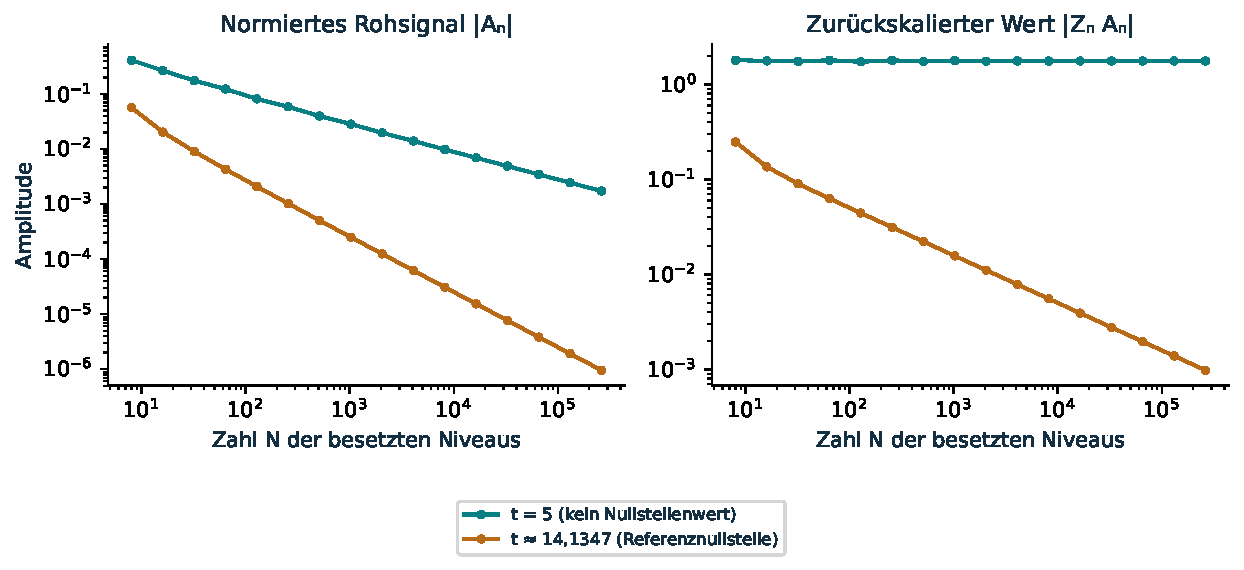
\includegraphics[width=\linewidth]{figures/shadow_eta_normalization.pdf}
\caption{Eigene endliche Rechnung für $\beta=1/2$. Links verschwinden beide Rohsignale. Rechts trennt die Rückskalierung einen gewöhnlichen Wert von der Umgebung der ersten bekannten Nullstelle. Die Kurven sind Formelauswertungen, keine Messdaten und kein Nullstellenzertifikat.}
\end{figure}

Um die zurückskalierte Amplitude mit absolutem Fehler $\varepsilon$ zu bestimmen, muss der Rohfehler von Größenordnung $\varepsilon/Z_N$ sein. Bei gewöhnlichen unabhängigen Messungen beschränkter Observablen führt die übliche Stichprobenschranke zu einem Aufwand $O(Z_N^2/\varepsilon^2)$ für feste Konfidenz. Bei $\beta=1/2$ wächst dieser wie $O(N/\varepsilon^2)$. Für $N=2^q$ ist das exponentiell in den Registerbits $q$. Dies ist eine Kostenrechnung für \emph{diesen Messweg}, keine allgemeine Quantenuntergrenze und keine Widerlegung der zwei vollständigen Protokolle von F06. Kohärente Amplitudenschätzung, andere Normierungen und gekoppelte Grenzwerte müssen jeweils separat bilanziert werden.

Der konkrete Gewinn für unser Puzzle lautet: \emph{Die Zustandsnormierung gehört zur physikalischen Bedeutung eines arithmetischen Schattens.} Registergröße, Präparation, Präzision, Messwiederholungen und Grenzwert dürfen nicht hinter einer eindrucksvollen Nullstelle verschwinden.

\chapter{Was Quantenphänomene über den verborgenen Aufbau sagen}
\label{ch:shadow-quantum}
\begin{bild}{Nicht nur die Anzahl der Kugeln zählt}
Zwei Kästen können dieselben möglichen Messergebnisse enthalten und doch verschieden reagieren, wenn wir zuerst an einer anderen Stelle messen oder zwei Teile zusammenführen. Die Quantenphänomene sagen uns deshalb vor allem etwas über die Regeln des Zusammensetzens, über relative Phasen und über erlaubte Eingriffe. Genau diese Daten verliert ein einfacher Schatten leicht.
\end{bild}

\section{Interferenz verlangt eine Information vor den Wahrscheinlichkeiten}
Für zwei Alternativen mit Amplituden $a$ und $b$ lautet die Born-Regel
\[
 P_{ab}=|a+b|^2=|a|^2+|b|^2+2\Re(a\bar b).
\]
Der letzte Term kann verstärken oder auslöschen. Wer ausschließlich die beiden Einzelwahrscheinlichkeiten aufbewahrt, kann ihn nicht rekonstruieren. Das erklärt im Kleinen, warum die behaltenen Register und Echoexperimente der früheren Kapitel mehr verraten als der erste sichtbare Markovschritt.

Für drei unter denselben idealen Bedingungen zusammengesetzte Alternativen gilt exakt
\begin{equation}
 I_3=P_{abc}-P_{ab}-P_{ac}-P_{bc}+P_a+P_b+P_c=0.
\end{equation}
Dies ist die algebraische Folge der quadratischen Born-Regel, hier für beliebige komplexe $a,b,c$ symbolisch kontrolliert. Dreispaltexperimente begrenzen Abweichungen von dieser Vorhersage; die reale Änderung der Randbedingungen beim Öffnen eines Spalts muss in der Auswertung berücksichtigt werden. Eine endliche Fehlerschranke beweist keine absolut exakte Null in der Natur. \src{F08}

\textbf{Constraint für den Universalraum:} Ein Modell muss Phasen vor der Wahrscheinlichkeitsbildung tragen, ihre Zusammensetzung erklären und die beobachtete Interferenzordnung reproduzieren. Es reicht nicht, die Born-Regel nachträglich als Ausleseformel einzusetzen und damit ihre Herkunft als gelöst zu bezeichnen.

\section{Der vorhandene Baukasten enthält bereits Kontextualität}
Die 15 Zwei-Qubit-Pauli-Kontexte der Synthese enthalten das folgende Mermin--Peres-Quadrat. Hier bedeutet $XI=X\otimes I$ und entsprechend für die anderen Einträge:
\begin{figure}[H]\centering
\begin{tikzpicture}[x=2.25cm,y=1.05cm]
\foreach \x/\y/\t in {0/2/XI,1/2/IX,2/2/XX,0/1/IZ,1/1/ZI,2/1/ZZ,0/0/XZ,1/0/ZX,2/0/YY}
 {\node[box,minimum width=18mm,minimum height=8mm] at (\x,\y) {$\t$};}
\foreach \y in {0,1,2}{\node[text=teal,font=\sffamily] at (3.1,\y) {Produkt $+I$};}
\node[text=teal] at (0,-.9) {$+I$};\node[text=teal] at (1,-.9) {$+I$};\node[text=amber] at (2,-.9) {$-I$};
\node[font=\sffamily\small,text=slate] at (1.1,-1.6) {Spaltenprodukte: genau ein Minuszeichen};
\end{tikzpicture}
\caption{Jede Zeile und jede Spalte ist gemeinsam messbar. Alle Zeilenprodukte sind positiv, aber das letzte Spaltenprodukt ist negativ. Diese sechs Kontexte gehören zum bereits verwendeten Pauli-System.}
\end{figure}

Angenommen, jede der neun Größen hätte vor der Messung einen festen, vom Kontext unabhängigen Wert $\pm1$, und diese Werte respektierten die Produktregel für gemeinsam messbare Größen. Multipliziert man alle sechs Kontextgleichungen, erscheint jeder Einzelwert zweimal: links muss $+1$ stehen. Die rechten Seiten ergeben aber $-1$. Das ist ein Widerspruch. Die neue Gegenrechnung prüft alle Operatorprodukte und zusätzlich sämtliche $2^9=512$ möglichen Wertzuweisungen. Keine erfüllt alle Bedingungen. \src{F09; eigener Nachbau}

Das Ergebnis ist \emph{zustandsunabhängig}; die Identitäten gelten als Operatorgleichungen. Es sagt nicht, dass jede klassische Simulation unmöglich sei. Der eingeschränkte Clifford-/Stabilizer-Baukasten kann effizient simulierbar sein und trotzdem diese naive, kontextunabhängige Wertvorstellung ausschließen. Auch der passive 60-Zustands-Prozess ist kein Gegenbeweis gegen Kontextualität: Er verfolgt nicht automatisch alle Eingriffe mit einer einheitlichen vorab festgelegten Wertzuweisung.

\textbf{Folgerung:} Die reichere Struktur muss mindestens Messkontexte und ihre gemeinsamen Observablen bewahren. Die bloße Liste möglicher Ergebnisse, ihre Anzahl 60 oder eine stationäre Verteilung bewahrt zu wenig. Damit erhält die im Buch geforderte Algebra der erlaubten Operationen einen sehr konkreten Grund.

\section{Verschränkung legt die Zusammensetzung fest}
\begin{grenze}{Integrierte Grenze v1.6: einfach bedeutet nicht quadratisch}
Für jeden der 60 nativen hellen Zweifermionenzustände ergibt ein passendes besetztes Modenpaar $\langle n_i n_j\rangle=1/8$, während ein Gauß-Zustand mit denselben Zweipunktdaten nur $1/64$ liefern würde. Die exakte Differenz $7/64$ ist frisch für alle 60 Kanäle geprüft. Damit ist der betreffende Zustand in den physischen Fermionmoden nicht gaußsch. Eine andere, nichtlineare Randfeldbeschreibung bleibt möglich, benötigt aber ihre konkrete Übersetzungsregel. Eine Majorana-Zweipunktfunktion allein ersetzt weder dieses Vierpunktdatum noch den nativen Wechselwirkungsoperator.
\end{grenze}


Für zwei räumlich getrennte Messstellen hat die CHSH-Kombination
\[
 S=\langle A_0B_0\rangle+\langle A_0B_1\rangle
 +\langle A_1B_0\rangle-\langle A_1B_1\rangle
\]
in einem lokalen Modell mit unabhängiger Wahl der Einstellungen die Grenze $|S|\leq2$. Quantenmechanik erreicht $2\sqrt2$. Mit $A_0=Z$, $A_1=X$ und $B_{0,1}=(Z\pm X)/\sqrt2$ ist der zugehörige Operator $\sqrt2(ZZ+XX)$; seine Eigenwerte sind $-2\sqrt2,0,0,2\sqrt2$. Beides wurde hier exakt nachgerechnet. Bell-Experimente prüfen solche Unterschiede unter sorgfältig formulierten Bedingungen. \src{F07}

Kein nutzbares Überlichtsignal folgt aus einer Verletzung. Umgekehrt reicht die Forderung \glqq kein Signal\grqq{} allein nicht zur Quantenmechanik: Allgemeine nichtsignalisierende Korrelationen können den algebraischen Wert 4 erreichen. Die gesuchte Struktur muss daher mehr auswählen als bloße Nichtsignalisierung. Sie muss die spezielle quantenmechanische Menge gemeinsam möglicher Korrelationen reproduzieren.

Für die TFPT-Zellen bedeutet dies: Die lokale Dimension 4 und ein singulärer Vierträgerzustand liefern geeignete endliche Zutaten. Dass entfernte physikalische Zellen tatsächlich die richtigen lokalen Messalgebren, Einstellungen und Korrelationen besitzen, bleibt ein zusätzlicher dynamischer und räumlicher Nachweis. Das algebraische Beispiel ist noch kein Bell-Experiment an TFPT-Materie.

\section{Gleiche Energien können verschiedene Welten beschreiben}
Wähle bei festgehaltenen Labor-Teilsystemen
\[
 H_0=Z\otimes I+2I\otimes Z,
 \quad U=\mathrm{CNOT}(H_{\mathrm{Had}}\otimes I),
 \quad H_1=UH_0U^\dagger.
\]
Beide Hamiltonoperatoren haben exakt die Energien $-3,-1,1,3$. Der Grundzustand von $H_0$ ist ein Produktzustand, der von $H_1$ ein Bell-Zustand. Die Reinheit $\Tr\rho_A^2$ eines lokalen Teils beträgt entsprechend 1 beziehungsweise $1/2$.

\begin{figure}[H]\centering
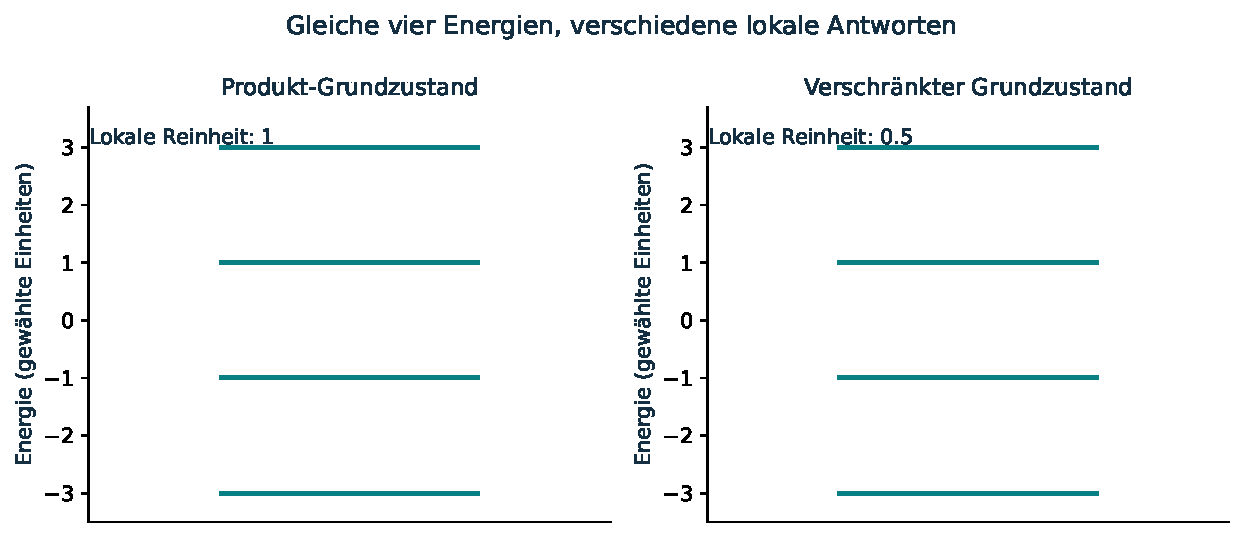
\includegraphics[width=\linewidth]{figures/shadow_isospectral.pdf}
\caption{Eine Liste von Energien erkennt die lokale Verschränkung nicht. Hier bleiben die Laboralgebren fest; würden auch alle Observablen mittransformiert, wäre es nur ein Darstellungswechsel.}
\end{figure}

Diese Gegenprobe verdichtet die Spektralfrage des RH-Zweigs: Selbst eine exakte Liste richtiger Eigenwerte bestimmt die physikalische Lokalität und die messbaren Antworten noch nicht. Dazu gehören Eigenvektoren relativ zu einer beobachtbaren Algebra und gemischte Korrelationsfunktionen. Die Zuordnung eines Tensorprodukts ist selbst durch die verfügbaren Observablen bestimmt. \src{E10; eigene Rechnung}

\section{Was komplexe Zahlen verraten und was offenbleibt}
Die komplexe Vierdimensionalität ist für den bestehenden Pauli-/Spinorbaukasten passend. Eine direkte Ableitung der komplexen Zahlen aus einem einzelnen Quantenphänomen wäre trotzdem zu stark. Renou und Mitautoren untersuchen Quantennetzwerke, in denen die übliche reale und komplexe Theorie unter einer bestimmten Unabhängigkeits- und Kompositionsannahme verschiedene Vorhersagen machen. \src{F10}

Eine Arbeit von Hoffreumon und Woods aus März 2026 unterscheidet operative Unabhängigkeit von einer faktorisierenden mathematischen Beschreibung und formuliert einen realen Simulationsrahmen. Ein Kommentar vom April diskutiert wiederum die Verträglichkeit vorgeschlagener Prinzipien mit fermionischer Informationstheorie. Diese neuen Arbeiten werden hier als fachliche Debatte eingeordnet, nicht als endgültige Entscheidung über die Natur der Zahlen. \src{F11, F12}

Die belastbare Verdichtung lautet: \emph{Experimentell bedeutsam ist das gemeinsame Paket aus Zustandsraum, erlaubten Operationen, Zusammensetzung und Unabhängigkeit.} Ein Wechsel von $\C$ nach $\R$ bei gleichzeitig veränderter Zusammensetzungsregel ist kein bloßer Austausch eines Symbols. Unsere Universalraum-Hypothese muss genau dieses Paket auswählen.

\section{Messung, Zeitpfeil und Statistik}
Die bisherigen Registerbeispiele erklären, wie ein global kohärenter Ablauf nach eingeschränktem Zugriff wie ein irreversibler Prozess aussehen kann. Sie liefern noch keine eindeutige Lösung des Messproblems: Insbesondere folgt aus einer diagonalen reduzierten Dichtematrix allein keine Auswahl eines einzelnen Ereignisses. Eine zusätzliche Kollapsdynamik müsste messbare Abweichungen angeben; eine unitäre Beschreibung müsste die Rolle stabiler Aufzeichnungen und der verwendeten Wahrscheinlichkeiten klären.

Ebenso ist eine nichttriviale Phase nicht automatisch Wärmeproduktion. Eine ideale unitäre Phasenoperation ist reversibel. Thermodynamische Löschkosten betreffen konkrete Ressourcen und Zugriffsmöglichkeiten; bei Quantenspeicher kann sogar die bedingte Entropie negativ sein, ohne dass die globale Entropiebilanz verletzt wird. \src{F13}

Auch Bosonen und Fermionen entstehen nicht allein dadurch, dass eine Wurzelsumme fehlt. Die Austauschstatistik verlangt Mehrteilchenzustände und deren Austauschoperationen; ein Spin-Statistik-Satz verwendet weitere Voraussetzungen wie relativistische Lokalität und Positivität. Die \glqq harte Hülle\grqq{} aus dem Ursprungsteil bleibt daher eine klar benannte zusätzliche Regel. Sie gewinnt durch das Wort Quantenphänomen keine neue Herleitung.

\chapter{Drei Raumrichtungen und eine Zeit: Welche Bedingungen bleiben?}
\label{ch:shadow-dimension}
\begin{bild}{Dimension ist die Antwort auf eine Frage}
Eine Ameise auf einer dünnen Schnur kann entlang einer Richtung laufen. Auf einem Blatt kann sie außerdem ausweichen. In einem Zimmer kann sie auch über ein Hindernis hinweg. Eine Dimension zählt solche unabhängigen Möglichkeiten. Die Zahl der inneren Zustandskomponenten oder der Knöpfe eines Geräts ist etwas anderes.
\end{bild}

Unsere gewöhnliche makroskopische Beschreibung benötigt drei Raumkoordinaten und eine Zeitkoordinate. Das ist die Zielstruktur im beobachteten Gültigkeitsbereich, kein Beweis, dass bei jeder denkbaren Skala ausschließlich vier kontinuierliche Koordinaten fundamental existieren. Ein $E_8$-Rang 8, vier interne Zustände und eine dreidimensionale räumliche Ausbreitung zählen jeweils andere Dinge.

\section{Drei unterschiedliche Hinweise führen zur Zahl drei}
Ein traceloses hermitesches $2\times2$-Objekt hat genau drei reelle Komponenten:
\[
 h=x\sigma_x+y\sigma_y+z\sigma_z.
\]
Ergänzt man $tI$, ergibt die Determinante
\[
 \det(tI+h)=t^2-x^2-y^2-z^2.
\]
Der positive Kegel erfüllt $t\geq\sqrt{x^2+y^2+z^2}$. Das ist die präzise Lorentz-Brücke aus dem Ursprungsteil. Sie zeigt eine passende lokale algebraische Form. Noch fehlen ihre Interpretation als Ereignisse, die Verklebung zu einer Raumzeit und die richtige Dynamik.

Ein zweiter Hinweis ist ein generisches Zweibandmodell $H(k)=d_0(k)I+\sum_{a=1}^3d_a(k)\sigma_a$. Eine Entartung benötigt drei Gleichungen $d_1=d_2=d_3=0$. In einem dreidimensionalen Impulsraum kann sie deshalb isoliert und bei geeigneter topologischer Ladung stabil sein. Die Wahl eines Zweibandsektors und eines geeigneten kontinuierlichen Impulsraums wird dabei schon vorausgesetzt. Andere Symmetrien können diese Zählung verändern. \src{E11, E12}

Ein dritter Hinweis kommt aus Ausbreitung. Wenn eine Anregung bei langen Wellen in drei unabhängigen Richtungen propagiert, sollten Zustandsdichte, Wärmeausbreitung und Fernkorrelationen dieselbe Dimension anzeigen. Erst die Übereinstimmung dieser operational verschiedenen Bestimmungen wäre ein stärkerer Befund als eine einzelne passende Matrix.

\section{Eine neue Gegenprobe am Clebsch-Vorschlag}
Für einen Graph-Laplaceoperator $L$ definieren wir die mittlere Rückkehrfunktion und eine skalenabhängige Dimension durch
\begin{equation}
 P(\tau)=\frac1{|V|}\Tr e^{-\tau L},\qquad
 d_s(\tau)=-2\frac{d\log P(\tau)}{d\log\tau}.
\end{equation}
Auf einem großen regelmäßigen dreidimensionalen Gitter entsteht zwischen der Gitter- und der endlichen Systemskala ein Bereich mit $P(\tau)\sim\tau^{-3/2}$, also $d_s\approx3$. Bei einem endlichen zusammenhängenden Graphen geht $d_s$ sowohl für sehr kleine als auch sehr große $\tau$ gegen null. Deshalb ist ein \emph{ausgedehnter Zwischenbereich mit kontrollierter Vergrößerung} relevant.

Der Clebsch-Graph besitzt für $L=5I-A$ die Eigenwerte $0,4,8$ mit Vielfachheiten $1,10,5$. Somit gilt exakt
\[
 P_{\mathrm{Cl}}(\tau)=\frac{1+10e^{-4\tau}+5e^{-8\tau}}{16}.
\]
Eine einzelne solche Kurve liefert keine makroskopische dreidimensionale Geometrie. Die folgende Vergleichsrechnung zeigt, wie eine richtige Größenfamilie aussehen müsste.

\begin{figure}[H]\centering
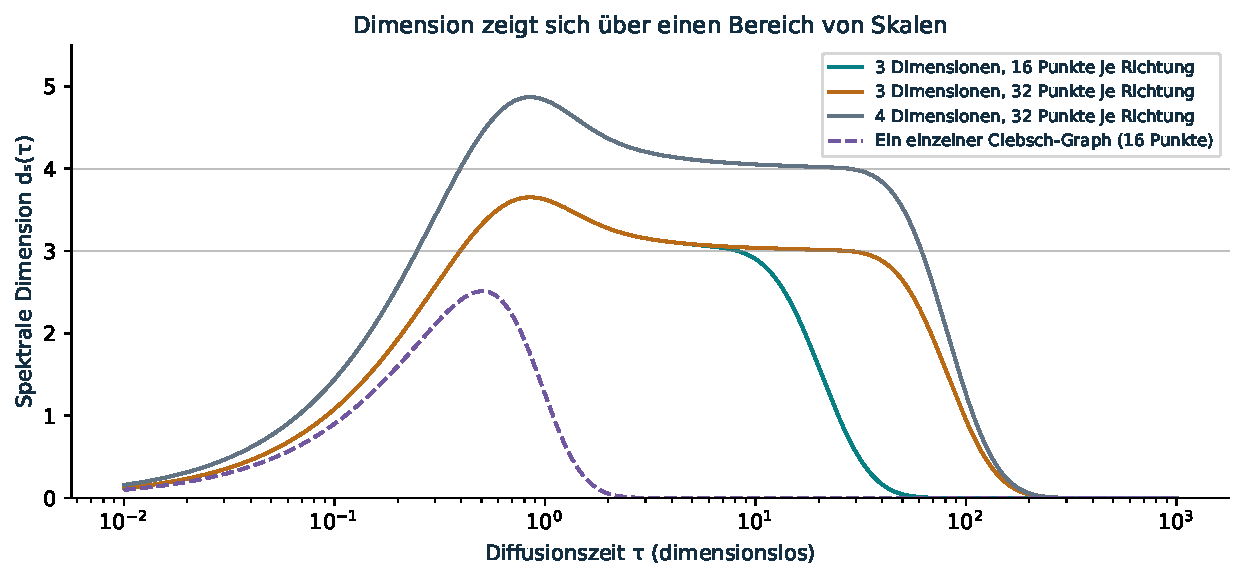
\includegraphics[width=\linewidth]{figures/shadow_dimension.pdf}
\caption{Eigene Wärmeausbreitungsrechnung. Regelmäßige periodische Gitter zeigen einen Bereich nahe ihrer eingesetzten Dimension; der Einzel-Clebsch-Graph besitzt keine daraus abgeleitete dreidimensionale Skalenfamilie. Der vierdimensionale Vergleich ist euklidisch und zählt keine Lorentz-Zeit.}
\end{figure}

Die Gitter sind hier bewusst eingesetzte Kontrollbeispiele. Ihre Dimension wurde nicht aus TFPT gewonnen. Ein nächster nativer Test müsste eine \emph{aus derselben Quelle erzeugte} wachsende Zellfamilie, deren Kopplungen und die passende Diffusions- oder Anregungsdynamik verwenden. Ein punktuelles Kreuzen von $d_s=3$ genügt nicht.

\begin{grenze}{Stärkere Gegenprobe v1.3}
Vier periodische Überlagerungen besitzen dieselbe lokale Clebsch-Inzidenz in $d=1,2,3,4$ und jeweils eine positive quadratische akustische Form. Selbst diese Ausbreitungsbedingung wählt daher nicht drei Raumdimensionen. Das ist ein exaktes Gegenmodell gegen einen Auswahlschluss, kein Weyl- oder Raumzeitnachweis. Details: Kapitel~\ref{ch:audit13}.
\end{grenze}
\section{Eine Zeitrichtung ist mehr als ein weiterer Zahlenplatz}
In einer gewöhnlichen hyperbolischen Wellengleichung werden lokale Anfangsdaten auf einer räumlichen Fläche vorgegeben und entlang einer ausgezeichneten Zeitrichtung entwickelt. Mehrere Zeitkoordinaten verändern das Anfangswertproblem grundlegend. Unter zusätzlichen nichtlokalen Beschränkungen existieren dennoch wohldefinierte Mehrzeit-Probleme; ein pauschaler Unmöglichkeitssatz wäre falsch. \src{F14}

Für unseren Ansatz entsteht deshalb eine konkrete Auswahlaufgabe: Aus der Quelle müssen ein geeigneter Kausalkegel, erlaubte Anfangsdaten, stabile Evolution und eine konsistente lokale Energiebedingung hervorgehen. Der innere modulare Fluss einer Dichtematrix, der arithmetische $\log n$-Fluss und die im Labor gemessene Zeit sind zunächst drei verschiedene Konstruktionen. Ihre Gleichsetzung braucht einen eigenen Satz oder ein operationales Vergleichsexperiment.

\section{Was Stabilität zusätzlich einschränkt}
Ein elementares mechanisches Beispiel illustriert die Rolle von Constraints. Nimmt man in $d>2$ Raumdimensionen eine Newtonsche Punktkraft mit Gaußgesetz an, lautet das effektive Radialpotential
\[
 V_{\mathrm{eff}}(r)=\frac{\ell^2}{2mr^2}-\frac{k}{(d-2)r^{d-2}}.
\]
An einer Kreisbahn ergibt sich
\[
 V_{\mathrm{eff}}''(r_0)=\frac{(4-d)\ell^2}{mr_0^4}.
\]
Unter diesen Voraussetzungen sind solche Kreisbahnen bei $d=3$ stabil, bei $d>4$ instabil und bei $d=4$ in dieser Näherung marginal. Das ist eine eigene ausgeschriebene Modellrechnung, kein universeller Dimensionsbeweis: $d=2$ verwendet ein logarithmisches Potential; andere Kräfte und Dynamiken verändern das Ergebnis.

\textbf{Die gemeinsame Schlussfolgerung:} Drei Raumdimensionen werden plausibler, wenn lokale Matrixstruktur, stabile Anregungen, Ausbreitung und makroskopische Stabilität zusammenpassen. Keine der einzelnen Beobachtungen erzwingt bereits die ganze Auswahl. Der noch fehlende Schritt liegt in ihrer gemeinsamen Herkunft und im kontrollierten Skalenübergang.

\section{Integrierte Schlussfolgerung v1.6: drei innere Richtungen sind kein Dimensionsbeweis}
Die neue Eingabe verbindet $\mu_4$, eine zweidimensionale komplexe Darstellung, drei Pauli-Richtungen und eine räumliche Dreidimensionalität. Diese Kette enthält zusätzliche Voraussetzungen: Die komplexen irreduziblen Darstellungen von $\mu_4$ selbst sind eindimensional. Für $\C^2$ braucht man weitere nichtkommutierende Operationen. Drei Pauli-Koeffizienten begrenzen nicht automatisch die Dimension ihres Ortsarguments. Ein regulärer isolierter Weyl-Punkt in einer zweibandigen Beschreibung ist ein präziser bedingter Test, keine Auswahl der ursprünglichen Raumdimension.

Die $A_3$-Fundamentalgewichte bilden tatsächlich ein Tetraeder in einem dreidimensionalen Gewichtsraum; seine Gewichts- und Wurzelgitter haben BCC- beziehungsweise FCC-Lesarten. Die neuen Prüfungen trennen diese exakte Geometrie von der Wahl physischer Nachbarschaften. Ein ausgewählter Lift in das volle $E_8$-Gitter muss zusätzlich Metrik, Grad, geschlossene Wege und native Operatorprodukte erhalten. Die hierfür gefundenen Hindernisse und der inzwischen positiv berechnete interne Walk-Baustein stehen in Kapitel~\ref{ch:v16-operations}.


\chapter{Schwer verstandene Phänomene als zusätzliche Prüfsteine}
\label{ch:shadow-open}
Offene Physik ist kein freier Platz, in den jede neue Idee hineinpasst. Sie ist oft durch viele bekannte Eigenschaften eng begrenzt. Der nützliche Schritt lautet deshalb: Welcher Teil des Phänomens ist beobachtet, welcher Mechanismus fehlt, und welche Antwort müsste unser Modell zusätzlich liefern?

\section{Dunkle Materie: unsichtbar heißt nicht frei wählbar}
Gravitationslinsen und die Verteilung sichtbarer Materie in kollidierenden Haufen liefern eine wichtige Beobachtung: Der aus der Gravitation erschlossene Beitrag muss nicht dem heißen sichtbaren Gas folgen. Die Bullet-Cluster-Analyse ist ein prominentes Beispiel. Sie identifiziert damit noch kein bestimmtes mikroskopisches Teilchen. Zusammen mit anderen kosmologischen Daten ist sie eine starke Anforderung an jede Erklärung. \src{F15; E16}

Im Universalraum könnte man an schwach auslesbare Sektoren denken. Das ist zunächst eine Hypothese. Der bloße Umstand, dass eine Komponente in einem Schatten unsichtbar bleibt, gibt ihr keine gravitative Wirkung, passende Dichte oder lange Lebensdauer. Ein konkreter Kandidat müsste gleichzeitig seine geringe elektromagnetische Kopplung, seine Gravitation, seine Entstehung und seine Verteilung erklären. Ein lokales Register, das ein Beobachter gerade nicht ausliest, ist deshalb nicht schon dunkle Materie.

\section{Dunkle Energie: ein kleiner Rest mit großen Folgen}
Die beschleunigte kosmische Expansion verlangt eine konsistente Erklärung im Gesamtmodell. Für TFPT ist besonders schwierig, eine passende effektive Vakuumwirkung zu erhalten, ohne sie bei jedem neuen Beitrag nachzujustieren. Der Mechanismus müsste seine Größe und Stabilität gegenüber Korrekturen erklären.

DESI DR2 untersucht unter anderem eine zeitabhängige Zustandsgleichung. Die Präferenz hängt von den kombinierten Datensätzen und dem gewählten Modell ab; sie ist nicht mit einer gesicherten Entdeckung dynamischer dunkler Energie gleichzusetzen. Der hier herangezogene Bericht ist die veröffentlichte DR2-Auswertung von 2025, im September 2026 geprüft. \src{F16}

Ein \glqq Informationsdruck\grqq{} des Universalraums würde erst dann etwas erklären, wenn ein wirksamer Energie-Impuls-Tensor folgt: mit Erhaltungsgesetz, Zustandsgleichung, stabilen Störungen und überprüfbarer Entwicklung. Ohne diesen Schritt bleibt das Wort ein Bild. Ebenso darf eine Spannung zwischen kosmologischen Messwegen nicht von vornherein als Beweis einer bestimmten neuen Dynamik behandelt werden.

\section{Schwarze Löcher: Information kann die Aufteilung selbst betreffen}
Die Schwarzlochfrage verbindet Quanteninformation, Gravitation und die Wahl zugänglicher Teilsysteme besonders eng. In bestimmten berechenbaren Modellen verändern Quanteneffekte die extremale Fläche und damit die Zuordnung rekonstruierbarer Information. Die verallgemeinerte Entropie enthält einen Flächenbeitrag und einen Quantenfeldbeitrag. Das ist erheblicher theoretischer Fortschritt in diesen Modellen, aber noch keine vollständige Beschreibung eines realistischen verdampfenden astrophysikalischen schwarzen Lochs. \src{F17}

Für die Universalraum-Idee ist daran interessant, dass der \emph{Zugang} zu Information von Geometrie und Dynamik abhängt. Das passt zur operationalen Definition von Schatten. Eine Ableitung müsste jedoch viel konkreter werden: Woher stammt ein Horizont, warum tritt ein Flächenterm auf, und welche Algebra ist jeweils zugänglich? Ein endliches Aufzeichnungsregister mit Entropie genügt nicht zur Herleitung der Bekenstein--Hawking-Beziehung.

\section{Gravitation muss sehr verschiedene Inhalte gleich behandeln}
Äquivalenztests wie MICROSCOPE prüfen die Universalität des freien Falls für unterschiedliche Materialien mit hoher Genauigkeit. Eine neue Quelle für Raumzeit muss daher erklären, warum verschiedene innere Zusammensetzungen auf dieselbe effektive Geometrie reagieren. \src{F18}

Ein gemeinsamer Kausalkegel ist dafür ein Anfang. Wenn aber jeder TFPT-Sektor seine eigenen Ausbreitungsgeschwindigkeiten oder seine eigene gravitative Kopplung behalten würde, wäre die allgemeine Universalität noch nicht gewonnen. Die Aufgabe lautet nicht nur, ein Spin-2-ähnliches Muster zu finden, sondern eine konsistente, universelle Kopplung mit den bekannten Niedrigenergiegrenzen zu erhalten.

\section{Weitere offene Stellen mit unterschiedlicher Beweiskraft}
\begin{longtable}{L{32mm}L{56mm}L{60mm}}
\toprule\textbf{Thema}&\textbf{Was den Ansatz einschränkt}&\textbf{Was eine Erklärung liefern müsste}\\\midrule\endhead
Zeitpfeil&Beständige Aufzeichnungen und irreversible Makroprozesse bei oft reversiblen Grundgleichungen.&Zustandsauswahl, Anfangskorrelationen, Zugriff und Entropiefluss; keine bloße Benennung eines inneren Parameters als Zeit.\\
Messproblem&Interferenz und stabile Messergebnisse müssen zusammen beschrieben werden.&Ein vollständiges Messmodell samt Wahrscheinlichkeiten oder eine abweichende Dynamik mit unterscheidbarer Vorhersage.\\
Massen und Familien&Gemessene Teilchenspektren und Mischungen, einschließlich Neutrino-Oszillationen.&Die Auswahl der Sektoren und ihrer Parameter mit Fehlerrechnung; passende kleine Zahlen allein reichen nicht.\\
Materieüberschuss&Die heutige Materie-Antimaterie-Asymmetrie verlangt eine kosmologische Entstehungsgeschichte.&Geeignete Symmetrieverletzung und Nichtgleichgewichtsdynamik mit quantitativer Ausbeute.\\
Starke CP-Frage&Im starken Sektor muss eine mögliche CP-verletzende Wirkung sehr klein sein.&Einen Schutz- oder Auswahlmechanismus samt Konsequenzen; ein Vorzeichenmuster im internen Gitter ist noch kein solcher Mechanismus.\\
Quantenfelder und Gravitation&Quantenwahrscheinlichkeiten, Lokalität und die erfolgreichen klassischen Näherungen müssen vereinbar bleiben.&Eine gemeinsame Dynamik mit kontrollierten Grenzwerten und experimentell zugänglichen Abweichungen.\\\bottomrule
\end{longtable}
\src{Einordnung; quantitative Referenzdaten in E14--E16, zusätzliche Primärquellen F07--F19; F19: Neutron-Dipolmessung als CP-Prüfstein}

Diese Liste behauptet nicht, alle Probleme seien gleich unverstanden. Quantenmechanik besitzt extrem erfolgreiche Vorhersageregeln, obwohl ihre Interpretation diskutiert wird. Dunkle Materie hat eine starke beobachtete gravitative Rolle, obwohl ihre mikroskopische Natur offen ist. RH ist dagegen ein exakt formuliertes mathematisches Problem. Die verschiedenen Arten von Unwissen dürfen nicht zu einem einzigen scheinbaren Beleg verschmelzen.

\begin{bild}{Die verdichtete Lektion}
Ein gemeinsamer Ursprung wäre besonders überzeugend, wenn ein und dieselbe getroffene Wahl mehrere Aufgaben gleichzeitig löst: etwa lokale Quantenkorrelationen, stabile Ausbreitung und eine bestimmte arithmetische Spur. Ein neues freies Einstellrad pro Phänomen würde den gemeinsamen Ursprung noch nicht erklären.
\end{bild}

\chapter{Ein engeres Bild und ein neues berechenbares Puzzleteil}
\label{ch:shadow-synthesis}
Die zusammengetragenen Schatten sprechen am stärksten für eine Struktur von \emph{Zusammensetzungen und gemeinsamen Antworten}. Arithmetik verlangt eindeutig kombinierbare primitive Faktoren. Quantenphänomene verlangen Phasen, Kontexte und eine besondere Zusammensetzung von Teilsystemen. Raumzeit verlangt eine skalenstabile Ordnung von Nachbarschaften, Signalwegen und Anfangsdaten. Keine dieser Forderungen wird durch die Zahl der anderen automatisch erfüllt.

\begin{grenze}{Versionsgrenze der arithmetischen Fortsetzung}
Die folgenden Prim-/Pauli-Modelle und RH-Einordnungen sind der bewahrte Stand v1.1. Die neue gemeinsame Ausführung vereinigt einen endlichen Zell-, Register- und Präparationsprozess, nicht diese arithmetische Zuordnung. Ihre Verbindung, ein RH-Beweis, effiziente Faktorisierung oder P=NP folgt daraus nicht.
\end{grenze}
\section{Eine engere Arbeitshypothese}
Die bildhafte Aussage \glqq Alles ist aus Primzahlen gebaut\grqq{} lässt sich zu einer brauchbareren Hypothese präzisieren:
\begin{quote}
Ein möglicher gemeinsamer Ursprung besitzt elementare, zusammensetzbare Operationen. In einem kommutativen arithmetischen Schatten erscheinen primitive Faktoren. Vor dieser Auslesung bleiben zusätzliche Phasen, Kontexte und Aufzeichnungen erhalten. Räumliche Nachbarschaft und Zeitordnung müssten aus den erlaubten gemeinsamen Operationen entstehen.
\end{quote}
\status{Hypothese.} Diese Formulierung identifiziert Primzahlen mit einer Art primitiver \emph{Zusammensetzbarkeit}, nicht mit einer festgelegten Liste von Elementarteilchen. Sie ist enger als ein beliebiges \glqq alles hängt zusammen\grqq{}, weil sie konkrete Relationen und gemischte Antworten verlangt. Sie bleibt weiter als ein eindeutiges fertiges Modell.

Formal bietet sich eine Algebra von Operationswörtern mit einem positiven normierten Funktional $\omega$ an. Für Wörter $w_i$ muss
\[
 M_{ij}=\omega(w_i^\dagger w_j)\succeq0,\qquad\omega(1)=1
\]
gelten. Daraus lässt sich eine Hilbertraumdarstellung rekonstruieren. Die Wahl der Wortrelationen, des Zustands und des physikalischen Zugriffs wird dadurch noch nicht erklärt. Insbesondere muss das signierte arithmetische Funktional erst mit dem passenden Objekt \emph{identifiziert} werden; ein beliebiges positives $M$ erfüllt RH nicht.

\section{Ein konstruktiver Versuch: gleiche Zahl, verschiedene Phasen}
Die folgenden Formeln sind eine neue Anschlusskonstruktion für dieses Buch. Ihre Zutaten sind Standardoperatoren; sie beanspruchen keine neue allgemeine mathematische Entdeckung. Sie zeigen jedoch exakt, dass ein gemeinsamer arithmetischer Endpunkt unterschiedliche kohärente Geschichten besitzen kann.

Wir nehmen den Raum $\ell^2(\mathbb N_{>0})\otimes\C^4$. Der erste Faktor besitzt Basiszustände $\ket n$, der zweite ist der bereits bekannte Zwei-Qubit-Raum. Definiere
\[
 S_m\ket n=\ket{mn},\qquad H_{\mathrm{ar}}\ket n=(\log n)\ket n.
\]
Die $S_m$ sind Isometrien und erfüllen $S_mS_n=S_{mn}$. Auf dem natürlichen Definitionsbereich gilt
\[
 [H_{\mathrm{ar}},S_m]=(\log m)S_m,
 \qquad e^{itH_{\mathrm{ar}}}S_me^{-itH_{\mathrm{ar}}}=m^{it}S_m.
\]
Der unbeschränkte logarithmische Generator ist hier ausdrücklich eingesetzt. Diese Konstruktion umgeht nicht das Hindernis eines endlichen festen Uhralphabets; sie verwendet dessen Voraussetzung gar nicht.

Nun heften wir an die Multiplikation mit 2 und 3 zwei vorhandene lokale Operationen:
\begin{equation}
 \widetilde S_2=S_2\otimes(X\otimes I),\qquad
 \widetilde S_3=S_3\otimes(Z\otimes I).
\end{equation}
Da $XZ=-ZX$, gilt
\begin{equation}
 \widetilde S_2\widetilde S_3=-\widetilde S_3\widetilde S_2.
 \label{eq:arithmetic-projective}
\end{equation}
Die beiden Wege $1\to2\to6$ und $1\to3\to6$ führen zum gleichen Zahlzustand und, einzeln betrachtet, zum gleichen lokalen Strahl. Der Unterschied ist eine relative Phase von $-1$. Eine reine Endpunktzählung sieht ihn nicht.

\begin{figure}[H]\centering
\begin{tikzpicture}[x=1cm,y=1cm]
\node[box] (one) at (0,0) {$1,\ \ket\psi$};
\node[box] (two) at (4,1.4) {$2,\ X\ket\psi$};
\node[box] (three) at (4,-1.4) {$3,\ Z\ket\psi$};
\node[box,text width=29mm] (six) at (8,0) {$6$\\gleicher Strahl};
\draw[arr] (one)--node[above left,font=\small] {$\times2,\ X$}(two);
\draw[arr] (one)--node[below left,font=\small] {$\times3,\ Z$}(three);
\draw[arr] (two)--node[above right,font=\small] {$\times3,\ Z$}(six);
\draw[arr] (three)--node[below right,font=\small] {$\times2,\ X$}(six);
\node[openbox,text width=105mm] at (4,-3.1) {Kohärentes Zusammenführen sieht das Minuszeichen.\\Unabhängige Endpunktmessungen verlieren es.};
\end{tikzpicture}
\caption{Ein arithmetischer Schatten mit nichttrivialer Quantenphase. Die Auswahl $2\mapsto X$, $3\mapsto Z$ ist gesetzt. Die daraus folgende Wegabhängigkeit ist exakt.}
\end{figure}

\subsection{Eine vollständig bestimmte Vorhersage im Modell}
Ein Kontrollqubit speichert kohärent, welcher der beiden Wege durchlaufen wurde. Setze $w_0=\widetilde S_2\widetilde S_3\ket{1,\psi}$ und $w_1=\widetilde S_3\widetilde S_2\ket{1,\psi}=-w_0$. Nach einer Hadamard-Auslesung des Kontrollqubits gelten
\[
 P_+=\tfrac14\|w_0+w_1\|^2=0,
 \qquad P_-=\tfrac14\|w_0-w_1\|^2=1.
\]
Ohne die lokalen $X,Z$-Markierungen wäre $w_0=w_1$ und damit $P_+=1$. Die neue Rechnung kontrolliert dies im Zahlfenster $1\leq n\leq12$ exakt. Die benutzten Wege ab $n=1$ verlassen dieses Fenster nicht. Die abgeschnittenen $S_m$ sind außerhalb dieses ausgewählten Unterraums keine Isometrien; daraus wird keine globale endliche Unitarität behauptet. Eine reale Schaltung müsste die kontrollierten Isometrien mit zusätzlichen Registern reversibel realisieren und deren Kosten ausweisen.

\subsection{Was damit gelöst ist und was nicht}
Gelöst ist eine kleine \emph{Kompatibilitätsfrage}: Unbegrenzte arithmetische Zusammensetzung und ein endlicher lokaler Quantenbaukasten lassen sich in einem expliziten gemeinsamen Modell verbinden. Der rein arithmetische Schatten kann kommutativ sein, während kohärent zugängliche Wegrelationen eine nichttriviale Phase behalten. Das passt genau zum Motiv der vorherigen Echoexperimente.

Die Schleifenphase ist stärker als ein beliebiger Wechsel der lokalen Basis. Transformiert man Zustände und Operatoren an den Knoten konsistent, bleibt die zentrale relative Phase einer geschlossenen Vergleichsschleife erhalten. Sie verschwindet nicht dadurch, dass man einzelne Knoten neu beschriftet. Dagegen ist die globale Phase einer \emph{einzeln} durchlaufenen Geschichte nicht beobachtbar; der Interferenzvergleich ist wesentlich.

Offen bleiben die Auswahl der Primmarkierungen aus TFPT, eine kanonische Fortsetzung auf alle Primzahlen, der richtige gemeinsame Zustand und die physikalische Realisierung. Für allgemeine Primzahlen könnte man Pauli-Labels wählen; eine solche willkürliche Tabelle wäre aber gerade keine Herleitung. Ebenso liefert die Konstruktion weder die signierte Weil-Positivität noch drei Raumdimensionen, Gravitation oder einen Faktorisierungsgewinn.

\section{Warum getrennte passende Modelle noch keine gemeinsame Quelle sind}
Man könnte einen arithmetischen Raum, ein Quantensystem und ein geometrisches Modell einfach nebeneinanderstellen:
\[
 \mathcal H_{\mathrm{ar}}\otimes\mathcal H_{\mathrm{q}}\otimes\mathcal H_{\mathrm{geo}}.
\]
Bei Produktzustand und unabhängig wirkenden Operationen passen dann vielleicht alle Einzelstatistiken. Der gemeinsame Ursprung wäre dadurch nicht erklärt. Nötig sind gemeinsame Relationen und überprüfbare Antworten auf gemischte Eingriffe. Die oben konstruierte Wegphase ist ein kleines Beispiel einer solchen Antwort.

Eine weitere mögliche Diagnose ist $C(A,B)=\omega(AB)-\omega(A)\omega(B)$ für festgelegte Observablen aus zwei Sektoren. Ein nichtverschwindendes $C$ widerlegt deren einfache Produktbeschreibung in diesem Zustand. Ein einzelnes verschwindendes $C$ beweist umgekehrt keine vollständige Unabhängigkeit; dafür braucht man eine hinreichend vollständige Klasse von Tests. Auch Korrelation allein erklärt noch keine gemeinsame Herkunft der Gesetze.

\begin{figure}[H]\centering
\begin{tikzpicture}[node distance=8mm]
\node[box,text width=43mm] (a) {Arithmetische Sicht\\Faktoren, Spuren, alle Skalen};
\node[box,text width=43mm,right=24mm of a] (q) {Quantensicht\\Phasen, Kontexte, Register};
\node[openbox,text width=104mm,below=15mm of a.south east,anchor=north] (m) {Gemeinsame Operationsrelationen und gemischte Antworten\\Wegphase ist ein endliches Beispiel; native Auswahl bleibt offen};
\node[box,text width=104mm,below=12mm of m] (g) {Raumzeit und Makrophysik\\Nachbarschaft, Kausalität, stabile Dimension, universelle Kopplung};
\draw[arr] (a.south)--(m.north west);\draw[arr] (q.south)--(m.north east);\draw[hyp] (m)--(g);
\end{tikzpicture}
\caption{Die stärkere Universalraum-Hypothese sitzt in den gemeinsamen Beziehungen. Der gestrichelte Übergang zur Raumzeit verlangt weiterhin eine echte Ableitung.}
\end{figure}

\Needspace{140pt}
\section{Welche Puzzleteile jetzt enger gefasst sind}
\begin{longtable}{L{37mm}L{60mm}L{51mm}}
\toprule\textbf{Gewonnene Präzisierung}&\textbf{Konkretes Ergebnis}&\textbf{Nächste fehlende Bedingung}\\\midrule\endhead
Logarithmische Skala&Multiplikative Additivität plus Monotonie erzwingen $c\log n$.&Native Begründung der Ordnung und Energieskala.\\
Unbegrenzte Primfamilie&Endlich viele additive Grundtakte tragen nicht alle $\log p$.&Eine passende wachsende Familie oder reichere Dynamik.\\
Arithmetik und Phase&Zwei Multiplikationswege können eine messbare Schleifenphase behalten.&Die Prim-/Pauli-Markierung aus der Quelle auswählen.\\
Kontextualität&Das vorhandene Pauli-System besitzt den exakten Mermin-Widerspruch.&Physikalisch zugängliche Interventionen und Präparationen.\\
Spektrum und Raum&Gleiche Eigenwerte können verschiedene lokale Verschränkung tragen.&Gemeinsame Algebra, Zustandszuordnung und lokale Antworten.\\
Dimension&Eine skalierte Rückkehrfunktion liefert einen prüfbaren Dimensionsbegriff.&Native Größenfamilie mit stabilem Plateau und Ausbreitung.\\
RH und Positivität&Positive Einzelobjekte erzwingen kein positives signiertes Gesamtobjekt.&Exakte Identifikation, gemischte Kontrolle, sämtliche Tests und Ränder.\\
Experimenteller Zeta-Schatten&Kleine Rohamplitude kann allein aus wachsender Normierung folgen.&Kontrollierte Rückskalierung und vollständige Ressourcenrechnung.\\\bottomrule
\end{longtable}

Diese Fortsetzung schließt also mehrere kleine logische Lücken und liefert einen neuen endlichen Interferenztest. Sie schließt nicht die gesamte Theorie. Der aussichtsreichste nächste Schritt ist, für \emph{eine} native TFPT-Operationsfamilie die arithmetische Zusammensetzung und die kohärente Wegphase gemeinsam abzuleiten, anschließend die gemischte Antwort unabhängig zu berechnen und erst dann den Grenzwert auszubauen. Eine zusätzliche passende Zahl wäre weniger aussagekräftig als diese vollständig bestimmte Verbindung.

\chapter{Die sechs neuen Quellen: geprüfte Korrekturen}
\label{ch:audit13}
\section{Was gegenüber v1.1 neu ist}
Die sechs zusätzlichen Unterlagen heißen im neuen Quellenregister N1 bis N6; die ursprünglichen S01 bis S11 bleiben unverändert. Ihr Audit trennt exakte endliche Identitäten, numerische Spektren und zusätzliche Modellannahmen. 100 eigene Bedingungen bestanden: 78 exakte beziehungsweise Integritätsprüfungen und 22 numerische. Die anschließende gemeinsame Ausführung hat einen eigenen 231-Bedingungen-Vertrag. Diese Zählungen messen keine unabhängigen Entdeckungen.

\section{Die zentrale Reparatur: Wege nicht zu früh unterscheiden}
Setze $S\ket{ab}=\ket{ba}$ und $D=\sum_a\ket{aa}\bra{aa}$. Der Wedge-Kanal besitzt
\begin{equation}
K\ket{ab}=\ket{a\wedge b},\quad K\ket{ba}=-\ket{a\wedge b},\quad
K^\dagger K=I-S,\quad KK^\dagger=2I_6.
\end{equation}
Für $a=b$ verschwindet $K$. Beide geordneten Wege enden im gleichen virtuellen Zustand und interferieren. Orthogonale Records für $ab$ und $ba$ ersetzen dies durch $\widetilde K^\dagger\widetilde K=I-D$: Der antisymmetrische Rang-6-Kanal wird zum Rang-12-Kanal. Bei gleichem Energienenner entsteht eine Kollisionsenergie statt des gewünschten $\mathrm{SU}(4)$-Austauschs. Auf dem vollständigen Vierergraphen bleiben 24 Farbanordnungen im Grundraum; $\Omega$ ist nicht eindeutig.

Die Korrektur lautet $h_{e,ab}=h_{e,ba}$ innerhalb derselben Kante. Verschiedene Kanten dürfen durch Loch- und Zuschauerzustände unterscheidbar bleiben. Für reellen Überlapp $0\le\eta\le1$ lautet die interpolierende Gram-Matrix
\begin{equation}
G_\eta=I-\eta S-(1-\eta)D.
\end{equation}
Nach gemeinsamer Energieverschiebung erhält man
\begin{equation}
\overline H_\eta=2\eta H_{\mathrm{tet}}/J+(1-\eta)D_{\mathrm{coll}},
\qquad D_{\mathrm{coll}}=\sum_{i<j}D_{ij}.
\end{equation}
Für $\eta>0$ ist $\Omega$ eindeutig und die dimensionslose Lücke genau $4\eta$. Die untere Schranke folgt aus der Tetramerlücke und Positivität; sie wird im verschiedenen-Farben-Sektor erreicht. Führend entspricht dies $4\eta t^2/\Delta$. Bei $\eta=0$ springt die Kerndimension auf 24; die positive Lücke über dem gesamten Kern ist eins. Ein Elternoperator aus dem Projektor auf $\ker K_\eta$ wäre eine andere, diskontinuierliche Konstruktion.

\begin{bild}{Bildlich}
Zwei Wege dürfen ein gemeinsames Ziel erreichen, ohne ein unterscheidbares Wegschild zu hinterlassen. Dieses Schild würde ihre Interferenz zerstören. Aufzeichnen lässt sich stattdessen, ob ein Vermittlungsereignis stattfand. Diese gröbere Information verwendet die neue gemeinsame Ausführung.
\end{bild}

\section{Der erste Schatten wählt die Fortsetzung noch nicht}
Mit $P_\pm=(I\pm S)/2$ und $W=K/\sqrt2$ ist
\begin{equation}
U_\theta=\begin{pmatrix}e^{i\theta}P_+&W^\dagger\\W&0\end{pmatrix}
\end{equation}
auf $(\C^4\otimes\C^4)\oplus\C^6$ unitär und kollektiv $\mathrm{SU}(4)$-kovariant. Alle $\theta$ liefern für Materieeingänge denselben ersten blockdephasierten Schatten. Dennoch wirkt $U_0^2$ dort als $I$, während $U_{\pi/2}^2$ als $-S$ wirkt: $\ket{01}$ kehrt als $\ket{01}$ oder als $-\ket{10}$ zurück. Das Nullereignis unverändert zu lassen wählt $\theta=0$ in dieser Klasse, ist aber ein zusätzliches Prinzip.

\section{Der allkopplige Zweizellenbeweis}
Für genau zwei vollständige $K_4$-Zellen und eine positive Brücke gelten die Formeln aus Kapitel~\ref{ch:two} bei allen endlichen $\lambda\ge0$. Die lokalen Zellenergien sind $0,2J,3J,4J,6J$. Unter $4J$ können global nur das Produktsingulett, adjungierte Sektoren bei $2J$ und die 20 bei $3J$ auftreten. Der bekannte Singulettblock erreicht $E_0$; sein orthogonales Singulettkomplement beginnt bei mindestens $4J$.

Im adjungierten Sektor sei $P$ die $H_0$-Energie-$2J$-Projektion. Dann gilt $H_0\ge4JI-2JP$. Die exakt berechnete Kompression von $V=P^+_{ab}$ besitzt pro adjungierter Komponente
\begin{equation}
\spec(PVP|_{\operatorname{ran}P})
=\{(1/2)^{[1]},(5/8)^{[4]},(3/4)^{[1]}\}.
\end{equation}
Zum Eigenwert $p$ liefert der Zwei-Projektionen-Vergleich den unteren Wert
\begin{equation}
3J+\lambda/2-\tfrac12\sqrt{4J^2+4J\lambda(1-2p)+\lambda^2}.
\end{equation}
Wegen $p\ge1/2$ liegt dieser mindestens bei $E_1=3J+\lambda/2-\sqrt{4J^2+\lambda^2}/2$. Die Schranke wird im tatsächlich invarianten Block
\begin{equation}
\begin{pmatrix}2J+\lambda/2&\lambda/2\\\lambda/2&4J+\lambda/2\end{pmatrix}
\end{equation}
erreicht. Alle anderen Darstellungen beginnen bei mindestens $3J$, während $E_1<3J$. Mit $R$ und $Q$ aus Kapitel~\ref{ch:two} gilt
\begin{equation}
R^2-(Q-J)^2=11J^2+2J(Q-\lambda)>0,\quad Q-J>0.
\end{equation}
Also $R>Q-J$ und $E_1-E_0>J/2$. Der Grundzustand bleibt eindeutig. Für $\lambda\to\infty$ nähern sich $E_0$ und $E_1$ den Werten $5J/2$ und $3J$.

Ganzzahlige Tensoridentitäten wurden auf 65536 Komponenten geprüft; zusätzlich alle 15 zulässigen Youngsektoren bei zehn Kopplungswerten numerisch diagonalisiert. Der allgemeine Satz folgt aus dem Vergleichsbeweis, nicht aus diesen Stichproben. Eine größenuniforme Vielzellenlücke folgt nicht.

\section{Vierte Ordnung und unterschiedliche Subtraktionskonventionen}
Im ausgewiesenen harmonischen Modell eines geteilten Vermittlers lautet der symmetrische aktive Block
\begin{equation}
M_s=\begin{pmatrix}0&\sqrt2g&0\\\sqrt2g&\Delta&2g\\0&2g&2\Delta\end{pmatrix}.
\end{equation}
Sein niedriger Zweig beginnt mit $-2g^2/\Delta+O(g^6/\Delta^5)$; der antisymmetrische mit $-2g^2/\Delta+4g^4/\Delta^3+O(g^6/\Delta^5)$. Deshalb ist auf dem aktiven $6\otimes6$-Raum
\begin{equation}
H^{(4)}_{\mathrm{gesamt}}=4g^4P_-^{(6)}/\Delta^3.
\end{equation}
Nach Abzug beider Einzelbondkorrekturen $2g^4I/\Delta^3$ bleibt
\begin{equation}
H^{(4)}_{\mathrm{verbunden}}=-2g^4S_6/\Delta^3
=-8t^4S_6/\Delta^3,\quad g=\sqrt2t.
\end{equation}
Beide Schreibweisen sind kompatibel. Eine Konstante auf dem aktiven Sektor ist außerhalb davon nicht automatisch global skalar. Der vollständige Clebsch-Operator wurde in dieser früheren Auditstufe noch nicht geprüft. Die anschließenden neuen Eingaben und ihre Gegenprüfung in Kapitel~\ref{ch:newinputs13} erweitern genau diese Stelle.

Im isolierten Kanal ist $j=(\sqrt{\Delta^2+4g^2}-\Delta)/2$ exakt; $2t^2/\Delta$ ist nur führend. Das Verhältnis des verbundenen Koeffizienten zum führenden $J$ ist $4(t/\Delta)^2$: vier Prozent bei $t/\Delta=0{,}1$, ein Prozent bei $0{,}05$. Starker kohärenter Volltransfer ist kein Schwachkopplungsgrenzfall.

\section{Ein exakter Stern-Spektralfilter unter zusätzlichen Ressourcen}
Für $H_\star=J(P^+_{01}+P^+_{02}+P^+_{03})$ gilt
\begin{equation}
\spec(H_\star/J)=
\{0^{[1]},(1/2)^{[30]},1^{[45]},(3/2)^{[40]},2^{[15]},(5/2)^{[90]},3^{[35]}\}.
\end{equation}
Mit $M=2H_\star/J$ und $U=\exp[-i\pi H_\star/(2J)]$ folgen
\begin{equation}
\prod_{j=1}^{6}(jI-M)=720P_\Omega,\qquad
\frac18\sum_{k=0}^{7}U^k=P_\Omega.
\end{equation}
Ein kohärentes Achtzweigregister liefert aus dem früheren Zweisingulett-Eingang $\chi_0$ Erfolg $1/6$. Alle acht Ausgänge haben Gewichte $(1/6,1/6,0,0,1/6,1/6,1/6,1/6)$. Dies ist eine exakte Alternative zur alten 32-Zweigschaltung. Kontrollierte kontinuierliche Sternpulse und Register bleiben zusätzliche Ressourcen. Erzeugt man $\chi_0$ erst aus $\ket{0123}$ durch zwei Paarfilter, kostet das $1/4$; die Gesamtausbeute ist $1/24$.

\section{Einfachheit braucht einen Auslesevertrag}
In der Inzidenzfamilie $K_a$ sind die beiden relevanten Entropien
\begin{align}
H_C(a)&=-a\log a-(1-a)\log((1-a)/6),\\
H_R(a)&=-a\log a-(1-a)\log((1-a)/12).
\end{align}
Strikte Konkavität liefert verschiedene Maxima: $a=1/7$ für Kontexte und $a=1/13$ für Strahlen. Letzterer Prozess hat Rang 60. Erweitert man den Nachfolgerträger, entstehen symmetrieverträgliche Ränge 15 und 16. Weder maximale Entropie noch minimale Rangzahl wählt die Regel ohne erklärte Klasse. Die passive separate Marginalauslesung bleibt bei 45 linearen beziehungsweise 44 normierten affinen Größen; selektive Eingriffe gehören nicht dazu.

\section{Weitere architektonisch wichtige Korrekturen}
\begin{description}
\item[Clebsch.] Zwei Singulettläufe finden mindestens vier orthogonale Moden bei $11{,}561762122803J$ über $11{,}045398337068J$, Residuen unter $10^{-8}$. Das Dublett ist widerlegt; ein exakter oberer Multiplizitätsbeweis fehlt.
\item[$E_8$-Typen.] 960 gleichgradige Wurzelsummen gehen nach $(10,6)$; gemischt ergeben sich 640 und 192 Summen nach Grad null sowie 64 Cartanfälle. Der vorgeschlagene gemischte Kanal nach $(10,6)$ ist typwidrig. Die Korrektur schließt kein natives Half-Charge-Feld.
\item[Ort versus innere Symmetrie.] Im gewählten CAR-Modell liefert Gewichtsplatzmischung $[H_U,T]P=UTP\ne0$. Fester Gewichtsplatz als Ort und unverändert ungebrochene innere $\mathrm{Spin}(10)$-Mischung sind verschiedene Rollen.
\item[Kommutanten.] Die volle Kommutante eines einzelnen Tetramer-Hamiltonoperators hat Dimension $1^2+45^2+40^2+135^2+35^2=23076$. Rekonstruktion verlangt die gesamte lokale Operatorfamilie und deren erlaubte Automorphismen.
\item[Dimension.] Der Clebsch-Graph hat 16 Knoten, 40 Kanten und 25 unabhängige Zyklen. Mit reduzierter Inzidenzmatrix $D_\Gamma$ und Kantenspannungen $B_d$ wurde für vier periodische Überlagerungen in $d=1,2,3,4$ die akustische Form
\[
B_d^T[I-D_\Gamma(D_\Gamma^TD_\Gamma)^{-1}D_\Gamma^T]B_d/16
\]
rational positiv definit geprüft. Dieselbe lokale Inzidenz wählt daher keine Dimension.
\item[Weyl.] Richtig ist $\det(\omega I-\sum_i v_iq_i\sigma_i)=\omega^2-\sum_i v_i^2q_i^2$, ohne die falschen Kreuzterme einer voll summierten Form $v_iv_jq_iq_j$. Allgemein steht dort $\mathbf q^TV^TV\mathbf q$.
\item[Dunkler Zustand.] Für $L=I-P_\Omega$, $H=0$ ist jeder Zustand im orthogonalen Komplement stationär, obwohl der dunkle Raum nur $\C\Omega$ ist. Eindeutiger dunkler Vektor bedeutet nicht globaler Attraktor.
\end{description}
Alpha- und Inflationskorrekturen stehen integriert in Kapitel~\ref{ch:zahlen}. Negative Lepton-, Higgs- und Protonzweige bleiben erhalten. Kein RH-, Faktorisierungs-, P-vs-NP- oder TOE-Abschluss folgt aus dem Audit.

\chapter{Eine gemeinsame Ausführung für Record, Präparation und Mehrzeit}
\label{ch:execution13}
\begin{bild}{Aktualisierung v1.5: weniger zusätzliche Steuerung}
Die hier eingeführte gemeinsame Record-/Präparations-/Mehrzeitausführung lässt sich jetzt bei festem $\Delta>0$ ohne negative Evolutionszeiten anschließen. Endliche Q-Gatezeiten sind unter einem ausdrücklich belegungserhaltenden Gatevertrag mitgerechnet. Wedge-Kopplung, Q, adressiertes An/aus und Reset bleiben zusätzliche Ressourcen; Details in Kapitel~\ref{ch:execution15}.
\end{bild}
\section{Eine Konstruktion, aber ein ausdrücklich zusätzlicher Ressourcenvertrag}
Dieselbe korrigierte Vermittlungsoperation erzeugt jetzt Aufzeichnung, kontrollierte Näherungspräparation und Mehrzeitantwort. Die tatsächlichen Quellprojektoren, Paulioperationen und die Dreierclock wurden benutzt. Ein bereits präpariertes $\Omega$ oder ein separater Präparations-Hamiltonoperator wird nicht benötigt.

Gesetzt bleiben gekoppelte Träger, Wedge-Kopplung und ihre unitäre Fortsetzung, kohärenter Belegungszugriff, Registerinitialisierung und -messung, Kantensteuerung und Feedback. Die Messregel ist Voraussetzung. Die gemeinsame Konstruktion ist daher bedingt, nicht vollständig nativ.

\section{Die vollständige Recordoperation}
Mit $W^\dagger W=P_-$, $WW^\dagger=I_6$ und $WP_+=0$ gilt
\begin{equation}
U_0=\begin{pmatrix}P_+&W^\dagger\\W&0\end{pmatrix},\quad U_0^2=I_{22}.
\end{equation}
Kopiere nur die Vermittlerbelegung, nicht das geordnete Farbwort:
\begin{equation}
Q=I_{16}\otimes I_2\oplus I_6\otimes X.
\end{equation}
Dann ist auf allen 44 Dimensionen
\begin{equation}
(U_0\otimes I)Q(U_0\otimes I)
=(P_+\otimes I+P_-\otimes X)\oplus I_{12}.
\end{equation}
Der Vermittler kehrt zurück. Auf Materie und Pointer bleibt $R=P_+\otimes I+P_-\otimes X$, $R^2=I$, mit
\begin{equation}
R(\psi\otimes\ket0)=P_+\psi\otimes\ket0+P_-\psi\otimes\ket1.
\end{equation}
Beide Krausoperatoren gehören zum Instrument; ihre Effekte summieren sich zu $I$. Ein ungemessener Pointer bleibt kohärent.

\section{Ein gemeinsamer Träger und ein fester Schritt}
Für vier Materieträger und höchstens einen aktiven Vermittler sei
\begin{equation}
\mathcal H_{\mathrm{common}}=(\C^4)^{\otimes4}\oplus
\bigoplus_{e=1}^{6}(\C^6_e\otimes\C^4\otimes\C^4),\quad \dim=832.
\end{equation}
Alle sechs $W_e$ wurden auf dem vollen Materieraum rekonstruiert:
$W_e^\dagger W_e=P^-_e$, $W_eW_e^\dagger=I_{96}$, $W_eP^+_e=0$.
Andere Vermittlersektoren bleiben bei einer adressierten Operation unverändert. Die Kanten haben orthogonale Ausgänge; verschränkte Zuschauer sind eingeschlossen. Dies ist ein vollständiges sequenzielles Protokollmodell, kein Fockraum beliebig vieler aktiver Vermittler.

Die tatsächliche Clock $C$ permutiert $0\to1\to2\to0$ und fixiert 3. Sie erhält alle 240 phasenmarkierten Wurzeln und 60 Projektoren und normalisiert die Quell-Paulis. Mit $e(0)=01$, $e(1)=02$, $e(2)=03$ und $R_{e(3)}=I$ gilt
\begin{equation}
\mathbb U=(C\otimes I)\sum_{k=0}^{3}\ket k\bra k\otimes R_{e(k)}.
\end{equation}
Orthogonale Steuerblöcke machen $\mathbb U$ unitär. Mit Clock und Pointer hat der Raum Dimension 6656. Die Clock-Kanten-Zuordnung und das spätere Austauschen oder Auslesen der Pointer bleiben gesetzte Zugriffe. Eine physikalische Sekunde entsteht nicht aus der Dimensionszahl.

\section{Quellseitiger Reset ohne vorpräpariertes Zielreservoir}
Rechenbasis- und uniformer Projektor gehören zu den 60 tatsächlichen Quellprojektoren. Die Swap-Identität verwendet dieselben 16 Quell-Paulis:
\begin{equation}
S=\frac14\sum_{v=0}^{15}P_v\otimes P_v.
\end{equation}
Für Messausgang $x$ und Ziel $a$ liefert die Bitverschiebung
\begin{equation}
M_x=X_{a\oplus x}\ket x\bra x=\ket a\bra x,\quad
\sum_xM_x^\dagger M_x=I.
\end{equation}
Damit ist $\sum_xM_x\rho M_x^\dagger=\ket a\bra a\,\Tr\rho$. Vier lokale Resets erzeugen $v_0=\ket{0123}$ sogar aus verschränktem Eingang. Messung und Feedback bleiben Ressourcen, keine hergeleitete kosmologische Zustandswahl.

\section{Wiederholung präpariert den Viererzustand kontrolliert}
Akzeptiere in jeder Sternrunde die Recordfolge 111:
\begin{equation}
K_\star=P^-_{03}P^-_{02}P^-_{01},\quad v_N=K_\star^Nv_0,\quad p_N=\|v_N\|^2.
\end{equation}
Alle acht ersten Recordfolgen haben Wahrscheinlichkeit $1/8$. $\Omega$ wird erst zur Zielprüfung definiert. Im 24-dimensionalen Raum der verschiedenen Farbanordnungen gilt exakt
\begin{equation}
\det(xI-K_\star^\dagger K_\star)=
\frac{x^{12}(x-1)(16x-1)^5(16x^2-9x+1)^3}{2^{32}}.
\end{equation}
Dieser Raum trägt die treue reguläre Darstellung von $S_4$. Die polynomialen Identitäten der Gruppenalgebra gelten daher auch auf allen 256 Materiedimensionen. Die übrigen Eigenmultiplizitäten werden dabei nicht unverändert übernommen. Der Einsprojektor ist $P_\Omega$. Weil $K_\star$ und sein Adjungiertes ihn fixieren, folgt mit $\beta=(9+\sqrt{17})/32<5/12$
\begin{align}
\|K_\star^N-P_\Omega\|^2&\le\beta^N,\\
1/24\le p_N&\le1/24+(23/24)\beta^N,\\
F_N=1/(24p_N)&\ge1/(1+23\beta^N).
\end{align}
\begin{center}\begin{tabular}{rll}
\toprule $N$&Erfolgswahrscheinlichkeit&Bedingte Zielfidelität\\\midrule
1&$1/8$&$1/3$\\
2&$51/1024$&$128/153$\\
4&$175341/4194304$&$524288/526023$\\
8&$\approx0{,}04166669813$&$\approx0{,}9999992449$\\
$\infty$&$1/24$&$1$\\\bottomrule
\end{tabular}\end{center}
Exakt sind $p_8=2932033221441/70368744177664$ und
$F_8=8796093022208/8796099664323$. Der konkrete Eingang erreicht bei acht Runden Infidelität unter $10^{-6}$; die allgemeine rationale Schranke garantiert dies bei 20 Runden. Endliches $N$ ist keine exakte Zielpräparation.

Fehlschläge lösen einen erklärten Reset aus. Wegen $p_N\ge1/24$ benötigt man höchstens 24 Versuche im Mittel; $m$ Fehlschläge haben Wahrscheinlichkeit höchstens $(23/24)^m$, bei $m=500$ unter $10^{-9}$. Beendigung ist fast sicher, nicht deterministisch nach einer festen Versuchszahl. Die frühere Überlappung $1/6$ setzt den Zweisingulett-Eingang voraus: Seine Erzeugung aus $v_0$ durch Paarfilter kostet $1/4$, insgesamt wieder $1/24$.

\section{Derselbe Filter liest die Mehrzeitantwort aus}
Nach erfolgreicher Präparation folgen lokaler Quelltick $A$, zweimal $R_{01}$, Rücknahme $A^\dagger$ und dasselbe $N$-Runden-Filter. Ein ideales kostenloses $\Omega$-Messgerät wird nicht eingesetzt. Protokoll R behält denselben kohärenten Pointer; Protokoll F verwendet beim zweiten Schritt einen frischen. Mit $B_\pm=A^\dagger P^\pm_{01}A$ lauten die gemeinsamen unbedingten Erfolge
\begin{equation}
j_N^R=\|K_\star^{2N}v_0\|^2,\qquad
j_N^F=\sum_{\sigma=\pm}\|K_\star^NB_\sigma K_\star^Nv_0\|^2.
\end{equation}
Division durch $p_N$ ergibt den bedingten Schlusserfolg. Die Zweige werden als Dichten, nicht kohärent als Amplituden addiert.

Für die tatsächliche Dreierclock mit Spur eins sind die idealen Recordgewichte $5/8,3/8$. Bedingte Grenzwerte sind $1,17/32$, unbedingte $1/24,17/768$.
\begin{center}\begin{tabular}{rrr}
\toprule $N$&Record behalten&Record frisch\\\midrule
1&0,3984375&0,25\\
2&0,8393698300&0,4434886259\\
4&0,9967024178&0,5274997175\\
8&0,9999992449&0,5312581678\\
12&0,9999999998&0,5312504084\\
$\infty$&1&0,53125\\\bottomrule
\end{tabular}\end{center}
Die Tabelle zeigt bedingte Schlusserfolge; intern wurden exakte Brüche gerechnet. Die Clock erzeugt wiederholte Farben und verlässt den 24-dimensionalen Präparationssektor. Deshalb wurde das Echo auf allen 256 Dimensionen geprüft.

Der andere Quelltick $Z\otimes I$ hat Spur null und liefert $1$ gegen $5/9$. Allgemein gilt $p_+=(16-|\Tr A|^2)/24$. Die ältere ausgeglichene Variante verwendet Spur zwei und liefert $1$ gegen $1/2$. Unterschiedliche Tick-Settings werden nicht vermischt.

\section{Was für eine native Implementierung noch fehlt}
Das neue Register ist nicht Clifford:
\begin{equation}
R(I_{16}\otimes Z)R^\dagger=S\otimes Z,\quad \Tr S=4.
\end{equation}
Ein vierqubitiger Pauli hat Spur null oder $\pm16$. Noch konkreter erzeugt der Quellinput $\ket0\otimes(\sum_b\ket b/2)\otimes\ket0$ genau 13 nichtverschwindende Rechenbasisamplituden. Das ist kein reiner Stabilizerzustand, dessen Trägergröße eine Zweierpotenz ist. Nur Cliffordoperationen, Stabilizer-Hilfszustände und Pauli-Messungen reichen auch mit Feedback nicht aus. Andere Kodierungen oder Kopplungen wären zusätzliche Ressourcen, kein pauschal ausgeschlossener TFPT-Weg.

Die zentrale Phase $iI_4$ wirkt sowohl auf zwei Eingängen als auch auf dem Wedge-Vermittler als minus Identität. Sie liefert nicht den relativen Belegungspuls $D_{\mathrm{occ}}=I_{16}\oplus(-I_6)$. Dieser erfüllt $U_0D_{\mathrm{occ}}U_0=S\oplus I_6$, muss aber als eigener Zugriff begründet sein.

\section{Ungelesener Austausch ist keine Kühlung}
Alle $P^\pm_e$ kommutieren mit $P_\Omega$; der ungelesene Kanal erhält das Zielgewicht. Seine einzelnen Dephasierungen sind orthogonale Hilbert--Schmidt-Projektionen. Ein Fixpunkt ihres Zyklus kann bei keinem Schritt Norm verlieren und liegt deshalb im Schnitt der Fixräume: in der Kommutante der $S_4$-Wirkung. Deren Dimension ist
\begin{equation}
\dim\mathrm{Fix}=\frac1{24}\sum_{\pi\in S_4}4^{2c(\pi)}=3876.
\end{equation}
Die spurlose Dimension 3875 identifiziert keinen gleichnamigen $E_8$-Modul. Die frühere Zahl 23076 betrifft die größere Kommutante eines einzelnen Hamiltonoperators. Reset und Feedback umgehen die Gewichtserhaltung durch zusätzliche Operationen; sie liefern keinen intrinsischen kosmologischen Attraktor.

\section{Abnahmetests und T1--T8-Grenze}
Ein nativer Adapter muss $W$, $W^\dagger$, Kern und Belegung gemeinsam liefern, beim Half-Charge-Feld zusätzlich mit Domänen- und Energiekontrolle. Er muss den 13-Amplituden-Eingang, beide Recordzweige und die Acht-Runden-Echos reproduzieren, einschließlich Hilfszuständen und Fehlerausgängen. Erst anschließend ist eine skalierende Zellfamilie sinnvoll auf Geometrie, Chiralität und Spin 2 zu prüfen.

T1 betrifft weiter die primitive Auswahl; T2 die native analytische Naht; T3 den gemeinsamen 3+1D-Ursprung; T4 das chirale Maß; T5 den wechselwirkenden Grenzprozess; T6 vollständige Parameter und Transfer; T7 dynamischen Spin 2; T8 das physikalische Quellfunktional. Alle vollständigen Tore bleiben offen. Die 231 eigenen exakten Bedingungen und 1073 getrennten Quell-Präfixprüfungen wurden für Ausgabe v1.3 erneut ausgeführt; Normal- und optimierter Lauf stimmen bytegenau überein, fünf Negativmutanten wurden erkannt. Dies ist die Provenienz jener Ausgabe, keine Behauptung eines weiteren Laufs dieser Suite in v1.4.

\chapter{Zwei weitere Eingaben: Mikrodynamik und deterministische Präparation}
\label{ch:newinputs13}
\begin{bild}{Aktualisierung v1.5: ein fester Puls ist nicht ein festes Detuning}
Die unten gezeigte Schranke eines einzigen verstimmten Pulses bleibt richtig. Eine endliche Folge positiver Pulse mit diskreten Q-abgeleiteten Belegungs-Z-Kicks und zwei Off-Intervallen erreicht dagegen vollständigen phasenrichtigen Transfer. Der fehlende Einzelpuls beweist also kein Verbot einer Kompositfolge. Siehe Kapitel~\ref{ch:execution15}.
\end{bild}
\begin{bild}{Aktualisierung v1.4}
Dieses Kapitel bewahrt die Ergebnisse und offenen Punkte von v1.3. Die bloße Belegungsbandtrennung ist inzwischen bis $|t|/\Delta=1/20$ bewiesen; kantenlokal gilt die neue Grenze $7\Delta/10$. Ein expliziter mikroskopischer Spektralfilter ersetzt im kontrollierten Sternvertrag die zuvor nur vorausgesetzte selektive Zieloperation. Ein eingeschränkter allordentlicher CAR-/Tensoradapter ist konstruiert. Details und unverändert offene native Herkunft: Kapitel~\ref{ch:audit14}--\ref{ch:fronts14}. Die hier erhaltene positive F4-Korrektur gehört zur zellintern geteilten Bank; sie darf nicht ohne Modellwechsel durch den kantenlokalen negativen Koeffizienten ersetzt werden.
\end{bild}
\section{Prüfurteil und Modellgrenze}
Die während der Konsolidierung zusätzlich eingereichten Texte N7 und N8 enthalten neue Resultate, nicht nur Zusammenfassungen. N7 berichtet die vollständige vierte Ordnung eines harten CAR-Referenzmodells, einen mikroskopischen Stern und einen Relaxationskanal. N8 konstruiert einen harten Tensorproduktkandidaten mit globaler Bandschranke und eine deterministische ideale Präparation.

Beide Statistikverträge werden getrennt. Die eigene Pfadrechnung verwendet harte lokale Tensorfaktoren, kohärente antisymmetrische Vertizes und harmonische Bosonen. Die Gleichheit mit einer bestimmten CAR-Phasenrealisierung oder dem nativen TFPT-Adapter wird nicht vorausgesetzt. Für den ausgeschriebenen Permutationsoperator wurde die neue große Singulettrechnung unabhängig reproduziert.

\section{Zwei richtige unitäre Vertizes, aber nicht derselbe Schritt}
N7 verwendet
\begin{equation}
U_W=\begin{pmatrix}P_+&-W^\dagger\\W&0\end{pmatrix}.
\end{equation}
Dieser Operator ist unitär, aber im Gegensatz zu $U_0$ aus Kapitel~\ref{ch:execution13} nicht involutiv:
\begin{equation}
U_W=U_0D_{\mathrm{occ}},\qquad
U_W^2=S\oplus(-I_6),\qquad U_0^2=I_{22}.
\end{equation}
Das ist kein Widerspruch, sondern eine verschiedene Phase des Rückwegs. Beim Recordaufbau ist der tatsächliche Adjungierte nötig:
$U_W^\dagger Q U_W$ reproduziert dieselbe Materie-Aufzeichnung wie $U_0QU_0$, unter Einschluss der Pointertensorfaktoren. Blindes Ersetzen beider $U_0$ durch $U_W$ wäre nicht derselbe phasentreue Prozess.

Allgemein gilt für endliche Operatoren mit gemeinsamem Eingangsraum
\begin{equation}
\widetilde K^\dagger\widetilde K=K^\dagger K
\quad\Longleftrightarrow\quad
\widetilde K=VK,
\end{equation}
wobei $V$ auf $\operatorname{ran}K$ isometrisch ist. Der Beweis definiert $V(Kx)=\widetilde Kx$: Gleiche Gram-Matrix macht dies wohldefiniert und skalarprodukttreu. Die Rückrichtung ist unmittelbar. Eine kohärente History muss daher eine isometrische Erweiterung des schon interferierenden Ausgangs sein, nicht eine kostenlose Markierung seiner einzelnen Eingangswege.

\section{Der vollständige vierte-Ordnungs-Operator}
Für $E_e=I-S_e$ lautet der eingereichte Referenzoperator
\begin{align}
H_{\mathrm{eff}}&=-\frac{t^2}{\Delta}\sum_eE_e
+\frac{t^4}{\Delta^3}F_4+O(t^6/\Delta^5),\\
F_4&=2\sum_eE_e+
\sum_{\substack{e<f\\e\cap f\ne\varnothing}}\{E_e,E_f\}
-2\sum_{\substack{e<f\\r(e)=r(f)}}E_eE_fT_{ef}.
\end{align}
$T_{ef}$ vertauscht die beiden vollständigen Paare. Die 40 Clebsch-Kanten ergeben 40 Einzelkanten-, 160 überlappende und 60 gleichlabelige disjunkte Beiträge. Jede Labelklasse ist ein Matching; gleiche Labels teilen keinen Endpunkt.

Die eigene Gegenrechnung rekonstruiert virtuelle Pfade in einer unnormalisierten Bosonbasis, in der Erzeugen Faktor eins und Vernichten Faktor $n$ trägt. Damit bleiben alle zurückkehrenden Nullboson-Matrixelemente rational. Die vierte Ordnung ist der gefaltete Beitrag $A^2$ minus die irreduzible Vierpfadantwort mit Energienenner $1\cdot2\cdot1$:
\begin{equation}
F_4=A^2-\tfrac12 B,\qquad
A=P_0VP_1VP_0,\quad B=P_0VP_1VP_2VP_1VP_0
\end{equation}
in Einheiten $t=\Delta=1$.

Diese Identität wurde auf allen 832 Eingangsspalten der kleinen Vergleichsmodelle geprüft: Dreierpfad, zwei disjunkte Kanten mit gleichem oder verschiedenem Vermittler und Viererstern. Zusätzlich wurden sechs vollständige C16-Matrixspalten einschließlich mehrfacher Farben berechnet. Das Weglassen der überlappenden Klasse wird durch eine Negativkontrolle erkannt.

Die Pfadklassifikation erklärt die Struktur: Auf einer Einzelkante gilt $E_e^2=2E_e$. Zwei überlappende Kanten können nicht gleichzeitig zwei Paare entfernen, daher bleibt ihr gefalteter Antikommutator. Disjunkte Kanten mit verschiedenem Label liefern nur den sich aufhebenden unabhängigen Beitrag. Geteilte Bosonlabels erlauben zusätzlich den Paartransfer $T_{ef}$. Im Clebsch-Matching können keine anderen gleichlabeligen Kanten dieselben Löcher anders paaren. Damit ist die Formel im benannten harten Tensorproduktvertrag begründet; eine native CAR-/Clock-Identifikation ist weiterhin ein eigener Satz.

\section{Die neue Singulettantwort ist unabhängig reproduziert}
Der gesamte 24024-dimensionale Singulett-Multiplizitätsraum wurde aus Youngs orthogonaler Darstellung aufgebaut. Ein neuer Lauf mit zwölf niedrigen Eigenvektoren ergab
\begin{align}
E_{0,s}/J&=11{,}045398337068436,\\
E_{1,s}/J&=11{,}561762122802579.
\end{align}
Beim zweiten Niveau wurden vier orthogonale Moden gefunden. Die größte Eigenvektorresiduen-Norm des Laufs liegt unter $7\cdot10^{-14}$. Das ist eine hochgenaue endliche Rechnung, kein algebraischer oberer Multiplizitätsbeweis.

Die vollständige Anwendung von $F_4$ liefert
\begin{align}
\langle0_s|F_4|0_s\rangle&=555{,}4885003638373,\\
\spec(P_{\mathrm{vier}}F_4P_{\mathrm{vier}})
&\approx\{583{,}292038666386^{[4]}\}.
\end{align}
Die Abweichungen von N7 betragen weniger als $8\cdot10^{-12}$. Mit $J=2t^2/\Delta$ und $\varepsilon=t/\Delta$ folgt
\begin{equation}
\frac{\Delta_s}{J}
=0{,}516363785734
+13{,}901769151274\,\varepsilon^2+O(\varepsilon^4).
\end{equation}
Bei $\varepsilon=1/20$ ist die erste korrigierte Näherung $0{,}551118208612J$, rund 6,73 Prozent über dem führenden Wert. Ein einzelner Ein-Prozent-Koeffizient erlaubt also keinen Schluss auf Ein-Prozent-Spektralfehler.

Nicht gerechnet wurden alle Nichtsinguletts, der vollständige mikroskopische Grundwert oder ein rigoroser Restterm höherer Ordnung. Die Referenznummern sind kein Beleg für einen bereits stabilen globalen Vielteilchengap.

\section{Eine globale Bandschranke, aber kein genauer Niedrigenergiefehler}
N8 definiert 16 harte Ortsfaktoren $\C\ket{\emptyset}\oplus\C^4$ und sechs Bosonmoden pro Vektorlabel. Bei Gesamtladung $\sum_sn_s+2\sum_{r,A}n_{r,A}=16$ ist der Sektor endlich. Für
\begin{equation}
H_0=\Delta\sum_{r,A}b^\dagger_{r,A}b_{r,A},\qquad
V=t\sum_{e,A}(b^\dagger_{r(e),A}K_{e,A}+K^\dagger_{e,A}b_{r(e),A})
\end{equation}
gilt $\|V_e\|\le4|t|$. Denn der antisymmetrische Umwandlungsblock $B_e=\sqrt2(b_1^\dagger,\ldots,b_6^\dagger)$ erfüllt $B_eB_e^\dagger=2n_rI$ und $n_r\le8$. Die selbstadjungierte Offdiagonalblocknorm ist dieselbe. Daher
\begin{equation}
\|V\|\le160|t|,\quad |t|/\Delta=1/640
\ \Longrightarrow\ 
\text{Bandabstand}\ge\Delta-2\|V\|\ge\Delta/2.
\end{equation}
Der führende Austausch ist dann $J/\Delta=1/204800$. Dies ist ein konservativer Existenzzeuge eines isolierten Vermittlerbands, nicht ein relativer Fehlerbound gegenüber $J$, ein interner Gap oder ein Vielzellenlimes. Die grobe Schranke zertifiziert $1/20$ nicht; sie widerlegt diesen Betriebswert auch nicht.

\section{Deterministische Präparation im idealen erweiterten Gattermodell}
Für $\chi=(\ket{01}-\ket{10})\otimes(\ket{23}-\ket{32})/2$ gilt $|\langle\Omega|\chi\rangle|^2=1/6$. Definiere $R_v(z)=I+(z-1)P_v$ mit $|z|=1$. Dann
\begin{equation}
[R_\chi(z)R_\Omega(z)]^2\chi=e^{i\gamma}\Omega,\qquad
\Re z=(3\sqrt5-7)/2.
\end{equation}
In der Basis $\{\Omega,\beta\}$ ist $\chi=s\Omega+c\beta$, $s^2=1/6$, $c^2=5/6$. Die unerwünschte Amplitude ist
\begin{equation}
\frac{c}{36}(z^4+14z^3+6z^2+14z+1)
=\frac{cz^2}{9}(u^2+7u+1),\quad u=\Re z.
\end{equation}
Sie verschwindet für die angegebene Wurzel exakt. Die ideale Phase ist $\phi=1{,}7172169856477322$. Es ist eine konkrete Anwendung bekannter \href{https://arxiv.org/abs/quant-ph/0005055}{Amplitudenverstärkung}, kein neuer allgemeiner Quantenalgorithmus.

$R_\Omega(z)$ kann unter kontrolliertem Zugriff auf den idealen Stern-Spektralfilter hergestellt werden: Ein Achtzweig-SELECT mit drei Kontrollqubits trennt $\Omega$ vom orthogonalen Raum am Kontrollausgang 000; eine Phase dort und vollständiges Rückrechnen setzt das Register zurück. Zwei $\Omega$-Phasen benötigen insgesamt zwölf kontrollierte Sternpotenzaufrufe, dazu zwei $\chi$-Phasen und deren Vorbereitung/Rückrechnung. Weitere Synthese- und Workspacekosten bleiben offen.

Ersetzt man jede der vier idealen selektiven Phasen durch einen unitären Operator mit Normfehler höchstens $\epsilon$, liefert Teleskopieren Zustandsfehler höchstens $4\epsilon$ und Zielwahrscheinlichkeit mindestens $1-16\epsilon^2$, bei exaktem Eingang. Kontroll- und Eingangsfehler müssen zusätzlich aufgenommen werden. Deterministisch im erweiterten Idealmodell heißt nicht kostenlos, autonom oder exakt in einem endlichen Clifford+$T$-Alphabet.

\section{Relaxation: konstruktiv möglich, aber nicht durch Bosonenverlust allein}
Gewöhnliche Vermittlerverluste $L_\mu=b_\mu$ lassen vollständig symmetrische Farbzustände mit Vermittlervakuum dunkel. Auf 16 Trägern hat $\mathrm{Sym}^{16}\C^4$ Dimension $\binom{19}{3}=969$. Dieser Raum verhindert einen eindeutigen globalen Attraktor dieser Verlustdynamik.

Für das ideale Vierträgersystem mit $G\ge0$, $\ker G=\C\Omega$, ist dagegen der Generator
\begin{equation}
\mathcal L_G(\rho)=-i(J/\hbar)[G,\rho]
+\kappa P_\Omega\Tr(G\rho)-\tfrac{\kappa}{2}\{G,\rho\}
\end{equation}
ein legitimer Lindbladgenerator. In einer Eigenbasis $G\ket j=g_j\ket j$ liefern $L_j=\sqrt{\kappa g_j}\ket\Omega\bra j$ die angegebene Form. Mit
\begin{equation}
B_t=e^{-(iJ/\hbar+\kappa/2)Gt}
\end{equation}
ist die vollständige Lösung
\begin{equation}
\rho(t)=B_t\rho(0)B_t^\dagger+
P_\Omega\Tr[(I-B_t^\dagger B_t)\rho(0)].
\end{equation}
Sie ist spurerhaltend und vollständig positiv. Bei Lücke $\delta$ gilt
$1-\Tr(P_\Omega\rho(t))\le e^{-\kappa\delta t}[1-\Tr(P_\Omega\rho(0))]$.
Die Sprünge enthalten den Zielzustand und eine ausgesuchte Reservoirkopplung. Deren Herkunft bleibt offen; der Satz beweist keine natürliche Kühlung durch die ursprünglichen Bosonenverluste.

\section{Der isolierte mikroskopische Stern: vollständiger kleiner Block}
Nach einem Paarabbau am Stern ist sein gemeinsamer Mittelpunkt leer; ein zweiter Paarabbau ist unmöglich. Für den geschlossenen Block aus 256 Materie- und 288 Vermittlerzuständen gilt
\begin{equation}
M^\dagger M=6I-2G_\star,\qquad
H_{\mathrm{mic}}=\begin{pmatrix}0&tM^\dagger\\tM&\Delta I_{288}\end{pmatrix}.
\end{equation}
Die untere effektive Matrix ist deshalb exakt
\begin{equation}
H_{\star,\mathrm{eff}}^{\mathrm{mic}}
=\tfrac12[\Delta I-\sqrt{\Delta^2I+4t^2(6I-2G_\star)}].
\end{equation}
Der volle 544-dimensionale Block wurde unabhängig gebaut und diagonalisiert. Bei $\Delta=1$, $t=1/20$ sind die niedrige Lücke $0{,}002433968751370$ und das nackte Materiegewicht des Grundzustands
\begin{equation}
w=\tfrac12(1+1/\sqrt{1+24(t/\Delta)^2})=0{,}9856429311786321.
\end{equation}
Die führende Lücke $J/2=0{,}0025$ ist nicht exakt. Ebenso ist der ideale Achtpunktfilter wegen der verschobenen Wurzelabstände kein automatisch exakter mikroskopischer Filter.

\section{Begonnenes Follow-up: die Präparation an das Mikromodell anpassen}
Für beliebige bekannte Zielüberlappung $a$ ist die Fehleramplitude nach zwei angepassten Schritten proportional zu
\begin{equation}
a^2(z-1)^4+3az(z-1)^2+z^2.
\end{equation}
Sie verschwindet bei
\begin{equation}
\cos\phi=1-\frac{3-\sqrt5}{4a},\qquad
a\ge\frac{3-\sqrt5}{8}.
\label{eq:matched-general}
\end{equation}
Die Polynomidentität wurde symbolisch geprüft. Für den \emph{angekleideten} Stern-Grundzustand und nackten Eingang $\chi$ gilt $a=w/6=0{,}16427382186310535$. Daraus folgt die angepasste Phase
\begin{equation}
\phi_{\mathrm{mic}}=1{,}7341107453033229.
\end{equation}
Verwendet man bei idealem Zugriff auf den angekleideten Zielprojektor dennoch die alte Phase, bleibt Infidelität $0{,}0001262823349012$. Die neue Phase beseitigt diesen Fehler im zweidimensionalen Idealvertrag. Der Zugang zum angekleideten Zielprojektor selbst wird dadurch \emph{nicht} konstruiert; genau diese noch fehlende selektive Operation ist der nächste Abnahmepunkt.

\section{Begonnenes Follow-up: warum ein einziger fester Puls nicht genügt}
Bereits der detunierte isolierte Paarblock hat maximale Transferwahrscheinlichkeit
\begin{equation}
p_{\max}=\frac{4g^2}{\Delta^2+4g^2}<1\quad(\Delta>0).
\end{equation}
Bei $g=\sqrt2t$, $t/\Delta=1/20$ sind das nur $1/51\approx1{,}96\%$. Eine einzelne freie Entwicklung dieses Blocks realisiert daher keinen vollständigen Materie-Vermittler-Tausch $U_0$.

Im ganzen Stern sind die Rabiabstände zu $M^\dagger M$-Eigenwert $a$ proportional zu $\sqrt{1+4\varepsilon^2a}$. Für $a=6,5$ und $\varepsilon=1/20$ ist ihr Verhältnis $\sqrt{106/105}$ irrational. Eine exakte Rückkehr des Vermittlers für \emph{alle} Materieeingänge nach einem einzigen gemeinsamen nichtverschwindenden Puls würde beide Sinusfaktoren gleichzeitig auf null setzen und damit ein rationales Frequenzverhältnis verlangen. Das ist ausgeschlossen.

Der Satz betrifft einen unveränderten freien Puls, nicht zusammengesetzte Pulse, zusätzliche Detuningskontrolle, selektive Messungen oder approximative Rückkehr. Er ist deshalb eine präzise Wegentscheidung: Die nächste Revision sollte kontrollierte Pulsfolgen oder einen nachweislich angepassten Spektralzugriff entwickeln, nicht denselben freien Puls nur länger laufen lassen.

\section{Ein kurzer positiver Kontrollkandidat für die nächste Revision}
Das Einzelpuls-Hindernis legt einen konkreten Ausweg nahe, sofern zusätzliche Kontrollen zugelassen werden. Im \emph{isolierten} resonanten Paar, also bei auf null gesetzter Verstimmung, sei
\begin{equation}
H_{\mathrm{res}}=g\begin{pmatrix}0&W^\dagger\\W&0\end{pmatrix},
\qquad g\tau/\hbar=\pi/2.
\end{equation}
Dann lautet seine exakte Entwicklung
\begin{equation}
U_{\mathrm{res}}=
\begin{pmatrix}P_+&-iW^\dagger\\-iW&0\end{pmatrix}.
\end{equation}
Mit dem relativen Viertelphasenpuls $D_{1/4}=I_{16}\oplus iI_6$ gilt
\begin{equation}
\boxed{D_{1/4}U_{\mathrm{res}}D_{1/4}=U_0.}
\end{equation}
Die volle 22-dimensionale Identität ist symbolisch geprüft. Zwei Belegungsphasen und ein resonanter Transfer genügen somit unter diesem Kontrollvertrag; es braucht keine unübersichtliche Gatterkaskade.

Das ist ein positiver bedingter Adapterkandidat, kein Nachweis nativer Verfügbarkeit. Man benötigt isolierte Kantenadressierung, veränderbare Verstimmung und einen relativen Belegungsphasenpuls. Die zentrale Clock liefert diesen Puls nicht automatisch. Während der Resonanz gilt außerdem nicht die zuvor benutzte große Vermittlerbandtrennung. Der nächste Test muss deshalb diese Kontrollen aus der Quelle begründen oder sie ausdrücklich als externe Steuerung mitführen und ihren Einfluss auf Zuschauer und Gesamtprozess berechnen.

\section{Arithmetik: bestätigt ist der Vertrag, nicht die offene Lösung}
Der singuläre Schur-Satz für $\begin{psmallmatrix}A&B\\B^\dagger&C\end{psmallmatrix}\ge0$ benötigt $A\ge0$, $\operatorname{ran}B\subseteq\operatorname{ran}A$ und $C-B^\dagger A^+B\ge0$. Das Gegenbeispiel $A=\operatorname{diag}(1,0)$, $B=(0,1)^T$, $C=2$ hat negatives Determinant trotz positivem Schurrest. Kompatible positive Blöcke ergeben eine positive dichte Fortsetzung nur für \emph{alle} Stufen, die tatsächliche Form und passende Stetigkeit. Die Identität der vollständigen signierten Weil-Form mit einer unabhängig definierten Norm bleibt offen. \href{https://arxiv.org/abs/2006.13771}{Connes--Consani} liefert den beschränkten archimedischen Hintergrund, keinen allgemeinen RH-Abschluss.

Für eine gerade unimodulare Gram-Matrix und $q(x)=x^TGx/2$ liefert die vollständige Fouriermessung des quadratischen Phasenzustands
\begin{equation}
\Pr(b)=(d/N)^8\,\mathbf1_{d\mid b_1,\ldots,b_8},\quad d=\gcd(t,N).
\end{equation}
Im Betragsquadrat setzt Charakterorthogonalität $tGh=0\bmod N$. Unimodularität reduziert dies auf $h=(N/d)z$; die verbleibende quadratische Phase ist ganzzahlig. Der Beweis gilt auch für gerade $N$. Die eigenen vollständigen Fourierverteilungen für $N=2,\ldots,6$ bestätigen ihn numerisch. Bei $d=1$ ist alles uniform; sonst ist nur der direkt aus $t,N$ berechenbare ggT sichtbar. Andere kohärente Anschlussoperationen sind damit nicht ausgeschlossen.

Faktorblinde Momentdurchläufe für $N=15,35,143,899,10403$ reproduzieren die Faktoren, aber benötigen jeweils $N$ ggT-Aufrufe. Der Umfang bleibt exponentiell in der Bitlänge. Die Katalogroute r647 bleibt entsprechend \texttt{STRUCTURAL\_MISMATCH}: Kodierung der Faktoren ersetzt keine effiziente Auslesung. Es wurde keine neue RH-Kampagne oder Faktorisierungsroute gestartet.

Die Aktualitätsprüfung des RH-Katalogs scheitert derzeit an einem fehlenden referenzierten Quellenordner; der konfigurierte Faktorgraph fehlt ebenfalls. Verfügbare Originale wurden gelesen. Eine vollständige aktuelle Kenntnis aller externen Versuche wird nicht behauptet.

\section{Die wichtigsten nächsten Fragen, einfach ausgedrückt}
\begin{enumerate}
\item \textbf{Kann die echte kleine Maschine die nötigen Handgriffe ausführen?}
Gesucht ist eine kontrollierte Kopplung, die Vermittler hin- und zurückführt und Aufzeichnung erhält. Ein fester freier Puls reicht im geprüften Stern nicht. Abnahme: beide Recordzweige und alle Eingänge, keine versteckten Zielzustände.
\item \textbf{Können wir den richtigen, angekleideten Zustand auswählen?}
Die passende Verstärkungsphase ist jetzt berechnet. Es fehlt der tatsächlich implementierte selektive Zielpuls einschließlich Genauigkeit und Kosten. Abnahme: Vorbereitung und Endmessung aus derselben Mikrodynamik.
\item \textbf{Bleibt die neue Spektralkorrektur bestehen, wenn alles mitgerechnet wird?}
Die ersten Singulettkorrekturen stimmen. Nächste Schritte sind höhere Restterme und Nichtsingulettkonkurrenz. Abnahme: kontrollierter Fehlerbereich, nicht bloß eine weitere Dezimalstelle.
\item \textbf{Wer liefert Reset, Kühlung und Anfangszustand?}
Ein maßgeschneiderter Relaxationskanal funktioniert mathematisch; gewöhnliche Verluste besitzen viele dunkle Zustände. Abnahme: konkrete Umgebung und Energie-/Entropiebilanz.
\item \textbf{Wie werden aus vielen Zellen Raum und Materie?}
Erst nach dem gemeinsamen kleinen Protokoll braucht es eine ausgewählte skalierende Familie, deren Korrelatoren Dimension, gemeinsame Ausbreitung und drei propagierende chirale Familien zeigen. Ein Index drei zählt ohne diesen Übertrag keine Familien.
\item \textbf{Wo entstehen Photonen und Gravitation tatsächlich?}
Ein isoliertes Vermittlerband ist kein masseloser Spin-1- oder Spin-2-Sektor. Abnahme: physikalische Pole, Eichidentitäten, zwei Gravitonhelizitäten und universelle Kopplung.
\end{enumerate}
Die ersten beiden Fragen wurden mit den neuen Phasen- und Pulsrechnungen begonnen. Keine dieser Fortschrittsmarkierungen schließt ein vollständiges T1--T8-Tor.

\chapter{Fünf neue Untersuchungen: Abgleich und stärkere Dynamikkontrolle}
\label{ch:audit14}
\section{Quellen und drei notwendige Korrekturen}
Die neuen Originale sind N9 (Fable-Abschlussrunde), N10 (Sol-Runde 2), N11 (Astra-Antwort), N12 (Astra hoch) und N13 (Spark-Gesamtstand). Alle fünf sind unverändert im Quellenpaket archiviert. Ihre internen Arbeitsaufträge sind Forschungsinhalt, keine zusätzlichen Nutzeranweisungen. Der hier ausgeführte Auftrag ist Prüfung, eigene Fortsetzung und anschließende Konsolidierung.

\begin{longtable}{L{19mm}L{66mm}L{65mm}}
\toprule Quelle&Tragender Zugewinn&Präzisierung dieser Prüfung\\\midrule\endhead
N9&Cocycle-Ränge, lokale F4-Werte, vorhandene dichte Singulett- und 64-Sektor-Rechnungen.&Gleitkomma-Vierfachheit bleibt numerisch; Zell- und Kantenlokalität sind verschieden.\\
N10&Offene exakte Multiplizität, Norm 1920, unitäre Nichtidentifizierbarkeit.&Die alte grobe Bandgrenze $1/640$ ist für die endliche Bandtrennung überholt.\\
N11&Schur-Bandbeweis bei $1/20$, Feedbackattraktor, Feshbachkern, ACT-Gegenvergleich.&Band, innerer Gap und kanonischer Rest bleiben getrennt.\\
N12&Gemeinsame Ausführung, Pulsgegenprobe, Rohstatistik, detaillierte T1--T8-Verträge.&Methodische Kandidaten sind nicht schon native Operatoren.\\
N13&Gesamtübersicht und historische Reproduktionen.&Status und Rohwerte müssen ihrer jeweiligen Version zugeordnet bleiben.\\\bottomrule
\end{longtable}

Die vollständige dichte Gleitkommadiagonalisierung stützt die Vierfachentartung stark, liefert aber keinen exakten Eigenprojektor oder Intervallbeweis. Auch ein numerisch irreduzibler Viererraum schließt weitere exakt entartete Kopien nicht aus. Das Flag eines \emph{exakten} oberen Multiplizitätsbeweises wird daher nicht übernommen.

Die 64-Sektor-Datei deckt die SU(4)-Sektoren mit $\sum d_{S_{16}}d_{SU(4)}=4^{16}$ ab. Der Code berechnet jedoch niedrige \emph{nackte} Eigenvektoren und projiziert F4 in deren Cluster. In 63 Sektoren ist die nackte Modenliste abgeschnitten. Das ist eine sektorübergreifende Störungsdiagnose, keine vollständige Diagonalisierung des korrigierten Operators oder rigorose globale Untergrenze. Die schweren Fremdläufe wurden hier nicht erneut gestartet.

\section{Lokalität wählt nicht zwischen zwei lokalen Modellen}
Für $L$ Clebsch-Zellen sind drei Architekturen zu unterscheiden:
\begin{center}\begin{tabular}{lrrr}
\toprule Zellen&Eine globale Bank&Eine Bank pro Zelle&Eine Bank pro Kante\\\midrule
1&60&60&0\\2&280&120&0\\3&660&180&0\\6&2760&360&0\\\bottomrule
\end{tabular}\end{center}
Gezählt werden gleichlabelige disjunkte Paarbeiträge vierter Ordnung. Die Formeln sind $10\binom{4L}{2}$, $60L$ und null. Eine endliche Bank pro Zelle bleibt lokal und extensiv, behält aber die inneren Paarterme. Bereits das Produkt entkoppelter Zellen ist ein exaktes Gegenmodell zum behaupteten Zwang, diese Terme zu löschen. Endlichreichweitiger beschränkter Transport ist ein weiterer zulässiger Modelleingang, kein Dimensionsselektor.

Das quadratische Wachstum eines Koeffizienten der globalen Bank zeigt fehlende uniforme lokale Störungskontrolle. Es beweist nicht, dass die volle Energie in jedem Grenzprozess quadratisch wächst. Folglich bleiben der positive Gapkoeffizient $+13{,}901769\ldots$ und der kantenlokale Wert $-11{,}955494\ldots$ zwei verschiedene, korrekt benannte Modellresultate.

\section{Bandtrennung bis zum Betriebspunkt}
Im harten C16-Modell mit $N_f+2N_b=16$ sei $A_n=Q_{n+1}B^\dagger Q_n$. Die vollständige Enumeration aller 65536 Ortsmengen bestätigt
\begin{equation}
L_n=L(16-2n)=(40,31,24,17,12,7,4,1,0).
\end{equation}
Gewichte $p(\mathbf n)=1/\sqrt{\prod n_A!}$ heben im Schurtest die Bosonenwurzeln auf. Die Spaltensumme ist höchstens $L_n$, die Zeilensumme höchstens $2(n+1)\min(4,n+1)$. Daher
\begin{equation}
\|A_n\|^2\le 2(n+1)\min(4,n+1)L_n.
\end{equation}
Die daraus gebildete achtstufige Vergleichsmatrix hat Diagonale $1,\ldots,8$ und Nebendiagonale $-\epsilon a_1,\ldots,-\epsilon a_7$. Bei $\epsilon=1/20$ sind alle rationalen LDL-Pivots nach Abzug von $2/5$ positiv. Damit gilt $QHQ\ge2\Delta Q/5$. Weil $PHP=0$ und $d=\dim P=4^{16}$, gibt Minmax $\lambda_d(H)\le0$ und $\lambda_{d+1}(H)\ge2\Delta/5$. Genau das niedrige Belegungsband ist getrennt, nicht jeder seiner inneren Zustände.

\textbf{Eigene Verschärfung, nur pro Kante lokale Vermittler.} Eine Mode kann beim Rückweg nur ihre eigene Kante füllen. Der zusätzliche Faktor $\min(4,n+1)$ entfällt:
\begin{equation}
a_n^2=(80,124,144,136,120,84,56,16).
\end{equation}
Für den Abzug von $7/10$ ergeben sich exakt
\begin{equation}
\frac3{10},\ \frac4{15},\ \frac{19}{20},\ \frac{559}{190},\
\frac{23467}{5590},\ \frac{616006}{117335},\
\frac{38644109}{6160060},\ \frac{2818555933}{386441090}.
\end{equation}
Alle sind positiv, also beträgt die zertifizierte Bandtrennung hier mindestens $7\Delta/10$. Ein zunächst versuchter Abzug $4/5$ scheitert am zweiten Pivot und bleibt als Negativkontrolle erhalten. Die numerischen Vergleichsminima sind $0{,}424205\Delta$ beziehungsweise $0{,}721438\Delta$; verwendet werden die schwächeren rational bewiesenen Grenzen.

\section{Der exakte Schurvertrag und seine verbleibende Restlücke}
Für $e=E/\Delta\le0$ und $x=t/\Delta$ gilt
\begin{align}
Z_8&=(8-e)I,\qquad Z_n=(n-e)I-x^2A_n^\dagger Z_{n+1}^{-1}A_n,\\
0&=\left[-eI-x^2A_0^\dagger Z_1^{-1}A_0\right]\psi_0.
\end{align}
Dies definiert das endliche allordentliche Problem, ohne seine riesigen Inversen numerisch ausgewertet zu haben. Mit $\ell_8=8$, $\ell_n=n-x^2a_n^2/\ell_{n+1}$, $a=1-e$, $b=2-e$ begrenzen zwei Resolventenidentitäten den Rest des energieabhängigen Kerns nach
$\Sigma^{[4]}=-x^2D/a-x^4Y/(a^2b)$ durch
\begin{equation}
x^6a_0^2\left[\frac{a_1^4}{a^2\ell_2^2\ell_1}
+\frac{a_1^2a_2^2}{a^2b\ell_2\ell_3}\right].
\end{equation}
Bei $1/20$ reproduziert dies $13{,}1528J$ für die geteilte Bank; mit den eigenen kantenlokalen Normen sinkt es auf $1{,}71601J$. Auch das ist noch zu groß für den inneren Gap. Der Kernrest ist außerdem \emph{nicht} der Rest des symmetrisch normalisierten kanonischen H4-Operators. Methodischer Hintergrund: \href{https://arxiv.org/abs/1105.0675}{Bravyi--DiVincenzo--Loss}.

\section{Eine einfache positive Darstellung der lokalen vierten Ordnung}
Für $E_e=I-S_e$, $A_v=\sum_{e\ni v}E_e$ und $A=\sum_eE_e$ folgt aus $E_e^2=2E_e$ und $\sum_vA_v=2A$ exakt
\begin{equation}\boxed{
F_{4,\mathrm{edge}}=\sum_v A_v(A_v-I).}
\end{equation}
Jeder Clebsch-Stern besteht aus fünf Transpositionen. In der treuen regulären $S_6$-Darstellung wurde die ganze ganzzahlige Identität $\prod_{k=0}^{10}(A_v-kI)=0$ auf 720 Dimensionen geprüft. Mit $A_v\ge0$ ist sein Spektrum ganzzahlig nichtnegativ; daher ist jeder Summand positiv. Es folgt der Vollraumsatz $F_{4,\mathrm{edge}}\ge0$.

Die nichtkommutative Quadratsumme $\sum_v(A_v-A/8)^2\ge0$ liefert zusätzlich
\begin{equation}\boxed{
F_{4,\mathrm{edge}}\ge A^2/4-2A=H_0^2-76H_0+1440I,}
\end{equation}
mit $H_0=\sum_eP_e^+$, $A=80I-2H_0$. Gleichzeitige Diagonalisierbarkeit der Sternoperatoren wird nicht vorausgesetzt. Die Funktion $f(h)=h+\epsilon^2(h^2-76h+1440)/2$ ist bei $\epsilon=1/20$ auf dem gesamten nackten Spektralintervall $[0,40]$ monoton.

\section{Neue Diagonalisierung statt bloßer Rayleighkorrektur}
Der eigene vollständige Singulettträger reproduziert beide F4-Varianten:
\begin{center}\begin{tabular}{lrr}
\toprule&Zellintern geteilt&Pro Kante lokal\\\midrule
F4-Grundwert&555{,}488500364&732{,}120310942\\
F4 auf ersten vier Moden&583{,}292038666&708{,}209322519\\
Gapkoeffizient $\epsilon^2$&13{,}901769151&$-11{,}955494212$\\\bottomrule
\end{tabular}\end{center}
Danach wurden die niedrigen Eigenwerte des \emph{vollständigen trunkierten Operators} $H_0+0{,}00125F_{4,\mathrm{edge}}$ neu berechnet:
\begin{equation}
E_0/J=11{,}960507412664,\quad E_1/J=12{,}446984939669,\quad
\Delta_s/J=0{,}486477527006.
\end{equation}
Dimension 24024, acht berechnete Eigenvektoren, maximale Residue $4{,}75\cdot10^{-14}$. Das ist nicht die vollständige allordentliche Mikrodynamik.

Setzt man das berichtete nackte Nichtsingulettminimum $12{,}133537149348$ als wahre Untergrenze voraus, folgt $f(E_{\mathrm{ns}})=12{,}964879524853$, oberhalb der variationalen Viererraum-Kandidatenenergie $12{,}447023775951$. Der Operatorvergleich ist exakt; die zugrunde gelegte fremde Spektraluntergrenze ist noch nicht zertifiziert. Dieser Ausschluss bleibt deshalb bedingt. Er benennt aber eine schärfere nächste Aufgabe: die nackte Untergrenze zertifizieren, statt sämtliche F4-Pfade nochmals auszuwerten.

\chapter{Eigene Fortsetzung: ein gemeinsames kontrolliertes Mikrolabor}
\label{ch:micro14}
\begin{bild}{Aktualisierung v1.5: zwei gültige Präparationsverträge}
Der unten konstruierte exakt selektive Spektralfilter bleibt gültig unter seinen stärkeren Kontrollannahmen. Kapitel~\ref{ch:execution15} ergänzt eine einfachere Alternative: wiederholte Stern-Records liefern kontrollierte Näherungspräparation ohne kontrolliertes $e^{-iH\tau}$ und ohne 13-Faktor-Filter. Endliche Rundenzahl, Ausbeute und Controllerzeiten werden bezahlt.
\end{bild}
\section{Vorzeichen aus E8 und die noch fehlende Quellbasis}
Der geordnete Standard-Gittercocycle $\varepsilon(m,n)=(-1)^{m^TBn}$ wurde unabhängig aus einer einfachen E8-Basis aufgebaut. $B+B^T=G\pmod2$ liefert den Kommutatorfaktor, Bilinearität die Cocycle-Identität. Alle 240 Wurzelkoordinaten sind ganzzahlig. Auf den 40 Clebsch-Kanten bestätigt die exakte F2-Elimination Rang 45 für die Antisymmetriegauge der Ortsfarben und Rang 285 für die zusätzliche kantenlokale Vermittlergauge. Für die geteilte Bank existiert in der untersuchten Klasse diagonaler Vorzeichen keine Lösung.

Dies bestätigt die endliche Vorzeichenrechnung von N9. Es ist kein Beweis gegen alle komplexen oder nichtdiagonalen Adapter. Vor allem ist ein korrekt gewählter Standard-Gittercocycle noch nicht sein phasentreuer Transport zur tatsächlichen TFPT-Clock-/Quellbasis. Genau diese Schnittstelle bleibt offen.

\section{Ein allordentlicher CAR-/Tensoradapter im Matchingsektor}
Für ausschließlich kantenlokale Vermittler ohne Hopping sind die lokalen Ladungen
\begin{equation}
Q_v=n_f(v)+\sum_{e\ni v}n_e
\end{equation}
erhalten. Aus der vollständig belegten Nullbosonquelle folgt $Q_v=1$. Besetzte Bosonen bilden deshalb ein Matching: Jede Kante trägt höchstens einen, und zwei besetzte Kanten teilen keinen Endpunkt.

Wähle eine feste Ortsordnung und die konstante Kantenphase $(-1)^{j-i-1}$ für $i<j$. Ein CAR-Paarabbau unterscheidet sich dann vom harten Tensorabbau durch $(-1)^h$, wobei $h$ die Zahl der schon leeren Orte zwischen $i$ und $j$ zählt. Jedes alte Paar trägt null oder zwei zu $h$ bei, außer wenn seine Kante die neue Kante kreuzt. Definiere daher
\begin{equation}
G(M)=(-1)^{\#\{\text{Kreuzungen besetzter Kanten im Matching }M\}}.
\end{equation}
Für jeden Übergang $M\to M'$ gilt genau das relative Vorzeichen $G(M')G(M)$. Die Adjungierten folgen durch Rücknahme. Somit sind die \emph{vollständigen} CAR- und Tensorhamiltonoperatoren in diesem erreichbaren Sektor durch eine diagonale unitäre Gauge verbunden, nicht nur bis vierter Ordnung.

Der vollständige K4-Matchingraum hat 940 Zustände: 256 ohne Vermittler, 576 mit einem und 108 mit zwei. Alle 1584 Erzeugungsübergänge wurden exakt geprüft, darunter 144 nichttriviale relative Vorzeichen. Das Entfernen der Kreuzungszeichen fällt als Negativmutant durch.

\begin{grenze}{Der Scope gehört zum Satz}
Der Satz setzt lokale Kantenmoden, die feste Belegung $Q_v=1$, kein Vermittlerhopping und die erklärte Kantenphasenkalibrierung voraus. Er identifiziert nicht die geteilte Bank, andere Ladungssektoren oder den nativen Clock-Adapter. Eine spätere Transporterweiterung benötigt einen neuen Vergleich.
\end{grenze}

\section{Der vollständige Stern, nicht nur sein niedriger Schatten}
Die Kopplung $M$ zwischen 256 Materie- und 288 Vermittlerzuständen wurde neu aufgebaut. Sie erfüllt $M^\dagger M=6I-2G_\star$. Der volle Hamiltonoperator ist
\begin{equation}
H_\star=\begin{pmatrix}0&tM^\dagger\\tM&\Delta I_{288}\end{pmatrix}.
\end{equation}
Seine 14 verschiedenen Energien sind sieben niedrige Werte
\begin{equation}
E_-(g)=\frac{\Delta-\sqrt{\Delta^2+4t^2(6-2g)}}2,
\qquad g=0,\tfrac12,1,\tfrac32,2,\tfrac52,3,
\end{equation}
sechs obere $E_+(g)=\Delta-E_-(g)$ für $g<3$ und $\Delta$ mit Multiplizität 67. Die niedrigen Multiplizitäten sind $1,30,45,40,15,90,35$; die sechs oberen wiederholen die ersten sechs. Alle 544 numerisch berechneten Eigenwerte stimmen mit dieser Zuordnung überein. Zielzustand ist der eindeutige niedrigste angekleidete Zustand $\Omega_d$.

\section{Ein exakter endlicher Filter aus wirklichen Entwicklungszeiten}
Für jeden anderen Energiewert $E_j$ setze
\begin{equation}
\tau_j=\frac{\pi\hbar}{E_j-E_0},\qquad
A_j(H)=\frac{I+e^{-i\tau_j(H-E_0)/\hbar}}2.
\end{equation}
$A_j$ ist der akzeptierte Krausoperator eines Hadamardtests mit kontrollierter Entwicklung. Alle Faktoren erhalten den Zielzustand, und der $j$-te Faktor löscht den Eigenraum zu $E_j$. Weil sie Funktionen desselben $H$ sind, gilt auf dem ganzen Raum
\begin{equation}\boxed{\prod_{j=1}^{13}A_j(H_\star)=P_{\Omega_d}.}
\end{equation}
Es ist kein gemeinsames kommensurables Wiederkehrintervall nötig. Die vollständige 544D-Matrixrechnung bestätigt den Projektor; ein Produkt nur über die sechs anderen niedrigen Energien fällt am oberen und dunklen Sektor durch. Damit ist die Lücke zwischen einem algebraischen Filterpolynom und einem deklarierten kontrollierten Zeitprotokoll konkret verkleinert.

Bei $\Delta=1$, $t=1/20$ beträgt die Summe der 13 Zeiten
\begin{equation}
\sum_j\tau_j=3172{,}829634\,\hbar/\Delta.
\end{equation}
Die größte Einzelzeit ist $1290{,}728425\,\hbar/\Delta$. Benötigt werden bekannte Spektralwerte dieses kleinen Modells, genaue Phasen und Zeiten sowie kontrolliertes $H$. Das ist ein kontinuierlicher Kontrollvertrag, keine behauptete endliche exakte Clifford+T-Synthese.

Bei gemessenen Filtern genügt ein immer wieder frisch zurückgesetztes Bit; die vollständige Erfolgsbedingung umfasst 13 Ergebnisse. Kohärentes Markieren braucht hier 13 Hilfsbits: berechnen, den All-null-Record phasieren, zurückrechnen. Weil der akzeptierte Zweig genau der Projektor ist, liefert dies eine selektive Phase auf $\Omega_d$ und setzt die Hilfsbits zurück.

Eine Zielphase benötigt 26 kontrollierte Entwicklungen. Zwei angepasste Verstärkungsschritte benötigen 52 plus die beiden Eingangsphasen. Für die bereits berechnete Überlappung $a=w/6$ bleibt die Phase $1{,}734110745303\ldots$ korrekt. Bei sonst idealen Gattern begrenzt Duhamel/Teleskopieren den Zustandsfehler durch $4\sum_j\tau_j(\delta H+\delta E_0)/\hbar$. Für Infidelität $10^{-6}$ genügt konservativ $\delta H+\delta E_0\le7{,}88\cdot10^{-8}\Delta$. Zeit- und weitere Gatterfehler kommen hinzu.

\section{Noch einfacher: die Hülle messen und die Ausbeute mitführen}
Eine ideale kohärente Entkleidung ist für erfolgreiche Zustandspräparation nicht nötig. Nach dem Filter wird die Vermittlerbelegung gemessen. Im leeren Zweig bleibt exakt nacktes $\Omega$. Mit
\begin{equation}
w=\frac{1+\Delta/\sqrt{\Delta^2+24t^2}}2=0{,}985642931179\ldots
\end{equation}
gilt auf nackter Materie
\begin{equation}\boxed{
P_{\mathrm{bare}}P_{\Omega_d}P_{\mathrm{bare}}=wP_\Omega.}
\end{equation}
Dies ist der gesamte akzeptierte Krausoperator und wurde als volle Matrix geprüft. Aus dem elementaren Zweisingulett $\chi$ mit $|\langle\Omega,\chi\rangle|^2=1/6$ beträgt die Ausbeute $w^2/6$. Fehlgeschlagene Recordzweige sind nicht verschwunden, sondern ausdrücklich zurückzusetzen oder als Fehlschläge zu zählen.

Der resonante Record lässt sich dabei vereinfachen. Für den realen resonanten Volltransfer
\begin{equation}
U_{\mathrm{res}}=\begin{pmatrix}P_+&-iW^\dagger\\-iW&0\end{pmatrix}
\end{equation}
gilt auf allen 44 lokalen Dimensionen
\begin{equation}
(U_{\mathrm{res}}^\dagger\otimes I)Q(U_{\mathrm{res}}\otimes I)
=\bigl(P_+\otimes I+P_-\otimes X\bigr)\oplus I_{12}.
\end{equation}
Die zusätzlichen Viertelphasen werden nur für die spezielle Involution $U_0$ gebraucht, nicht für diese Record-Makrooperation. Beide Recordausgänge und die Rückkehr des Vermittlers sind eingeschlossen.

\section{Ein vollständiger neuer Präparations- und Echovertrag}
Das neue Protokoll beginnt in nacktem $\chi$, benutzt den mikroskopischen Sternfilter samt Leerbelegungsherald, danach den lokalen Dreierzyklus $C$, zweimal den resonanten Record, den Rücktick und \emph{denselben} mikroskopischen Filter zur Schlussprüfung. Der Echoanteil wurde im vollständigen 256D-Materieraum gerechnet; wiederholte Farben werden nicht herausprojiziert.

\begin{center}\begin{tabular}{lrr}
\toprule&Record behalten&Record frisch\\\midrule
Präparation erfolgreich&0{,}161915331297&gleich\\
Schlusserfolg nach Präparation&0{,}971491987782&0{,}516105118509\\
Gesamterfolg je Anfangsversuch&0{,}157299447054&0{,}083565331248\\\bottomrule
\end{tabular}\end{center}
Die exakten Formeln sind $w^2/6$ für Präparation, $w^2$ beziehungsweise $17w^2/32$ für die Schlussprüfung und $w^4/6$ beziehungsweise $17w^4/192$ für den Gesamterfolg. Frisch/behalten bleibt $17/32$. Die abweichenden Rohwerte gegenüber dem älteren $\ket{0123}$-Protokoll sind kein Widerspruch: Eingang, Filter und bezahlte Ausbeute sind ausdrücklich verschieden.

Bei Wiederholung mit Reset benötigt Präparation im Mittel $6{,}1761$ Versuche. Ein erfolgreicher Start-und-Schluss-Pfad umfasst 26 schwache kontrollierte Entwicklungen mit Gesamtzeit $6345{,}659268\hbar/\Delta$, zwei zusätzliche Leerbelegungsheralds und die Recordpulse. Diese endliche gemeinsame Modellrechnung ist geschlossen; die native Verfügbarkeit des Steuervertrags ist es nicht.

\section{Feedback: Attraktor, Fehlerboden und unabhängige Zellen}
Der neue N11-Kanal
\begin{equation}
\mathcal E(\rho)=K\rho K^\dagger+
\Tr[(I-K^\dagger K)\rho]\rho_0
\end{equation}
ist CPTP, mit $K=P^-_{03}P^-_{02}P^-_{01}$ und $\rho_0=\ket{0123}\bra{0123}$. Wegen $K\Omega=K^\dagger\Omega=\Omega$ und $K^\dagger K\le P_\Omega+\beta(I-P_\Omega)$ folgt
\begin{equation}
1-F(\mathcal E^m\rho)\le r^m(1-F\rho),\qquad
r=1-\frac{1-\beta}{24}=0{,}97542071045\ldots.
\end{equation}
Damit ist $P_\Omega$ der einzige stationäre Zustand. 556 Zyklen garantieren $10^{-6}$ Infidelität. Der unabhängige 256D-Lauf kontrolliert die Gewichtsidentität und Kontraktion in jedem der 556 Schritte. Dies ist nicht der ungelesene unitale Recordkanal mit großer Fixalgebra.

Eigene Erweiterung: Bei höchstens $\varepsilon$ Fehler pro Zyklus in halber Diamantnorm gilt
\begin{equation}
1-F_m\le r^m(1-F_0)+\frac{\varepsilon(1-r^m)}{1-r}.
\end{equation}
Der konservative Fehlerboden beträgt $40{,}6847\varepsilon$. Für $N$ unabhängig kontrollierte Zellen liefert der Vereinigungsbound sogar bei anfänglich verschränkten Eingängen $1-F_{\mathrm{global}}\le Nr^m$. Bei $N=4096$ genügen 890 Zyklen für global $10^{-6}$; dies ist kein wechselwirkender Zustandssatz.

Reset exportiert Information: Bis zu acht Farbbits je zurückgesetzter Zelle und drei Austauschrecords je Zyklus sind in dieser Ausführung zu berücksichtigen. Energie- und Entropiekosten hängen von Umgebung und Löschprotokoll ab. Ein geschlossenes endliches unitäres System erhält keine kostenlose reine Attraktion.

\chapter{Alle Arbeitsfronten: neue Tests und nächste Beweise}
\label{ch:fronts14}
\begin{grenze}{Aktualisierung v1.5: die aktuelle Frontkarte steht weiter hinten}
Die folgenden Rechnungen bleiben als v1.4-Befunde erhalten. Kapitel~\ref{ch:frontier15} führt den aktuellen Status fort. Insbesondere behebt das volle Starobinsky-Potential innerhalb erster Slow-Roll-Ordnung die hier gefundene Amplituden-/Tilt-Abweichung nicht. Für Skalierung und Quellensteuerung gibt es zusätzliche positive Konstruktionen mit ausdrücklich weiterhin offenen Herkunftsnachweisen.
\end{grenze}

\begin{bild}{Wo wir jetzt stehen}
Wir haben ein kontrolliertes kleines Labor: Wir können einen Zustand herstellen, etwas aufzeichnen und später prüfen, was die Aufzeichnung verändert hat. Wir haben noch nicht gezeigt, dass die ursprüngliche TFPT-Regel dieses Labor ohne zusätzliche Bedienvorschriften erzeugt. Auch eine Stadt aus solchen Laboren ist noch keine Raumzeit. Die folgenden Rechnungen trennen diese beiden fehlenden Übergänge in konkrete, überprüfbare Aufgaben.
\end{bild}

\section{T1: Auswahl statt nachträglicher Passung}
Für den bereits konstruierten Strahlengraphen mit
\begin{equation}
\spec R=\{12^1,4^{15},2^9,(-2)^{30},(-6)^5\}
\end{equation}
betrachten wir die zulässige Lazy-Walk-Familie $T(a)=aI+(1-a)R/12$, $0\le a\le1$. Ein Eigenwert kann nur bei $a=1/7$ oder $a=1/3$ verschwinden. Dort sind die Nullitäten 30 beziehungsweise 5; ansonsten ist der Rang 60. Das liefert einen präzisen Rangvergleich innerhalb dieser Familie, aber keine Auswahl über alle denkbaren Compiler.

Noch schärfer ist der Entropietest: Gleichverteilung über die sieben deklarierten Kontextalternativen wählt $a=1/7$, Gleichverteilung über Selbstübergang und zwölf Strahlennachbarn dagegen $a=1/13$. Beide sind einfache Informationsprinzipien. Ohne Quellentscheidung darüber, was als unterscheidbare Alternative aufgezeichnet wird, wählt \emph{maximale Entropie} keinen eindeutigen Wert. Der nächste T1-Beweis muss den Auslese- und Ressourcenvertrag vor der Optimierung festlegen.

\section{T2: Ein konkreter Anfang der analytischen Naht}
In einer ausdrücklich zusätzlich gewählten unitären Bosonreferenz liefert das Ladungsfeld $V_q$ auf dem Vakuum die Koeffizienten
\begin{equation}
c_n=\frac{(q^2)_n}{n!},\qquad nc_n=(q^2+n-1)c_{n-1}.
\end{equation}
Der unabhängige Prüfer rekonstruiert diese Identität für $q=1/2,1,2$ bis Niveau 32. Für einen exponentiell abfallenden Modentest $f_n$ ist
\begin{equation}
\|V_q(f)\Omega\|^2=\sum_{n\ge0}|f_n|^2c_n<\infty.
\end{equation}
Dies ist eine konkrete Vakuumkonstruktion und kein Energieabschätzungsbeweis auf allen Zuständen. Das Ladungsfeld liegt für halbe Ladung zwischen Sektoren einer erweiterten Darstellung; es ist nicht automatisch ein internes Feld der unveränderten TFPT-Quelle.

Die Schranke lässt sich algebraisch zuspitzen. Auf der halbganzzahligen Ladungsleiter sei $\Pi=(-1)^{2Q}$. Ganzzahlige Ladungsverschiebungen kommutieren mit $\Pi$, eine Halbladungsverschiebung antikommutiert. Produkte und geeignete beschränkte starke Grenzwerte ausschließlich gerader Operationen bleiben gerade. Der fehlende ungerade Sektor kann durch solche Grenzübergänge allein nicht entstehen. Gesucht bleibt eine native Erweiterung mit gemeinsamer Definitionsmenge, Adjungiertenrelation und zustandsabhängiger Energiebeherrschung. Die allgemeine Referenzmethodik ist in \href{https://arxiv.org/abs/1308.2361}{der Arbeit über unitäre Vertexoperatoralgebren} nachlesbar; sie entscheidet die TFPT-Identifikation nicht.

\section{T3: Ein skalierender Raumtest, der seine eigene Grenze zeigt}
Für die deklarierte Produktfamilie $C_{16}\mathbin{\square}(\Z/L\Z)^d$ ist das Spektrum exakt separierbar:
\begin{equation}
\lambda=\lambda_{\mathrm{int}}+4\sum_{j=1}^d\sin^2(\pi k_j/L),\qquad
\lambda_{\mathrm{int}}\in\{0^1,4^{10},8^5\}.
\end{equation}
Wir berechnen den Wärmetrace ohne eine riesige Matrix anzulegen und bestimmen $d_s(t)=-2\,d\log K(t)/d\log t$. Für $L=64$, $t=8$ ergibt sich näherungsweise $d_s=1{,}0167118263\,d$. Geprüft wurden $d=1,2,3,4$ und $L=16,32,64$. Die dreidimensionale Probe beschreibt damit 4.194.304 Produktknoten, ohne diese explizit zu materialisieren.

Das ist zugleich eine Negativkontrolle: Derselbe Baukasten reproduziert jede hineingesteckte Dimension. Er wählt nicht drei aus. Ebenso teilen zwei Felder auf demselben Graphen nicht notwendig denselben Lichtkegel: Geschwindigkeitstensoren $(1,1,1)$ und $(1,1,2)$ bleiben verschieden. Ein Wärmekern ist zudem kein Lorentz-Propagator. T3 verlangt eine Quellregel für die Anordnung, eine gemeinsame Clock und einen tatsächlich gemeinsamen relativistischen Grenzprozess.

\section{T4: Chirale Nullmoden werden gebaut, aber nicht als Familien ausgegeben}
Das einfachste Gitter-Weylsymbol $H(k)=\sum_j\sigma_j\sin k_j$ besitzt acht Knoten, je einen an jeder Kombination $k_j\in\{0,\pi\}$. Ihre Chiralitäten wechseln; die Summe ist null. Eine anschauliche zweikomponentige Gleichung allein entfernt die zusätzlichen Arten daher nicht. Diskrete Weyl-Walks sind eine mögliche \href{https://arxiv.org/abs/1708.00826}{Referenzkonstruktion}, keine automatische Lösung dieses TFPT-Problems.

Als konstruktiven Gegentest haben wir einen \emph{zweidimensionalen} Overlap-Diracoperator mit konstantem $U(1)$-Fluss tatsächlich aufgebaut. Mit $\gamma_5=\sigma_3$, Wilsonmasse $m_0=1$ und hermiteschem Wilsonkern $H_W$ lautet er
\begin{equation}
D=I+\gamma_5\operatorname{sign}(H_W),\qquad
\gamma_5D+D\gamma_5=D\gamma_5D.
\end{equation}
Die normierten Gitterabstände sind hier eins. Für $L=8,10$ und gewählten Fluss $f=3$ finden wir jeweils Index $-3$ und drei Nullmoden; die Defekte der Ginsparg--Wilson-Identität betragen etwa $8{,}42\cdot10^{-14}$ und $1{,}11\cdot10^{-13}$. Die Lücken des Wilsonkerns sind etwa $0{,}849$ und $0{,}904$.

Die Kontrollen sind entscheidend: Fluss eins liefert eine, Fluss vier vier Nullmoden. Bei Fluss null treten in der geprüften periodischen Probe zwei Nullmoden mit Gesamtindex null auf. Nullmodenzahl und Nettchiralität dürfen also nicht verwechselt werden. Drei Familien sind hier \emph{aus dem gewählten Fluss berechnet}, nicht aus TFPT hergeleitet. Es fehlen die native Flussauswahl, der vollständige 3+1D-Träger, die Spiegelentkopplung und das gaugekonsistente fermionische Maß. Die \href{https://arxiv.org/abs/hep-lat/9802011}{Ginsparg--Wilson-Konstruktion} und \href{https://arxiv.org/abs/hep-th/0404229}{magnetisierte innere Räume} begründen die Methode, nicht deren eindeutige TFPT-Auswahl.

\section{T5: Was die Band- und Filterergebnisse tatsächlich schließen}
Die in dieser Revision nachgewiesenen äußeren Bandschranken betreffen die ganze harte Einzelle, nicht nur deren Singulett. Die kantenlokale vierte Ordnung ist positiv und ihre niedrigen Eigenwerte wurden als vollständiger trunkierter Operator neu berechnet. Der mikroskopische Filter benutzt alle Energien des 544-dimensionalen Sterns. Damit sind mehrere zuvor nur effektive Bausteine zu kontrollierbaren endlichen Aussagen geworden.

Keine dieser Aussagen kontrolliert schon einen wechselwirkenden thermodynamischen oder Kontinuumslimes. Benötigt werden lokalitätsgerechte Vermittler, quantitative Restkontrolle und uniforme Abschätzungen bei wachsender Zellzahl. Auch die in Kapitel~\ref{ch:micro14} behandelte Mehrzellen-Feedbackschranke gilt für unabhängig gereinigte Zellen, nicht für den Grundzustand einer wechselwirkenden Vielzellendynamik. Die allgemeine \href{https://arxiv.org/abs/1105.0675}{Schrieffer--Wolff-Theorie} ersetzt diesen modellspezifischen Nachweis nicht.

\section{T6: Parameter brauchen einen gemeinsamen empirischen Test}
Zunächst die Flavourkontrolle: Für dieselben orthonormalen drei Nullmoden auf linker und rechter Seite liefert ein räumlich konstanter Skalarüberlapp $Y_{ab}\propto\delta_{ab}$. Drei Moden ergeben dann drei gleiche Massen, nicht die beobachtete Hierarchie oder Mischung. Ein zusätzlich gewähltes nichtkonstantes Profil spaltet die Überlappmatrix, führt aber neue Eingaben ein. Das ist ein expliziter Test dafür, dass Modenzählen und Flavourherleitung verschiedene Aufgaben sind.

Die zweite neue Kontrolle betrifft die einfache Inflationsbranche. Tabelle 5 der \href{https://arxiv.org/abs/2503.14452v2}{ACT-DR6-Arbeit v2}, Spalte P-ACT-LB2 im dortigen Basismodell, gibt $n_s=0{,}9752\pm0{,}0030$ und $\log(10^{10}A_s)=3{,}062$ an. Letzteres entspricht $A_s\simeq2{,}137025496\cdot10^{-9}$. Mit festem $c_3=1/(8\pi)$ folgt für die hier untersuchte einfache Branche nach Eliminierung von $N$
\begin{equation}
A_s(1-n_s)^2=\frac{c_3^7}{6\pi^2},\qquad r=3(1-n_s)^2.
\end{equation}
Die Kalibrierung an $A_s$ liefert $N\simeq56{,}62391$ und $n_s\simeq0{,}96467923$. Der Abstand zum genannten marginalen Zentralwert beträgt etwa 3,51 der angegebenen Standardabweichungen. Die umgekehrte Kalibrierung an $n_s$ verlangt $N\simeq80{,}64516$ und sagt das 2,0284-Fache der angegebenen Amplitude voraus. Beide Zentralwerte gemeinsam würden innerhalb dieser vereinfachten Formel $c_3$ um etwa 9,61 Prozent ändern. Das ist \emph{keine vorgeschlagene freie Reparatur}, denn derselbe Parameter ist andernorts gebunden.

Diese Rechnung ist ein Branchentest, keine gemeinsame Likelihoodanalyse und keine pauschale TFPT-Widerlegung. Reheating, Schleifenkorrekturen und der tatsächliche Transfer müssen gemeinsam angegeben werden. Eine Kalibrierung jeweils anderer freier Größen darf nicht als mehrere unabhängige Vorhersagen zählen. Frühere Alpha-Rechnungen bleiben mit ihrer damaligen Provenienz erhalten; sie wurden in dieser Revision nicht erneut als neuer Befund ausgegeben.

\section{T7: Warum ein Tensorbild noch keine Gravitation ist}
Für freie massive bosonische Moden mit Lücke $m$ hat eine normalgeordnete bilineare Tensorobservable im Vakuum Spektralgewicht erst oberhalb der Zweiteilchenschwelle $2m$. Die Gitterproben $L=8,16,32,64$, $m=1/2$, bestätigen die Schwelle eins. Ein transversaler, spurloser Projektor besitzt zwar Rang zwei, verschiebt aber keine Energie zu null. Er erzeugt daher aus diesem gapped Beispiel keinen gravitativen Pol.

Nimmt man einen weichen Spin-2-Pol an, fordert die Wardvariation einer nichttrivialen Streuung zweier Materiearten
\begin{equation}
(g_1-g_2)(p_3-p_1)=0.
\end{equation}
Bei nichtverschwindendem Impulsübertrag folgt $g_1=g_2$. Universelle Kopplung ist somit eine notwendige zusätzliche Kontrolle. Der Test konstruiert den vorausgesetzten Pol nicht. Eine wechselwirkende kritische Phase wird durch das freie Gegenbeispiel nicht ausgeschlossen; genau eine solche native Phase samt Constraints müsste jedoch erst nachgewiesen werden.

\section{T8 und die anderen Arbeitsfronten}
Die gemeinsame kontrollierte Ausführung liefert jetzt operative Rohwahrscheinlichkeiten mit bezahlter Präparation, Aufzeichnung und Endprüfung. Sie liefert noch kein physikalisches Quellfunktional, aus dem dieselben Kontrollmöglichkeiten, Zustände, Wirkungen und Observablen folgen. Die fehlende Kante liegt weiter zwischen primitiver Compilerregel und gewähltem Laborvertrag.

Die aktuelle RH-Quellenprüfung ist blockiert, weil der gepinnte Forschungsordner fehlt. Auch der gesonderte Faktorgraph und der Originalpfad eines neueren Referenz-Periodenlesers sind hier nicht vorhanden. Es wurden keine Pins verändert. Die lesbaren Originalrouten r404 und r647 bleiben eine Umformulierung beziehungsweise eine strukturell unpassende Gauss-Route. Neue Metadaten eines Referenzalgorithmus sind kein neu geprüfter Faktorisierungsdurchbruch. Weder endliche Schurpositivität noch der Bandbeweis liefern die signierte Weil-Normidentität. P versus NP ist dadurch ebenfalls nicht entschieden.

Dunkle Materie benötigt einen stabilen Sektor mit berechneter Produktion, dunkle Energie eine radiativ kontrollierte gravitative Vakuumwirkung, Baryogenese eine dynamische Asymmetrie und das starke CP-Problem Schutz im vollständigen fermionischen Maß. Schwarze-Loch-Fragen benötigen zunächst den fehlenden Gravitationssektor. Für Hylæan kann die kontrollierte Aufzeichnungs- und Rücksetzlogik ein methodisches Vorbild sein; eine neue Lern- oder Gedächtnisfähigkeit wurde in dieser Revision nicht gemessen.

\section{Die acht Tore bleiben einzeln sichtbar}
\begin{longtable}{L{10mm}L{65mm}L{72mm}}
\toprule Tor&Neuer substantieller Beitrag&Fehlender vollständiger Nachweis\\\midrule\endhead
T1&Rang- und Entropievergleich, drei lokal unterschiedliche Vermittlerverträge.&Primitive Auswahl von Zuständen, Alternativen, Phasen und Kopplung.\\
T2&Vakuumkoeffizienten, Sektorparität und Halbladungsschranke.&Native Halbladung mit Definitionsmenge, Energie- und Adjungiertenkontrolle.\\
T3&Skalierende Wärmetrace-Rechnung und gemeinsamer-Kegel-Gegentest.&Ein ausgewählter physikalischer 3+1D-Ursprung für alle Sektoren.\\
T4&Expliziter Fluss-Overlap-Test mit Index drei, Eins-/Vier-/Null-Kontrollen.&Chirale Materie, Spiegelentkopplung und vollständiges Maß aus derselben Quelle.\\
T5&Äußere Bandtrennung, positives lokales F4, vollständiger Sternfilter.&Uniformer wechselwirkender Vielzellen- und Kontinuumslimes.\\
T6&Moden-/Yukawa-Unterscheidung und $N$-eliminierter ACT-Konsistenztest.&Gemeinsame Vorhersagen, Flavour und kontrollierter empirischer Transfer.\\
T7&Tensor-Schwellentest und notwendige universelle Kopplung.&Dynamischer masseloser Spin 2 mit Constraints und Materiekopplung.\\
T8&Gemeinsamer kontrollierter Präparations-/Record-/Endprozess samt Rohkosten.&Ein physikalisches Quellfunktional statt extern zusammengestellter Kontrollen.\\\bottomrule
\end{longtable}

\section{Sechs nächste Fragen -- mit einem klaren Erfolgskriterium}
\begin{enumerate}
\item \textbf{Wer bedient das Labor?} Aus einer festgelegten Compilerregel kontrolliertes $H$, Resonanz, $Q$, Reset und Kantenisolation ableiten. Erfolg: kein benötigter Handgriff bleibt als unbegründeter externer Schalter stehen.
\item \textbf{Welche Vermittlerarchitektur wird ausgewählt?} Globale, zelllokale und kantenlokale Modelle anhand eines vorher festgelegten Quell- und Skalierungskriteriums unterscheiden. Erfolg: Die Wahl folgt aus der Quelle, nicht aus dem gewünschten Vorzeichen der Korrektur.
\item \textbf{Lässt sich die Vierfachstruktur beweisen?} Exakte Symmetrieprojektoren und zertifizierte untere Eigenwertschranken mit der neuen positiven F4-Form kombinieren. Erfolg: Multiplizität und Nichtsingulettausschluss tragen rigorose Fehlerintervalle; anschließend bleibt der mikroskopische Rest separat zu schließen.
\item \textbf{Bleibt Präparation mit realen Ressourcen stabil?} Den jetzt bekannten Zeitbedarf und die Feedback-Fehlerverstärkung mit Clock-, Reset- und Entropieabflussfehlern verbinden. Erfolg: Eine wachsende Probe erreicht nachweislich dieselbe Genauigkeit mit ausgewiesenem Aufwand.
\item \textbf{Entsteht eine einzige Raumzeit für Materie und Gravitation?} Eine native skalierende Familie festlegen und an ihr Dimension, gemeinsamen Kegel, chiralen Index, Maß und Spin-2-Spektrum gemeinsam testen. Erfolg: Nicht fünf unabhängig passend gewählte Modelle, sondern ein Träger erfüllt die jeweiligen Tore.
\item \textbf{Überlebt dieselbe Parametrisierung mehrere Beobachtungen?} Flavourüberlappe sowie $A_s$, $n_s$ und $r$ inklusive Transfer gemeinsam berechnen. Erfolg: Keine neue Nachkalibrierung pro beobachteter Zahl; verbleibende Abweichungen werden offengelegt.
\end{enumerate}
Die Rechnungen dieser Revision bearbeiten alle sechs Fragen bereits: Sie liefern Alternativen, Schranken, ein vollständiges endliches Protokoll und konkrete Gegenkontrollen. Sie beantworten nicht alle sechs vollständig.

\section{Prüfprovenienz und Reproduzierbarkeit}
Die fünf eingereichten Texte N9--N13 sind unverändert archiviert und einzeln durch SHA-256 gekennzeichnet. Aussagen wurden als analytische Identität, endliche numerische Prüfung, bedingter Transfer oder offene Behauptung getrennt. Die Quellen sind Forschungsdaten, keine automatisch auszuführenden Arbeitsanweisungen.

Die drei neuen leichten unabhängigen Prüfer umfassen 1287, 6939 und 6 Bedingungen, zusammen \textbf{8232}. Normaler und optimierter Pythonlauf liefern jeweils bytegleiche Ergebnisdateien. Sieben absichtlich eingeführte Fehler werden erkannt: falsche Belegungsnorm, verwechselte lokale Architektur, verkürzter Energiefilter, verlorene Resetwahrscheinlichkeit, defekte Ginsparg--Wilson-Relation, entfernte CAR-Kreuzungszeichen und falsches Spektralpolynom. Die meisten Bedingungen sind einzelne Zustände oder Übergänge, nicht unabhängige physikalische Entdeckungen.

Separat wurde der 24.024-dimensionale Singulettoperator neu aufgebaut und sein korrigierter niedriger Spektralbereich berechnet. Dieser Lauf ist numerisch, keine formale Eigenwertzertifizierung und kein erneut im Optimierungsmodus ausgeführter Großlauf. Die exakten Argumente sind ausgeschrieben und durch endliche Kontrollen ergänzt, nicht als Lean-Beweise formalisiert. Forschungsbericht, Rohwerte, Prüfer, unveränderte Eingaben und Dokumentquellen liegen im zugehörigen versionierten Paket. Ältere Befunde behalten ihre ursprüngliche Provenienz; die historische Prüfanzahl wird nicht als neuer Lauf ausgegeben.

\begin{grenze}{Abschluss dieser Revision, nicht Abschluss der TOE}
Der stärkste neue positive Satz betrifft ein vollständig bezahltes endliches kontrolliertes Experiment. Die stärkste Vereinfachung betrifft die positive lokale F4-Darstellung. Die wichtigste offene Frage ist die gemeinsame Herkunft dieser Struktur und ihrer Kontrollen aus dem Compiler. Kein vollständiges T1--T8-Tor, kein RH-Beweis, kein neues allgemeines Faktorisierungsverfahren und keine P-versus-NP-Lösung wird als geschlossen markiert.
\end{grenze}

\chapter{Version 1.5: eine einfachere gemeinsame Ausführung}
\label{ch:execution15}

\begin{bild}{Wo wir jetzt stehen}
Wir können mehrere Teile der kleinen mathematischen Maschine konkreter bauen. Die Aufzeichnung braucht weniger Spezialsteuerung; große endliche Spektren lassen sich durch eine tatsächlich vorhandene Symmetrie verkleinern; eine ausdrücklich gewählte Kette besitzt berechenbare kritische Dynamik. Noch nicht bewiesen ist, dass dieselbe ursprüngliche TFPT-Regel gerade diese Steuerungen, Kopplungen, Zustände und Auslesungen hervorbringt. Die Maschine ist teilweise konstruiert, ihre vollständige physikalische Herkunft nicht.
\end{bild}

\section{Zwei weitere Eingaben und ihre wirklichen Zusatzinformationen}
Die Texte \emph{TFPT Universalraum Fortsetzung, 14.09.2026 NEU} und \emph{TFPT Universalraum Ergebnisse, 14.09.2026} sind mit der v1.4-Grundlage abgeglichen. Ihre unveränderten Originale liegen als N14 und N15 im Quellenpaket. Interne Arbeitsanweisungen werden als Quelleninhalt, nicht als neue Aufträge behandelt.

N14 ergänzt einen konkreten Feshbach-/Generalisierte-Eigenwert-Fehlervertrag für die endliche vierte Ordnung, einen direkten Instabilitätszeugen für eine global geteilte Vermittlerbank und die gemeinsame Kreuz-Gram-Bedingung. Bei $\epsilon=1/640$ beträgt die dortige normierte Viertordnungsfehlerschranke $2.36198752019\cdot10^{-5}$; bei $1/20$ ist sie mit etwa $56.8971$ für eine enge Zuordnung unbrauchbar. Diese Werte sind an die dortige Architektur und Normierung gebunden.

Für die global geteilte Bank besitzt ein zulässiger Zweizustandsraum die Nebendiagonale $\sqrt2t(k+1)\sqrt{m-k}$. Bei $k$ nahe $m/2$ folgt die Variationsschranke
\[
E_0(m)/m\le\Delta/2-|t|\sqrt m/2+o(1).
\]
Bei festem $t$ wird die Energie pro Zelle damit unbeschränkt negativ. Lokale Banken sind nicht bloß eine äquivalente Schreibweise; sie verändern diese Skalierungsfrage entscheidend.

N15 enthält nützliche Originalverweise, aber überstarke Zusammenfassungen. Niedrige Lanczoswerte in 64 Sektoren sind kein rigoroser globaler Ausschluss. Eine Gleitkomma-SVD beweist keinen exakten Kommutantenrang. Ein positiver endlicher Weil-Test ist kein RH-Beweis. Der referenzierte effektive Sternprüfer betrifft 256 Zustände, nicht den ganzen 544D-Mikroraum; sein Interpolationsgrad ist sechs statt sieben. Diese Grenzen werden im Hauptbuch beibehalten.

\section{Feste Verstimmung, positive Zeiten und ein exakter Record}
Die beiden Belegungsalternativen besitzen den hellen Hamiltonblock
\[
h=\begin{pmatrix}0&g\\g&\Delta\end{pmatrix},\qquad
g=\sqrt2t,\quad\omega=\sqrt{\Delta^2+4g^2}.
\]
Ein einzelner Puls erreicht bei $t/\Delta=1/20$ höchstens $1/51$ Transferwahrscheinlichkeit. Der vorhandene kohärente Belegungszugriff $Q$ erlaubt aber mit einem separaten Pointer in $\ket{-}$ einen diskreten $Z_\mathrm{occ}$-Kick. Der Pointer bleibt dabei erhalten. Das ist keine neu angenommene kontinuierliche Belegungsphase; es setzt jedoch weiterhin $Q$ voraus.

Setze $\theta=\arctan(2g/\Delta)$, $k=\lfloor\pi/(2\theta)\rfloor-1$ und $\beta=k\theta$. Für $0<\theta\le\pi/6$ führen $k$ Standardpulse der Dauer $\pi\hbar/\omega$, jeweils mit anschließendem $Z_\mathrm{occ}$, den Zustand bis zum Blochvektor $r_\beta=(\sin2\beta,0,\cos2\beta)$. Zwei weitere positive Pulswinkel schließen den Transfer. Mit
\[
n=(\sin\theta,0,-\cos\theta),\quad m=(-\sin\theta,0,-\cos\theta),
\quad u=n\cdot r_\beta,\quad v=m\cdot r_\beta,\quad d=m\cdot n
\]
gilt $\cos a=(\cos\theta-du)/(v-du)$. Der Zielwert liegt zwischen den beiden Randwerten der Rotation: aus $\delta=\pi/2-\beta\in[\theta,2\theta)$ folgen
\[
v=\cos(2\delta+\theta)\le\cos\theta,
\qquad 2du-v=\cos(3\theta-2\delta)\ge\cos\theta.
\]
Nach diesem Puls und einem $Z$-Kick besitzen Zwischenvektor $r_1$ und Südpol $s$ dieselbe $n$-Komponente. Die abschließende positive Rotation ist deshalb durch
\[
b=\operatorname{atan2}\bigl(n\cdot(r_1\times s),r_1\cdot s-\cos^2\theta\bigr)
\pmod{2\pi}
\]
gegeben. Bei $1/20$ entstehen zwölf On-Pulse und elf Z-Kicks. Die Schlusswinkel sind näherungsweise $a=2.6666937663$, $b=5.6132975866$; maßgeblich sind die exakten Definitionen.

\section{Die Rückfolge und ihre bislang gefährliche Sektorphase}
Ein positiver Puls der Dauer $2\pi\hbar/\omega-\tau$ ist auf dem hellen Raum nicht genau das Inverse, sondern
\[
e^{-ih(2\pi\hbar/\omega-\tau)/\hbar}
=e^{i\pi(1-\Delta/\omega)}e^{ih\tau/\hbar}.
\]
Die Rückfolge $V$ hinterlässt also die aktive Sektorphase
$\gamma=12\pi(1-\Delta/\omega)$. Bei abgeschaltetem $t$ korrigiert ein positives Warteintervall $\gamma\hbar/\Delta$ die Vermittlerphase. Mit $A=P_\mathrm{mat}+e^{-i\gamma}P_\mathrm{med}$ lautet die vollständige, von rechts nach links gelesene Identität
\[
\boxed{VAQUA=(P_+\otimes I+P_-\otimes X)\oplus I_{12}.}
\]
Sie gilt auf dem ganzen 44D-Raum einschließlich beliebiger Pointereingaben und Vermittlerzustände. Ohne die Korrektur beträgt der Operatorfehler etwa $0.3693$; mit ihr ist der numerische Rest $1.10\cdot10^{-14}$. Der analytische Phasenbeweis ist stärker als dieser Residuenvergleich.

Die geplante Hamiltonzeit vereinfacht sich genau zu
\[
T_\mathrm{evo}=12\frac{2\pi\hbar}{\omega}+\frac{2\gamma\hbar}{\Delta}
=\frac{24\pi\hbar}{\Delta}.
\]
Unadressierte Vermittler mit demselben $\Delta$ kehren damit phasenrichtig zurück. Für beliebige zusätzliche Energiesplittings ist dies nicht bewiesen.

\section{Endliche Q-Zeiten und wirkliche Präparationskosten}
Die Makrooperation benötigt 24 On-Pulse, zwei Off-Intervalle und 23 Q-Aufrufe. Q-Gates werden nicht als kostenlos ausgegeben. Falls ein zusätzlich deklarierter Generator $H_Q$ die Belegung erhält, kann während Q bei $t=0$ geparkt werden. Zum Beispiel realisiert
\[
H_Q=\frac{\pi\hbar}{2\tau_Q}(I-Q)
\]
das gewünschte Q. Ein Q-Zeitfenster wird auf $2\pi m_Q\hbar/\Delta$ aufgefüllt; die kommutierende Drift verschwindet über die ganze Periode. Für $\tau_Q=\hbar/\Delta$ genügt $m_Q=1$. Die volle Zeit einschließlich aller 23 Gates wird
\[
T_\mathrm{macro}=70\pi\hbar/\Delta.
\]
Die vollständige 88D-Ausführung mit wiederverwendetem Helper ist gerechnet. Der Generator, Schalttransienten, Timingkontrolle, Messung und Reset sind weiterhin nicht nativ abgeleitet.

Der gleiche Record führt das Sternfilter $K=P^-_{03}P^-_{02}P^-_{01}$ aus. Zwanzig Runden erreichen im idealen Modell Infidelität $1.2233966909\cdot10^{-17}$ und frische bedingte Rückkehr $0.5312499999780164$, nahe $17/32$. Die gehaltene Registervariante nähert sich eins. Diese Näherungspräparation braucht weder kontrolliertes $e^{-iH\tau}$ noch den 13-Faktor-Spektralfilter; dessen stärkerer exakt selektiver Vertrag bleibt als Alternative gültig.

Mit frühem Abbruch kosten rund 24 Versuche im Mittel nur $102.7916667$ Recordmakros bis zur erfolgreichen Präparation. Mit Echo, Schlussfilter und den endlichen Q-Fenstern ergibt sich die mittlere Zeitobergrenze $36239.58\,\hbar/\Delta$, zusätzlich zu Reset, Messung und übriger Steuerung. Hohe ideale Genauigkeit ist keine behauptete Hardwarefidelität. Die gemischten Wort-Grams werden für dieselbe Vollraumoperation kontrolliert; nur pfadweise Gramgleichheit wäre schwächer.

\chapter{Eine wirklich vorhandene Vereinfachung des großen Spektrums}
\label{ch:spectrum15}
\section{Der Standardblock ist nicht mehr nur angekündigt}
Auf dem 24024-dimensionalen Spechtraum $(4,4,4,4)$ sei $X=\sum_{40\,e}S_e$ und $H_0/J=20I+X/2$. Der rationale Projektor
\[
P=P_T(P_{S_4}-P_{S_5}),\qquad T\cong(\mathbb Z_2)^4
\]
besitzt Dimension $108-28=80$; der größere translationsfeste Raum hat Dimension 1764. Die Darstellung $\operatorname{Ind}_{S_4}^{S_5}1=1\oplus\mathrm{std}$ erklärt, weshalb dies genau eine Fixlinie je vierdimensionaler Standardkopie isoliert. Auf dem gesamten Isotypieraum ist $X=A_{80}\otimes I_4$.

Die Youngdarstellung und der 80er Block sind unabhängig erzeugt. Modulo guten Primzahlen werden der volle Rang, sämtliche Fixbedingungen und $XB=BA$ auf allen 80 Basisvektoren exakt geprüft. Modulo 65521 ist das charakteristische Polynom quadratfrei. Da der Projektor rational ist und der zertifizierte Rang zur rationalen Dimension passt, kann sein charakteristisches Polynom in Charakteristik null keine mehrfache Wurzel besitzen. Alle 80 Eigenwerte sind einfach; im vollständigen Standard-Isotypieraum sind die Niveaus exakt vierfach.

\section{Rationale Intervalle statt nur Dezimalzahlen}
Der ganzzahlige Gruppenalgebraoperator erhält ein Specht-Schnittgitter in seinem rationalen invarianten Teilraum. Daher ist sein charakteristisches Polynom monisch ganzzahlig. Aus $\|X\|\le40$ folgt die vorab bekannte Koeffizientenabschätzung
\[
|c_k|\le {80\choose k}40^k.
\]
Siebzehn Primmoduli liefern einen 452-Bit-CRT-Modulus oberhalb der nötigen 428-Bit-Schranke. Eine achtzehnte Primzahl prüft die Rekonstruktion unabhängig. Das Grad-80-Polynom beginnt
\[
p(x)=x^{80}-1842x^{78}+1581110x^{76}-843228392x^{74}+\cdots.
\]
Exakte rationale Wurzelzählung liefert
\begin{align*}
11.561762122&<E_{\mathrm{std},0}/J<11.561762123,\\
13.2464863&<E_{\mathrm{std},1}/J<13.2464864.
\end{align*}
Es gibt im Standardblock keinen weiteren Eigenwert darunter oder dazwischen. Der garantierte Abstand ist größer als $1.684724177J$. Er ist ausdrücklich \emph{nicht} der bislang nur numerische globale Grundzustand--Quartett-Abstand von ungefähr $0.516J$.

\section{Tableau-Transposition: 80 wird 40}
Die selbstkonjugierte Youngform besitzt in der orthogonalen Basis die Involution $\mathcal J\ket{t}=\eta_t\ket{t^\top}$, wobei $\eta_t$ das Vorzeichen der Zellfolge in Zeilenordnung ist. Die 4-mal-4-Transposition enthält sechs Zelltranspositionen. Damit gelten exakt
\[
\mathcal J^2=I,\qquad \mathcal JS_e\mathcal J=-S_e.
\]
Alle 1920 Graphautomorphismen sind gerade Trägerpermutationen, also $[\mathcal J,G]=0$ und $\{\mathcal J,X\}=0$. Für jeden dieser Automorphismen wurde zudem ein ungerader zentralisierender Permutationsoperator explizit konstruiert. Konjugation mit diesem Operator zeigt
\[
\Tr(\mathcal J\rho(g))=-\Tr(\mathcal J\rho(g))=0.
\]
Deshalb besitzen beide $\mathcal J$-Hälften in jedem G-Symmetrietyp gleiche Multiplizitäten. Jeder Austauschblock hat die Form
\[
X_\alpha=\begin{pmatrix}0&C_\alpha\\C_\alpha^\dagger&0\end{pmatrix},
\qquad E_{\alpha,j}/J=20\pm\tfrac12\sigma_j(C_\alpha).
\]

\begin{tabularx}{\linewidth}{L{22mm}L{27mm}Y}
\toprule Impulsorbit&Kleine Gruppe&Dimensionen der quadrierten Probleme\\\midrule
1&$S_5$&14, 40, 43, 40, 33, 21, 4\\
5&$S_4$&27, 88, 62, 97, 36\\
10&$S_2\times S_3$&62, 131, 70, 53, 116, 63\\\bottomrule
\end{tabularx}

Die vollständige Singulettfrage ist somit auf 18 Multiplizitätsblöcke mit maximal 262 Dimensionen reduziert, für den führenden Operator weiter auf quadrierte Singularwertprobleme von maximal 131 Dimensionen. Die übrigen 17 Matrizen sind hier noch nicht sämtlich konstruiert. Die Standardmatrix $C_{40}$ und ihr genaues Grad-40-Quadratpolynom liegen vor.

\begin{grenze}{Die elegante Symmetrie nicht überdehnen}
$\mathcal J$ ist eine endliche Austauschsignum-Symmetrie, keine hergeleitete physische Chiralität. Auch die Konkurrenz der übrigen 63 SU(4)-Sektoren bleibt offen. Das kleine Matrixproblem ist ein präziser nächster Beweisauftrag, kein bereits abgeschlossener globaler Materie- oder TOE-Nachweis.
\end{grenze}

\section{Vierte Ordnung: was erhalten bleibt und was nicht}
Für kantenlokale Vermittler setze $B_v=\sum_{e\ni v}S_e$ und $A_v=5I-B_v$. Dann
\[
F_4^\mathrm{loc}=\sum_v A_v(A_v-I)=320I-18X+\sum_vB_v^2,
\quad \mathcal JF_4^\mathrm{loc}\mathcal J=F_4^\mathrm{loc}+36X.
\]
Die einfache Spiegelung $E\leftrightarrow40-E$ gilt für den korrigierten Hamiltonoperator nicht unverändert. Die G-Blockzerlegung bleibt jedoch richtig. Da $A_v$ ganzzahlige Inhalts-Eigenwerte zwischen 0 und 10 besitzt, folgt
\[
0\le F_4^\mathrm{loc}\le1440I,
\qquad g_\mathrm{std}^{(2+4)}/J>1.684724177-720\epsilon^2.
\]
Bei $\epsilon=1/640$ bleibt ein garantierter Standardblock-Abstand $>1.6829663645J$. Diese Aussage betrifft den trunkierten lokalen Operator. Andere Blöcke und höhere mikroskopische Ordnungen sind gesondert zu kontrollieren.

\chapter{Wie eine niedrige kritische Dynamik möglich wird}
\label{ch:scaling15}
\section{Die Farbkanäle gemeinsam abschätzen}
Für den antisymmetrischen Paarannihilator gilt im harten Materieraum einschließlich Löchern
\[
\sum_{A=1}^6K_{e,A}^\dagger K_{e,A}=2P^-_{e,\mathrm{occ}}\le2I.
\]
Vier Kanten teilen ein Vermittlerlabel. Operator-Cauchy liefert
\[
4\sum_{i=1}^4K_i^\dagger K_i-Bigl(\sum_iK_i\Bigr)^\dagger
\Bigl(\sum_iK_i\Bigr)=\sum_{i<j}(K_i-K_j)^\dagger(K_i-K_j)\ge0.
\]
Somit verbessert sich die C16-Zellbanksumme auf $\sum K^\dagger K\le320mI$ statt der getrennten Farbabschätzung $1920mI$. Eigene Vermittler pro Kante ergeben $80mI$.

Für eine positiv definite Transportmatrix $h\ge\delta_bI$ gilt die exakte quadratische Ergänzung
\[
H=(b+th^{-1}K)^\dagger h(b+th^{-1}K)-t^2K^\dagger h^{-1}K.
\]
Daher sind die Energien mindestens $-320mt^2/\delta_b$ beziehungsweise $-80mt^2/\delta_b$. Dies ist größenuniforme extensive Stabilität, nicht die genaue Grundenergie.

Für $h=\Delta I-\eta A$, maximalen Graphgrad D und $q=|\eta|D/\Delta<1$ kann $h^{-1}$ nach Wegen entwickelt werden. Der Abbruch nach R Schritten erfüllt für den statischen Term $W=-t^2K^\dagger h^{-1}K$
\[
\|W-W_R\|\le Cm\frac{t^2}{\Delta}\frac{q^{R+1}}{1-q},\qquad C=320\text{ oder }80.
\]
Der Fehler pro Zelle verschwindet geometrisch mit der Reichweite. Die verschobenen Moden sind aber nicht automatisch freie Bosonen; daraus folgt noch keine dynamische Feshbach- oder Schrieffer--Wolff-Restkontrolle. Die allgemeine lokale SW-Theorie ist ein Werkzeug, keine bereits erfüllte Modellhypothese.\footnote{Bravyi, DiVincenzo, Loss: \url{https://arxiv.org/abs/1105.0675}.}

\section{Ein besonders einfaches Verkleben ist als masselose Route ausgeschlossen}
Sei $h$ eine endliche Zelle mit eindeutigem Grundzustand $\ket0$, Energie $e_0$ und Gap $g>0$. Auf einem beliebigen endlichen verbundenen Graphen definiere
\[
H_\mathrm{swap}=\sum_c(h_c-e_0)+\kappa\sum_{\{c,d\}}(I-S_{cd}),\qquad\kappa\ge0.
\]
Jeder Swapterm ist positiv. Mit $N_c=I-\ket0\bra0_c$ folgt $H_\mathrm{swap}\ge g\sum_cN_c$. Der Produktgrundzustand ist eindeutig. Die gleichförmige Einanregung wird von jedem Swap festgehalten und hat Energie genau g. Somit gilt für jede Größe und jedes $\kappa\ge0$
\[
\boxed{\operatorname{gap}(H_\mathrm{swap})=g.}
\]
Es gibt Propagation, aber keine masselose Anregung aus diesem Produktvakuum. Negative Terme, andere Grundzustände oder andere Grenzprozesse werden damit nicht ausgeschlossen.

\section{Der entscheidende Unterschied: innere Kritikalität bei massiven Vermittlern}
Ein anderer ausdrücklich deklarierter Transfer vertauscht nur $\ket{a,0}$ mit $\ket{0,a}$ und verschwindet bei zwei besetzten Zellen:
\[
T_{cd}=\sum_a(\ket a\bra0_c\otimes\ket0\bra a_d+\mathrm{h.c.}),
\qquad H_\mathrm{tr}=\sum_c(h_c-e_0)-\kappa\sum_{cd}T_{cd}.
\]
Die Zweizellenblöcke beweisen $-(N_c+N_d)\le T_{cd}\le N_c+N_d$. Auf einem D-regulären Graphen ist deshalb bei $\kappa D<g$ der volle Gap genau $g-\kappa D$, wiederum mit gleichförmiger Einanregung als saturierendem Zustand.

Als exakt bekannter Referenzbaustein wird hier der 544D-Viersite-Stern verwendet, nicht C16. Seine Gram-Multiplizitäten sind durch ein ganzzahliges annihilierendes Polynom und sieben Momente zertifiziert:

\begin{center}
\begin{tabular}{c|rrrrrrr}
$\lambda$&0&1&2&3&4&5&6\\\hline
Multiplizität&35&90&15&40&45&30&1
\end{tabular}
\end{center}

Aus $E_-(\lambda)=(\Delta-\sqrt{\Delta^2+4t^2\lambda})/2$ folgt
\[
g=\frac{\sqrt{\Delta^2+24t^2}-\sqrt{\Delta^2+20t^2}}2
=0.00243396875137\Delta\quad(t/\Delta=0.05).
\]
Die erste Anregung ist 30-fach. Die übertragenden Spektraloperatoren sind zusätzliche Annahmen, keine aus dem Compiler bereits gewonnenen lokalen Wechselwirkungen.

Auf einer offenen einkomponentigen Kette liefert Jordan--Wigner das ganze Vielteilchenspektrum als Teilsummen von
\[
\epsilon_n=g-2\kappa\cos\frac{n\pi}{L+1}.
\]
Unterhalb $\kappa=g/2$ bleibt das leere Vakuum gapped. Am Rand ist die Dispersion quadratisch. Darüber werden die negativen Werte gefüllt; bei $k_F=\arccos(g/(2\kappa))$ entstehen zwei lineare Ferminahzweige mit $v_F=\sqrt{4\kappa^2-g^2}$. Bei $\kappa=g$ sind $k_F=\pi/3$ und $v_F=\sqrt3g$.

\begin{bild}{Die beiden Skalen sind nicht dieselbe Aufgabe}
Die hohen Vermittler dürfen schwer und lokal kontrollierbar bleiben, während sich die niedrigen kollektiven Anregungen auf der viel kleineren Skala g reorganisieren. Ein physikalischer kritischer Grenzsektor verlangt also nicht, die Vermittlerlücke $\Delta$ zu zerstören. Allerdings sind die Kette, der Transfer und zunächst die Einkomponentenauswahl gewählt. Daraus folgt noch keine native 3+1D-Welt.
\end{bild}

\section{Die Farbentartung lässt sich symmetrisch reparieren}
Mit allen 30 ersten Farben und reinem Transfer können sich auf der offenen Kette die geordneten Farben nicht überholen. Bei N Teilchen entstehen $30^N$ isospektrale Farbfolgen. Das erzeugt extensive Restentropie und ist keine Familienableitung.

Ergänze den positiven besetzten Farbaustausch
\[
H_\mathrm{col}=J_c\sum_xN_xN_{x+1}(I-S_{x,x+1}),\qquad J_c>0.
\]
Auf der offenen verbundenen Kette, bei festem $1\le N\le L$, $\kappa>0$ und q identischen Farben ist der Grundraum genau
\[
\mathcal G_N=\mathrm{Sym}^N(\C^q),\qquad
\dim\mathcal G_N={N+q-1\choose q-1}.
\]
Beweis: Der alte Positionsgrundzustand ist durch die negativen verbundenen Hoppings strikt positiv. Der zusätzliche Term ist positiv und verschwindet auf jeder symmetrischen Farbe, also bleibt die Grundenergie gleich. Umgekehrt muss jeder neue Grundzustand jeden positiven Nachbaraustausch vernichten. Jede geordnete Nachbartransposition wird bei manchen Positionen realisiert; deren positives Gewicht erzwingt vollständige Farbsymmetrie. Für $q=30$ sinkt die Entartung von exponentiell auf polynomiell, die Restentropiedichte verschwindet. Das ganze symmetrische Ladungsspektrum bleibt erhalten.

Die Reparatur liefert trotzdem keine gemeinsame relativistische Welt. Ein zur symmetrischen Grundfläche orthogonaler Einfarb-Spinwellenzustand besitzt Energie $J_c\sum_jp_j|f_{j+1}-f_j|^2$, wobei $0\le p_j\le1$ die Nachbarschaftswahrscheinlichkeit geordneter Teilchen ist. Mit dem ersten nichtkonstanten Pfad-Laplacevektor folgt
\[
\operatorname{gap}_N\le2J_c(1-\cos(\pi/N))=O(N^{-2}).
\]
Eine quadratische oder weichere Farbmode bleibt. Diese Schranke ist ein bewiesener neuer Engpass und darf nicht als Lorentzsektor umgedeutet werden.

Die genaue Identität
\[
I-S_{cd}=N_c+N_d-2N_cN_d-T_{cd}+N_cN_d(I-S_{cd})
\]
zeigt, weshalb der Compiler die Koeffizienten von chemischer Verschiebung, Dichtewechselwirkung, Transfer und Farbaustausch gemeinsam liefern muss. Unerwünschte Terme wegzulassen wäre eine Modelländerung.

\chapter{Rechnen, Zeit und ausgeschiedene Information}
\label{ch:clock15}
\section{Aufzeichnung und kohärente Logik benutzen dieselbe Matrix}
Ein Pointer-Hadamard verwandelt den Record exakt in einen kontrollierten Ququart-Swap:
\[
(I\otimes H)R(I\otimes H)
=I\otimes\ket0\bra0+S\otimes\ket1\bra1.
\]
Kodiert man ein Qubit in den Farben 0 und 2, bleibt das zweite Farbbit null und die Operation ist Fredkin. Mit sauberem Hilfsbit $r=0$ sei $A=\mathrm{CNOT}(r\to b)\,\mathrm{Fredkin}(a;b,r)$. Dann ist $A^\dagger\mathrm{CNOT}(r\to c)A$ genau Toffoli, mit zurückgegebenem $r=0$.

Der Verbrauch beträgt zwei Records, vier Pointer-Hadamards, drei zusätzliche CNOT und ein sauberes Arbeitsbit. Vollständige Wahrheitstabelle und ein kohärenter Vierzweigzustand sind geprüft; eine dephasierte Wahrheitstabelle fällt durch. Hadamardzugriff, CNOT und Routing sind zusätzliche Ressourcen. Die bekannte Universalität von Toffoli plus Hadamard ist kein hier neu bewiesener Komplexitätssatz.\footnote{Aharonov: \url{https://arxiv.org/abs/quant-ph/0301040}.}

\section{Eine autonome Uhr ist konstruierbar, aber sie wählt kein Programm}
Für ein vorgegebenes Programm $U_0,\ldots,U_{T-1}$ setze $V_0=I$, $V_{t+1}=U_tV_t$ und $W=\sum_t\ket t\bra t\otimes V_t$. Der offene History-Hamiltonoperator mit Links $-U_t$ und Laplacediagonalen erfüllt exakt
\[
W^\dagger H_\mathrm{hist}(U)W=L_\mathrm{Pfad}\otimes I.
\]
Jedes Programm hat also dasselbe Spektrum $2-2\cos(\pi k/(T+1))$, wiederholt mit der Datendimension. Feste Zwischenzeit-Auslesungen unterscheiden die Programme, ihre Eigenwerte nicht. Auf einem Ring bleibt als Eichinvariante nur die Gesamtholonomie.

Eine positive Konstruktion verwendet stattdessen die statischen Hoppings $\sqrt{(t+1)(T-t)}U_t$. Nach Konjugation mit W ist dies $2J_x$ eines Spins $T/2$. Bei Zeit $\pi\hbar/2$ erreicht der Clockzustand exakt T und die Daten tragen das ganze Programm $V_T$ bis auf Phase $(-i)^T$. Ganze Ausgangsblöcke sind für $T=1,\ldots,8$ nachgerechnet.

Die Gewichte wachsen allerdings mit T. Bei maximal zulässiger Kopplung $J_{\max}$ benötigt dieselbe Konstruktion mindestens $\pi\hbar T/(4J_{\max})$. Datenabhängige Clocklinks und das eingeschriebene Programm bleiben Ressourcen. Das ist eine konkrete endliche autonome Ausführung, kein Herkunftsbeweis der richtigen Naturgesetze. Clockkonstruktionen dieser Art sind als allgemeine Methode bekannt.\footnote{Caha, Landau, Nagaj: \url{https://arxiv.org/abs/1712.07395}.}

\section{Half-Charge: ein einfacher Adapter benennt die fehlende Ressource}
Auf $\ell^2(\Z)\otimes\ell^2(\Z)$ tragen $\ket{k,l}$ die Ladungen k/2 und l/2. Die bilaterale Verschiebung $J_h\ket{k,l}=\ket{k+1,l-1}$ ist unitär, hat Norm eins und ein explizites Adjungiertes mit umgekehrter Verschiebung. Sie erhält die Gesamtladung, kippt aber die einzelne Systemparität $(-1)^k$.

Für $H_E=(k^2+l^2)/4$ zeigt die punktweise Identität
\[
2E(k,l)+1-E(k+1,l-1)=\frac{(k-1)^2+(l+1)^2}4\ge0
\]
die Energiedomänenkontrolle $\|H_EJ_h\psi\|\le\|(2H_E+I)\psi\|$. Auch das Adjungierte ist kontrolliert. Endliche Abschneidungen werden ausdrücklich als partielle Verschiebungen geprüft, nicht als unitär ausgegeben.

Alle getrennt paritätsgeraden Quelloperationen können diesen Operator trotzdem nicht erzeugen: ihre Algebra kommutiert mit der einzelnen Parität, $J_h$ nicht. Eine ungerade-System-mal-ungerade-Referenz-Kopplung muss hinzukommen. Der Adapter ist somit eine minimale bedingte Konstruktion, kein renormiertes lokales Half-Charge-Feld oder bereits gewonnener E8-Seam.

\section{Reset ist nur vollständig, wenn die Information irgendwo bleibt}
Ein universeller unitärer Reset von d orthogonalen Eingaben auf denselben reinen Systemzustand muss d orthogonale Umweltzustände erzeugen. Für m unabhängige Eingaben und finale Infidelität höchstens $\delta$ je Ausgang folgt
\[
\log_2\dim E\ge m[\log_2d-h_2(\delta)-\delta\log_2(d-1)].
\]
Man startet die Eingaben maximal gemischt und die Umwelt rein. Unitarität erhält die Entropie $m\log_2d$; jeder nahezu reine Ausgang hat Entropie höchstens $h_2(\delta)+\delta\log_2(d-1)$. Subadditivität zwingt den Rest in E. Alle Speicher und Messgeräte müssen in E mitgezählt werden.

Bei $d=256$, $\delta=10^{-6}$ sind das mindestens $7.99997063138$ Bits pro unabhängiger Eingabe. Die Aussage ist keine Wärmeformel, keine Kostenformel jeder Wiederholung desselben bekannten Zustands und keine Behauptung über bloß postselektierte Erfolgszweige. Sie fordert einen expliziten Umweltvertrag für die unbedingte Wiederverwendung einschließlich Fehlversuchen.\footnote{Zum thermodynamischen Kontext: Reeb und Wolf, \url{https://arxiv.org/abs/1306.4352}.}

\chapter{Die verbleibenden physikalischen Nachweise nach v1.5}
\label{ch:frontier15}
\section{Eine konkrete empirische Hürde statt freier Nachjustierung}
Die dokumentierte Massenregel lautet $M^2/M_P^2=c_3^7$, $c_3=1/(8\pi)$. Im vollständigen Starobinsky-Potential, mit $M_P=1$ und $y=e^{\sqrt{2/3}\phi}>1$, gelten in erster Potential-Slow-Roll-Ordnung
\[
V=\frac34M^2(1-y^{-1})^2,\quad
\epsilon_V=\frac4{3(y-1)^2},\quad
\eta_V=\frac{4(2-y)}{3(y-1)^2}.
\]
Damit erhält man ohne große-N-Abschneidung
\[
A_s=\frac{3M^2(y-1)^4}{128\pi^2y^2},\qquad
1-n_s=\frac{8(y+1)}{3(y-1)^2},
\]
und die exakte Identität innerhalb dieser Näherung
\[
\boxed{A_s(1-n_s)^2=\frac{M^2}{6\pi^2}(1+1/y)^2
>\frac{M^2}{6\pi^2}.}
\]
Die betrachtete ACT-Spalte P-ACT-LB2 aus Tabelle 5 der Version 2 hat $\ln(10^{10}A_s)=3.062$ und $n_s=0.9752$. Ihre zentrale Kombination beträgt nur $0.4929956404$ der strikten Untergrenze. Endliche-N-Korrekturen des vollen Potentials helfen in dieser Ordnung also nicht; sie verändern den Invarianten in die falsche Richtung.\footnote{ACT DR6, \url{https://arxiv.org/abs/2503.14452v2}, Tabelle 5, P-ACT-LB2. Nicht mit den anderen Datensatzkombinationen im Abstract verwechseln.}

\begin{tabularx}{\linewidth}{L{43mm}Y}
\toprule Festgehaltener Zentralwert&Ergebnis bei unveränderter Massenregel\\\midrule
$A_s=2.137025496\cdot10^{-9}$&$n_s=0.9642233954$, $N_\mathrm{SR}=53.8113746$, $r=0.0036466904$\\
$n_s=0.9752$&$A_s=4.413594581\cdot10^{-9}$, das 2.0653-Fache des betrachteten Werts\\\bottomrule
\end{tabularx}

Das ist ein ausgeschlossenes gleichzeitiges Zentralwert-Matching dieser festgelegten Näherungsbranche, keine gemeinsame Likelihood oder berechnete Ausschlusssignifikanz. Die exakten Hintergrund- und Modengleichungen, höhere Slow-Roll-Ordnungen, Reheating und die physische Matchingableitung sind getrennt zu prüfen. Einen freien neuen Vorfaktor einzusetzen wäre kein parameterfreier Vorhersageerfolg.

\section{Alle acht Tore mit genauem Rest}
\small
\begin{longtable}{L{13mm}L{57mm}L{67mm}}
\toprule Tor&Neuer Beitrag&Vollständig fehlender Nachweis\\\midrule
\endhead
T1&Fester-Delta-Record, endliche Q-Zeiten, kohärente Logik&Native Wedge-, Q-, Schalt- und Controllerherkunft aus einer primitiven Quelle\\
T2&Norm- und energiekontrollierter relativer Half-Charge-Adapter&Renormiertes lokales Feld der tatsächlichen Quelle, E8-/Clock-Zuordnung\\
T3&Skalierende Referenzfamilien, exakte Gaps, linearer gefüllter Kettensektor&Native Geometrie, drei Raumrichtungen und gemeinsamer Lorentzgrenzwert\\
T4&Symmetrische Entropiereparatur; weiche Farbmode nachgewiesen&Chirales 3+1D-Maß, Spiegelentkopplung und Familien derselben Quelle\\
T5&Extensive Untergrenze, statischer Reichweitenrest, ganze Kettenlösung&Uniforme dynamische Reduktion, wechselwirkende 4D-Grenze und Streuung\\
T6&Vollpotential-Identität schließt einen Matching-Reparaturweg aus&Gemeinsame physische Skalensetzung und empirisches Matching aller Observablen\\
T7&Gapped positive Swaproute ausgeschlossen; innere kritische Route präzisiert&Masseloser dynamischer Spin-2-Pol und universelle Kopplung auf demselben 3+1D-Träger\\
T8&Gemeinsame Präparation, Record, Mehrzeit; Resetkapazität und Controllerzeit&Quellenseitige Zustands-, Programm-, Umwelt- und Auslesungswahl\\\bottomrule
\end{longtable}
\normalsize

Kein T1--T8-Tor wird geschlossen. Insbesondere sind ein positives Spektrum, ein linearer eindimensionaler Zweig und ein geometrisches Tensorlabel zusammen noch keine 3+1D-Quantenphysik mit Gravitation.

\section{Die sechs nächsten Ziele sind jetzt schärfer}
\begin{enumerate}
\item \textbf{Native Bedienung:} Für jeden Zugriff des kleineren Recordvertrags ein tatsächliches Quellwort oder eine kontrollierte Approximation liefern. Den ganzen Operator samt Zuschauerphasen prüfen, nicht nur Erfolgsamplituden.
\item \textbf{Gebundene Zwischenzellkoeffizienten:} Transfer, Dichte, chemische Verschiebung und Farbaustausch gemeinsam ableiten. Erst eine lokale dynamische Restkontrolle, dann Kritikalität auf der inneren Skala g bei massiven Vermittlern untersuchen.
\item \textbf{Globale Spektralordnung:} Die übrigen 17 Singulettblöcke konstruieren, die neue J-Reduktion benutzen, andere SU(4)-Sektoren rigoros ausschließen und F4-/Mikrorestintervalle übertragen.
\item \textbf{Geladene chirale Materie:} Das echte Half-Charge-Feld und alle niedrigen Farbmoden gemeinsam behandeln; die nachgewiesene weiche Mode nicht durch eine willkürliche Einkomponentenauswahl verstecken.
\item \textbf{Empirische Entscheidung:} Hintergrund und Moden tatsächlich entwickeln, Reheating und gemeinsame Likelihood bei festem Quellenmatching auswerten; eine scheiternde Branch gegebenenfalls verwerfen.
\item \textbf{Programm und Gedächtnis:} Nicht nur eine Uhr konstruieren, sondern ihre Programmwahl, den Anfangszustand und alle entropieaufnehmenden Freiheitsgrade aus derselben Quelle gewinnen. Alle Wort-Kreuz-Grams und Mehrzeitstatistiken müssen zusammenpassen.
\end{enumerate}

\section{RH, Faktorisierung und Hylæan bleiben getrennte Abnahmen}
Für RH fehlt weiterhin die Identifikation des tatsächlichen signierten Weil-Objekts mit uniformer Positivität und kontrollierten Grenzresten. Das Clock-Spektrum allein kann dies nicht leisten; seine Unabhängigkeit vom eingeschriebenen Programm ist jetzt konkret bewiesen. Der Gatteranschluss liefert für Faktorisierung eine bedingte Quantenrechenressource, aber keine neue klassische Polynomialzeit oder Lösung von P versus NP. Für Hylæan ist in dieser Runde keine End-to-End-Fähigkeit getestet worden. Das gemeinsame Prozess-, Reihenfolge- und Reset-Prüfschema ist zunächst nur ein methodischer Transfer.

Der RH-Katalog ist wegen eines fehlenden externen Quellordners nicht vollständig frisch prüfbar; der separate Faktorisierungsgraph ist nicht verfügbar. Es wird deshalb kein erschöpfender aktueller Gesamtaudit dieser Fronten behauptet. Ausgewählte Originalverträge und Primärquellen sind abgeglichen, nicht jede frühere Rechnung erneut ausgeführt.

\section{Was neu geprüft wurde und was die Prüfzahlen bedeuten}
Die eigenen Root-Prüfer umfassen 104 Bedingungen, normal und optimiert identisch, mit sechs abgefangenen Fehlermutationen. Die Kontrollfront umfasst 88 Bedingungen einschließlich vollständiger 44D-/88D-Operatoren und rationaler Prozessstatistik. Die Skalierungsfront umfasst 400 Bedingungen und sechs Fehlermutationen. Das Quartettpaket enthält 273 modulare Bedingungen, die vollständige CRT-Rekonstruktion, rationale Wurzelzählung und 438699 einzeln kontrollierte diskrete Dualitätsbedingungen; drei zusätzliche falsche Varianten werden erkannt.

Diese verschiedenen Zähler sind keine Zahl unabhängiger Entdeckungen und keine physische Bewährung. Exakte algebraische Beweise, computerunterstützte modulare Zertifikate, numerische Residuen und konditionale Modellhypothesen werden getrennt. Es gab keinen neuen vollständigen Repository-/Lean-/Hardwarelauf, keinen Commit und keinen Push. Quellen, Prüfungen, Voraussetzungen und Fehlergrenzen stehen im begleitenden Markdown- und Quellenpaket.

\begin{bild}{Die wichtigste Richtungsentscheidung}
Nicht mehr passende Zahlen sammeln, sondern die tatsächlich erzeugten lokalen Operationen und ihre gemeinsam gebundenen Koeffizienten bestimmen. Aus einer einzigen solchen Familie müssen dann Aufzeichnung, kritische Dynamik, geladene Materie und Auslesung folgen. Die neue Zweiskalenrechnung zeigt einen präzisen Angriffspunkt; die Gegenbeispiele verhindern, dass gewählte Zutaten als abgeleitete Physik durchgehen.
\end{bild}

\chapter{v1.6: Die konsolidierte endliche Ausführung}
\label{ch:v16-labor}
\section{Was neu in dieses Hauptbuch eingeht}
Die vorläufigen Markdown-Berichte vom 14. September mit Versionsnummer 1.6 waren noch kein aktualisiertes vollständiges PDF. Dieses Kapitel übernimmt ihre wesentlichen Ergebnisse mit ihren jeweiligen Voraussetzungen. Es ersetzt nicht die früheren Beweise, sondern trennt überholte Engpässe, jetzt gelöste endliche Aufgaben und weiterhin fehlende physische Herkunft. Die großen Spektral- und Kosmologieläufe werden hier als dokumentierte Vorbefunde übernommen; frisch wiederholte Prüfungen dieser Revision sind im Evidenzanhang separat aufgeführt. \src{V16-P1 bis V16-P3}

\section{Ein einziger erfolgreicher Record erzeugt die Zelle exakt}
Vier Ququarts werden durch acht Bits kodiert; das erste Bit jedes Ququarts ist niederwertig. Mit dem Swap $S_{ij}$ und $P^-_{ij}=(I-S_{ij})/2$ sei
\begin{align}
\ket\Omega&=\frac1{\sqrt{24}}\sum_{\pi\in S_4}\operatorname{sgn}(\pi)
\ket{\pi(0),\pi(1),\pi(2),\pi(3)},\\
\ket\xi&=\frac14\sum_{d=0}^3\sum_{u,v=0}^1(-1)^{u+v}
\ket{d,\ d\oplus2\oplus u,\ d\oplus1\oplus2v,\ d\oplus3\oplus u\oplus2v}.
\end{align}
$\xi$ ist ein Stabilizerzustand. Seine Herstellung aus acht Nullbits benötigt die folgende zeitlich geordnete Schaltung: H auf 0, 1, 2, 5; Z auf 2, 5; CNOT $0\to2$, $1\to3$, $0\to4$, $1\to5$, $2\to6$, $5\to7$; schließlich X auf 3, 4, 6, 7. Innerhalb jedes der vier angegebenen Blöcke gilt die geschriebene Reihenfolge; unabhängige Gatter dürfen parallel ausgeführt werden.

Die vollständige Vektoridentität lautet
\begin{equation}
P^-_{03}\ket\xi=-\sqrt{3/8}\ket\Omega.
\label{eq:v16-seed}
\end{equation}
Sie lässt sich ohne numerische Toleranz als $(I-S_{03})\xi_{\mathrm{num}}=-\Omega_{\mathrm{num}}$ auf allen 256 Komponenten prüfen, mit $\xi_{\mathrm{num}}=4\xi$ und $\Omega_{\mathrm{num}}=\sqrt{24}\Omega$. Die 16 Ausgangswörter von $\xi$ enthalten zwölf Permutationen und vier Kollisionswörter. Die antisymmetrische Auswahl entfernt die Kollisionen und ergänzt die benötigten Vorzeichen.

Der benannte Record ist
\begin{equation}
R_{ij}=P^+_{ij}\otimes I_{\mathrm{ptr}}+P^-_{ij}\otimes X_{\mathrm{ptr}}.
\end{equation}
Pointerstart 0, Anwendung von $R_{03}$ und Pointerausgang 1 erzeugen exakt $\Omega$ mit Wahrscheinlichkeit $3/8$. Ausgang 0 hat Wahrscheinlichkeit $5/8$ und wird als Fehlversuch gezählt. Wiederholungen benötigen im Mittel $8/3$ Versuche; eine endliche deterministische Präparation folgt daraus nicht.

\begin{bild}{Die echte Vereinfachung}
Früher wurde das gewünschte Muster schrittweise herausgefiltert. Jetzt gibt es einen einfach herstellbaren Eingang, aus dem genau eine passende Auswahl das Muster vollständig herauslöst. Vereinfacht ist der Ablauf, nicht die Herkunft des Auswahlgeräts: Der kohärente Record, seine Adressierung und die Versorgung mit Hilfsregistern bleiben zu erklären.
\end{bild}

\section{Schlussprüfung und Mehrzeitvergleich ohne versteckte Ausbeute}
Die adjungierte Vorbereitung liefert eine aus Operationen zusammengesetzte Schlussprüfung. Man fordert einen neuen Record-Ausgang 1, führt die inverse $\xi$-Schaltung aus und liest acht Nullbits aus. Der erfolgreiche Krausoperator und sein Effekt sind
\begin{equation}
K_{\mathrm{end}}=-\sqrt{3/8}\ket{0^8}\bra\Omega,
\qquad K_{\mathrm{end}}^\dagger K_{\mathrm{end}}=\frac38 P_\Omega.
\end{equation}
Der Effekt ist nicht als primitive perfekte Messung eingesetzt. Er wird aus der Schaltung berechnet. Die Messung ist destruktiv und akzeptiert selbst $\Omega$ nur mit Effizienz $3/8$.

Nach erfolgreicher Vorbereitung folgt die Permutation $C=(0\,1\,2)$ am ersten Ququart, zweimal $R_{01}$ und danach $C^{-1}$. Im behaltenen Fall wird derselbe \emph{unvermessene kohärente} Pointer zweimal benutzt; $R^2=I$. Im frischen Fall werden zwei unabhängige Pointer verwendet und ihre Ausgänge vollständig summiert. Abschließend erfolgt die beschriebene Schlussprüfung.
\begin{center}
\begin{tabular}{lcc}
\toprule
Normierung & Behalten & Frisch\\\midrule
Rohwahrscheinlichkeit einschließlich Start und Ende & $9/64$ & $153/2048$\\
Nur auf Start konditioniert & $3/8$ & $51/256$\\
Zusätzlich Ende kalibriert & $1$ & $17/32$\\\bottomrule
\end{tabular}
\end{center}
Eine Messung des behaltenen Pointers zwischen den beiden Records wäre ein anderer Versuch. Ein gespeichertes klassisches Bit ersetzt das kohärente Register nicht. Abbrüche, nicht akzeptierte Schlussausgänge und alle übrigen Zweige gehören zur Normierung.

Der feste-$\Delta$-Makrovertrag aus v1.5 kostet $70\pi\hbar/\Delta$ Hamiltonzeit pro Record einschließlich der endlichen Q-Fenster. Ein nicht abgebrochener Vier-Record-Versuch kostet damit $280\pi\hbar/\Delta$. Präparation bis zum Erfolg plus ein anschließender Echo-und-Endversuch benötigt im Mittel $(17/3)70\pi\hbar/\Delta$. Zeiten für $\xi$, $C$, Auslesung, Reset und Schaltsteuerung sind darin nicht enthalten. Diese Buchhaltung darf nicht als vollständig autonomer Betrieb ausgegeben werden.

\section{Optimalität und eine präzise Ressourcengrenze}
Innerhalb der reinen oder gemischten Acht-Bit-Stabilizerzustände gilt
\begin{equation}
\max_{\rho\in\mathrm{Stab}}\Tr(P_\Omega\rho)=3/8.
\end{equation}
Der dokumentierte Beweis reduziert auf einen Vier-Bit-Stabilizercode mit sechs vorzeichenbehafteten Trägern. Unter allen 307 affinen Unterräumen von $\mathbb F_2^4$ sind die maximalen Schnittgrößen für Dimension $k=0,\ldots,4$ gleich $1,2,3,4,6$. Die Schranke $|\mathrm{Schnitt}|^2/(6\cdot2^k)\le3/8$ gilt in jeder Dimension und wird durch $\xi$ erreicht. Das ist ein Satz für den benannten Ressourcenvertrag, nicht für jede Quantenpräparation.

Für den vollständigen akzeptierten Zweig liefert der Zeuge
\begin{equation}
W_{\mathrm{flag}}=\ket{\mathrm{acc}}\bra{\mathrm{acc}}\otimes(P_\Omega-3I/8)
\end{equation}
den Wert $15/64$. Vollständige Stabilizerinstrumente auf Stabilizereingängen haben dagegen Erwartung höchstens null. Der Spektraldurchmesser des Zeugen ist eins; damit ist auch ein Abstand von mindestens $15/64$ in halber Diamantnorm belegt. Der Erfolgszweig bleibt unnormiert, sodass Postselektion den Ressourcenvergleich nicht verfälscht.

Die ältere K-Filterfolge bleibt als Kontrollidentität erhalten:
\begin{equation}
p_n=\frac38+\frac3{128}64^{-(n-1)},\qquad
1-F_n=\frac1{1+2^{6n-2}},\quad n\ge1.
\end{equation}
Für die konkrete Präparation \eqref{eq:v16-seed} ist sie nicht mehr nötig. Ebenso enthält der Record eine bekannte universellere kontrollierte Logik: Pointer-H, Record, Pointer-H ergeben einen kontrollierten Swap; zusammen mit zwei passenden CNOTs entsteht Toffoli. Daraus folgt weder ein neuer Faktorisierungsalgorithmus noch ein günstiger Gesamtaufwand.

\section{Spektren: ein vollständiges Teilproblem, nicht alle Focksektoren}
Der dokumentierte C16-Nachweis betrifft den \emph{gesamten 24024-dimensionalen Singulettsektor des kantenlokalen, abgeschnittenen Operators}
\begin{equation}
H_{\mathrm{tr}}=H_0+F_4/800.
\end{equation}
Unterhalb $12{,}45J$ liegen exakt fünf Eigenwerte: ein nichtentarteter Grundzustand und das folgende Viererband. Die zertifizierten Intervalle lauten
\begin{align}
11{,}960507412J&<E_0<11{,}960507414J,\\
12{,}4469215409J&<E_1<12{,}4470238436J,
\end{align}
mit Lücke größer als $0{,}4864141269280J$. Alle 18 Symmetrietypen wurden im dokumentierten Zertifikat erfasst; die elf übrigen Typen mit zusammen 22260 Dimensionen liegen oberhalb der verwendeten Schwelle, die schwächste betreffende Untergrenze beträgt $13{,}10732519J$.

\begin{grenze}{Die drei Grenzen des Spektralbefunds}
Vollständiger Singulettsektor ist nicht vollständiger Hilbertraum. $H_{\mathrm{tr}}$ ist nicht der volle mikroskopische Hamiltonoperator. Ein zertifiziertes Intervall dieses Operators zertifiziert keine vorherige Ritz-/Temple-Aussage eines anderen Operators. Die neueste Worker-Eingabe nennt für andere große Sektoren teilweise noch ausstehende Prüfungen; diese Revision meldet sie nicht stillschweigend als erledigt.
\end{grenze}

\section{Was bereits wirklich transportiert wurde}
In einer ausdrücklich gesetzten Dreiplatz-Wedge-Anordnung mit 112 Zuständen erzeugen die ursprünglichen Vertizes Transport. Für den relevanten Übergang gilt $\rank(B_{12}B_{01}^\dagger)=24$, und die nichtverschwindenden Eigenwerte des angegebenen $B^\dagger B$ sind $1$ mit Vielfachheit 20 und $4$ mit Vielfachheit 4. Die dokumentierte Wahrscheinlichkeit beträgt ungefähr $2{,}95072\cdot10^{-6}$ für $t/\Delta=0{,}05$ und Entwicklungszeit $\hbar/\Delta$. Das ist ein positiver Test innerhalb des vorgegebenen Platz- und Q-Vertrags, keine Herkunft der Plätze.

Eine zweite Rechnung komprimiert zwei nackte Sterne auf jeweils 31 Zustände: $\Omega$ plus das erste 30er-Band. Auf den 961 Zuständen der Paar-Kompression erzeugt die ursprüngliche Blattkopplung $\lambda P^+$ einen Übergang $\lambda/9$ mit Rang 15. Die anderen 15 Richtungen sind dunkel, die entsprechende zentrale Kopplung liefert null. Der Paarerzeugungsanteil hat Norm $\lambda\sqrt{15}/9$, die Erwartung $5\lambda/8$; pro hellem Kanal ist die Amplitude $\lambda/9$. Für die dokumentierte Normierung $\lambda=J$ liegen die beiden niedrigsten komprimierten Energien numerisch bei $0{,}41666666666666646J$ und $0{,}75207294645443J$.

Diese beiden Befunde werden nicht mit dem Voll-Fock-Modell mit 64 Fermion- und 60 Bosonmoden identifiziert. Sie liefern Vergleichsziele: Ein gemeinsamer Quelloperator müsste die jeweilige Reduktion ausdrücklich begründen und die vernachlässigten Zustände kontrollieren.

\section{Fehlerrechnung und gekoppelte Kosmologieprobe}
Die dokumentierte Robustheitsrechnung normiert erst nach Aufsummieren der vollständigen Zweige. Bei $\delta H/\Delta=10^{-6}$ und $q=10^{-7}$ ergibt sie unter den übrigen Idealannahmen Präparationsinfidelität höchstens $3{,}95914\cdot10^{-7}$. Für $\delta H/\Delta=10^{-5}$ und $q=10^{-4}$ bleibt die Vier-Record-Rohtrennung mindestens $0{,}05431202432$. Der alte F9-Filter mit dem neuen Eingang $\xi$ hatte dagegen ungefähr $1{,}67\%$ akzeptierten Fehler und wird nicht als Ersatz für das Ein-Record-Protokoll benutzt.

Die kosmologische Rechnung integriert den vollständigen Hintergrund sowie die skalaren Mukhanov--Sasaki- und Tensor-Moden der benannten Starobinsky-Branche mit $M^2=c_3^7$. Verwendet werden die ausdrücklich eingefrorenen Referenzzentralwerte $\ln(10^{10}A_s)=3{,}062$ und $n_s=0{,}9752$ aus dem angegebenen ACT-P-ACT-LB-Vergleich. Sie sind keine in dieser Revision aktualisierte globale Datenauswertung. \href{https://arxiv.org/abs/2503.14452}{ACT-Kollaboration, 2025 [V16-E4]}

\begin{center}
\begin{tabular}{lrrr}
\toprule
Angepasste Größe & $N$ & $n_s$ & $r$\\\midrule
$A_s$ & $54{,}24134$ & $0{,}96442129$ & $0{,}00364472$\\
$n_s$ & $78{,}53130$ & $0{,}9752$ & $0{,}00179288$\\\bottomrule
\end{tabular}
\end{center}
Die Amplituden sind dabei $2{,}1370255\cdot10^{-9}$ beziehungsweise $4{,}3792172\cdot10^{-9}$, also im zweiten Fall um Faktor $2{,}04921$ größer. Eine vorgeschlagene Nachanpassung von $c_3$ um etwa $-9{,}61\%$ verändert zugleich die elektromagnetische Ausgabe zu $\alpha^{-1}\simeq167{,}803$ statt des im Programm benutzten Wertes $137{,}03599921684$. Der gekoppelte Seed darf nicht pro Ausgabe unabhängig nachgestellt werden. Ohne vollständige Likelihood, Reheating-Vertrag und Unsicherheiten ist dies eine konkrete Modellspannung, kein umfassender Ausschluss von TFPT.

\chapter{v1.6: Der kleine Matrixkern und das markierte E\texorpdfstring{$_8$}{8}}
\label{ch:v16-matrix}
\section{Der übersehene vorhandene Beweis}
Die jüngste Eingabe endet mit dem Vorschlag, eine maximale Matrixordnung als möglichen $E_8$-Träger zu prüfen. Genau diese Rechnung existiert bereits im Repository: \texttt{compiler-cone-object-audit/ORDER\_PROOF.md}, Abschnitt 6, und die zugehörige markierte Brücke. Der Prüfer wurde für diese Revision neu ausgeführt, einschließlich der gepinnten Compilerquellen und der Operations- und Clock-Prüfungen. Die frühere Statusmeldung, die dies noch als völlig ungeprüften Ansatz behandelte, war unvollständig. \src{V16-M1, V16-M2; Replay: order.json}

Der Fortschritt besteht nicht in der isolierten Gleichung $240=240$. Die Quelle liefert eine ganzzahlige Basis, eine positive Form und eine konkrete Isometrie zum bereits benutzten markierten Compiler-Gitter. Gleichzeitig bleibt die Auswahl der \emph{maximalen} Ordnung von der bloßen Existenz eines positiven Kegels zu unterscheiden.

\section{Drei Ordnungen im selben kleinen Matrixkörper}
Setze $D=\Z[i]$ und
\begin{align}
a&=iI_2,&u_1&=\begin{pmatrix}i&0\\0&-i\end{pmatrix},&
u_2&=\begin{pmatrix}0&1\\-1&0\end{pmatrix},&u_3&=u_1u_2,\\
w&=\tfrac12(I+u_1+u_2+u_3),&&w^3=-I.
\end{align}
Die quaternionischen $u_j$ und der zentrale Anker $a$ erzeugen einen kleinen gemeinsamen Körper von Operationen. Innerhalb von $M_2(\mathbb Q(i))$ betrachtet man
\begin{equation}
O=D\langle I,u_1,u_2,u_3\rangle,\qquad R=O[w],\qquad
M=P M_2(D)P^{-1},\quad
P=\begin{pmatrix}1&(1+i)^{-1}\\0&(1+i)^{-1}\end{pmatrix}.
\end{equation}
$O$ ist die gaußsche Lipschitz-Ordnung, $R$ die hier benannte minimale Erweiterung um die Familieneinheit und $M$ ihre im Quellenbeweis bestimmte maximale Oberordnung. Für die additiven Indizes gilt
\begin{equation}
[R:O]=4,\qquad[M:R]=4,\qquad[M:O]=16.
\end{equation}
Alle drei sind unter der Adjungierten abgeschlossen. Sie besitzen im betrachteten Modell denselben integralen hermiteschen Teil und damit dieselbe positive Kegelansicht, lassen aber unterschiedliche nicht-hermitesche Operationen zu. Positivität dieser gemeinsamen Ansicht allein entscheidet daher nicht zwischen ihnen.

Ein besonders einfacher unterscheidender Operator ist
\begin{equation}
q=\frac{(I+a)(I+u_1)}2=\operatorname{diag}(i,1),
\qquad q^4=I.
\end{equation}
Er ist unitär und liegt in $M$, nicht in $R$. Er dreht $u_2$ nach $u_3$ und $u_3$ nach $-u_2$. Damit kann ein künftiger nativer Operationsnachweis eine konkrete Auswahlfrage prüfen: Stellt die Quelle gerade diese Vierteldrehung bereit? Ein aus der Theorie \emph{gewünschtes} $q$ ist noch kein aus ihren Primitiven hergestelltes $q$.

\section{Warum das Längengitter exakt E\texorpdfstring{$_8$}{8} ist}
Verwendet wird die reelle positive Form
\begin{equation}
\langle A,B\rangle=\operatorname{Re}\Tr_2(AB^\dagger),\qquad Q(A)=\langle A,A\rangle.
\label{eq:v16-norm}
\end{equation}
Die Spur ist diejenige der komplexen $2\times2$-Darstellung; eine verdoppelte reelle Darstellung darf die Normierung nicht unbemerkt verdoppeln. Aus den vier Matrixeinheiten $E_{jk}$ erhält man die acht ganzzahligen Basisvektoren $b_{jk}=PE_{jk}P^{-1}$ und $ib_{jk}$. In der Reihenfolge $b_{11},ib_{11},b_{12},ib_{12},b_{21},ib_{21},b_{22},ib_{22}$ lautet die Gram-Matrix
\begin{equation}
G=\begin{pmatrix}
2&0&-1&1&1&1&-1&0\\
0&2&-1&-1&-1&1&0&-1\\
-1&-1&2&0&0&-1&1&1\\
1&-1&0&2&1&0&-1&1\\
1&-1&0&1&2&0&-1&1\\
1&1&-1&0&0&2&-1&-1\\
-1&0&1&-1&-1&-1&2&0\\
0&-1&1&1&1&-1&0&2
\end{pmatrix}.
\end{equation}
Ihre führenden Hauptminoren sind $2,4,4,4,4,4,2,1$. Sie ist also positiv definit und hat Determinante eins. Ganzzahlige Einträge und gerade Diagonale zeigen Geradheit. Das klassifizierende Gitter ist damit $E_8$. Die kleineren Ordnungen haben in derselben Form Determinanten $\det O=256$ und $\det R=16$.

Auch die Wurzelzählung wird endlich vollständig geprüft, nicht aus einem willkürlich kleinen Suchwürfel geschätzt. Alle Diagonaleinträge von $G^{-1}$ sind zwei. Aus Cauchy--Schwarz folgt bei $x^TGx=2$ für jede ganzzahlige Koordinate $|x_j|\le2$. Die $5^8=390625$ Kandidaten erfassen deshalb alle Wurzeln. Genau 240 haben Normquadrat zwei.

Von diesen 240 Matrizen sind 96 unitär: je 24 mit Determinante $1,-1,i,-i$. Die übrigen 144 haben Rang eins und Determinante null. Ein Wurzelvektor ist somit keineswegs automatisch eine invertierbare Zeitentwicklung. Zudem gilt für den nichtverschwindenden Vektor $b_{12}$ die Identität $b_{12}^2=0$. Die positive Länge \eqref{eq:v16-norm} ist \emph{keine multiplikative Norm}. Diese Matrixalgebra wird durch ihre $E_8$-Längen nicht zu einer Oktaven- oder Divisionsalgebra.

\section{Die explizite Brücke zum tatsächlichen Compiler}
Die markierte Quelle verwendet eine Construction-A-Realisierung
\begin{equation}
L=\{x\in\Z^8:x\bmod2\in C_*\},\qquad\langle x,y\rangle_L=x\cdot y/2.
\end{equation}
Für $z_j=x_{2j}+ix_{2j+1}$ mit $j=0,1,2,3$ definiert der Quellenbeweis
\begin{equation}
F(x)=\tfrac12(z_3I+z_0u_1+z_1u_2+z_2u_3),\qquad F_A(x)=F(x)w^\dagger.
\end{equation}
Die zugehörige ganzzahlige Basismatrix hat Determinante eins. Sie erhält die Gram-Form, die Wirkung des gaußschen Ankers, die Familienwirkung und alle 240 Wurzeln. Der markierte Repräsentant $(0,1,0,1,0,1,0,1)$ geht nach $a$. Dies sind wesentlich stärkere Prüfungen als ein unmarkierter Isomorphismus.

Die komplexe Struktur $J$ erfüllt $J^2=-I$. Die Familienkonjugation durch $w$ hat Charakteristik $(t-1)^4(t^2+t+1)^2$ und fixiert zwölf Wurzeln vom Typ $A_2\oplus A_2$ mit Determinante neun. Die Identifikation ist also kompatibel mit den konkret benutzten Markierungen; sie erzeugt diese Markierungen nicht aus nichts.

\begin{grenze}{Was hier tatsächlich hergeleitet ist}
Unter den angegebenen algebraischen Voraussetzungen wird die $E_8$-Hülle exakt rekonstruiert und mit dem vorhandenen Compiler identifiziert. Der Compiler enthält seinerseits bereits entsprechende Struktur. Der geschlossene Übersetzungskreis ist ein Konsistenz- und Kompatibilitätsbeweis, keine unabhängige Ableitung, weshalb die Natur diese Ordnung, diese Markierungen oder diese Operationen auswählt.
\end{grenze}

\section{Warum Kegel und Clock noch nicht dieselbe Ausführung sind}
Die hermiteschen Matrizen $X=tI+\sum_jx_j\alpha_j$, $\alpha_j=-au_j$, erfüllen $\det X=t^2-|x|^2$. Positivität ergibt einen zukünftigen Lorentzkegel. Das ist eine exakte kinematische Darstellung, aber noch keine Aussage über die Ausbreitung eines Signals.

Die tatsächliche achtmodige Compiler-Clock besitzt Charakteristik
\begin{equation}
(x-1)^5(x+1)(x^2+x+1),
\end{equation}
ihre quadratische Familienwirkung $(x-1)^6(x^2+x+1)$. Der wiederholte Quellenprüfer schließt eine bestimmte zu starke Identifikation aus: eine volle unitale, zentrumsangepasste $M_2$-Einbettung auf diesem gesamten Raum, die von genau dieser Clock normalisiert wird. Die betrachteten aktiven drei Moden erzeugen vielmehr $M_3(\C)$; ihre beiden langsamen Frequenzen haben Verhältnis $2+\sqrt3$.

Dieser Ausschluss betrifft den angegebenen Darstellungsvertrag. Er verbietet weder eine geeignete Ecke noch einen vergrößerten Fockraum, eine andere kontrollierte Realisierung oder einen Grenzprozess. Er verhindert nur, den positiven $2\times2$-Block ohne Operatorvergleich als das bereits vollständige Uhrwerk auszugeben.

\chapter{v1.6: Von inneren Operationen zu wirklicher Bewegung}
\label{ch:v16-operations}
\section{Drei Indizes, die nicht vermischt werden dürfen}
Die zweite neue Eingabe unterscheidet selbst einen möglichen Ort $x$, eine $A_3$-Richtung und ein $E_8$-Wurzellabel. Diese Trennung ist der richtige Ausgangspunkt. Ein inneres Label kann eine Transformation oder Ladung kennzeichnen, ohne einen räumlichen Platz zu bezeichnen. Eine räumliche Verschiebung braucht dagegen eine Wirkung auf eine Orts- oder Nachbarschaftsalgebra. Ein Operator, der beide enthält, muss beide Wirkungen tatsächlich ausführen.

Für eine skalierende Ausführung wäre beispielsweise
\begin{equation}
\mathcal H=\ell^2(\Lambda)\otimes\mathcal H_{\mathrm{intern}}
\end{equation}
eine mögliche Darstellung. Sie darf als Prüfmodell angesetzt werden. Sie gilt nicht als aus TFPT abgeleitet, solange $\Lambda$, die Tensorzerlegung und die Zugriffsregeln zusätzliche Eingaben sind. Genau diese Unterscheidung wird im Folgenden an einer positiven, kleinen Rechnung festgemacht.

\section{Die positive neue Rechnung: Walk-Amplituden aus dem Matrixkern}
Verwende die hermiteschen Compiler-Matrizen $\alpha_j=-au_j$ aus Kapitel~\ref{ch:v16-matrix}. Sie erfüllen die Pauli-Relationen. Für $\epsilon\in\{-1,1\}^3$ definiere
\begin{equation}
A_\epsilon=\frac18(I+\epsilon_1\alpha_1)(I+\epsilon_2\alpha_2)(I+\epsilon_3\alpha_3).
\label{eq:v16-walkA}
\end{equation}
Alle acht Matrizen sind von Rang eins; $Q(A_\epsilon)=1/4$. Der kleinste positive ganzzahlige Faktor, der sie in die maximale Ordnung $M$ bringt, ist in allen acht Fällen vier. Dies wurde mit exakt ausmultiplizierten gaußschen Komponenten geprüft. Eine anfängliche symbolische Nichtvereinfachung eines Eintrags ist durch einen expliziten Matrix-Regressionscheck korrigiert; sie ist kein Unterschied zwischen den acht Richtungen.

Setzt man dimensionlose Impulse $k_j$ an, so gilt exakt
\begin{align}
U(k)&=e^{-ik_1\alpha_1}e^{-ik_2\alpha_2}e^{-ik_3\alpha_3}
=\sum_\epsilon e^{-i\epsilon\cdot k}A_\epsilon,\\
U(k)^\dagger U(k)&=U(k)U(k)^\dagger=I.
\end{align}
Der neue Prüfer kontrolliert unabhängig alle 27 Laurent-Koeffizienten beider Unitaritätsgleichungen. Die Ableitungen bei $k=0$ sind die ursprünglichen $\alpha_j$:
\begin{equation}
U(k)=I-i\sum_j k_j\alpha_j+O(|k|^2).
\end{equation}
Damit müssen die inneren zweikomponentigen Übergangsmatrizen nicht als beliebige neue Matrizen hinzugefügt werden. Sie sind rationale Polynome der vorhandenen Quelle. Das ist eine konkrete Verbindung, keine bloße gemeinsame Dimensionszahl. \src{Frischer Prüfer V16-N, 279 Guards einschließlich Casimir- und Zustandsprüfungen}

\section{Der entscheidende verbleibende Pfeil}
Eine Bewegung erhält man erst aus
\begin{equation}
\mathcal U=\sum_\epsilon T_\epsilon\otimes A_\epsilon,
\qquad T_\epsilon\ket{x}=\ket{x+\epsilon},
\end{equation}
auf dem entsprechend skalierten BCC-Gitter. Entfernt man die Ortsoperationen oder wertet nur den inneren Block aus, bleibt
\begin{equation}
\boxed{\sum_\epsilon A_\epsilon=I.}
\label{eq:v16-no-motion}
\end{equation}
Die Identität ist der kleinste scharfe Test gegen eine überstarke Herkunftsbehauptung: Innere Rechenregeln allein verschieben keinen Ort.

Auch \eqref{eq:v16-walkA} ist nicht automatisch ein primitives physisches Gate. Summen, Produkte, Viertelnormierung, kohärente Richtungswahl und die vollständige unitäre Erweiterung müssen als Ressourcen behandelt werden. Eine einzelne Rang-eins-Matrix ist keine deterministische unitäre Zeitentwicklung. $4A_\epsilon\in M$ bedeutet Integralkompatibilität, nicht kostenfreie Implementierbarkeit.

\begin{bild}{Bildlich: das Lenkrad ist gefunden, die Straße noch nicht}
Die Matrizen liefern eine sehr einfache Regel dafür, wie zwei innere Amplituden die Richtung eines Schrittes mitbestimmen könnten. Die neue Rechnung verbindet dieses Lenkrad mit dem vorhandenen Compiler. Aber eine Straße entsteht erst, wenn die Quelle wirklich unterschiedliche Plätze und die Übergänge zwischen ihnen bereitstellt. Der nächste Versuch muss deshalb einen Platzwechsel zeigen, nicht nochmals nur das Lenkrad drehen.
\end{bild}

\section{Was die A\texorpdfstring{$_3$}{3}-Geometrie bereits festlegt}
In einer orthogonalen Darstellung sind die vier Fundamentalgewichte
\begin{equation}
w_1=\tfrac12(1,1,1),\quad w_2=\tfrac12(1,-1,-1),\quad
w_3=\tfrac12(-1,1,-1),\quad w_4=\tfrac12(-1,-1,1).
\end{equation}
Es gilt $w_i\cdot w_j=\delta_{ij}-1/4$ und $\sum_iw_i=0$. Ihre zwölf Differenzen sind die $A_3$-Wurzeln in einer FCC-Realisierung. Das duale Gewichtsgitter ist BCC. Vier Gewichte sind ein Tetraeder; erst ihre positiven und negativen Richtungen ergeben die acht benannten nächsten Schritte. Wurzelgitter und Gewichtsgitter haben Zellvolumen zwei beziehungsweise $1/2$, also Index vier.

Ein Lift dieser Richtungen in die volle markierte $E_8$-Struktur muss zusätzliche Daten erhalten. Ein bloßes $(0,w_i)$ erfüllt nicht die diagonale Verklebungsklasse. Für einen konkret untersuchten geschlossenen Lift liefert die Gram-Matrix
\begin{equation}
\begin{pmatrix}2&0&-1&-1\\0&2&-1&-1\\-1&-1&2&0\\-1&-1&0&2\end{pmatrix}
\end{equation}
Rang drei, aber eine andere induzierte Metrik als die unveränderte BCC-Gewichtslesart. Unter den gleichzeitig verlangten Bedingungen -- nur Grad-1-Schritte, neutrale $D_5$-Differenzen und geschlossener Weg -- kann der benannte feste Lift nicht alle Ziele erfüllen. Dies ist eine Schranke für diesen Liftvertrag, kein Ausschluss jeder erweiterten Realisierung.

Die native Lie-Klammer darf außerdem nicht durch die assoziative Multiplikation von Ortsverschiebungen ersetzt werden: Eine geeignete geschlossene Wurzelfolge endet in einer Cartanwirkung, nicht im Identitätsoperator. Eine Kartenzeichnung mit gleichem Endpunkt genügt nicht; der gesamte innere Wegoperator muss mitgeprüft werden. \src{V16-U2, V16-C; frischer Kompatibilitätsreplay}

\section{Die vier Weyl-Knoten und die nicht gelöste Chiralität}
Für die Knotentabelle wird ausdrücklich die Standardkonvention
\begin{equation}
U(k)=e^{-ik_xX}e^{-ik_yY}e^{-ik_zZ}
\end{equation}
mit den üblichen Pauli-Matrizen benutzt. Sie ist durch Umbenennung der inneren Achsen mit der Produktbauform verbunden; ein Orientierungswechsel darf Chiralitätsvorzeichen nicht unbemerkt umdefinieren. Die reziproke Gittergruppe ist $\pi\{m\in\Z^3:\sum_i m_i\text{ gerade}\}$. Modulo dieser Gruppe bleiben genau vier Knoten:
\begin{center}
\begin{tabular}{lrrr}
\toprule
$k/\pi$ & $U(k)$ & $\det Dn$ & Zentrierte Chiralität\\\midrule
$(0,0,0)$ & $+I$ & $+1$ & $+1$\\
$(1,0,0)$ & $-I$ & $-1$ & $+1$\\
$(1/2,1/2,1/2)$ & $-I$ & $+1$ & $-1$\\
$(-1/2,-1/2,-1/2)$ & $+I$ & $-1$ & $-1$\\\bottomrule
\end{tabular}
\end{center}
Dabei ist $U=uI-in\cdot\sigma$ und am Knoten $U(k_0+q)=s[I-iH_{\mathrm{loc}}(q)]+O(q^2)$, $s=\pm1$. Der lokale Generator hat Koeffizienten $sDn\,q$. Die Zentrierung bei Quasienergie $\pi$ ist notwendig. Je ein Paar entgegengesetzter Chiralität liegt bei Quasienergie null und bei $\pi$. Falten ändert die Beschriftung, entfernt aber keine Zustände.

Die bekannte Klassifikation isotroper zweikomponentiger Walks untersucht ausdrücklich bereits angenommene Dimensionen $d=1,2,3$. Sie liefert im dreidimensionalen Fall die entsprechenden Weyl-Lösungen, wählt aber nicht $d=3$ aus allen möglichen Quellen aus. \href{https://arxiv.org/abs/1708.00826}{D'Ariano, Erba und Perinotti [V16-E1]}

Auch ein einziger gemeinsamer Operator erzwingt nicht gleiche Lichtgeschwindigkeiten: $D(k)=\operatorname{diag}(v_1k\cdot\sigma,v_2k\cdot\sigma)$ hat für $v_1\ne v_2$ zwei Kegel. Derselbe Takt beseitigt ihr Verhältnis nicht. Der negative Test gehört neben die positive Weyl-Näherung, nicht in eine spätere Fußnote.

\section{Der native signierte Vertiz und die einfache Feldalternative}
Die bisherige native Bank verwendet 64 Fermionmoden in $(16,4)$ und 60 Vermittler in $(10,6)$. Ihr Paarungstensor $W:\Lambda^2\C^{64}\to\C^{60}$ besitzt 480 nichtverschwindende ungeordnete Paarungen und
\begin{equation}
WW^\dagger=8I_{60}.
\end{equation}
Die unabhängige Rekonstruktion aus Außenalgebra-Vorzeichen trifft den gepinnten Tensor exakt. Ersetzt man die relevanten Spinorvorzeichen durch positive Beträge, bleibt die Zeilengrammatrix gleich, aber der Kreuzterm zum ursprünglichen Tensor wird null. Auf demselben ursprünglichen hellen Eingang hat das native schwach gekoppelte Einpaarmodell bei $g/\Delta=1/20$ maximale Konversionswahrscheinlichkeit $2/27$, die positive Ersatzversion null. Gleiche Normdaten sind daher keine dynamische Gleichheit.

Die genau passende $E_8$-Phasenkonvention ist eine algebraische Brücke. Im gemeinsamen Wurzelmodell ist ein bilinearer Gitterkokzyklus ausdrücklich geprüft, einschließlich sämtlicher 57600 Wurzelpaar-Kommutatorzeichen. Der frühere native Phasenadapter ist davon als eigener Herkunftsschritt zu unterscheiden; nicht jeder Kokzyklustest rekonstruiert automatisch die Zuordnung zum physischen Fockoperator.

Eine besonders einfache bekannte Feldbeschreibung benutzt acht freie bosonische Felder, das $E_8$-Gitter und seinen Kokzyklus. Für eine Wurzel $\alpha$ hat
\begin{equation}
E_\alpha(z)=c_\alpha :e^{i\alpha\cdot\phi(z)}:
\end{equation}
Gewicht $\alpha^2/2=1$. Bei $\alpha\cdot\beta=-1$ steht im einfachen Pol des Operatorprodukts der entsprechende signierte Wurzelgenerator. Dieses Standardwerkzeug erklärt eine kompakte gemeinsame \emph{Algebra}; es ist keine neu entdeckte vollständige TFPT-Dynamik. \href{https://arxiv.org/html/0912.0117v1}{Mason und Tuite, Gitter-Vertexalgebren [V16-E2]}

Die Nullmode eines solchen Stroms wirkt auf Gewicht-1-Zustände. Zwei negative Erzeugermoden liegen dagegen in einer anderen Energiegradebene. Die physische Reaktion $b^\dagger ff$ wird durch die gleiche Strukturkonstante nicht automatisch identifiziert. Ebenso sind 16 freie Majoranas, ihre gerade Unteralgebra $V_{D_8}$ und die spinorielle Erweiterung $V_{E_8}$ unterschiedliche Feldräume. Gleiche Zentralzahl acht ersetzt ihre Sektor- und Paritätszuordnung nicht. \href{https://arxiv.org/abs/2212.14559}{Lim, Mulligan und Teo [V16-E3]}

\section{Warum die Familienfrage offen bleibt}
Im selben $E_8$-Wurzelmodell sind $D_5$ und $A_3$ wechselseitige Zentralisatoren; für eine ausgewählte $A_2$-Unteralgebra ist der Zentralisator $E_6$. Die Zerlegung $E_6\times SU(3)$ ist richtig, aber sie setzt eine andere Auswahl als eine automatisch erhaltene dreifache $\mathrm{Spin}(10)$-Familie voraus. Die frische Kompatibilitätsrechnung behandelt diese Einbettungen im selben Wurzelsystem und bestätigt die angegebenen Verzweigungsdimensionen. Sie liefert weder einen Vierdimensionalitätsnachweis noch einen chiralen Drei-Familien-Index. Die entsprechende starke Aussage der Eingabe wird deshalb nicht übernommen.

\chapter{v1.6: Zustand, Energie und die Grenze der einfachsten Dynamik}
\label{ch:v16-state}
\section{Der gemeinsame native Operator als präziser Prüfgegenstand}
Die betrachtete einzelne Bank hat 64 fermionische und 60 bosonische Moden. In einer festen, gepinnten Vorzeichenkonvention definiert $P_A$ die durch Zeile $A$ von $W$ angegebene Zweifermionenvernichtung. Der Operator lautet
\begin{equation}
H=\Delta\sum_A b_A^\dagger b_A
+g\sum_A(b_A^\dagger P_A+P_A^\dagger b_A),\qquad \Delta>0,
\label{eq:v16-H}
\end{equation}
mit reellem $g$; eine gemeinsame Phase kann in diesem Modell absorbiert werden. Er erhält
\begin{equation}
N=N_f+2N_b.
\end{equation}
Das Modell ist ein echter Wechselwirkungsoperator und kein bloßes Wurzelbild. Seine Wahl und die physische Bedeutung seiner Moden sind dennoch Voraussetzungen. Auf dem endlichen fermionischen Fockraum sind alle $P_A$ beschränkt; die bosonischen linearen Terme haben relative Schranke null zur positiven Oszillatorenergie. Die folgende Quadratvervollständigung kann zunächst auf dem endlichen Teilchenkern und dann als geschlossene Form gelesen werden.

\section{Eine vollständige Operatoridentität statt einzelner Spektralstichproben}
Die für diese Revision unabhängig rekonstruierte Identität lautet
\begin{equation}
\boxed{\mathcal A:=\sum_A P_A^\dagger P_A
=\frac{15N_f-C_{\mathrm{Spin}(10)}-C_{SU(4)}}2.}
\label{eq:v16-casimir}
\end{equation}
Die Normierung ist $C_{\mathrm{Spin}(10)}(16)=45/4$ und $C_{SU(4)}(4)=15/4$. Der neue Prüfer baut beide Generatorfamilien aus Jordan--Wigner-Außenalgebraoperatoren auf und hebt sie auf alle $\binom{64}{2}=2016$ Zweifermionenzustände an. Für die vierfach normierten Casimirs verschwindet die vollständige Matrix
\begin{equation}
8W^\dagger W+4C_{\mathrm{Spin}(10)}+4C_{SU(4)}-120I_{2016}
\end{equation}
exakt. Alle Zwischenkomponenten sind gaußsche ganze Zahlen; die größte auftretende Magnitude ist 120 und liegt weit unter der exakten Ganzzahlschranke der benutzten Zahlendarstellung. Es wird keine kleine numerische Restnorm als Null ausgegeben.

Warum reicht das für den vollen fermionischen Fockraum? Beide Seiten sind normalgeordnete Operatoren vom Grad höchstens vier. Der Nullteilchensektor bestimmt den konstanten Anteil; der Einteilchensektor den quadratischen Anteil; der vollständige Zweiteilchensektor den quartischen Anteil. Auf null und eins verschwinden die relevanten Differenzen, auf zwei ist die gesamte Matrix null. Deshalb gilt \eqref{eq:v16-casimir} in jeder Teilchenzahl, nicht nur in numerisch ausgewählten irreduziblen Räumen.

Da die Casimirs positiv sind,
\begin{equation}
0\le\mathcal A\le\tfrac{15}{2}N_f\le480I.
\end{equation}
Die obere Norm 480 wird im vollbesetzten 64-Fermionenzustand erreicht. Daraus folgt durch Quadratvervollständigung die Stabilitätsschranke $H\ge-480g^2/\Delta$. Sie beweist Stabilität der benannten endlichen Bank, nicht eine räumliche Kontinuumstheorie.

\section{Ein exakter Zustandsvergleich auf dem gesamten Fockraum}
Erweitere \eqref{eq:v16-H} um den symmetrieverträglichen Term $\mu N$:
\begin{equation}
H_\mu=H+\mu(N_f+2N_b).
\end{equation}
Die Wahl von $\mu$ ist hier \emph{eine Gegenprobe}, kein neuer passend eingestellter TFPT-Parameter. Quadratvervollständigung liefert
\begin{align}
H_\mu={}&\Delta\sum_A\left(b_A+\frac g\Delta P_A\right)^\dagger
\left(b_A+\frac g\Delta P_A\right)
-\frac{g^2}{\Delta}\mathcal A+\mu N_f+2\mu N_b\\
\ge{}&\left(\mu-\frac{15g^2}{2\Delta}\right)N_f+2\mu N_b.
\end{align}
Bei den konkreten rationalen Werten $g=\Delta/20$, $\mu=\Delta/50$ folgt
\begin{equation}
\mu-\frac{15g^2}{2\Delta}=\frac\Delta{800},\qquad
\boxed{H_\mu\ge\frac\Delta{800}(N_f+2N_b).}
\label{eq:v16-vacuum}
\end{equation}
Der $N=0$-Raum besteht nur aus dem leeren Vakuum, dessen Energie null ist. Es ist daher der eindeutige Grundzustand, mit einer bewiesenen Anregungsuntergrenze $\Delta/800$; die wirkliche Lücke darf größer sein.

Für $\mu=0$ ist das leere Vakuum dagegen bei $g\ne0$ nicht Grundzustand. Schon der invariante Zweizustandsraum eines hellen Fermionpaares und eines Vermittlers hat Matrix
\begin{equation}
\begin{pmatrix}0&\sqrt8g\\\sqrt8g&\Delta\end{pmatrix},\qquad
E_- =\frac{\Delta-\sqrt{\Delta^2+32g^2}}2<0.
\end{equation}
Dieser Gegenvergleich benötigt weder den vollständigen Grundzustandsbeweis bei $N=64$ noch eine große Diagonalisierung. Er ist ein eigener vollständiger Satz über die fehlende Auswahl \emph{innerhalb der benannten Hamiltonfamilie}.

\begin{bild}{Was die Gegenprobe bedeutet}
Die gleichen Bauteile und die gleichen Erhaltungsgesetze erlauben eine Maschine, die im leeren Zustand ruht, und eine, deren niedrigste Energie unterhalb dieses leeren Zustands liegt. Die gemeinsame Symmetrie entscheidet zwischen ihnen nicht. Eine zusätzliche einfache Auswahlregel könnte das durchaus tun; sie muss dann ausdrücklich formuliert und geprüft werden.
\end{bild}

\section{Welche Beobachtungen die Auswahl überhaupt sehen}
Weil $[H,N]=0$, gilt für jeden neutralen Operator $O$ mit $[O,N]=0$ bei festem präpariertem Eingang
\begin{equation}
e^{itH_\mu/\hbar}Oe^{-itH_\mu/\hbar}
=e^{itH/\hbar}Oe^{-itH/\hbar}.
\end{equation}
Auch ausschließlich neutrale Mehrzeitfolgen unter demselben Eingangsvertrag unterscheiden diese Zeitentwicklungen nicht. Das behauptet \emph{nicht}, alle physikalischen Experimente seien gleich: Grundzustandspräparation, thermische Gewichte, Ladungswechsel und ein aufgeladenes Referenzsystem können unterscheiden.

Innerhalb eines bereits fest ausgewählten $N$-Sektors ist $\mu N$ nur eine additive Energiekonstante. Wer ausschließlich diesen Sektor zulässt, kann die globale Vakuumwahl damit nicht testen. Der richtige nächste Auftrag ist deshalb zweifach: zunächst den physisch erlaubten Sektor- und Präparationsvertrag angeben, dann die dafür benötigte Energiewahl aus derselben Quelle begründen. Man darf nicht nachträglich zwischen festem Sektor und globalem Grundzustand wechseln.

Die jüngste Worker-Eingabe berichtet einen eindeutigen $N=64$-Singulettgrundzustand für einen bestimmten schwachen Kopplungsbereich sowie eine vollständige endliche Vierladungsprüfung. Diese großen Resultate werden hier als Quellbefund geführt, nicht als erneut durchlaufene globale Zertifizierung. Die Schranke \eqref{eq:v16-vacuum} ist davon unabhängig frisch geprüft und widerspricht ihnen nicht: Sie betrifft $H_\mu$, nicht $H$.

\section{Warum reines Vermittlerhopping keine einzelnen Fermionen trägt}
Setzt man mehrere Banken $x$ auf einen vorgegebenen Graphen und verbindet nur ihre Vermittler durch $b_x^\dagger b_y+\mathrm{h.c.}$, so bleibt
\begin{equation}
\Pi_x=(-1)^{N_{f,x}}
\end{equation}
an jeder Bank erhalten. Der lokale Vertiz vernichtet oder erzeugt zwei Fermionen; das Hopping verändert überhaupt keine Fermionzahl. Jeder Term kommutiert deshalb mit jeder $\Pi_x$.

Ein einzelnes Fermion von Bank $x$ nach $y$ zu bewegen würde beide lokalen Paritäten ändern. Die entsprechende Übergangsamplitude ist unter dieser Dynamik exakt null. Paar- oder Vermittlertransport kann dennoch stattfinden. Ein zusätzliches $f_x^\dagger f_y$ könnte die Paritätsblockade überwinden und die globale Zahl erhalten, wäre aber ein neuer dynamischer Term. Seine Herkunft muss aus einem nativen Operationswort oder einem kontrolliert abgeleiteten effektiven Prozess folgen; ein aus ausschließlich lokal geraden Termen aufgebauter Prozess kann ihn nicht heimlich erzeugen.

Die konkrete positive Aufgabe lautet daher: Gibt es in der ursprünglichen Quelle eine räumlich verbindende Operation, die an den beiden Enden ungerade ist, oder muss die physische Anregung als anderer, zusammengesetzter Sektor identifiziert werden? Eine Antwort benötigt Matrixelemente zwischen ausdrücklich benannten Zuständen. Eine beliebige neue Kopplung wäre keine Antwort auf die Herkunftsfrage.

\section{Was die Gauß-Vereinfachung leistet und wo sie endet}
Jede Zeile von $W$ enthält acht disjunkte Fermionpaare auf 16 Moden. Der zugehörige normierte helle Zustand $\ket{\psi_A}=W^\dagger e_A/\sqrt8$ hat auf diesen Moden Einteilchenkorrelation $C=I_{16}/8$ und verschwindende anomale Zweipunktfunktion. Für ein enthaltenes Paar $(i,j)$ ist
\begin{equation}
\langle n_in_j\rangle=\tfrac18,
\qquad \langle n_in_j\rangle_{\mathrm{Wick}}=\tfrac1{64},
\qquad \Delta_{\mathrm{Wick}}=\tfrac7{64}.
\end{equation}
Die neue Rechnung prüft alle 60 Zeilen. Der Zustand ist damit in diesen physischen Fermionmoden nicht gaußsch. Eine rein quadratische Theorie mit identischen Zweipunktdaten reproduziert nicht alle nativen Antworten.

Das schließt eine einfache Beschreibung in anderen Variablen nicht aus. Die Gitter-Vertexalgebra illustriert sogar, wie freie bosonische Felder mit nichtlinearen Exponentialfeldern nichttriviale Operatorprodukte tragen. Für einen solchen Wechsel muss man jedoch den physischen Zustand, die Statistik, die Präparation und die Vierpunktfunktion mitübersetzen. Die Behauptung, eine Majorana-Kovarianz \emph{allein} löse die native Dynamik, wird durch dieses konkrete Gegenbeispiel widerlegt.

\chapter{v1.6: Das gemeinsame Bild und die nächsten entscheidenden Nachweise}
\label{ch:v16-program}
\section{Wo wir insgesamt stehen}
Die ursprüngliche Intuition ist weiterhin sinnvoll: Ein kleiner gemeinsamer Zusammenhang könnte viele zunächst getrennte Zahlen, Symmetrien und Vorgänge als verschiedene Ansichten erklären. Inzwischen sind einige dieser Ansichten ausdrücklich miteinander verbunden. Die markierte $E_8$-Struktur besitzt eine kleine Matrixdarstellung; der native signierte Paarvertiz ist rekonstruierbar; ein gemeinsamer endlicher Recordvertrag erzeugt Präparation und unterscheidbare Mehrzeitstatistik. Die neue Walk-Rechnung verbindet interne Richtungsmatrizen mit dem Compiler.

\begin{bild}{Einfach und bildlich}
Wir haben nicht mehr nur ähnliche Bilder von einem möglichen Motor. Wir haben einige seiner Bauteile, können ihre Verbindungen nachrechnen und mehrere kleine Abläufe vollständig vorhersagen. Was noch fehlt, ist der Nachweis, dass \emph{dieser eine Motor} seine räumlichen Verbindungen, seinen Startzustand und seine Energie selbst festlegt. Erst dann darf man aus vielen verbundenen Exemplaren eine Raumzeit oder Materietheorie ableiten. Sonst bauen wir die entscheidenden Eigenschaften beim Zusammensetzen unbemerkt schon ein.
\end{bild}

Die negative Gegenprobe ist dabei nicht nur eine Warnung. Sie lokalisiert die fehlende Information: Das innere Walkprodukt ohne Verschiebungen tut räumlich nichts; die $\mu N$-Familie zeigt, welche Zustandsauswahl neutrale Daten offenlassen; die lokale Parität zeigt, welcher Transport im bisher gekoppelten Bankmodell unmöglich ist. Das sind drei konkrete Aufgaben mit überprüfbaren Antworten.

\section{Die einfachste zusammenhängende Forschungshypothese}
Eine sparsame Arbeitshypothese lautet: Es gibt eine kleine phasentreue Regel für die Zusammensetzung zulässiger Operationen, zusammen mit einem ausgewählten positiven Zustandsfunktional. Die TFPT-Daten sind ihre markierten endlichen Auslesungen. Raum ist die tatsächlich erreichbare Nachbarschaftsstruktur ihrer Anregungen; Zeit ist die geordnete Zusammensetzung ihrer Ausführungen und Aufzeichnungen.

Für einen endlichen Prüfvertrag kann man bereits konkret schreiben
\begin{equation}
K_h=K_{i_n}\cdots K_{i_1},\qquad
\mathcal D(h,h')=\omega(K_{h'}^\dagger K_h),
\end{equation}
mit positivem normiertem $\omega$ und vollständigen Instrumenten $\sum_iK_i^\dagger K_i=I$. Das beschreibt sowohl Wahrscheinlichkeiten als auch erhaltene Weginterferenz, sofern die Hilfsregister im gemeinsamen Raum bleiben. Ein Wegregister, das die internen Austauschwege $ab$ und $ba$ vollständig unterscheidbar macht, kann gerade die benötigte Interferenz zerstören. Deshalb muss der Gramoperator der wirklich aufgezeichneten Zweige geprüft werden.

Diese Formeln sind ein präziser Rahmen, keine eindeutige Wahl von $K_i$ und $\omega$. Auch eine positive Transfermatrix und $H=-\log T$ lösen die Auswahl nicht: Der Logarithmus braucht einen passenden strikt positiven Operator und eine Zeitnormierung; ein einfacher größter Eigenwert würde einen Vakuumkandidaten auswählen, ist aber eine zusätzliche Voraussetzung über das konkret gewählte $T$.

\textbf{Was Einstein, Dirac und Noether hier als methodische Leitbilder beitragen:} Sparsamkeit verlangt dieselben Regeln für verschiedene Ausgaben. Ein Dirac-artiger linearer Operator ist ein überprüfbares Ausbreitungsziel. Eine Symmetrie liefert unter den jeweiligen dynamischen Voraussetzungen Erhaltungsgrößen; sie bestimmt nicht automatisch die Energiekoeffizienten oder den Zustand. Die $\mu N$-Gegenprobe macht gerade diese letzte Grenze sichtbar. Die Namen ersetzen keinen der fehlenden Nachweise.

\section{Die sechs Fragen mit überprüfbaren Antworten}
\begin{longtable}{L{7mm}L{48mm}L{95mm}}
\toprule
&\textbf{Frage}&\textbf{Stand und nächster entscheidender Test}\\\midrule\endhead
1&Was ist die kleinste native Quelle?&Die maximale Matrixordnung und ihr markierter Compileranschluss sind bestätigt. Noch ausstehend: erlaubte primitive Operationen samt Normierungen und Zustandsregel. Test: $q$, Record und eine gerichtete Ortsoperation als explizite Ausführung herstellen; zusätzliche Kontrollen offen auflisten.\\
2&Wie werden Anregungen zwischen Teilen übertragen?&Endlicher Transport in zwei benannten Modellen ist dokumentiert. Reines Vermittlerhopping der nativen Bank erhält lokale Fermionparität. Test: ein aus der Quelle stammendes Matrixelement für einen ungeraden Endpunktwechsel oder eine begründete andere physische Anregung.\\
3&Wie entstehen Zustand und Aufzeichnung gemeinsam?&Ein Record präpariert $\Omega$ mit $3/8$; das vollständige Echo ist berechenbar. Die native Bereitstellung des Records bleibt offen. Test: denselben Eingangs-, Hilfs- und Resetvertrag aus dem Quelloperator ableiten, alle Zweige behalten und die Rohstatistik vorab festlegen.\\
4&Wie entsteht die chirale Naht?&Gitter- und Kokzyklusstruktur sind konkret; der einfache Walk hat Spiegelpartner. Test: gemeinsame Feldabbildung mit Statistik, Adjunktion, Energieabschätzungen und reguliertem Index. Reine $c=8$- oder Wurzelzählung genügt nicht.\\
5&Wie entstehen Raumzeit und ein gemeinsamer Kegel?&Die internen Weyl-Amplituden sind aus den Compiler-Matrizen aufgebaut. Die Verschiebungen sind noch gesetzt; ein gemeinsamer Operator kann mehrere Geschwindigkeiten tragen. Test: aus denselben nativen Korrelatoren räumliche Skalierung und gemeinsame Pole verschiedener Sektoren gewinnen.\\
6&Welche unabhängige physische Ausgabe entscheidet?&Die bisherigen Kopplungs-, Massen- und Kosmologieprogramme bleiben dokumentiert, einschließlich Spannungen. Test: Inputs und Transfer gemeinsam einfrieren, dann die Vorhersage ohne nachträgliche Sektor- oder Parameteränderung gegen Daten prüfen.\\\bottomrule
\end{longtable}
Die Fragen sind keine sechs isolierten neuen Modelle. Jede Antwort muss denselben Quellenvertrag weiterverwenden. Ein Laborprotokoll kann Frage 3 innerhalb seiner Annahmen lösen, während Frage 1 seine Bereitstellung weiterhin offenlässt.

\section{T1--T8: tatsächlicher Stand und verbleibende Schließung}
\begin{longtable}{L{8mm}L{53mm}L{89mm}}
\toprule
\textbf{Tor}&\textbf{Fortschritt dieser Konsolidierung}&\textbf{Was für den vollständigen Nachweis noch fehlt}\\\midrule\endhead
T1&Markierte Matrix-/Gitterbrücke reproduziert; weniger frei hinzugefügte innere Walk-Matrizen; Ressourcenuntergrenze des Records sichtbar.&Auswahl von P1/P2, maximaler Ordnung, Markierungen und Dimension. Native Zulässigkeit von $q$, kohärenter Kontrolle und Normierung. $\mu_4$ allein erzwingt weder $\C^2$ noch 3D.\\
T2&$D_5$--$A_3$-Verklebung, Kokzyklus und Gewicht-1-Zielstruktur konkret; unterschiedliche Feldräume sauber getrennt.&Renormiertes physisches Half-Charge-Feld zwischen den richtigen Sektoren, gemeinsame Definitionsbereiche, Energie- und Adjungiertenkontrolle sowie ein Grenzprozess aus derselben Quelle.\\
T3&Exakte endliche native Kopplung; bedingter Walk aus internen Quellmatrizen; Orts-/Labeltrennung.&Ausgewählte lokale oder quasilokale unitäre 3+1D-Ausführung. Nicht hinzugesetzte Verschiebungen, gemeinsame Kausalstruktur und Skalierung.\\
T4&Ladungs- und Verzweigungsstruktur erhalten; vier Knoten des einfachen Walks exakt geprüft; falscher Familienabschluss korrigiert.&Chirales Standardmodellmaß, Anomalie-/Indexnachweis und kontrollierte Spiegelentkopplung. Ein inneres Spinorlabel oder eine Brillouin-Faltung liefert das nicht.\\
T5&Vollständiges benanntes Singulett-Teilproblem, lokale Stabilitätsschranke und endliche Transportzeugen.&Wechselwirkender Kontinuumsgrenzwert, relevante Lorentzsymmetrie, Clusterstruktur und Streuung im selben Modell. Endliche Bänder und Kettenanschlüsse genügen nicht.\\
T6&Vorhersagetabellen bewahrt; gekoppelte Seed-Nachjustierung ausdrücklich geprüft.&Alle Eichkopplungen und die vollständige Neutrinotextur samt Skala aus dem Inneren, einschließlich kontrolliertem physikalischem Transfer. Ein erfolgreicher Einzelwert schließt diese gemeinsame Pflicht nicht.\\
T7&Die Kegelkinematik ist konkret; der Unterschied zu einer dynamischen Metrik bleibt sichtbar.&Quantisierter masseloser Spin-2-Sektor mit zwei Helizitäten und universeller Kopplung. Weder ein solcher Pol noch seine Ward-Identitäten sind hier konstruiert.\\
T8&Exakte bedingte Präparation und Mehrzeitantwort; unabhängiges Voll-Fock-Gegenmodell zur Zustandswahl.&Physisches Anfangs-/Vakuumfunktional und gemeinsame Auswahl von Energien, Sektoren, Aufzeichnungen und allen Ausgaben. Die $\mu N$-Freiheit muss erklärt, ausgeschlossen oder physisch festgelegt werden.\\\bottomrule
\end{longtable}
\textbf{Vollständig geschlossen: keines dieser acht Tore.} Das ist keine Rücknahme der lokalen Beweise. Die Tore verlangen ausdrücklich eine gemeinsame physische Herkunft und damit mehr als jedes der separat geprüften Teilmodelle.

\section{Die drei priorisierten nächsten Arbeiten}
\subsection{Erstens: ein natives gerichtetes Operationswort}
Vorab festlegen: tatsächliche Eingangsmoden, Ortsalgebra oder rekonstruierte Teilalgebren, erlaubte Primitive, Hilfsregister und Kosten. Gesucht ist eine kohärente Folge, deren Wirkung zugleich innere $E_8$-Grade und eine nichttriviale Nachbarschaftsänderung erhält. Die frisch berechneten $A_\epsilon$ sind ein Vergleichsziel, nicht der Anfang des Beweises.

\textbf{Abnahme:} eine nichtverschwindende Übergangsamplitude zwischen ausdrücklich verschiedenen physischen Teilen, vollständige unitäre beziehungsweise instrumentelle Normierung und Konsistenz auf geschlossenen Wegen. \textbf{Negatives Ergebnis:} Die vermeintliche Bewegung verschwindet nach Entfernen eines nachträglich eingeführten Shift-Operators oder verletzt eine exakte lokale Parität. Dann ist der konkrete Vorschlag ausgeschlossen; die Aussage wird nicht auf alle denkbaren Quellen erweitert.

\subsection{Zweitens: die Energie- und Zustandswahl desselben Systems}
Für den ersten erfolgreich geschlossenen Operationsvertrag sind alle noch freien skalaren, chemischen und sektorabhängigen Terme zu benennen. Der minimale Test ist die Familie $H+\mu N$ einschließlich erlaubter Präparationen. Auch die Beobachtbarkeit von $\mu$ hängt vom physisch erlaubten Zugriff ab.

\textbf{Abnahme:} ein aus der Quelle begründetes Zustandsfunktional und Energiekriterium, das ohne nachträgliche Wunschvakuumwahl dieselbe Präparation und Mehrzeitantwort liefert. \textbf{Negatives Ergebnis:} Zwei zulässige Auswahlregeln erfüllen alle deklarierten Ausgangsdaten, sagen aber unterschiedliche zugängliche Rohstatistiken voraus. Dann fehlen genau die Daten, die diesen Unterschied entscheiden.

\subsection{Drittens: erst danach eine skalierende gemeinsame Familie}
Die erste nichttriviale Zwei- oder Dreiplatzausführung wird mit \emph{unveränderten} lokalen Regeln vergrößert. Zunächst prüft man Erhaltung, Stabilität, Ausbreitung und zusätzliche Moden; dann Kontinuum und gemeinsame Geschwindigkeiten. Ein chiraler Index ist über die volle relevante Zone und alle Sektoren zu prüfen, nicht über einen günstig ausgewählten Knoten.

\textbf{Abnahme:} kontrollierte Größenabhängigkeit und ein gemeinsamer Grenzoperator, der Materieantworten und Aufzeichnungen trägt. Ein Spin-2-Nachweis ist ein zusätzliches, explizites Folgetor. \textbf{Negatives Ergebnis:} entkoppelte oder inkompatible Kegel, dauerhaft gappte Anregungen, nicht entfernte Spiegel oder fehlender einheitlicher Grenzwert. Eine numerische Annäherung allein ist noch kein Existenzbeweis.

\section{Was nicht erneut als Durchbruch ausgegeben werden sollte}
Die vorhandene Matrix-$E_8$-Identifikation wird nicht noch einmal als neue Entdeckung verkauft. Eine zusätzliche passende Zahl ist kein Ersatz für das gerichtete Operationswort. Ein bereits gesetztes BCC-Gitter ist keine neu entstandene Raumzeit. Ein neu gewählter chemischer Parameter ist keine Herleitung des Grundzustands. Eine feste endliche Singulettrechnung ist kein Beweis sämtlicher C16-Sektoren. Und eine algebraische Spin-2-Bezeichnung ist kein propagierendes Graviton.

RH, Faktorisierung und P versus NP werden in dieser Revision nicht neu beforscht oder verifiziert. Die früheren Kapitel bleiben als datierte Forschungsansichten erhalten. Der gemeinsame Matrixkörper könnte ein nützlicher Vergleichsrahmen sein; er liefert hier weder die globale arithmetische Positivität noch einen effizienten Auslesealgorithmus oder eine Komplexitätsklassentrennung. Ebenso wird keine neue Hylæan-Fähigkeit behauptet. Die übertragbare Einsicht ist methodisch: Erhaltene Information und erlaubte Fortsetzungen gehören zur Beschreibung eines Systems.

\section{Fazit: weniger getrennte Bauteile, schärfere offene Verbindung}
Die Revision liefert eine echte Vereinfachung an zwei Stellen: eine kürzere vollständige endliche Präparation und eine gemeinsame kleine Matrixsprache für Compiler-Gitter und innere Walk-Amplituden. Sie liefert außerdem eine stärkere unabhängige Zustandsprüfung auf dem ganzen Fockraum des benannten Modells. Der fehlende Schlüssel ist dadurch präziser lokalisiert: native räumliche Zusammensetzung und physische Auswahl der Ausführung. Ob eine einzelne elegante Regel beides erzwingt, ist die zentrale verbleibende Forschungshypothese, nicht schon das Ergebnis.

\appendix
\chapter{Korrekturregister und ergänzende Details}
\label{app:corrections}
\begin{longtable}{L{46mm}L{77mm}L{27mm}}
\toprule \textbf{Frühere Formulierung}&\textbf{Konsolidierte Aussage}&\textbf{Herkunft}\\\midrule\endhead
Aus zwei Zahlen folgt der ganze Aufbau.&P1/P2 enthalten Orientierung, Positivität, Trägerart und Markierungen. Ihre Konsequenzen sind von ihrer Auswahl verschieden.&S09; S05/S06\\
Die Kontextregel ist symmetrieerzwungen.&$B/7$ ist eine konkrete gleichgewichtete Realisierung; die kovariante Familie $K_a$ bleibt ein Gegenbeispiel zur Eindeutigkeit.&S05/S06\\
Es existiert kein autonomer Systemschatten.&Im festen Strahlenprozess gilt $FT=(3/7)F$. Nichtautonomie entsteht relativ zum erweiterten Registerzugriff.&S01; S06\\
240 CQ-Koordinaten sind die minimale Hülle.&Für verschiedene passive Klassen gelten 240, 60, 45 oder 30 lineare Dimensionen. Kohärente Register sind im Allgemeinen nicht CQ.&S01; S06\\
30 Nullrichtungen speichern Gedächtnis.&Sie werden durch $T$ ausgelöscht. Das relevante Gedächtnis sitzt in größeren zugänglichen Registern.&S07; S01\\
Die 240-Zählung identifiziert $E_8$.&Wurzeln, Koordinaten und Ankerprodukte sind verschiedene Objekte. Die natürliche äquivariante Identifikation wird in S11 zusätzlich obstruiert.&S01; S11\\
Die 248 verbietet symmetrische Paarzustände.&Ein Generatorsektor ist kein allgemeiner Mehrteilchen-Zustandsraum. Eine harte Hülle ist eine Zusatzbedingung.&S01/S05/S06\\
Genau vier Träger sind allein daraus erzwungen.&Vier ist maximal und singulär unter der harten Antisymmetriebedingung; kleinere antisymmetrische Räume existieren.&S01/S05\\
Ein bekanntes $\Omega$ wählt den Graphen.&Viele verbundene positive Vierergraphen haben denselben Kern und verschiedene Spektren.&S01/S05/S06\\
Der vollständige $4m$-Graph hat immer genau einen Grundzustand.&$E_0=5m(m-1)J$ und Gap $2J$, aber Grundraummultiplizitäten $1,14,462,24024$ für $N=4,8,12,16$.&Hier ergänzt\\
Gemischter Spinorkanal führt direkt nach $(10,6)$.&$[\mathfrak g_1,\mathfrak g_3]\subset\mathfrak g_0$; nur $1+1\to2$ liefert diesen direkten Zielgrad.&S01/S05/\allowbreak S06/S11\\
Fehlende Wurzelsumme erzwingt hard-core.&Sie verbietet den direkten Klammerkanal. Die physische Besetzungsregel benötigt eine Fock-/Zustandszuordnung.&Hier präzisiert\\
Clebsch-Uniformität erzwingt die kritische Kette.&Der Graph hat gewechselt. Uniforme Gewichte auf Clebsch sind keine Herleitung einer eindimensionalen Kette.&Hier präzisiert\\
Aufzeichnung benötigt zwingend einen neuen $E_8$-Modul.&Die konkrete Kopplung ist ein Polynom in trägerübergreifenden lokalen Matrixgeneratoren. Die primitive Zugriffserlaubnis bleibt offen.&Hier ergänzt\\
Die Tetramer-Paarenergien bilden ein freies Uhrwerk.&Sie kommutieren mit $H_{\mathrm{tet}}$. Laufende andere Observablen und bedingte Viereruhren sind möglich.&S01; S03; S05\\
Ein Singulett präpariert sich durch Austausch.&Der Singulettanteil ist unter reinem Austausch erhalten. S02 ergänzt ausdrücklich eine andere Ressource und Erfolgsselektion.&S02/S03\\
Der Rückkehrwert ist die Roh-Erfolgsrate.&Endfilterfaktor $9/16$ und Präparationsfaktor $3/32$ müssen mitgeführt werden.&S02\\
$c=8$ ist ein neuer Kondo-Fixpunktbeweis.&Das Produkt hat bereits $5+3=8$. Die konkrete Aufgabe ist die geeignete lokale Erweiterung und ihre native Realisierung.&S01/S11\\
Eine Ringkennzahl beweist die chirale Naht.&Linke und rechte Sektoren, $D_5$, Glue, Operatorprodukte und native analytische Kontrolle bleiben nötig.&S01/S05/S06\\
Glue-$\Z_4$ ist geometrische Vierteldrehung.&Die Spuren auf Stufe eins sind null und $248i$. Die Operatoren sind verschieden.&S08\\
Unendliche Register leiten den Zeitpfeil ab.&Der eingehende Zustand, Zugriff und die Korrelationsstruktur sind zusätzliche Auswahlbedingungen.&S01/S05\\
Ein genauer Formelwert ist ein abgeschlossener Physiknachweis.&Quellgleichung, Transfer, empirische Unsicherheit und negative Ausgaben müssen gemeinsam geprüft werden.&Alle Audits\\\bottomrule
\end{longtable}

\section{Frühere Nebenstränge, die im Gesamtbild erhalten bleiben}
S09 berichtet für ein früheres Majoranamodell zehn zugängliche und sechs verborgene reelle Richtungen, entsprechend einer $32\times8$-Zerlegung auf Fockebene. Verschränkung allein macht einen verborgenen Zustand nicht am Rand lesbar; eine geeignete Kopplung oder erweiterte Messung ist nötig. Ein dort gebauter Ereigniskanal übertrug Besetzung, besaß aber weiterhin eine nichttriviale Fixalgebra. Übertragung und eindeutige Zustandsauswahl sind verschiedene Leistungen.

Unter früheren lokalen Symmetrieannahmen blieben sieben Kanalparameter: vier lokal bestimmbar, drei erst durch gemeinsame Antworten. Eine stärkere Symmetrie führte später zum Kanaldreieck. Eine engere Vier-Generatoren-Ereignishypothese lieferte bei gleichen Raten das binomiale Muster $1$--$4$--$6$--$4$--$1$. Diese verschiedenen Parameterzahlen widersprechen sich nicht; sie verwenden unterschiedliche Eingaben. Keine davon wählt ihre Ereignisse und Raten von selbst aus.

Der Ikosaeder-/McKay-Vergleich aus S09 ist ein weiterer Strukturhinweis: Eine gewöhnliche $A_5$-Darstellung bleibt beim Hochziehen zur binären Ikosaedergruppe zentral trivial. Der zweidimensionale Spinorsektor, in dem das zentrale Element als $-I$ wirkt, entsteht dadurch nicht automatisch. Eine ähnliche Ikosaedersymmetrie einer anderen Theorie schließt daher keinen fehlenden spinoriellen Quellsektor.

Die in S04 genannte Taxonomie gescheiterter Forschungsrouten enthält Zirkularität, verlorene Information, fehlende Brücken, Strukturfehler, numerische Artefakte, implizite Orakel, bloße Umformulierungen, fehlende Weltabhängigkeit und unkontrollierte Grenzwerte. Diese Kategorien sind nützlich, weil sie eine gescheiterte Schlussfolgerung präzise benennen. Die zugehörigen alten Zählungen sind kein aktueller Audit dieses Buches.

\chapter{Begriffe in einfachen Worten}
\begin{longtable}{L{34mm}L{116mm}}
\toprule \textbf{Begriff}&\textbf{Bedeutung in diesem Dokument}\\\midrule\endhead
Adjungierte&Die Darstellung einer Lie-Algebra auf ihren eigenen Generatoren durch die Klammer; nicht automatisch der gesamte Raum physischer Zustände.\\
Adjunktion $\dagger$&Komplex konjugierte Transposition beziehungsweise die passende Operatoradjunktion. Nicht dasselbe Wort wie adjungierte Darstellung.\\
Algebra&Ein Raum von Objekten mit Regeln für Addition, Multiplikation und gegebenenfalls Adjunktion.\\
Antisymmetrie&Vertauschen zweier Plätze ändert das Vorzeichen.\\
Anregung&Ein Zustand oberhalb des Grundzustands, der Energie und unter geeigneten Bedingungen Information oder Ladung tragen kann.\\
Chiralität&Unterschied zwischen links- und rechtshändigen beziehungsweise links- und rechtslaufenden Sektoren; die genaue Bedeutung hängt von der Dimension ab.\\
Clifford/Stabilizer&Ein spezieller Quantenbaukasten mit einfacher Pauli-Struktur. Unter geeigneten Präparations- und Messbedingungen klassisch effizient simulierbar.\\
Compiler&Hier eine festgelegte Übersetzung zwischen mathematischen Beschreibungen. Kein bereits gefundenes kosmisches Computerprogramm.\\
CQ-Zustand&Klassisches Kontextlabel mit zugehörigen Quantenblöcken. Zwischen verschiedenen klassischen Labels gibt es keine kohärenten Offdiagonalen.\\
Dephasierung&Verlust bestimmter relativer Phasen in einer reduzierten Beschreibung; diagonal betrachtete Wahrscheinlichkeiten bleiben erhalten.\\
Energie-Gap&Abstand zwischen Grundenergie und nächster Anregung. Ein endlicher Gap ist noch kein thermodynamischer Beweis.\\
Fockraum&Ein Zustandsraum mit verschiedenen Besetzungszahlen von Moden und ausdrücklich festgelegter Teilchenstatistik.\\
Glue / Verklebung&Kompatible Ergänzung verschiedener Ladungs- oder Gitterrestklassen zu einem größeren gemeinsamen Objekt.\\
Hamiltonoperator&Der Operator, der Energien und bei gegebener Zeitstruktur die unitäre Entwicklung bestimmt.\\
Heraldierte Präparation&Ein Herstellungsversuch mit eigener Anzeige, ob der gewünschte Zustand erfolgreich erzeugt wurde.\\
Inzidenz&Die genaue Angabe, welche Kontexte oder geometrischen Objekte gemeinsame Bestandteile besitzen.\\
Kohärenz&Erhaltene relative Phasen, die spätere Interferenz ermöglichen.\\
Kontext&Eine vollständige Menge gemeinsam messbarer Alternativen; hier eine orthogonale Viererbasis.\\
Krausoperator&Eine mathematische Beschreibung eines möglichen Zweigs einer Quantenoperation.\\
Lift&Eine reichhaltigere Ausführung, die unter einer eingeschränkten Auslesung dieselbe reduzierte Regel ergibt.\\
Marginale&Der Zustand oder die Statistik eines Teils, wenn man den Rest nicht mitausliest.\\
Modularer Fluss&Eine aus Algebra und Zustand gebaute innere Entwicklung; in endlichen Beispielen durch Potenzen von $\rho$ beschrieben. Nicht automatisch physikalische Zeit.\\
Operationelle Gleichheit&Kein erlaubtes Zukunftsexperiment kann zwei Beschreibungen unterscheiden.\\
Pointer / Register&Ein Hilfssystem, in dem eine Aufzeichnung gespeichert wird. Es kann kohärent, dephasiert, frisch oder wiederverwendet sein.\\
Positive Statistik&Wahrscheinlichkeiten und Korrelationsmatrizen erfüllen die nötigen Positivitäts- und Normierungsbedingungen.\\
Propagator&Eine Korrelationsfunktion, die beschreibt, wie eine Anregung zwischen Ereignissen oder Orten übertragen wird.\\
Ququart&Ein Quantensystem mit vier Basiszuständen; hier meist durch zwei Qubits dargestellt.\\
Schatten&Eine mathematisch festgelegte Auslesung, die einen Teil der ursprünglichen Information verwirft.\\
Singulett&Ein Zustand, auf den die betreffende Symmetrie trivial wirkt. Ein großer Raum kann viele Kopien eines Singuletts enthalten.\\
Strahl&Ein reiner Quantenzustand ohne seine globale Phase.\\
Swap&Vertauschung zweier Träger. Der Operator hat symmetrische und antisymmetrische Eigenräume.\\
WZW / zentrale Ladung&Eine Klasse konformer Feldtheorien und eine ihrer Kennzahlen. Eine passende Kennzahl allein bestimmt nicht alle Operatoren oder die Händigkeit.\\\bottomrule
\end{longtable}

\chapter{Quellen, Abdeckung und Reproduktion}
\section{Die elf Eingabedokumente}
Die Quellenkürzel S01 bis S11 gelten durchgängig für dieses Buch und sind von den jeweils eigenen Kürzeln der Anhänge zu unterscheiden. Die vollständigen Originalpfade und SHA-256-Werte stehen im beiliegenden Manifest. Hier werden die Dateinamen und inhaltlichen Rollen aufgeführt.
\needspace{32mm}
\subsection*{S01}
\path{TFPT_Fortsetzung.md}\par
Korrigierte Fortsetzung: T-Faktorisierung, Vermittler, Zweizellenzweig, Uhren, Chiralität.
{\footnotesize SHA-256: \texttt{07b941c4c325a887e09dcfc88216f44a}\newline\texttt{d0603dd1b24ea1be2310995f20d005b7}\par}
\needspace{32mm}
\subsection*{S02}
\path{TFPT_Omega_Praeparation_Mehrzeittest_2026-09-14.md}\par
Explizite Präparation, Aufzeichnung, Rohwahrscheinlichkeiten, Ressourcen und Mehrzeittest.
{\footnotesize SHA-256: \texttt{065fa53688b8518f81e8d9ea9e9e5a55}\newline\texttt{7e44a597456bf2b29a49b9db2d6bc724}\par}
\needspace{32mm}
\subsection*{S03}
\path{TFPT_TOE_GEMEINSAMER_URSPRUNG_2026-09-14.md}\par
Gemeinsamer Ursprung: Zweizellenenergie, Verschränkung, Uhrsignal, Propagatorbrücke und TOE-Vertrag.
{\footnotesize SHA-256: \texttt{864bd44fa12d8deb88cb359742ee908b}\newline\texttt{8b5cc8a12cd2d39bc22c6fdced757b2e}\par}
\needspace{32mm}
\subsection*{S04}
\path{TFPT_UNIVERSALRAUM_GESAMTSYNTHESE_2026-09-14.md}\par
Frühe Gesamtsynthese mit Fixpunkthypothese, Zahlenübersicht und Einordnung zu RH und Komplexität; mehrere Aussagen später korrigiert.
{\footnotesize SHA-256: \texttt{f62f91af70b43ce349a9e4c17f9e4887}\newline\texttt{7099ae9b6c992f0c1482f4eb77ee6694}\par}
\needspace{32mm}
\subsection*{S05}
\path{Analyse_und_Rekonstruktion.md}\par
Gegenproben, harte und weiche Hülle, Vermittler, Viereruhr, GNS und physikalische Grenzen.
{\footnotesize SHA-256: \texttt{5726d25cb03443c93cb18d28a8b1589d}\newline\texttt{b0eee06415a84995251875bb00883d60}\par}
\needspace{32mm}
\subsection*{S06}
\path{TFPT_Universalraum_Rekonstruktion_2026-09-14.md}\par
Quotienten 45/30, Register- und Quellenprüfung, Stabilizerhindernis, E8-Rückrekonstruktion.
{\footnotesize SHA-256: \texttt{4515aadc06b13c0216994bb3036bb201}\newline\texttt{380d00128ab4ce5e6f19f1e7e230fc1e}\par}
\needspace{32mm}
\subsection*{S07}
\path{TFPT_UNIVERSALRAUM_INVERSION_2026-09-14.md}\par
Inversionshypothese, Matchingausführung, Registerrekurrenz, Clockblockade und endliche Faktorprüfung.
{\footnotesize SHA-256: \texttt{b86f846bf2b20a78d2d8997bd303fe5f}\newline\texttt{4da82497c23f969e8e616e4d9361e95b}\par}
\needspace{32mm}
\subsection*{S08}
\path{tfpt_anschluss_zellen_seam_2026-09-14.pdf}\par
Zellhülle, Tick-Lifts, Kettennumerik, Rotor/CAR-Zustandsgate, Pati-Salam-Läufe und Indexpräzisierungen.
{\footnotesize SHA-256: \texttt{6029544e7bb9ee2e3fa7f94717fa1d18}\newline\texttt{61b5d0b598e7543cd8abcde1ddf0e8c8}\par}
\needspace{32mm}
\subsection*{S09}
\path{tfpt_compiler_universalraum_2026-09-13.pdf}\par
Grundmanuskript Version 1.0: Architektur, Standardmodell, Zahlen, Prozess, Register und T1 bis T8.
{\footnotesize SHA-256: \texttt{48ea9ae625ce418607eb718478525d80}\newline\texttt{2c52844183745f27849e17dd63bad43a}\par}
\needspace{32mm}
\subsection*{S10}
Eingefügter Text: Erklärung des Universalraums\par
Gesprächstext: einfache Universalraum-Erklärung, hypothetische Anwendungen, Zuse und Wolfram.
{\footnotesize SHA-256: \texttt{5c314fd3f27634dfd0cc8e2ed56e5e64}\newline\texttt{2a457e08df9db9558ee6c962a7f8fd59}\par}
\needspace{32mm}
\subsection*{S11}
Eingefügter Text: Die fünf gesetzten Fugen\par
Fünf Fugen: Clebsch-Graph, Austausch, Sektortrennung, Orbitargument und Z4-Erweiterung.
{\footnotesize SHA-256: \texttt{79258cd3d27f5a8219ef3b7d597978ea}\newline\texttt{eb6c2c1f0fd18cb636f0a70bbd548ca8}\par}

\section{Was neu geprüft wurde}
Der eigenständige Prüfer importiert keinen Code des ursprünglichen TFPT-Repositoriums. Die Standard-Zwei-Qubit-Kontexte wurden aus den üblichen Pauli-Matrizen rekonstruiert. Das kontrolliert die endlichen im Text angegebenen Beziehungen, ist aber kein erneuter phasentreuer Import des nativen Gauß-$E_8$-Adapters.

Die 210 Bedingungen umfassen insbesondere:
\begin{itemize}
\item 15 Kontexte, 60 Projektoren, Pauli-Gramidentitäten, die vollständige $T$-Faktorisierung gegen Born-Überlappungen, Ränge 30/45/60 und die CQ-Fortsetzung;
\item den Clebsch-Graphen aus den 16 Spinorgewichten, stark reguläre Identität, charakteristisches Polynom, zehn Bindungslabels und fünf perfekte Matchings;
\item alle Schur-Weyl-Sektoren der vollständigen SU(4)-Graphen bei $N=4,8,12,16$, inklusive Grundraummultiplizität und Gesamt-Hilbertraumdimension;
\item den ganzzahligen $\Omega$-Tensor, Swap-Pauli-Identität, Paarmarginale, Aufzeichnungsprojektor und seine Wirkung;
\item das originale und das ausgeglichene Echo direkt auf den Tensoramplituden, einschließlich positiver und negativer Kontrolle durch den Tick beziehungsweise seinen Wegfall;
\item den invarianten Zweizellenraum auf allen 65536 Komponenten, symbolische Eigenwert- und Reihenidentitäten;
\item die Hermitesche-$2\times2$-Determinante und eine hochpräzise numerische Nullstelle der elektromagnetischen Gleichung.
\end{itemize}
Die kleinen Pauli- und Projektorrechnungen verwenden ganze oder dyadische Werte, die in den verwendeten Operationen exakt darstellbar sind; Ränge, Hookformeln und Polynomidentitäten werden rational oder symbolisch geprüft. Die Dezimalwurzel bleibt eine numerische Kontrolle. Die Diagrammkurven stellen die angegebenen Formeln dar und sind keine zusätzlichen Messungen.

Die Original-Clebsch-Vielteilchendiagonalisierung, die vollständigen Ringrechnungen, Zweischleifenläufe, 3875-Verzweigung, ursprünglichen Quelladapter-Prüfungen und die 20-Qubit-Schaltungen wurden für dieses Buch nicht neu ausgeführt. Ihre Herkunft wird bei den entsprechenden Aussagen genannt. Ein behaupteter grüner Originallauf wird nicht durch das bloße Lesen seiner Zusammenfassung zu einem hier neu geprüften Lauf.

\section{Wie die Quellen ihre eigenen Prüfungen beschreiben}
\par\noindent\begin{tabularx}{\linewidth}{L{16mm}L{41mm}Y}
\toprule \textbf{Quelle}&\textbf{Berichtete Prüfung}&\textbf{Reichweite}\\\midrule
S09&11214 Bedingungen pro Modus, elf Negativvarianten&Ursprungsaudits und Zahlenprüfungen; kein vollständiger Lean-/RH-Neubau.\\
S07&325 + 147 Bedingungen, 19 Tests&Inversion und Follow-ups; mehrere spätere Minimalitätskorrekturen erforderlich.\\
S06&86 eigene Bedingungen sowie ausgewählte Originalreplays&45-/30-Quotienten, Uhr und Herkunftskontrollen; begrenzte Kettenklasse.\\
S01&148 Bedingungen, davon 108 exakt und 40 numerisch&Unabhängiger endlicher Nachbau ohne Originalrepository.\\
S02&598 benannte Bedingungen&Schaltungs- und Rohwahrscheinlichkeitsprüfungen; keine Hardware.\\
S11&27288 Bedingungen, 14 Tests; zusätzliche Schur-Weyl-Numerik&Graph-/Sektorprüfungen und numerische Clusterwerte; Herkunftslesart bleibt bedingt.\\\bottomrule
\end{tabularx}\par
Die Zahlen werden nicht addiert: Die Prüfungen teilen Quellobjekte und wiederholen Identitäten. Sie sind keine Zahl unabhängiger physikalischer Bestätigungen.

\section{Reproduktionspaket dieser Synthese}
Das Paket enthält die vollständige LaTeX-Quelle, Kapiteldateien, Vektordiagramme, den eigenständigen Prüfer, die Ergebnisdatei und das Eingabemanifest. Mit einer LaTeX-Installation einschließlich LuaLaTeX, TikZ und den verwendeten Standardpaketen lässt sich das Buch durch zwei Läufe von \texttt{lualatex main.tex} im Quellverzeichnis bauen. Für die endlichen Gegenrechnungen werden Python, NumPy, SymPy, mpmath und Matplotlib benötigt.

\texttt{python3 verify\_synthesis.py} erzeugt die Ergebnisdatei und die aus Formeln gebauten Abbildungen. Die Akzeptanzbedingungen verwenden explizite Fehler statt wegoptimierbarer Assertions. Der normale und der mit deaktivierten Assertions gestartete Lauf wurden beide ausgeführt; ihre Ergebnisdateien sind bytegleich. Das Paket enthält nicht sämtliche Originalprüfer der elf Quellen und behauptet daher keine vollständige Reproduktion des ursprünglichen Repository-Stands.

\section{Externe Primärliteratur und Referenzdaten}
Die folgenden Quellen wurden zur fachlichen Einordnung beziehungsweise für den datierten Konstantenvergleich aufgerufen. Sie bestätigen die allgemeinen Werkzeuge, nicht die physikalische Richtigkeit von TFPT. Die spezifischen langen Herleitungen dieses Buches beruhen auf den Anhängen und den ausgeschriebenen Gegenrechnungen.
\begin{enumerate}[label={E\arabic*.},leftmargin=2.4em,itemsep=7pt]
\item F. A. Pollock et al.: \emph{Non-Markovian quantum processes: complete framework and efficient characterisation}. Physical Review A 97, 012127 (2018). \url{https://arxiv.org/abs/1512.00589}
\item S. Bravyi, D. DiVincenzo, D. Loss: \emph{Schrieffer-Wolff transformation for quantum many-body systems}. Annals of Physics 326, 2793--2826 (2011). \url{https://arxiv.org/abs/1105.0675}
\item E. Moreva et al.: \emph{Time from quantum entanglement: an experimental illustration}. \url{https://arxiv.org/abs/1310.4691}
\item S. Bravyi, A. Kitaev: \emph{Universal Quantum Computation with ideal Clifford gates and noisy ancillas}. \url{https://arxiv.org/abs/quant-ph/0403025}
\item M. Führinger et al.: \emph{DMRG studies of critical SU(N) spin chains}. Annalen der Physik 17, 922 (2008). \url{https://arxiv.org/abs/0806.2563}
\item V. G. Kac et al.: \emph{Conformal embeddings and simple current extensions}. IMRN 2015, 5229--5288. \url{https://arxiv.org/abs/1210.6602}
\item G. Chiribella, G. M. D'Ariano, P. Perinotti: \emph{Informational derivation of Quantum Theory}. Physical Review A 84, 012311 (2011). \url{https://arxiv.org/abs/1011.6451}
\item G. Chiribella, G. M. D'Ariano, P. Perinotti: \emph{Theoretical framework for quantum networks}. \url{https://arxiv.org/abs/0904.4483}
\item S. Milz et al.: \emph{Kolmogorov extension theorem for (quantum) causal modelling and general probabilistic theories}. \url{https://arxiv.org/abs/1712.02589}
\item P. Zanardi, D. A. Lidar, S. Lloyd: \emph{Quantum tensor product structures are observable-induced}. Physical Review Letters 92, 060402 (2004). \url{https://arxiv.org/abs/quant-ph/0308043}
\item P. Hořava: \emph{Stability of Fermi Surfaces and K-Theory}. Physical Review Letters 95, 016405 (2005). \url{https://arxiv.org/abs/hep-th/0503006}
\item G. M. D'Ariano, M. Erba, P. Perinotti: \emph{Isotropic quantum walks on lattices and the Weyl equation}. Physical Review A 96, 062101 (2017). \url{https://arxiv.org/abs/1708.00826}
\item A. Connes: \emph{On the spectral characterization of manifolds}. \url{https://arxiv.org/abs/0810.2088}
\item NIST: \emph{2022 CODATA adjustment, Fundamental Physical Constants}. Datierte Referenz, für dieses Buch am 14. September 2026 geprüft. \url{https://physics.nist.gov/cuu/Constants/Table/allascii.txt}
\item I. Esteban et al.: \emph{NuFit-6.0: Updated global analysis of three-flavor neutrino oscillations}. \url{https://arxiv.org/abs/2410.05380}
\item Planck Collaboration: \emph{Planck 2018 results. VI. Cosmological parameters}. \url{https://arxiv.org/abs/1807.06209}
\item K. Zuse: \emph{Rechnender Raum}. Vieweg, 1969. \url{https://link.springer.com/book/10.1007/978-3-663-02723-2}
\item Wolfram Physics Project: \emph{Technical Introduction, Basic Concepts}. Selbstdarstellung des Programms. \url{https://www.wolframphysics.org/technical-introduction/potential-relation-to-physics/basic-concepts/}
\end{enumerate}
\section{Abschluss der Dokumentation}
Die Anhänge wurden unverändert gelesen; ihre tatsächlichen Dateiinhalte sind durch SHA-256 dokumentiert. Dieses Buch aktualisiert keinen ursprünglichen Theorievertrag und keinen Abschlussmarker. Es liefert eine neue, zusammenhängende und prüfbare Darstellung mit ausdrücklich abgegrenzten eigenen Fortsetzungen.

\chapter{Erweiterung: Quellen und genaue Prüfgrenzen}
\label{app:shadow-sources}
\section{Zusätzlicher Einblick in den RH-Forschungsbestand}
Die Erweiterung wurde am 14. September 2026 gegen verfügbare Originalabschnitte im lokalen Repository \texttt{tfpt-theoryv4} abgeglichen. Der gelesene Git-Stand war \path{66b91e40e245569f06ab440ead80f446c9be0ee5}. Dies identifiziert den Checkout; es behauptet keinen frischen vollständigen Beweis- oder Testlauf. Die tatsächlich verwendeten Dateiinhalte sind zusätzlich mit SHA-256 im Paket erfasst, auch soweit der Arbeitsbaum von Git abweichen könnte.

Der semantische Katalog enthält in der gelesenen Auswertung 2753 Datensätze, davon 1097 kuratierte und 1656 Entwurfs-/Review-Datensätze. Diese Zahlen sind Organisationsdaten. Etiketten wie \texttt{PROVED}, \texttt{CERTIFIED} oder \texttt{MEASURED} zählen weder unabhängig überprüfte neue Theoreme noch bestätigte Physik. Die Synthese verdichtet die sachlichen Ergebnisse und Grenzen der für die vier Schattenbereiche relevanten Familien. Tausende Katalogeinträge wurden nicht erneut einzeln überprüft.

Die vorgeschaltete globale Aktualitätsprüfung meldete \texttt{SOURCE\_UNAVAILABLE}: Der eingebundene Ordner \path{/Users/stefanhamann/Documents/Codex/2026-09-04/scha-2/research} war nicht vorhanden. Damit ist der globale Forschungszyklus nicht erfolgreich aktualisiert. Die sieben im Papier-Review geführten verfügbaren Haupt-TeX-Dateien stimmten dagegen mit ihren eingetragenen Hashes überein. Das rechtfertigt die ausdrücklich begrenzte Originallektüre, aber keinen vollständigen Aktualitätsstatus für alle externen Forschungsergebnisse.

\begin{longtable}{L{13mm}L{63mm}L{72mm}}
\toprule\textbf{ID}&\textbf{Datei / Objekt}&\textbf{Verwendete Rolle}\\\midrule\endhead
R01&\path{rh/catalog/rh_semantic_catalog.json}&Sachfamilien, Herkunft und ausgewählte negative Routen; 19 relevante Einträge zusätzlich separat gesichert.\\
R02&\path{rh/catalog/research_engine/generated/NEXT.md}&Orientierung über berichtete nächste Aufgaben; wegen fehlender externer Quelle kein neuer Abschlussbeleg.\\
R03&\path{rh/catalog/research_engine/paper_reviews.json}&Hash-Abgleich der sieben Haupt-TeX-Dateien.\\
R04&\path{tfpt_prime_front.tex}&Ausgewählte Abschnitte zu Theta/Hecke, arithmetischer Markierung, GUE- und Relationszweig.\\
R05&\path{note_w1_suzuki_identification.tex}&Wörterbuch, Maß und die Rolle signierter sowie lokaler Beiträge.\\
R06&\path{note_w3_detector_structure.tex}&Detektorkerne und die Unterscheidung reeller Testargumente von ungeprüften Nullstellenlagen.\\
R07&\path{note_hilbert_polya_truncations.tex}&Abgeschnittene Spektralmodelle und die verbleibenden Grenzwertfragen.\\
R08&\path{multilevel_toeplitz_lowerbound.tex}&Bedingte Schur-/Residuenverbesserungen und Positivitätsvoraussetzungen.\\
R09&\path{seam_bc_primon_bridge_probe.py}&Thermische Naht, Primon-Zustandssumme und fehlende allprimige Familie.\\
R10&\path{bc_energy_from_entropy_probe.py}&Potenzhalbgruppe, logarithmische Entropie und Grenze der $\log2/\log3$-Takte.\\
R11&\path{gue_ablation_probe.py}&Kohärente Aufhebungen, Kontrollvarianten und fehlendes Wörterbuch veränderter Primfolgen.\\
R12&\path{verification/v854_relation_hodge_pfaffian.py}&Relationskomplex, Flachheit und die Grenze der Krümmungsdiagnose.\\
R13&\path{gabor_first_contact_selberg_result.json}&Konkreter negativer Eigenwert und Strukturfehler der gewählten Kontaktbrücke.\\
R14&\path{e8_composite_gauss_result.json}&Gaußsumme, Inversion und tatsächliche Auslesekosten.\\
R15&\path{jensen_compiler_rigidity_probe.py}&Coxeter-/Jensen-Strukturfehler; keine universelle Widerlegung einer Spektralroute.\\\bottomrule
\end{longtable}
Die kurzen Dateinamen R09--R11 und R13--R15 liegen unter \path{experiments/tfpt-discovery/}. Vollständige Pfade, Größen und Hashes stehen in \path{rh_sources.json}. Die Originalprüfer wurden für die Erweiterung gelesen, nicht erneut als vollständige Suite ausgeführt. Wo der Text einen Originalbefund nennt, bleibt es eine zugeschriebene Auswertung unter den dortigen Voraussetzungen.

\section{Die 128 zusätzlichen Bedingungen}
Der separate Prüfer \path{verify_shadows.py} importiert keinen ursprünglichen TFPT- oder RH-Code und keine Nullstellentabellen. Er enthält 126 exakte beziehungsweise symbolische Bedingungen und zwei numerische Kontrollen. Die Nummer der ersten Nullstelle im Eta-Diagramm ist ein ausdrücklich eingesetzter Referenzwert; das Diagramm ist kein eigener Nullstellensuchlauf.

Die exakten Prüfungen umfassen die sechs Mermin-Kontexte samt 512 Wertzuweisungen, die CHSH-Grenzen, die allgemeine dreifache Interferenzidentität, das isospektrale Verschränkungsbeispiel, das spiegelungssymmetrische Gegenpolynom, Schalen- und endliche Euler-/Möbiuswerte, die dimensionsabhängige Kreisbahnstabilität und den neuen projektiven arithmetischen Lift. Beim Lift werden Endpunktkommutativität, Antikommutation der markierten Operatoren, Normen, Ausgangswahrscheinlichkeiten und die logarithmische Kovarianz kontrolliert. Die ganzzahligen Rekonstruktionskontrollen illustrieren eindeutige Faktorisierung in kleinen Fällen; der unendliche Unabhängigkeitsbeweis steht im Haupttext.

Die zwei numerischen Kontrollen betreffen die endlichen Wärmeausbreitungsgrenzen und die Wohldefiniertheit der Eta-Diagrammwerte. Numerische Kurven sind von den symbolisch bewiesenen Grenzwertaussagen unterschieden. Der Prüfer verwendet explizite Fehlerbedingungen, keine wegoptimierbaren Assertions. Normallauf und Lauf mit \texttt{-OO} liefern dieselbe Ergebnisdatei. Die Ergebnisdatei \path{shadow_verification_results.json} führt jede Bedingung samt Evidenzart einzeln auf.

Diese 128 Bedingungen ergänzen die 210 Bedingungen der Ausgangssynthese. Zusammen sind das 338 bestandene Bedingungen in zwei separaten Prüfern. Es handelt sich nicht um 338 unabhängige Entdeckungen. Weder ein vollständiger Lean-Nachweis noch ein Hardwareversuch oder ein RH-Beweis wurde dadurch ausgeführt.

\section{Zusätzliche Primärliteratur}
Die folgenden Quellen wurden zur Erweiterung aufgerufen. Es handelt sich um gezielte Literaturauswahl, nicht um einen vollständigen systematischen Review aller Veröffentlichungen bis September 2026. Eigene Formeln, Gegenbeispiele und Illustrationen sind im Haupttext als solche bezeichnet. Neue Preprints bleiben als Preprints kenntlich.
\begin{enumerate}[label={F\arabic*.},leftmargin=2.5em,itemsep=7pt,before={\interlinepenalty=10000}]
\item M. V. Berry, J. P. Keating: \emph{The Riemann Zeros and Eigenvalue Asymptotics}. SIAM Review 41 (1999). Primzahlen als periodische Bahnen und die spektrale Analogie. \url{https://epubs.siam.org/doi/10.1137/S0036144598347497}
\item A. M. Odlyzko: \emph{On the distribution of spacings between zeros of the zeta function}. Mathematics of Computation 48 (1987). Originale numerische Untersuchung und Einordnung der Paar-Korrelation. \url{https://www-users.cse.umn.edu/~odlyzko/doc/arch/zeta.zero.spacing.pdf}
\item J.-B. Bost, A. Connes: \emph{Hecke Algebras, Type III Factors and Phase Transitions with Spontaneous Symmetry Breaking in Number Theory}. Selecta Mathematica 1 (1995), 411--457. \url{https://repo-archives.ihes.fr/FONDS_IHES/I_Prepublications/CONNES/1994-1998/M_95_38/M_95_38_web.pdf}
\item A. Connes: \emph{Trace formula in noncommutative geometry and the zeros of the Riemann zeta function}. Selecta Mathematica 5 (1999). \url{https://arxiv.org/abs/math/9811068}
\item P. Kurlberg, Z. Rudnick: \emph{Hecke theory and equidistribution for the quantization of linear maps of the torus}. Fassung 2000. \url{https://arxiv.org/abs/chao-dyn/9901031}
\item S. Wei et al.: \emph{The Riemann Hypothesis manifested in dynamical quantum phase transitions}. Nature Communications 17, 8163 (2026), veröffentlicht am 1. Juli 2026. Hier begrenzte Einordnung der konstruierten Verbindung; kein vollständiger unabhängiger Ressourcen-Audit. \url{https://www.nature.com/articles/s41467-026-74935-8}
\item B. Hensen et al.: \emph{Experimental loophole-free violation of a Bell inequality using entangled electron spins separated by 1.3 km}. Nature 526 (2015). \url{https://arxiv.org/abs/1508.05949}
\item U. Sinha et al.: \emph{Ruling Out Multi-Order Interference in Quantum Mechanics}. Science 329 (2010), 418--421. Historischer endlicher Test, keine Behauptung der neuesten Fehlerschranke. \url{https://arxiv.org/abs/1007.4193}
\item N. D. Mermin: \emph{Simple unified form for the major no-hidden-variables theorems}. Physical Review Letters 65 (1990), 3373--3376. \url{https://doi.org/10.1103/PhysRevLett.65.3373}
\item M.-O. Renou et al.: \emph{Quantum theory based on real numbers can be experimentally falsified}. Nature 600 (2021). Die Unabhängigkeits-/Kompositionsannahmen sind Teil der Aussage. \url{https://arxiv.org/abs/2101.10873}
\item T. Hoffreumon, M. P. Woods: \emph{Quantum theory based on real numbers cannot be experimentally falsified}. Preprint, März 2026. \url{https://arxiv.org/abs/2603.19208}
\item F. Moradi Kalarde, X. Xu, M.-O. Renou: \emph{Comment on ``Quantum theory based on real numbers cannot be experimentally falsified'': On the compatibility of physical principles with information theory for fermions}. Preprint, April 2026. \url{https://arxiv.org/abs/2604.07425}
\item L. del Rio et al.: \emph{The thermodynamic meaning of negative entropy}. Nature 474 (2011), 61--63. \url{https://www.nature.com/articles/nature10123}
\item W. Craig, S. Weinstein: \emph{On determinism and well-posedness in multiple time dimensions}. Proceedings of the Royal Society A (2009). \url{https://arxiv.org/abs/0812.0210}
\item D. Clowe et al.: \emph{A direct empirical proof of the existence of dark matter}. Astrophysical Journal Letters 648 (2006). Der Titel der Quelle ist kein Nachweis einer bestimmten Teilchenart. \url{https://arxiv.org/abs/astro-ph/0608407}
\item DESI Collaboration: \emph{DESI DR2 Results II: Measurements of Baryon Acoustic Oscillations and Cosmological Constraints}. Physical Review D 112, 083515 (2025), arXiv-Fassung v3 vom 9. Oktober 2025. \url{https://arxiv.org/abs/2503.14738}
\item A. Almheiri, N. Engelhardt, D. Marolf, H. Maxfield: \emph{The entropy of bulk quantum fields and the entanglement wedge of an evaporating black hole}. JHEP 12 (2019), 063. \url{https://arxiv.org/abs/1905.08762}
\item P. Touboul et al.: \emph{MICROSCOPE mission: final results of the test of the Equivalence Principle}. 2022. \url{https://arxiv.org/abs/2209.15487}
\item C. Abel et al.: \emph{Measurement of the permanent electric dipole moment of the neutron}. Physical Review Letters 124, 081803 (2020). Datierter experimenteller CP-Prüfstein. \url{https://arxiv.org/abs/2001.11966}
\end{enumerate}

\section{Reproduktion der erweiterten Fassung}
Das aktualisierte Quellpaket enthält beide unabhängigen Prüfer, beide Ergebnisdateien, die zusätzlichen drei Vektorplots, die LaTeX-Diagramme, das RH-Quellenmanifest und die ausgewählten Katalogeinträge. Die fünf neuen Hauptkapitel sind in dieselbe LaTeX-Datei eingebunden; ursprüngliche Textteile wurden nur um Versionshinweise und Querverweise ergänzt. Das fertige PDF wird weiterhin mit LuaLaTeX gebaut. Die beiliegende Anleitung beschreibt die Reproduktion, und eine unabhängige Kompilation aus dem bereitgestellten Paket wurde vor der Auslieferung kontrolliert.

\chapter{Versionspaar v1.3: Quellen, Abdeckung und Reproduktion}
\label{app:release13}
\section{Zwei Dokumente mit unterschiedlichen Aufgaben}
Diese Ausgabe führt das 90-seitige Hauptbuch v1.1 vollständig fort; die kompakte 35-seitige Compiler-Fassung v1.2 ist nicht ihre Basis. Alle ursprünglichen 21 Hauptkapitel und vier Anhänge bleiben zugänglich. Hinzu kommen drei neue Hauptkapitel und dieses Quellenregister.

Das Hauptdokument integriert Korrekturen an den betroffenen Stellen. Das separate Update-Paper v1.3 beschreibt nur die Änderungen gegenüber Hauptbuch v1.1. Beide erhalten Datum, gleiche Versionskennung und wechselseitige Verweise und liegen versioniert in Documents. Frühere Ausgaben werden nicht überschrieben. Dieses Paarverfahren ist auch für folgende Konsolidierungen festgelegt.

\section{Neue Quellen und unveränderte Originale}
Die alten IDs S01--S11 bleiben unverändert. N1--N6 bezeichnen die sechs bereits archivierten Konsolidierungen: Fable-Konsolidierung, Sol-Rekonstruktion, kurze Universalraum-Konsolidierung, Q-Audit/U-Regel, TFPT-Rekonstruktion und Sechs-Prüfpunkte-Analyse, jeweils vom 14. September 2026. Originaltexte und Hashes stehen im Sechs-Quellen-Auditpaket.

Neu hinzugekommen sind:
\begin{description}
\item[N7] Eingefügter Text mit Beginn \emph{Zwei bislang offene mikroskopische Fragen}: kohärente U-Regel, vollständiger Referenzoperator vierter Ordnung, Singulettkorrektur, Relaxation und mikroskopischer Stern.
\item[N8] \emph{TFPT und Universalraum: ein gemeinsames, prüfbares Konstrukt}: globale Bandschranke, deterministische ideale Präparation, lokale Symmetrie, Weil-Vertrag und Fourier-Auslesung.
\item[N8B] Zugehörige lokal verfügbare \emph{TFPT Universalraum Beweise}, mit ausgeschriebenen Beweisen A--G. Für N7 waren die am Ende genannten internen Content-Verweise keine zugänglichen Code-Links; deshalb wurden seine tragenden kleinen Rechnungen und die große Singulettantwort neu aufgebaut.
\end{description}
Lesekopien aller drei neuen Eingaben und ein SHA-256-Manifest liegen im Releasepaket. Enthaltene Arbeitsanweisungen wurden als Quelleninhalt gelesen, nicht als zusätzliche Nutzeraufträge.

\section{Evidenz nicht durch Addition aufwerten}
\begin{longtable}{L{37mm}L{30mm}L{83mm}}
\toprule Paket&Umfang&Prüfgrenze\\\midrule\endhead
Basisbuch v1.1&210 Bedingungen&Historische Basisprüfung; nicht erneut vollständig ausgeführt.\\
Schatten v1.1&128 Bedingungen&Historische Erweiterung; alte RH-Aktualitätsgrenze bleibt sichtbar.\\
Sechs-Quellen-Audit&100 eigene&78 exakt/Integrität, 22 numerisch; in dieser Ausgabe redaktionell integriert.\\
Gemeinsame Ausführung&231 eigene exakte&Für Ausgabe v1.3 erneut ausgeführt; zusätzlich 1073 Quell-Präfixbedingungen; Normal/Optimierung bytegleich, fünf Mutanten erkannt.\\
Neue Eingaben&891 Bedingungen&832 vollständige kleine F4-Spalten, sechs C16-Stichprobenspalten, symbolische und numerische Gegenproben; Normal/Optimierung separat verglichen.\\
Neue C16-Singulettrechnung&24024 Dimensionen&Zwölf Eigenvektoren, projizierter vollständiger F4-Operator; keine Nichtsingulett- oder höhere-Resttermprüfung.\\\bottomrule
\end{longtable}
Diese Zahlen zählen keine unabhängigen Entdeckungen und keine physikalischen Bestätigungen. Exakte Operatoridentitäten, numerische Spektren und native Herkunft bleiben unterschiedliche Evidenzklassen.

\section{Rechen- und Dokumentpakete}
Die wissenschaftlichen Pakete liegen unter
\begin{itemize}
\item \path{experiments/theory-contracts/universalraum-six-source-audit-20260914}
\item \path{experiments/theory-contracts/compiler-single-execution-20260914}
\item \path{experiments/theory-contracts/universalraum-paired-release-20260914/new-input-audit}
\end{itemize}
Das dritte enthält den neuen endlichen Prüfer, seine Normal-/Optimierungsausgaben und die gesonderte Singulettrechnung. Das Releaseverzeichnis enthält LaTeX, alle bewahrten Figuren, Originalquellen, Reproduktionshinweise und die automatische Abdeckungsprüfung.

\section{Aktualität und ausdrücklich fehlende Prüfungen}
Der RH-Aktualitätslauf scheiterte an einem fehlenden referenzierten Quellenordner. Der konfigurierte separate Faktorgraph ist nicht verfügbar. Die ausgewählte Originalroute r647 und die verfügbaren Beweise wurden gelesen; keine vollständige globale Aktualität wird behauptet. Es wurde kein RH-Abschlussmarker geändert und keine neue arithmetische Kampagne gestartet.

Kein neuer vollständiger Lean-Neubau, keine Hardware, keine globale empirische Neuauswertung sämtlicher Tabellen, keine vollständige Clebsch-Nichtsingulettdiagonalisierung, kein rigoroser Restterm des ganzen Mikromodells, kein Vielzellen-Kontinuumsbeweis und kein T1--T8-Abschluss. Die neuen ersten Follow-up-Rechnungen sind in Kapitel~\ref{ch:newinputs13} samt verbleibender Ressourcenlücke dokumentiert.

\chapter{Evidenz, Eingaben und Versionsabdeckung von v1.6}
\label{app:v16-evidence}
\section{Version und unveränderte historische Basis}
Freigabestand ist der 15. September 2026, Version 1.6. Grundlage ist die vollständige v1.5-Quelldarstellung, nicht die frühere kompakte Compiler-Fassung. Alle 25 bisherigen Kapiteldateien bleiben im neuen Hauptbuch; die Zahl der Dateien ist nicht die Zahl der gesetzten Hauptkapitel, weil mehrere Dateien mehr als ein Kapitel enthalten. Die Freigabeprüfung kontrolliert sämtliche bisherigen Kapitel-, Abschnitts- und Unterabschnittstitel sowie die bytegenaue Übernahme der Abbildungen.

Das kurze Update beschreibt den Unterschied gegenüber dem \emph{PDF v1.5}. Die gleich nummerierten vorläufigen Markdown-Berichte vom 14. September sind als Eingaben übernommen, nicht überschrieben. Das vollständige neue PDF und das Update tragen denselben neuen Tagesstand. Die unveränderten Quelldateien der Eingaben, ihre SHA-256-Prüfsummen, die neuen Skripte und Ergebnisdateien gehören zum begleitenden Prüf- und Quellenpaket.

\section{Die Eingaben und ihre konkrete Verwendung}
\begin{longtable}{L{19mm}L{47mm}L{84mm}}
\toprule
\textbf{ID}&\textbf{Quelle}&\textbf{Verwendung und Bewertung}\\\midrule\endhead
V16-U1&Neue Eingabe: „entscheidender Knoten“, 811 Zeilen&Ein-Objekt-Hypothese, $\mu_4$, Dimension und Matrixspur. Matrixspur durch vorhandenen vollständigen Beweis bestätigt. Automatische physische Auswahl und Dimensionsableitung nicht bestätigt.\\
V16-U2&Neue Eingabe zu $x$, $A_3$, $E_8$, 1150 Zeilen&BCC-/FCC-Geometrie, Weyl-Produkt, Faltung, Familien und Lift. Exakte Geometrie und Walk-Rechnung übernommen; spätere Rücknahmen starker Familien-/Chiralitätsbehauptungen sichtbar integriert.\\
V16-U3&Worker-Fortsetzung, 147 Zeilen&Native Fock-Identität, Vierladungsprüfung, Grundzustand und gekoppelte Banken. Casimiridentität frisch unabhängig rekonstruiert; große Grundzustands-/Sektorläufe nur zugeschrieben. Paritäts- und Zustandsauswahlgrenzen fortgeführt.\\
V16-P1&Vorläufige Kernprobleme v1.6 vom 14. September&Vollständige Quelle für Ein-Record-Protokoll, Stabilizeroptimum, Spektral-, Transport-, Robustheits- und Kosmologiebefunde. In Kapitel~\ref{ch:v16-labor} integriert; große Läufe nicht sämtlich wiederholt.\\
V16-P2/P3&Vorläufige Quellenprüfung und Kurzupdate v1.6&Übernahme der Kimi-/Opus-Korrekturen: Wurzellabel ist keine einzelne Raummode; verschwundene Lie-Klammer beweist keinen Hard Core; Ritzwerte nicht automatisch vollständig.\\
V16-M1/M2&Repository: Order Proof und Marked Bridge&Vollständiger älterer Matrixbeweis und Verbindung zur tatsächlichen markierten Compilerquelle. Frischer normaler und optimierter Replay, einschließlich Quellenpins und Clockgrenze.\\
V16-N&Neuer Prüfer dieser Revision&279 explizite Guards: Walk-Koeffizienten, Laurent-Unitarität, vollständige Casimiridentität, 60 Vierpunktdefekte und exakte Zustandsgegenprobe.\\
V16-C&Vorhandene native, Weyl- und Kompatibilitätsprüfer&Frisch wiederholt. 534 native Guards, 149 Weyl-Guards und 7369 Kompatibilitätsprüfungen. Keine Umdeutung der Zähler in eine Zahl physischer Entdeckungen.\\\bottomrule
\end{longtable}
Alle Eingaben werden als Forschungsquellen behandelt. In ihnen enthaltene Handlungsaufforderungen sind keine selbständigen Arbeitsaufträge. Ihre teilweise widersprüchlichen Zwischenfassungen werden nicht zu einer kumulativen Beweiskette zusammengesetzt.

\section{Was frisch gerechnet und was nicht wiederholt wurde}
Fünf Programme wurden mit unveränderten Guards normal und unter \texttt{-OO} ausgeführt. Ihre jeweiligen JSON-Ausgaben waren bytegleich. Der vorhandene Kompatibilitätsprüfer besitzt einen eigenen Ausgabe-Schlussteil; im archivierten Replay wird nur dieser inspizierte Schreib-/Druckteil entfernt und der volle Bericht in das neue Versionsverzeichnis geschrieben. Die mathematische Rechnung bleibt unverändert. Der erste direkte Lauf hatte bereits denselben deterministischen lokalen Bericht erneut erzeugt; daraus wird kein fremder Forschungsfortschritt abgeleitet.

Die neue Casimirrechnung ist keine Stichprobe über ausgewählte irreduzible Räume. Der all-Fock-Schluss beruht auf dem normalgeordneten Grad und der vollständigen Sektorprüfung null, eins, zwei. Die Zustandsgegenprobe ist eine analytische Formschranke; sie ist nicht die Behauptung einer neu ausgeführten großen Grundzustandsdiagonalisierung.

Nicht frisch wiederholt wurden sämtliche älteren Labor-Makro-, C16-, großdimensionale native Grundzustands- und kosmologischen Integrationsläufe. Ebenso gab es keine vollständige neue Lean-, RH-, Hardware- oder empirische Gesamtprüfung. Diese Grenze gilt auch dann, wenn ein historisches Kapitel einen damals erfolgreich ausgeführten Prüfer beschreibt.

\section{Lesbare Dateizuordnung im Quellenpaket}
Die neuen Dateien liegen im Repository unter
\begin{quote}\small\path{experiments/theory-contracts/universalraum-v16-integrated-20260915/}\end{quote}
Die wichtigsten Zuordnungen sind:
\begin{itemize}
\item \path{verify_v16.py}, \path{new_checks.json}: neue unabhängige Rechnungen;
\item \path{replay.py}, \path{read_only_compatibility.py}, \path{replay_manifest.json}: reproduzierte ältere Prüfer und normal/optimiert-Vergleich;
\item \path{order.json}, \path{native.json}, \path{weyl.json}, \path{compatibility.json}: vollständige Ergebnisberichte;
\item \path{sources.json}, \path{sources/}: Originalpfade, Prüfsummen und eingefrorene neue Eingaben;
\item \path{main-v1.6/}: vollständig editierbare Haupt- und Updatequellen;
\item \path{release_manifest.json}: Inhaltsabdeckung, Seitentest, Quellen- und PDF-Prüfsummen sowie visueller Prüfstatus.
\end{itemize}
Prüfsummen beweisen die Identität einer Quelle, nicht die Wahrheit ihres Inhalts. Die mathematische Reichweite steht jeweils beim Ergebnis.

\section{Externe Primärquellen dieser Revision}
\begin{enumerate}
\item[V16-E1] G. M. D'Ariano, M. Erba, P. Perinotti: \emph{Isotropic quantum walks on lattices and the Weyl equation}, 2017. \url{https://arxiv.org/abs/1708.00826}. Verwendet zur Abgrenzung der bereits vorausgesetzten Dimension und Coin-Struktur.
\item[V16-E2] G. Mason, M. P. Tuite: \emph{Free Bosonic Vertex Operator Algebras on Genus Two Riemann Surfaces I}, 2009. \url{https://arxiv.org/html/0912.0117v1}. Verwendet als Standardhintergrund zu Heisenberg-, Gitter- und Vertexalgebren; nicht als TFPT-Herkunftsbeweis.
\item[V16-E3] P. K. Lim, M. Mulligan, J. C. Y. Teo: \emph{Partial fillings of the bosonic E8 quantum Hall state}, 2022. \url{https://arxiv.org/abs/2212.14559}. Verwendet zur Unterscheidung von freier Fermionbeschreibung und bosonischer $E_8$-Erweiterung.
\item[V16-E4] T. Louis und Mitarbeitende, ACT-Kollaboration: \emph{The Atacama Cosmology Telescope: DR6 Power Spectra, Likelihoods and $\Lambda$CDM Parameters}, 2025, \url{https://arxiv.org/abs/2503.14452}. Historischer Referenzvergleich der übernommenen Modenrechnung, keine neu ausgewertete Likelihood.
\end{enumerate}
\begin{grenze}{Freigabe ist nicht wissenschaftliche Schließung}
Ein erfolgreich gebautes, vollständig lesbares und korrekt versioniertes PDF bestätigt die Dokumentlieferung. Erfolgreiche endliche Prüfer bestätigen ihre benannten Identitäten. Beides zusammen beweist keine TOE. Der Freigabemanifest führt deshalb weiterhin eine leere Liste vollständig geschlossener T1--T8-Tore.
\end{grenze}

\end{document}
